\documentclass[twoside]{book}

% Packages required by doxygen
\usepackage{fixltx2e}
\usepackage{calc}
\usepackage{doxygen}
\usepackage[export]{adjustbox} % also loads graphicx
\usepackage{graphicx}
\usepackage[utf8]{inputenc}
\usepackage{makeidx}
\usepackage{multicol}
\usepackage{multirow}
\PassOptionsToPackage{warn}{textcomp}
\usepackage{textcomp}
\usepackage[nointegrals]{wasysym}
\usepackage[table]{xcolor}

% Font selection
\usepackage[T1]{fontenc}
\usepackage[scaled=.90]{helvet}
\usepackage{courier}
\usepackage{amssymb}
\usepackage{sectsty}
\renewcommand{\familydefault}{\sfdefault}
\allsectionsfont{%
  \fontseries{bc}\selectfont%
  \color{darkgray}%
}
\renewcommand{\DoxyLabelFont}{%
  \fontseries{bc}\selectfont%
  \color{darkgray}%
}
\newcommand{\+}{\discretionary{\mbox{\scriptsize$\hookleftarrow$}}{}{}}

% Page & text layout
\usepackage{geometry}
\geometry{%
  a4paper,%
  top=2.5cm,%
  bottom=2.5cm,%
  left=2.5cm,%
  right=2.5cm%
}
\tolerance=750
\hfuzz=15pt
\hbadness=750
\setlength{\emergencystretch}{15pt}
\setlength{\parindent}{0cm}
\setlength{\parskip}{3ex plus 2ex minus 2ex}
\makeatletter
\renewcommand{\paragraph}{%
  \@startsection{paragraph}{4}{0ex}{-1.0ex}{1.0ex}{%
    \normalfont\normalsize\bfseries\SS@parafont%
  }%
}
\renewcommand{\subparagraph}{%
  \@startsection{subparagraph}{5}{0ex}{-1.0ex}{1.0ex}{%
    \normalfont\normalsize\bfseries\SS@subparafont%
  }%
}
\makeatother

% Headers & footers
\usepackage{fancyhdr}
\pagestyle{fancyplain}
\fancyhead[LE]{\fancyplain{}{\bfseries\thepage}}
\fancyhead[CE]{\fancyplain{}{}}
\fancyhead[RE]{\fancyplain{}{\bfseries\leftmark}}
\fancyhead[LO]{\fancyplain{}{\bfseries\rightmark}}
\fancyhead[CO]{\fancyplain{}{}}
\fancyhead[RO]{\fancyplain{}{\bfseries\thepage}}
\fancyfoot[LE]{\fancyplain{}{}}
\fancyfoot[CE]{\fancyplain{}{}}
\fancyfoot[RE]{\fancyplain{}{\bfseries\scriptsize Generated by Doxygen }}
\fancyfoot[LO]{\fancyplain{}{\bfseries\scriptsize Generated by Doxygen }}
\fancyfoot[CO]{\fancyplain{}{}}
\fancyfoot[RO]{\fancyplain{}{}}
\renewcommand{\footrulewidth}{0.4pt}
\renewcommand{\chaptermark}[1]{%
  \markboth{#1}{}%
}
\renewcommand{\sectionmark}[1]{%
  \markright{\thesection\ #1}%
}

% Indices & bibliography
\usepackage{natbib}
\usepackage[titles]{tocloft}
\setcounter{tocdepth}{3}
\setcounter{secnumdepth}{5}
\makeindex

% Hyperlinks (required, but should be loaded last)
\usepackage{ifpdf}
\ifpdf
  \usepackage[pdftex,pagebackref=true]{hyperref}
\else
  \usepackage[ps2pdf,pagebackref=true]{hyperref}
\fi
\hypersetup{%
  colorlinks=true,%
  linkcolor=blue,%
  citecolor=blue,%
  unicode%
}

% Custom commands
\newcommand{\clearemptydoublepage}{%
  \newpage{\pagestyle{empty}\cleardoublepage}%
}

\usepackage{caption}
\captionsetup{labelsep=space,justification=centering,font={bf},singlelinecheck=off,skip=4pt,position=top}

%===== C O N T E N T S =====

\begin{document}

% Titlepage & ToC
\hypersetup{pageanchor=false,
             bookmarksnumbered=true,
             pdfencoding=unicode
            }
\pagenumbering{alph}
\begin{titlepage}
\vspace*{7cm}
\begin{center}%
{\Large Ci\+A402\+Device }\\
\vspace*{1cm}
{\large Generated by Doxygen 1.8.13}\\
\end{center}
\end{titlepage}
\clearemptydoublepage
\pagenumbering{roman}
\tableofcontents
\clearemptydoublepage
\pagenumbering{arabic}
\hypersetup{pageanchor=true}

%--- Begin generated contents ---
\chapter{Ci\+A402\+Device}
\label{index}\hypertarget{index}{}Library under CiA 402 standard for device control 
\chapter{Namespace Index}
\section{Namespace List}
Here is a list of all namespaces with brief descriptions\+:\begin{DoxyCompactList}
\item\contentsline{section}{\hyperlink{namespacenmt}{nmt} }{\pageref{namespacenmt}}{}
\item\contentsline{section}{\hyperlink{namespaceod}{od} }{\pageref{namespaceod}}{}
\item\contentsline{section}{\hyperlink{namespacepdo}{pdo} }{\pageref{namespacepdo}}{}
\item\contentsline{section}{\hyperlink{namespacesdo}{sdo} }{\pageref{namespacesdo}}{}
\end{DoxyCompactList}

\chapter{Hierarchical Index}
\section{Class Hierarchy}
This inheritance list is sorted roughly, but not completely, alphabetically\+:\begin{DoxyCompactList}
\item \contentsline{section}{can\+\_\+filter}{\pageref{structcan__filter}}{}
\item \contentsline{section}{can\+\_\+msg}{\pageref{structcan__msg}}{}
\item \contentsline{section}{Ci\+A301\+Comm\+Port}{\pageref{classCiA301CommPort}}{}
\begin{DoxyCompactList}
\item \contentsline{section}{Ci\+A402\+Device}{\pageref{classCiA402Device}}{}
\end{DoxyCompactList}
\item \contentsline{section}{Ci\+A402\+Device\+I\+Canbus}{\pageref{classCiA402DeviceICanbus}}{}
\item \contentsline{section}{co\+\_\+msg}{\pageref{structco__msg}}{}
\item \contentsline{section}{Device\+Chain}{\pageref{classDeviceChain}}{}
\item \contentsline{section}{err\+\_\+stat}{\pageref{structerr__stat}}{}
\item \contentsline{section}{Port\+Base}{\pageref{classPortBase}}{}
\begin{DoxyCompactList}
\item \contentsline{section}{Can\+Bus\+Port}{\pageref{classCanBusPort}}{}
\item \contentsline{section}{Socket\+Can\+Port}{\pageref{classSocketCanPort}}{}
\item \contentsline{section}{Test\+Port}{\pageref{classTestPort}}{}
\end{DoxyCompactList}
\end{DoxyCompactList}

\chapter{Class Index}
\section{Class List}
Here are the classes, structs, unions and interfaces with brief descriptions\+:\begin{DoxyCompactList}
\item\contentsline{section}{\hyperlink{structcan__filter}{can\+\_\+filter} }{\pageref{structcan__filter}}{}
\item\contentsline{section}{\hyperlink{structcan__msg}{can\+\_\+msg} }{\pageref{structcan__msg}}{}
\item\contentsline{section}{\hyperlink{classCanBusPort}{Can\+Bus\+Port} }{\pageref{classCanBusPort}}{}
\item\contentsline{section}{\hyperlink{classCiA301CommPort}{Ci\+A301\+Comm\+Port} }{\pageref{classCiA301CommPort}}{}
\item\contentsline{section}{\hyperlink{classCiA402Device}{Ci\+A402\+Device} }{\pageref{classCiA402Device}}{}
\item\contentsline{section}{\hyperlink{classCiA402DeviceICanbus}{Ci\+A402\+Device\+I\+Canbus} }{\pageref{classCiA402DeviceICanbus}}{}
\item\contentsline{section}{\hyperlink{structco__msg}{co\+\_\+msg} }{\pageref{structco__msg}}{}
\item\contentsline{section}{\hyperlink{classDeviceChain}{Device\+Chain} }{\pageref{classDeviceChain}}{}
\item\contentsline{section}{\hyperlink{structerr__stat}{err\+\_\+stat} }{\pageref{structerr__stat}}{}
\item\contentsline{section}{\hyperlink{classPortBase}{Port\+Base} }{\pageref{classPortBase}}{}
\item\contentsline{section}{\hyperlink{classSocketCanPort}{Socket\+Can\+Port} }{\pageref{classSocketCanPort}}{}
\item\contentsline{section}{\hyperlink{classTestPort}{Test\+Port} }{\pageref{classTestPort}}{}
\end{DoxyCompactList}

\chapter{File Index}
\section{File List}
Here is a list of all files with brief descriptions\+:\begin{DoxyCompactList}
\item\contentsline{section}{\hyperlink{CanBusPort_8cpp}{Can\+Bus\+Port.\+cpp} }{\pageref{CanBusPort_8cpp}}{}
\item\contentsline{section}{\hyperlink{CanBusPort_8h}{Can\+Bus\+Port.\+h} }{\pageref{CanBusPort_8h}}{}
\item\contentsline{section}{\hyperlink{candatatypes_8h}{candatatypes.\+h} }{\pageref{candatatypes_8h}}{}
\item\contentsline{section}{\hyperlink{CiA301CommPort_8cpp}{Ci\+A301\+Comm\+Port.\+cpp} }{\pageref{CiA301CommPort_8cpp}}{}
\item\contentsline{section}{\hyperlink{CiA301CommPort_8h}{Ci\+A301\+Comm\+Port.\+h} }{\pageref{CiA301CommPort_8h}}{}
\item\contentsline{section}{\hyperlink{Cia402device_8cpp}{Cia402device.\+cpp} }{\pageref{Cia402device_8cpp}}{}
\item\contentsline{section}{\hyperlink{Cia402device_8h}{Cia402device.\+h} }{\pageref{Cia402device_8h}}{}
\item\contentsline{section}{\hyperlink{CiA402DeviceICanbus_8cpp}{Ci\+A402\+Device\+I\+Canbus.\+cpp} }{\pageref{CiA402DeviceICanbus_8cpp}}{}
\item\contentsline{section}{\hyperlink{CiA402DeviceICanbus_8h}{Ci\+A402\+Device\+I\+Canbus.\+h} }{\pageref{CiA402DeviceICanbus_8h}}{}
\item\contentsline{section}{\hyperlink{CiA402SetupData_8cpp}{Ci\+A402\+Setup\+Data.\+cpp} }{\pageref{CiA402SetupData_8cpp}}{}
\item\contentsline{section}{\hyperlink{CiA402SetupData_8h}{Ci\+A402\+Setup\+Data.\+h} }{\pageref{CiA402SetupData_8h}}{}
\item\contentsline{section}{\hyperlink{co__msg_8h}{co\+\_\+msg.\+h} }{\pageref{co__msg_8h}}{}
\item\contentsline{section}{\hyperlink{DeviceChain_8cpp}{Device\+Chain.\+cpp} }{\pageref{DeviceChain_8cpp}}{}
\item\contentsline{section}{\hyperlink{DeviceChain_8h}{Device\+Chain.\+h} }{\pageref{DeviceChain_8h}}{}
\item\contentsline{section}{\hyperlink{hico__api_8h}{hico\+\_\+api.\+h} }{\pageref{hico__api_8h}}{}
\item\contentsline{section}{\hyperlink{ObjectDictionary_8h}{Object\+Dictionary.\+h} }{\pageref{ObjectDictionary_8h}}{}
\item\contentsline{section}{\hyperlink{PortBase_8cpp}{Port\+Base.\+cpp} }{\pageref{PortBase_8cpp}}{}
\item\contentsline{section}{\hyperlink{PortBase_8h}{Port\+Base.\+h} }{\pageref{PortBase_8h}}{}
\item\contentsline{section}{\hyperlink{SocketCanPort_8cpp}{Socket\+Can\+Port.\+cpp} }{\pageref{SocketCanPort_8cpp}}{}
\item\contentsline{section}{\hyperlink{SocketCanPort_8h}{Socket\+Can\+Port.\+h} }{\pageref{SocketCanPort_8h}}{}
\item\contentsline{section}{\hyperlink{TestPort_8cpp}{Test\+Port.\+cpp} }{\pageref{TestPort_8cpp}}{}
\item\contentsline{section}{\hyperlink{TestPort_8h}{Test\+Port.\+h} }{\pageref{TestPort_8h}}{}
\end{DoxyCompactList}

\chapter{Namespace Documentation}
\hypertarget{namespacenmt}{}\section{nmt Namespace Reference}
\label{namespacenmt}\index{nmt@{nmt}}
\subsection*{Variables}
\begin{DoxyCompactItemize}
\item 
const vector$<$ uint8\+\_\+t $>$ \hyperlink{namespacenmt_a1310e5c59553352490180a42ef1dad8c}{started} =\{0x01\}
\end{DoxyCompactItemize}


\subsection{Variable Documentation}
\index{nmt@{nmt}!started@{started}}
\index{started@{started}!nmt@{nmt}}
\subsubsection[{\texorpdfstring{started}{started}}]{\setlength{\rightskip}{0pt plus 5cm}const vector$<$uint8\+\_\+t$>$ nmt\+::started =\{0x01\}}\hypertarget{namespacenmt_a1310e5c59553352490180a42ef1dad8c}{}\label{namespacenmt_a1310e5c59553352490180a42ef1dad8c}

\hypertarget{namespaceod}{}\section{od Namespace Reference}
\label{namespaceod}\index{od@{od}}
\subsection*{Variables}
\begin{DoxyCompactItemize}
\item 
const vector$<$ uint8\+\_\+t $>$ \hyperlink{namespaceod_acb23d3cf4cdb0ce0c85a884a5a97ac00}{controlword} =\{0x40,0x60\}
\item 
const vector$<$ uint8\+\_\+t $>$ \hyperlink{namespaceod_a7fe65fca00afb38d66fb49ec4fdc88c0}{statusword} =\{0x41,0x60\}
\item 
const vector$<$ uint8\+\_\+t $>$ \hyperlink{namespaceod_a75b2ed7fb6e21d4335334e1525fd223c}{commreset} =\{0x81\}
\item 
const vector$<$ uint8\+\_\+t $>$ \hyperlink{namespaceod_af9d6d0e820d6bc1ee375195e253f7b7b}{fullreset} =\{0x82\}
\item 
const vector$<$ uint8\+\_\+t $>$ \hyperlink{namespaceod_a5ca62a6451017dd2a0d53391d6fc5161}{start} =\{0x01\}
\item 
const vector$<$ uint8\+\_\+t $>$ \hyperlink{namespaceod_a360cf2eae7cc59f7bd224fcf5992c767}{goreadytoswitchon} =\{0x06,0x00\}
\item 
const vector$<$ uint8\+\_\+t $>$ \hyperlink{namespaceod_a933f995790a17f6cdd3b54df8f7483a6}{goswitchon} =\{0x07,0x00\}
\item 
const vector$<$ uint8\+\_\+t $>$ \hyperlink{namespaceod_a74448ee88df5960df4c32613e7cdcd53}{goenable} =\{0x0\+F,0x00\}
\item 
const vector$<$ uint8\+\_\+t $>$ \hyperlink{namespaceod_a12f3001ff096334fecb9c9749be4d1c2}{goswitchondisable} =\{0x00,0x00\}
\item 
const vector$<$ uint8\+\_\+t $>$ \hyperlink{namespaceod_af47128107b86d08e437f81d48d20b05a}{run} =\{0x1\+F,0x00\}
\item 
const vector$<$ uint8\+\_\+t $>$ \hyperlink{namespaceod_ae572be966c7d5de90544f2ac32dbbd38}{expedite} =\{0x3\+F,0x00\}
\item 
const vector$<$ uint8\+\_\+t $>$ \hyperlink{namespaceod_a9afdc654634df7cc336d824c594d484a}{quickstop} =\{0x02,0x00\}
\item 
const vector$<$ uint8\+\_\+t $>$ \hyperlink{namespaceod_a6f4fb30463057c20b9374a69826f6143}{Operation\+Mode} =\{0x60,0x60,0x00\}
\item 
const vector$<$ uint8\+\_\+t $>$ \hyperlink{namespaceod_a0469b45cd9158b638f0e0d6ed1102742}{Operation\+Mode\+Display} =\{0x61,0x60,0x00\}
\item 
const vector$<$ uint8\+\_\+t $>$ \hyperlink{namespaceod_a85efca0656a6714d7227858e112c4a73}{positionmode} =\{0x01\}
\item 
const vector$<$ uint8\+\_\+t $>$ \hyperlink{namespaceod_a2771fb30adf397c1cd2ddb092a414e82}{velocitymode} =\{0x03\}
\item 
const vector$<$ uint8\+\_\+t $>$ \hyperlink{namespaceod_ab5b4d34058d08a758277bf52cd31d8c9}{quick\+\_\+stop\+\_\+mode} =\{0x5\+A,0x60\}
\item 
const vector$<$ uint8\+\_\+t $>$ \hyperlink{namespaceod_af1bc07726906ffc6ea25ab9abb478143}{stop\+\_\+option\+\_\+code} =\{0x5\+D,0x60\}
\item 
const vector$<$ uint8\+\_\+t $>$ \hyperlink{namespaceod_ac4b980a10ae256ea019a767459b6ba9b}{checkerror} =\{0x02,0x10\}
\item 
const vector$<$ uint8\+\_\+t $>$ \hyperlink{namespaceod_a716df35f1a3cc3e1792c033be7fc0518}{positionaddress} =\{0x64,0x60,0x00\}
\item 
const vector$<$ uint8\+\_\+t $>$ \hyperlink{namespaceod_ad2c386d1f9bfc49b8a247f0b093f8963}{velocityactvalue} =\{0x69,0x60\}
\item 
const vector$<$ uint8\+\_\+t $>$ \hyperlink{namespaceod_adf45781fb80275c184d548ea793b376b}{velocityaddress} =\{0x69,0x60\}
\item 
const vector$<$ uint8\+\_\+t $>$ \hyperlink{namespaceod_a0bdcdb539c588cfae0d43cc0ba40ea05}{target\+\_\+position} =\{0x7\+A,0x60,0x00\}
\item 
const vector$<$ uint8\+\_\+t $>$ \hyperlink{namespaceod_a1d5963cb8a002987c96fae2e172790ee}{position\+\_\+demand} =\{0x62,0x60,0x00\}
\item 
const vector$<$ uint8\+\_\+t $>$ \hyperlink{namespaceod_a53c06ba9dc3fe72c8fd5fed43563a4a0}{torquemode} =\{0x\+F\+B\}
\item 
const vector$<$ uint8\+\_\+t $>$ \hyperlink{namespaceod_a1a637a5186ac9c6af08693d9ed6743f7}{external\+\_\+reference\+\_\+type} =\{0x1\+D,0x20,0x00\}
\item 
const vector$<$ uint8\+\_\+t $>$ \hyperlink{namespaceod_a60236897674f64937c4d14fb0732f892}{torque\+\_\+online\+\_\+enable} =\{0x01,0x00\}
\item 
const vector$<$ uint8\+\_\+t $>$ \hyperlink{namespaceod_a8c8991f592c7384071f4d1773ba1609b}{current\+\_\+limit} =\{0x7\+F,0x20\}
\item 
const vector$<$ uint8\+\_\+t $>$ \hyperlink{namespaceod_a647046f6eab50732e8d67e7898a0731a}{external\+\_\+reference} =\{0x1\+C,0x20,0x00\}
\item 
const vector$<$ uint8\+\_\+t $>$ \hyperlink{namespaceod_afe81091f209f3c5eaf8f720e730900fa}{torque\+\_\+max} =\{0xf8,0x60\}
\item 
const vector$<$ uint8\+\_\+t $>$ \hyperlink{namespaceod_aced8c17d62c0e774949057de0a99f402}{profile\+\_\+acceleration} =\{0x83,0x60,0x00\}
\item 
const vector$<$ uint8\+\_\+t $>$ \hyperlink{namespaceod_a57361a1a6b60fd8b93c2828fd7f5429f}{quick\+\_\+stop\+\_\+deceleration} =\{0x85,0x60,0x00\}
\item 
const vector$<$ uint8\+\_\+t $>$ \hyperlink{namespaceod_a5256e8439c66da9ab7ad06fa5f72ec1a}{motion\+\_\+profile\+\_\+type} =\{0x86,0x60\}
\item 
const vector$<$ uint8\+\_\+t $>$ \hyperlink{namespaceod_a47b7c8f6797cc134be5ee1d78d83ee50}{profile\+\_\+velocity} =\{0x81,0x60,0x00\}
\item 
const vector$<$ uint8\+\_\+t $>$ \hyperlink{namespaceod_a8d1e6a3e8180e5d64d68588ee182721c}{linear\+\_\+ramp\+\_\+trapezoidal} =\{0x00\}
\item 
const vector$<$ uint8\+\_\+t $>$ \hyperlink{namespaceod_a758ce0003cc482e5464959ed79c808e2}{target\+\_\+velocity} =\{0x\+F\+F,0x60,0x00\}
\item 
const vector$<$ uint8\+\_\+t $>$ \hyperlink{namespaceod_ace9cc22d0ccd7e2ac1b14fb14151ed73}{velocity\+\_\+encoder\+\_\+resolution\+\_\+num} =\{0x94,0x60,0x01\}
\item 
const vector$<$ uint8\+\_\+t $>$ \hyperlink{namespaceod_a2b157384b9a0fb00e80e99438f24f5de}{velocity\+\_\+encoder\+\_\+resolution\+\_\+den} =\{0x94,0x60,0x02\}
\item 
const vector$<$ uint8\+\_\+t $>$ \hyperlink{namespaceod_af615192e30bab04a02f1aa4c21a48642}{gear\+\_\+ratio} =\{0x91,0x60,0x00\}
\item 
const vector$<$ uint8\+\_\+t $>$ \hyperlink{namespaceod_a58009f80110aa4aff7a7ccd58037c27b}{aa} =\{0x71,0x60,0x00\}
\end{DoxyCompactItemize}


\subsection{Variable Documentation}
\mbox{\Hypertarget{namespaceod_a58009f80110aa4aff7a7ccd58037c27b}\label{namespaceod_a58009f80110aa4aff7a7ccd58037c27b}} 
\index{od@{od}!aa@{aa}}
\index{aa@{aa}!od@{od}}
\subsubsection{\texorpdfstring{aa}{aa}}
{\footnotesize\ttfamily const vector$<$uint8\+\_\+t$>$ od\+::aa =\{0x71,0x60,0x00\}}

\mbox{\Hypertarget{namespaceod_ac4b980a10ae256ea019a767459b6ba9b}\label{namespaceod_ac4b980a10ae256ea019a767459b6ba9b}} 
\index{od@{od}!checkerror@{checkerror}}
\index{checkerror@{checkerror}!od@{od}}
\subsubsection{\texorpdfstring{checkerror}{checkerror}}
{\footnotesize\ttfamily const vector$<$uint8\+\_\+t$>$ od\+::checkerror =\{0x02,0x10\}}

\mbox{\Hypertarget{namespaceod_a75b2ed7fb6e21d4335334e1525fd223c}\label{namespaceod_a75b2ed7fb6e21d4335334e1525fd223c}} 
\index{od@{od}!commreset@{commreset}}
\index{commreset@{commreset}!od@{od}}
\subsubsection{\texorpdfstring{commreset}{commreset}}
{\footnotesize\ttfamily const vector$<$uint8\+\_\+t$>$ od\+::commreset =\{0x81\}}

\mbox{\Hypertarget{namespaceod_acb23d3cf4cdb0ce0c85a884a5a97ac00}\label{namespaceod_acb23d3cf4cdb0ce0c85a884a5a97ac00}} 
\index{od@{od}!controlword@{controlword}}
\index{controlword@{controlword}!od@{od}}
\subsubsection{\texorpdfstring{controlword}{controlword}}
{\footnotesize\ttfamily const vector$<$uint8\+\_\+t$>$ od\+::controlword =\{0x40,0x60\}}

\mbox{\Hypertarget{namespaceod_a8c8991f592c7384071f4d1773ba1609b}\label{namespaceod_a8c8991f592c7384071f4d1773ba1609b}} 
\index{od@{od}!current\+\_\+limit@{current\+\_\+limit}}
\index{current\+\_\+limit@{current\+\_\+limit}!od@{od}}
\subsubsection{\texorpdfstring{current\+\_\+limit}{current\_limit}}
{\footnotesize\ttfamily const vector$<$uint8\+\_\+t$>$ od\+::current\+\_\+limit =\{0x7\+F,0x20\}}

\mbox{\Hypertarget{namespaceod_ae572be966c7d5de90544f2ac32dbbd38}\label{namespaceod_ae572be966c7d5de90544f2ac32dbbd38}} 
\index{od@{od}!expedite@{expedite}}
\index{expedite@{expedite}!od@{od}}
\subsubsection{\texorpdfstring{expedite}{expedite}}
{\footnotesize\ttfamily const vector$<$uint8\+\_\+t$>$ od\+::expedite =\{0x3\+F,0x00\}}

\mbox{\Hypertarget{namespaceod_a647046f6eab50732e8d67e7898a0731a}\label{namespaceod_a647046f6eab50732e8d67e7898a0731a}} 
\index{od@{od}!external\+\_\+reference@{external\+\_\+reference}}
\index{external\+\_\+reference@{external\+\_\+reference}!od@{od}}
\subsubsection{\texorpdfstring{external\+\_\+reference}{external\_reference}}
{\footnotesize\ttfamily const vector$<$uint8\+\_\+t$>$ od\+::external\+\_\+reference =\{0x1\+C,0x20,0x00\}}

\mbox{\Hypertarget{namespaceod_a1a637a5186ac9c6af08693d9ed6743f7}\label{namespaceod_a1a637a5186ac9c6af08693d9ed6743f7}} 
\index{od@{od}!external\+\_\+reference\+\_\+type@{external\+\_\+reference\+\_\+type}}
\index{external\+\_\+reference\+\_\+type@{external\+\_\+reference\+\_\+type}!od@{od}}
\subsubsection{\texorpdfstring{external\+\_\+reference\+\_\+type}{external\_reference\_type}}
{\footnotesize\ttfamily const vector$<$uint8\+\_\+t$>$ od\+::external\+\_\+reference\+\_\+type =\{0x1\+D,0x20,0x00\}}

\mbox{\Hypertarget{namespaceod_af9d6d0e820d6bc1ee375195e253f7b7b}\label{namespaceod_af9d6d0e820d6bc1ee375195e253f7b7b}} 
\index{od@{od}!fullreset@{fullreset}}
\index{fullreset@{fullreset}!od@{od}}
\subsubsection{\texorpdfstring{fullreset}{fullreset}}
{\footnotesize\ttfamily const vector$<$uint8\+\_\+t$>$ od\+::fullreset =\{0x82\}}

\mbox{\Hypertarget{namespaceod_af615192e30bab04a02f1aa4c21a48642}\label{namespaceod_af615192e30bab04a02f1aa4c21a48642}} 
\index{od@{od}!gear\+\_\+ratio@{gear\+\_\+ratio}}
\index{gear\+\_\+ratio@{gear\+\_\+ratio}!od@{od}}
\subsubsection{\texorpdfstring{gear\+\_\+ratio}{gear\_ratio}}
{\footnotesize\ttfamily const vector$<$uint8\+\_\+t$>$ od\+::gear\+\_\+ratio =\{0x91,0x60,0x00\}}

\mbox{\Hypertarget{namespaceod_a74448ee88df5960df4c32613e7cdcd53}\label{namespaceod_a74448ee88df5960df4c32613e7cdcd53}} 
\index{od@{od}!goenable@{goenable}}
\index{goenable@{goenable}!od@{od}}
\subsubsection{\texorpdfstring{goenable}{goenable}}
{\footnotesize\ttfamily const vector$<$uint8\+\_\+t$>$ od\+::goenable =\{0x0\+F,0x00\}}

\mbox{\Hypertarget{namespaceod_a360cf2eae7cc59f7bd224fcf5992c767}\label{namespaceod_a360cf2eae7cc59f7bd224fcf5992c767}} 
\index{od@{od}!goreadytoswitchon@{goreadytoswitchon}}
\index{goreadytoswitchon@{goreadytoswitchon}!od@{od}}
\subsubsection{\texorpdfstring{goreadytoswitchon}{goreadytoswitchon}}
{\footnotesize\ttfamily const vector$<$uint8\+\_\+t$>$ od\+::goreadytoswitchon =\{0x06,0x00\}}

\mbox{\Hypertarget{namespaceod_a933f995790a17f6cdd3b54df8f7483a6}\label{namespaceod_a933f995790a17f6cdd3b54df8f7483a6}} 
\index{od@{od}!goswitchon@{goswitchon}}
\index{goswitchon@{goswitchon}!od@{od}}
\subsubsection{\texorpdfstring{goswitchon}{goswitchon}}
{\footnotesize\ttfamily const vector$<$uint8\+\_\+t$>$ od\+::goswitchon =\{0x07,0x00\}}

\mbox{\Hypertarget{namespaceod_a12f3001ff096334fecb9c9749be4d1c2}\label{namespaceod_a12f3001ff096334fecb9c9749be4d1c2}} 
\index{od@{od}!goswitchondisable@{goswitchondisable}}
\index{goswitchondisable@{goswitchondisable}!od@{od}}
\subsubsection{\texorpdfstring{goswitchondisable}{goswitchondisable}}
{\footnotesize\ttfamily const vector$<$uint8\+\_\+t$>$ od\+::goswitchondisable =\{0x00,0x00\}}

\mbox{\Hypertarget{namespaceod_a8d1e6a3e8180e5d64d68588ee182721c}\label{namespaceod_a8d1e6a3e8180e5d64d68588ee182721c}} 
\index{od@{od}!linear\+\_\+ramp\+\_\+trapezoidal@{linear\+\_\+ramp\+\_\+trapezoidal}}
\index{linear\+\_\+ramp\+\_\+trapezoidal@{linear\+\_\+ramp\+\_\+trapezoidal}!od@{od}}
\subsubsection{\texorpdfstring{linear\+\_\+ramp\+\_\+trapezoidal}{linear\_ramp\_trapezoidal}}
{\footnotesize\ttfamily const vector$<$uint8\+\_\+t$>$ od\+::linear\+\_\+ramp\+\_\+trapezoidal =\{0x00\}}

\mbox{\Hypertarget{namespaceod_a5256e8439c66da9ab7ad06fa5f72ec1a}\label{namespaceod_a5256e8439c66da9ab7ad06fa5f72ec1a}} 
\index{od@{od}!motion\+\_\+profile\+\_\+type@{motion\+\_\+profile\+\_\+type}}
\index{motion\+\_\+profile\+\_\+type@{motion\+\_\+profile\+\_\+type}!od@{od}}
\subsubsection{\texorpdfstring{motion\+\_\+profile\+\_\+type}{motion\_profile\_type}}
{\footnotesize\ttfamily const vector$<$uint8\+\_\+t$>$ od\+::motion\+\_\+profile\+\_\+type =\{0x86,0x60\}}

\mbox{\Hypertarget{namespaceod_a6f4fb30463057c20b9374a69826f6143}\label{namespaceod_a6f4fb30463057c20b9374a69826f6143}} 
\index{od@{od}!Operation\+Mode@{Operation\+Mode}}
\index{Operation\+Mode@{Operation\+Mode}!od@{od}}
\subsubsection{\texorpdfstring{Operation\+Mode}{OperationMode}}
{\footnotesize\ttfamily const vector$<$uint8\+\_\+t$>$ od\+::\+Operation\+Mode =\{0x60,0x60,0x00\}}

\mbox{\Hypertarget{namespaceod_a0469b45cd9158b638f0e0d6ed1102742}\label{namespaceod_a0469b45cd9158b638f0e0d6ed1102742}} 
\index{od@{od}!Operation\+Mode\+Display@{Operation\+Mode\+Display}}
\index{Operation\+Mode\+Display@{Operation\+Mode\+Display}!od@{od}}
\subsubsection{\texorpdfstring{Operation\+Mode\+Display}{OperationModeDisplay}}
{\footnotesize\ttfamily const vector$<$uint8\+\_\+t$>$ od\+::\+Operation\+Mode\+Display =\{0x61,0x60,0x00\}}

\mbox{\Hypertarget{namespaceod_a1d5963cb8a002987c96fae2e172790ee}\label{namespaceod_a1d5963cb8a002987c96fae2e172790ee}} 
\index{od@{od}!position\+\_\+demand@{position\+\_\+demand}}
\index{position\+\_\+demand@{position\+\_\+demand}!od@{od}}
\subsubsection{\texorpdfstring{position\+\_\+demand}{position\_demand}}
{\footnotesize\ttfamily const vector$<$uint8\+\_\+t$>$ od\+::position\+\_\+demand =\{0x62,0x60,0x00\}}

\mbox{\Hypertarget{namespaceod_a716df35f1a3cc3e1792c033be7fc0518}\label{namespaceod_a716df35f1a3cc3e1792c033be7fc0518}} 
\index{od@{od}!positionaddress@{positionaddress}}
\index{positionaddress@{positionaddress}!od@{od}}
\subsubsection{\texorpdfstring{positionaddress}{positionaddress}}
{\footnotesize\ttfamily const vector$<$uint8\+\_\+t$>$ od\+::positionaddress =\{0x64,0x60,0x00\}}

\mbox{\Hypertarget{namespaceod_a85efca0656a6714d7227858e112c4a73}\label{namespaceod_a85efca0656a6714d7227858e112c4a73}} 
\index{od@{od}!positionmode@{positionmode}}
\index{positionmode@{positionmode}!od@{od}}
\subsubsection{\texorpdfstring{positionmode}{positionmode}}
{\footnotesize\ttfamily const vector$<$uint8\+\_\+t$>$ od\+::positionmode =\{0x01\}}

\mbox{\Hypertarget{namespaceod_aced8c17d62c0e774949057de0a99f402}\label{namespaceod_aced8c17d62c0e774949057de0a99f402}} 
\index{od@{od}!profile\+\_\+acceleration@{profile\+\_\+acceleration}}
\index{profile\+\_\+acceleration@{profile\+\_\+acceleration}!od@{od}}
\subsubsection{\texorpdfstring{profile\+\_\+acceleration}{profile\_acceleration}}
{\footnotesize\ttfamily const vector$<$uint8\+\_\+t$>$ od\+::profile\+\_\+acceleration =\{0x83,0x60,0x00\}}

\mbox{\Hypertarget{namespaceod_a47b7c8f6797cc134be5ee1d78d83ee50}\label{namespaceod_a47b7c8f6797cc134be5ee1d78d83ee50}} 
\index{od@{od}!profile\+\_\+velocity@{profile\+\_\+velocity}}
\index{profile\+\_\+velocity@{profile\+\_\+velocity}!od@{od}}
\subsubsection{\texorpdfstring{profile\+\_\+velocity}{profile\_velocity}}
{\footnotesize\ttfamily const vector$<$uint8\+\_\+t$>$ od\+::profile\+\_\+velocity =\{0x81,0x60,0x00\}}

\mbox{\Hypertarget{namespaceod_a57361a1a6b60fd8b93c2828fd7f5429f}\label{namespaceod_a57361a1a6b60fd8b93c2828fd7f5429f}} 
\index{od@{od}!quick\+\_\+stop\+\_\+deceleration@{quick\+\_\+stop\+\_\+deceleration}}
\index{quick\+\_\+stop\+\_\+deceleration@{quick\+\_\+stop\+\_\+deceleration}!od@{od}}
\subsubsection{\texorpdfstring{quick\+\_\+stop\+\_\+deceleration}{quick\_stop\_deceleration}}
{\footnotesize\ttfamily const vector$<$uint8\+\_\+t$>$ od\+::quick\+\_\+stop\+\_\+deceleration =\{0x85,0x60,0x00\}}

\mbox{\Hypertarget{namespaceod_ab5b4d34058d08a758277bf52cd31d8c9}\label{namespaceod_ab5b4d34058d08a758277bf52cd31d8c9}} 
\index{od@{od}!quick\+\_\+stop\+\_\+mode@{quick\+\_\+stop\+\_\+mode}}
\index{quick\+\_\+stop\+\_\+mode@{quick\+\_\+stop\+\_\+mode}!od@{od}}
\subsubsection{\texorpdfstring{quick\+\_\+stop\+\_\+mode}{quick\_stop\_mode}}
{\footnotesize\ttfamily const vector$<$uint8\+\_\+t$>$ od\+::quick\+\_\+stop\+\_\+mode =\{0x5\+A,0x60\}}

\mbox{\Hypertarget{namespaceod_a9afdc654634df7cc336d824c594d484a}\label{namespaceod_a9afdc654634df7cc336d824c594d484a}} 
\index{od@{od}!quickstop@{quickstop}}
\index{quickstop@{quickstop}!od@{od}}
\subsubsection{\texorpdfstring{quickstop}{quickstop}}
{\footnotesize\ttfamily const vector$<$uint8\+\_\+t$>$ od\+::quickstop =\{0x02,0x00\}}

\mbox{\Hypertarget{namespaceod_af47128107b86d08e437f81d48d20b05a}\label{namespaceod_af47128107b86d08e437f81d48d20b05a}} 
\index{od@{od}!run@{run}}
\index{run@{run}!od@{od}}
\subsubsection{\texorpdfstring{run}{run}}
{\footnotesize\ttfamily const vector$<$uint8\+\_\+t$>$ od\+::run =\{0x1\+F,0x00\}}

\mbox{\Hypertarget{namespaceod_a5ca62a6451017dd2a0d53391d6fc5161}\label{namespaceod_a5ca62a6451017dd2a0d53391d6fc5161}} 
\index{od@{od}!start@{start}}
\index{start@{start}!od@{od}}
\subsubsection{\texorpdfstring{start}{start}}
{\footnotesize\ttfamily const vector$<$uint8\+\_\+t$>$ od\+::start =\{0x01\}}

\mbox{\Hypertarget{namespaceod_a7fe65fca00afb38d66fb49ec4fdc88c0}\label{namespaceod_a7fe65fca00afb38d66fb49ec4fdc88c0}} 
\index{od@{od}!statusword@{statusword}}
\index{statusword@{statusword}!od@{od}}
\subsubsection{\texorpdfstring{statusword}{statusword}}
{\footnotesize\ttfamily const vector$<$uint8\+\_\+t$>$ od\+::statusword =\{0x41,0x60\}}

\mbox{\Hypertarget{namespaceod_af1bc07726906ffc6ea25ab9abb478143}\label{namespaceod_af1bc07726906ffc6ea25ab9abb478143}} 
\index{od@{od}!stop\+\_\+option\+\_\+code@{stop\+\_\+option\+\_\+code}}
\index{stop\+\_\+option\+\_\+code@{stop\+\_\+option\+\_\+code}!od@{od}}
\subsubsection{\texorpdfstring{stop\+\_\+option\+\_\+code}{stop\_option\_code}}
{\footnotesize\ttfamily const vector$<$uint8\+\_\+t$>$ od\+::stop\+\_\+option\+\_\+code =\{0x5\+D,0x60\}}

\mbox{\Hypertarget{namespaceod_a0bdcdb539c588cfae0d43cc0ba40ea05}\label{namespaceod_a0bdcdb539c588cfae0d43cc0ba40ea05}} 
\index{od@{od}!target\+\_\+position@{target\+\_\+position}}
\index{target\+\_\+position@{target\+\_\+position}!od@{od}}
\subsubsection{\texorpdfstring{target\+\_\+position}{target\_position}}
{\footnotesize\ttfamily const vector$<$uint8\+\_\+t$>$ od\+::target\+\_\+position =\{0x7\+A,0x60,0x00\}}

\mbox{\Hypertarget{namespaceod_a758ce0003cc482e5464959ed79c808e2}\label{namespaceod_a758ce0003cc482e5464959ed79c808e2}} 
\index{od@{od}!target\+\_\+velocity@{target\+\_\+velocity}}
\index{target\+\_\+velocity@{target\+\_\+velocity}!od@{od}}
\subsubsection{\texorpdfstring{target\+\_\+velocity}{target\_velocity}}
{\footnotesize\ttfamily const vector$<$uint8\+\_\+t$>$ od\+::target\+\_\+velocity =\{0x\+F\+F,0x60,0x00\}}

\mbox{\Hypertarget{namespaceod_afe81091f209f3c5eaf8f720e730900fa}\label{namespaceod_afe81091f209f3c5eaf8f720e730900fa}} 
\index{od@{od}!torque\+\_\+max@{torque\+\_\+max}}
\index{torque\+\_\+max@{torque\+\_\+max}!od@{od}}
\subsubsection{\texorpdfstring{torque\+\_\+max}{torque\_max}}
{\footnotesize\ttfamily const vector$<$uint8\+\_\+t$>$ od\+::torque\+\_\+max =\{0xf8,0x60\}}

\mbox{\Hypertarget{namespaceod_a60236897674f64937c4d14fb0732f892}\label{namespaceod_a60236897674f64937c4d14fb0732f892}} 
\index{od@{od}!torque\+\_\+online\+\_\+enable@{torque\+\_\+online\+\_\+enable}}
\index{torque\+\_\+online\+\_\+enable@{torque\+\_\+online\+\_\+enable}!od@{od}}
\subsubsection{\texorpdfstring{torque\+\_\+online\+\_\+enable}{torque\_online\_enable}}
{\footnotesize\ttfamily const vector$<$uint8\+\_\+t$>$ od\+::torque\+\_\+online\+\_\+enable =\{0x01,0x00\}}

\mbox{\Hypertarget{namespaceod_a53c06ba9dc3fe72c8fd5fed43563a4a0}\label{namespaceod_a53c06ba9dc3fe72c8fd5fed43563a4a0}} 
\index{od@{od}!torquemode@{torquemode}}
\index{torquemode@{torquemode}!od@{od}}
\subsubsection{\texorpdfstring{torquemode}{torquemode}}
{\footnotesize\ttfamily const vector$<$uint8\+\_\+t$>$ od\+::torquemode =\{0x\+F\+B\}}

\mbox{\Hypertarget{namespaceod_a2b157384b9a0fb00e80e99438f24f5de}\label{namespaceod_a2b157384b9a0fb00e80e99438f24f5de}} 
\index{od@{od}!velocity\+\_\+encoder\+\_\+resolution\+\_\+den@{velocity\+\_\+encoder\+\_\+resolution\+\_\+den}}
\index{velocity\+\_\+encoder\+\_\+resolution\+\_\+den@{velocity\+\_\+encoder\+\_\+resolution\+\_\+den}!od@{od}}
\subsubsection{\texorpdfstring{velocity\+\_\+encoder\+\_\+resolution\+\_\+den}{velocity\_encoder\_resolution\_den}}
{\footnotesize\ttfamily const vector$<$uint8\+\_\+t$>$ od\+::velocity\+\_\+encoder\+\_\+resolution\+\_\+den =\{0x94,0x60,0x02\}}

\mbox{\Hypertarget{namespaceod_ace9cc22d0ccd7e2ac1b14fb14151ed73}\label{namespaceod_ace9cc22d0ccd7e2ac1b14fb14151ed73}} 
\index{od@{od}!velocity\+\_\+encoder\+\_\+resolution\+\_\+num@{velocity\+\_\+encoder\+\_\+resolution\+\_\+num}}
\index{velocity\+\_\+encoder\+\_\+resolution\+\_\+num@{velocity\+\_\+encoder\+\_\+resolution\+\_\+num}!od@{od}}
\subsubsection{\texorpdfstring{velocity\+\_\+encoder\+\_\+resolution\+\_\+num}{velocity\_encoder\_resolution\_num}}
{\footnotesize\ttfamily const vector$<$uint8\+\_\+t$>$ od\+::velocity\+\_\+encoder\+\_\+resolution\+\_\+num =\{0x94,0x60,0x01\}}

\mbox{\Hypertarget{namespaceod_ad2c386d1f9bfc49b8a247f0b093f8963}\label{namespaceod_ad2c386d1f9bfc49b8a247f0b093f8963}} 
\index{od@{od}!velocityactvalue@{velocityactvalue}}
\index{velocityactvalue@{velocityactvalue}!od@{od}}
\subsubsection{\texorpdfstring{velocityactvalue}{velocityactvalue}}
{\footnotesize\ttfamily const vector$<$uint8\+\_\+t$>$ od\+::velocityactvalue =\{0x69,0x60\}}

\mbox{\Hypertarget{namespaceod_adf45781fb80275c184d548ea793b376b}\label{namespaceod_adf45781fb80275c184d548ea793b376b}} 
\index{od@{od}!velocityaddress@{velocityaddress}}
\index{velocityaddress@{velocityaddress}!od@{od}}
\subsubsection{\texorpdfstring{velocityaddress}{velocityaddress}}
{\footnotesize\ttfamily const vector$<$uint8\+\_\+t$>$ od\+::velocityaddress =\{0x69,0x60\}}

\mbox{\Hypertarget{namespaceod_a2771fb30adf397c1cd2ddb092a414e82}\label{namespaceod_a2771fb30adf397c1cd2ddb092a414e82}} 
\index{od@{od}!velocitymode@{velocitymode}}
\index{velocitymode@{velocitymode}!od@{od}}
\subsubsection{\texorpdfstring{velocitymode}{velocitymode}}
{\footnotesize\ttfamily const vector$<$uint8\+\_\+t$>$ od\+::velocitymode =\{0x03\}}


\hypertarget{namespacepdo}{}\section{pdo Namespace Reference}
\label{namespacepdo}\index{pdo@{pdo}}
\subsection*{Variables}
\begin{DoxyCompactItemize}
\item 
const uint16\+\_\+t \hyperlink{namespacepdo_a4a8e678f87bbe2520c5cffe3f6a6dae0}{tx0} =0x180
\item 
const uint16\+\_\+t \hyperlink{namespacepdo_a3a8ecb285207c4eb0b05bc69762404cf}{rx0} =0x200
\item 
const uint16\+\_\+t \hyperlink{namespacepdo_ae5f87d5007685cfd9d219e1cb051ccf0}{tx1} =0x280
\item 
const uint16\+\_\+t \hyperlink{namespacepdo_a1388fefc691ccce0ef2ea8347f737d1d}{rx1} =0x300
\item 
const uint16\+\_\+t \hyperlink{namespacepdo_a12b62b143e83e83b2566dea6d20a169a}{tx4} =0x380
\item 
const uint16\+\_\+t \hyperlink{namespacepdo_ab45e1d027abca75c1d406d514d3f6085}{rx4} =0x400
\end{DoxyCompactItemize}


\subsection{Variable Documentation}
\index{pdo@{pdo}!rx0@{rx0}}
\index{rx0@{rx0}!pdo@{pdo}}
\subsubsection[{\texorpdfstring{rx0}{rx0}}]{\setlength{\rightskip}{0pt plus 5cm}const uint16\+\_\+t pdo\+::rx0 =0x200}\hypertarget{namespacepdo_a3a8ecb285207c4eb0b05bc69762404cf}{}\label{namespacepdo_a3a8ecb285207c4eb0b05bc69762404cf}
\index{pdo@{pdo}!rx1@{rx1}}
\index{rx1@{rx1}!pdo@{pdo}}
\subsubsection[{\texorpdfstring{rx1}{rx1}}]{\setlength{\rightskip}{0pt plus 5cm}const uint16\+\_\+t pdo\+::rx1 =0x300}\hypertarget{namespacepdo_a1388fefc691ccce0ef2ea8347f737d1d}{}\label{namespacepdo_a1388fefc691ccce0ef2ea8347f737d1d}
\index{pdo@{pdo}!rx4@{rx4}}
\index{rx4@{rx4}!pdo@{pdo}}
\subsubsection[{\texorpdfstring{rx4}{rx4}}]{\setlength{\rightskip}{0pt plus 5cm}const uint16\+\_\+t pdo\+::rx4 =0x400}\hypertarget{namespacepdo_ab45e1d027abca75c1d406d514d3f6085}{}\label{namespacepdo_ab45e1d027abca75c1d406d514d3f6085}
\index{pdo@{pdo}!tx0@{tx0}}
\index{tx0@{tx0}!pdo@{pdo}}
\subsubsection[{\texorpdfstring{tx0}{tx0}}]{\setlength{\rightskip}{0pt plus 5cm}const uint16\+\_\+t pdo\+::tx0 =0x180}\hypertarget{namespacepdo_a4a8e678f87bbe2520c5cffe3f6a6dae0}{}\label{namespacepdo_a4a8e678f87bbe2520c5cffe3f6a6dae0}
\index{pdo@{pdo}!tx1@{tx1}}
\index{tx1@{tx1}!pdo@{pdo}}
\subsubsection[{\texorpdfstring{tx1}{tx1}}]{\setlength{\rightskip}{0pt plus 5cm}const uint16\+\_\+t pdo\+::tx1 =0x280}\hypertarget{namespacepdo_ae5f87d5007685cfd9d219e1cb051ccf0}{}\label{namespacepdo_ae5f87d5007685cfd9d219e1cb051ccf0}
\index{pdo@{pdo}!tx4@{tx4}}
\index{tx4@{tx4}!pdo@{pdo}}
\subsubsection[{\texorpdfstring{tx4}{tx4}}]{\setlength{\rightskip}{0pt plus 5cm}const uint16\+\_\+t pdo\+::tx4 =0x380}\hypertarget{namespacepdo_a12b62b143e83e83b2566dea6d20a169a}{}\label{namespacepdo_a12b62b143e83e83b2566dea6d20a169a}

\hypertarget{namespacesdo}{}\section{sdo Namespace Reference}
\label{namespacesdo}\index{sdo@{sdo}}
\subsection*{Variables}
\begin{DoxyCompactItemize}
\item 
const uint16\+\_\+t \hyperlink{namespacesdo_ada4eb9ed2535da14a1b4c449b52c98b6}{tx0} =0x580
\item 
const uint16\+\_\+t \hyperlink{namespacesdo_a32e87699bc0a4deed591fb38703c48f2}{rx0} =0x600
\end{DoxyCompactItemize}


\subsection{Variable Documentation}
\index{sdo@{sdo}!rx0@{rx0}}
\index{rx0@{rx0}!sdo@{sdo}}
\subsubsection[{\texorpdfstring{rx0}{rx0}}]{\setlength{\rightskip}{0pt plus 5cm}const uint16\+\_\+t sdo\+::rx0 =0x600}\hypertarget{namespacesdo_a32e87699bc0a4deed591fb38703c48f2}{}\label{namespacesdo_a32e87699bc0a4deed591fb38703c48f2}
\index{sdo@{sdo}!tx0@{tx0}}
\index{tx0@{tx0}!sdo@{sdo}}
\subsubsection[{\texorpdfstring{tx0}{tx0}}]{\setlength{\rightskip}{0pt plus 5cm}const uint16\+\_\+t sdo\+::tx0 =0x580}\hypertarget{namespacesdo_ada4eb9ed2535da14a1b4c449b52c98b6}{}\label{namespacesdo_ada4eb9ed2535da14a1b4c449b52c98b6}

\chapter{Class Documentation}
\hypertarget{structcan__filter}{}\section{can\+\_\+filter Struct Reference}
\label{structcan__filter}\index{can\+\_\+filter@{can\+\_\+filter}}
\subsection*{Public Attributes}
\begin{DoxyCompactItemize}
\item 
\mbox{\Hypertarget{structcan__filter_a796cdd0845b3b22c44028a898938d3e0}\label{structcan__filter_a796cdd0845b3b22c44028a898938d3e0}} 
int {\bfseries type}
\item 
\mbox{\Hypertarget{structcan__filter_a4831e5deb6d6475d8cad3ceae529c51f}\label{structcan__filter_a4831e5deb6d6475d8cad3ceae529c51f}} 
\begin{tabbing}
xx\=xx\=xx\=xx\=xx\=xx\=xx\=xx\=xx\=\kill
union \{\\
\>uint32\_t {\bfseries mask}\\
\>uint32\_t {\bfseries upper}\\
\}; \\

\end{tabbing}\item 
\mbox{\Hypertarget{structcan__filter_afbb39bd7340f5fa3ce79d138919840d8}\label{structcan__filter_afbb39bd7340f5fa3ce79d138919840d8}} 
\begin{tabbing}
xx\=xx\=xx\=xx\=xx\=xx\=xx\=xx\=xx\=\kill
union \{\\
\>uint32\_t {\bfseries code}\\
\>uint32\_t {\bfseries lower}\\
\}; \\

\end{tabbing}\end{DoxyCompactItemize}


The documentation for this struct was generated from the following file\+:\begin{DoxyCompactItemize}
\item 
hico\+\_\+api.\+h\end{DoxyCompactItemize}

\hypertarget{structcan__msg}{}\section{can\+\_\+msg Struct Reference}
\label{structcan__msg}\index{can\+\_\+msg@{can\+\_\+msg}}
\subsection*{Public Attributes}
\begin{DoxyCompactItemize}
\item 
\mbox{\Hypertarget{structcan__msg_a233f7f010cc90ec3d453bcb75d66c14e}\label{structcan__msg_a233f7f010cc90ec3d453bcb75d66c14e}} 
\begin{tabbing}
xx\=xx\=xx\=xx\=xx\=xx\=xx\=xx\=xx\=\kill
union \{\\
\>uint16\_t {\bfseries fi}\\
\} {\bfseries PACKED}\\

\end{tabbing}\item 
\mbox{\Hypertarget{structcan__msg_a157aaad2daf039f59606522c6a51663a}\label{structcan__msg_a157aaad2daf039f59606522c6a51663a}} 
uint32\+\_\+t {\bfseries ts}
\item 
\mbox{\Hypertarget{structcan__msg_a9a5f820883d3dfe1f0c6bc33c3f95989}\label{structcan__msg_a9a5f820883d3dfe1f0c6bc33c3f95989}} 
uint32\+\_\+t {\bfseries id}
\item 
\mbox{\Hypertarget{structcan__msg_ac0dab268ebadaa9521b4d535c03f13d8}\label{structcan__msg_ac0dab268ebadaa9521b4d535c03f13d8}} 
uint8\+\_\+t {\bfseries data} \mbox{[}8\mbox{]}
\item 
\mbox{\Hypertarget{structcan__msg_a11a48cac095afd9250fe22fa37929aec}\label{structcan__msg_a11a48cac095afd9250fe22fa37929aec}} 
\begin{tabbing}
xx\=xx\=xx\=xx\=xx\=xx\=xx\=xx\=xx\=\kill
union \{\\
\>uint16\_t {\bfseries fi}\\
\} {\bfseries PACKED}\\

\end{tabbing}\end{DoxyCompactItemize}


The documentation for this struct was generated from the following files\+:\begin{DoxyCompactItemize}
\item 
candatatypes.\+h\item 
hico\+\_\+api.\+h\end{DoxyCompactItemize}

\hypertarget{classCanBusPort}{}\section{Can\+Bus\+Port Class Reference}
\label{classCanBusPort}\index{Can\+Bus\+Port@{Can\+Bus\+Port}}


Inheritance diagram for Can\+Bus\+Port\+:
\nopagebreak
\begin{figure}[H]
\begin{center}
\leavevmode
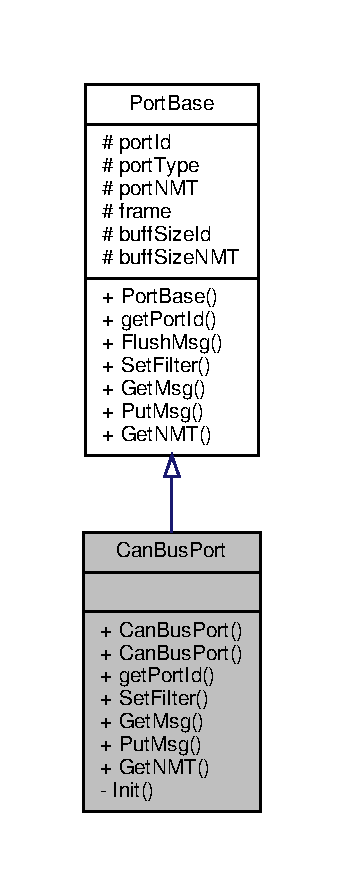
\includegraphics[width=150pt]{classCanBusPort__inherit__graph}
\end{center}
\end{figure}


Collaboration diagram for Can\+Bus\+Port\+:
\nopagebreak
\begin{figure}[H]
\begin{center}
\leavevmode
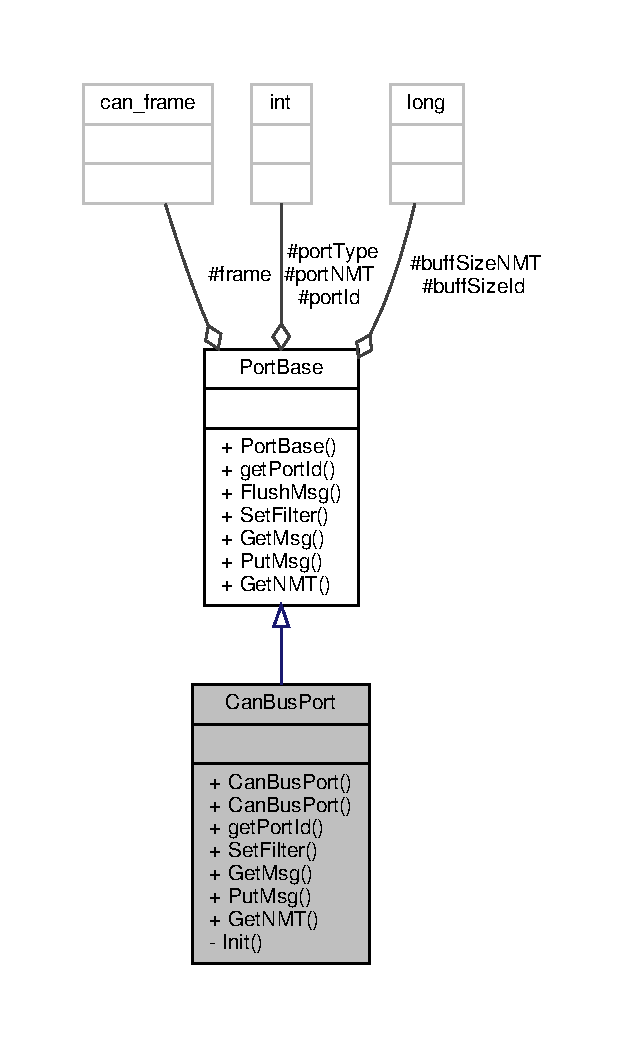
\includegraphics[width=150pt]{classCanBusPort__coll__graph}
\end{center}
\end{figure}
\subsection*{Public Member Functions}
\begin{DoxyCompactItemize}
\item 
\mbox{\Hypertarget{classCanBusPort_a4ccb8d39da6185bfe5c1dee38db51987}\label{classCanBusPort_a4ccb8d39da6185bfe5c1dee38db51987}} 
\hyperlink{classCanBusPort_a4ccb8d39da6185bfe5c1dee38db51987}{Can\+Bus\+Port} ()
\begin{DoxyCompactList}\small\item\em \hyperlink{classCanBusPort}{Can\+Bus\+Port}\+: Empty constructor. Initialize default port \char`\"{}/dev/can0\char`\"{}. \end{DoxyCompactList}\item 
\hyperlink{classCanBusPort_ad4649a2da594bbffc267483646fb1405}{Can\+Bus\+Port} (string can\+Port)
\begin{DoxyCompactList}\small\item\em \hyperlink{classCanBusPort}{Can\+Bus\+Port}\+: Initialization of one port given a device name. \end{DoxyCompactList}\item 
\mbox{\Hypertarget{classCanBusPort_a7c6b733c5834d4ab3e1906d847a2234a}\label{classCanBusPort_a7c6b733c5834d4ab3e1906d847a2234a}} 
int {\bfseries get\+Port\+Id} ()
\item 
\mbox{\Hypertarget{classCanBusPort_af09c794e3af86e89c8a511535f856dc9}\label{classCanBusPort_af09c794e3af86e89c8a511535f856dc9}} 
long {\bfseries Set\+Filter} (uint32\+\_\+t can\+Id, uint32\+\_\+t mask)
\item 
\mbox{\Hypertarget{classCanBusPort_a13d6b06d93debc20b2f49aa8e7139988}\label{classCanBusPort_a13d6b06d93debc20b2f49aa8e7139988}} 
long {\bfseries Get\+Msg} (uint32\+\_\+t \&can\+Id, uint8\+\_\+t $\ast$data, uint8\+\_\+t size)
\item 
\mbox{\Hypertarget{classCanBusPort_a2bb802ad7a14e260f0f51b79d4c53c43}\label{classCanBusPort_a2bb802ad7a14e260f0f51b79d4c53c43}} 
long {\bfseries Put\+Msg} (const uint32\+\_\+t \&can\+Id, uint8\+\_\+t $\ast$const data, const uint8\+\_\+t size)
\item 
\mbox{\Hypertarget{classCanBusPort_a41242dc7980ca398e4770813e50ef32b}\label{classCanBusPort_a41242dc7980ca398e4770813e50ef32b}} 
long {\bfseries Get\+N\+MT} (uint8\+\_\+t $\ast$const data, uint8\+\_\+t \&size)
\end{DoxyCompactItemize}
\subsection*{Additional Inherited Members}


\subsection{Constructor \& Destructor Documentation}
\mbox{\Hypertarget{classCanBusPort_ad4649a2da594bbffc267483646fb1405}\label{classCanBusPort_ad4649a2da594bbffc267483646fb1405}} 
\index{Can\+Bus\+Port@{Can\+Bus\+Port}!Can\+Bus\+Port@{Can\+Bus\+Port}}
\index{Can\+Bus\+Port@{Can\+Bus\+Port}!Can\+Bus\+Port@{Can\+Bus\+Port}}
\subsubsection{\texorpdfstring{Can\+Bus\+Port()}{CanBusPort()}}
{\footnotesize\ttfamily Can\+Bus\+Port\+::\+Can\+Bus\+Port (\begin{DoxyParamCaption}\item[{string}]{can\+Port }\end{DoxyParamCaption})}



\hyperlink{classCanBusPort}{Can\+Bus\+Port}\+: Initialization of one port given a device name. 


\begin{DoxyParams}{Parameters}
{\em can\+Port} & String with the name of system device. \\
\hline
\end{DoxyParams}


The documentation for this class was generated from the following files\+:\begin{DoxyCompactItemize}
\item 
Can\+Bus\+Port.\+h\item 
Can\+Bus\+Port.\+cpp\end{DoxyCompactItemize}

\hypertarget{classCiA301CommPort}{}\section{Ci\+A301\+Comm\+Port Class Reference}
\label{classCiA301CommPort}\index{Ci\+A301\+Comm\+Port@{Ci\+A301\+Comm\+Port}}


{\ttfamily \#include $<$Ci\+A301\+Comm\+Port.\+h$>$}



Inheritance diagram for Ci\+A301\+Comm\+Port\+:\nopagebreak
\begin{figure}[H]
\begin{center}
\leavevmode
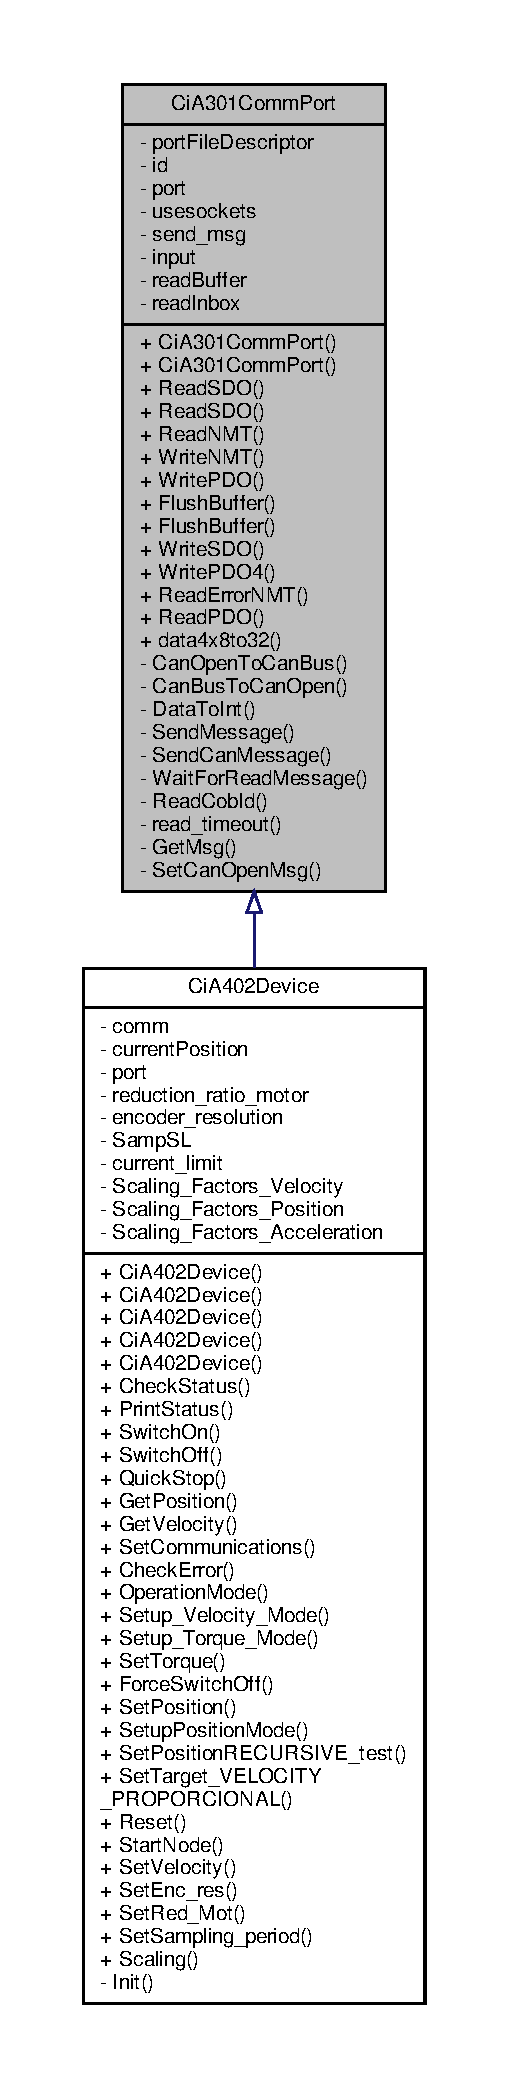
\includegraphics[height=550pt]{classCiA301CommPort__inherit__graph}
\end{center}
\end{figure}


Collaboration diagram for Ci\+A301\+Comm\+Port\+:\nopagebreak
\begin{figure}[H]
\begin{center}
\leavevmode
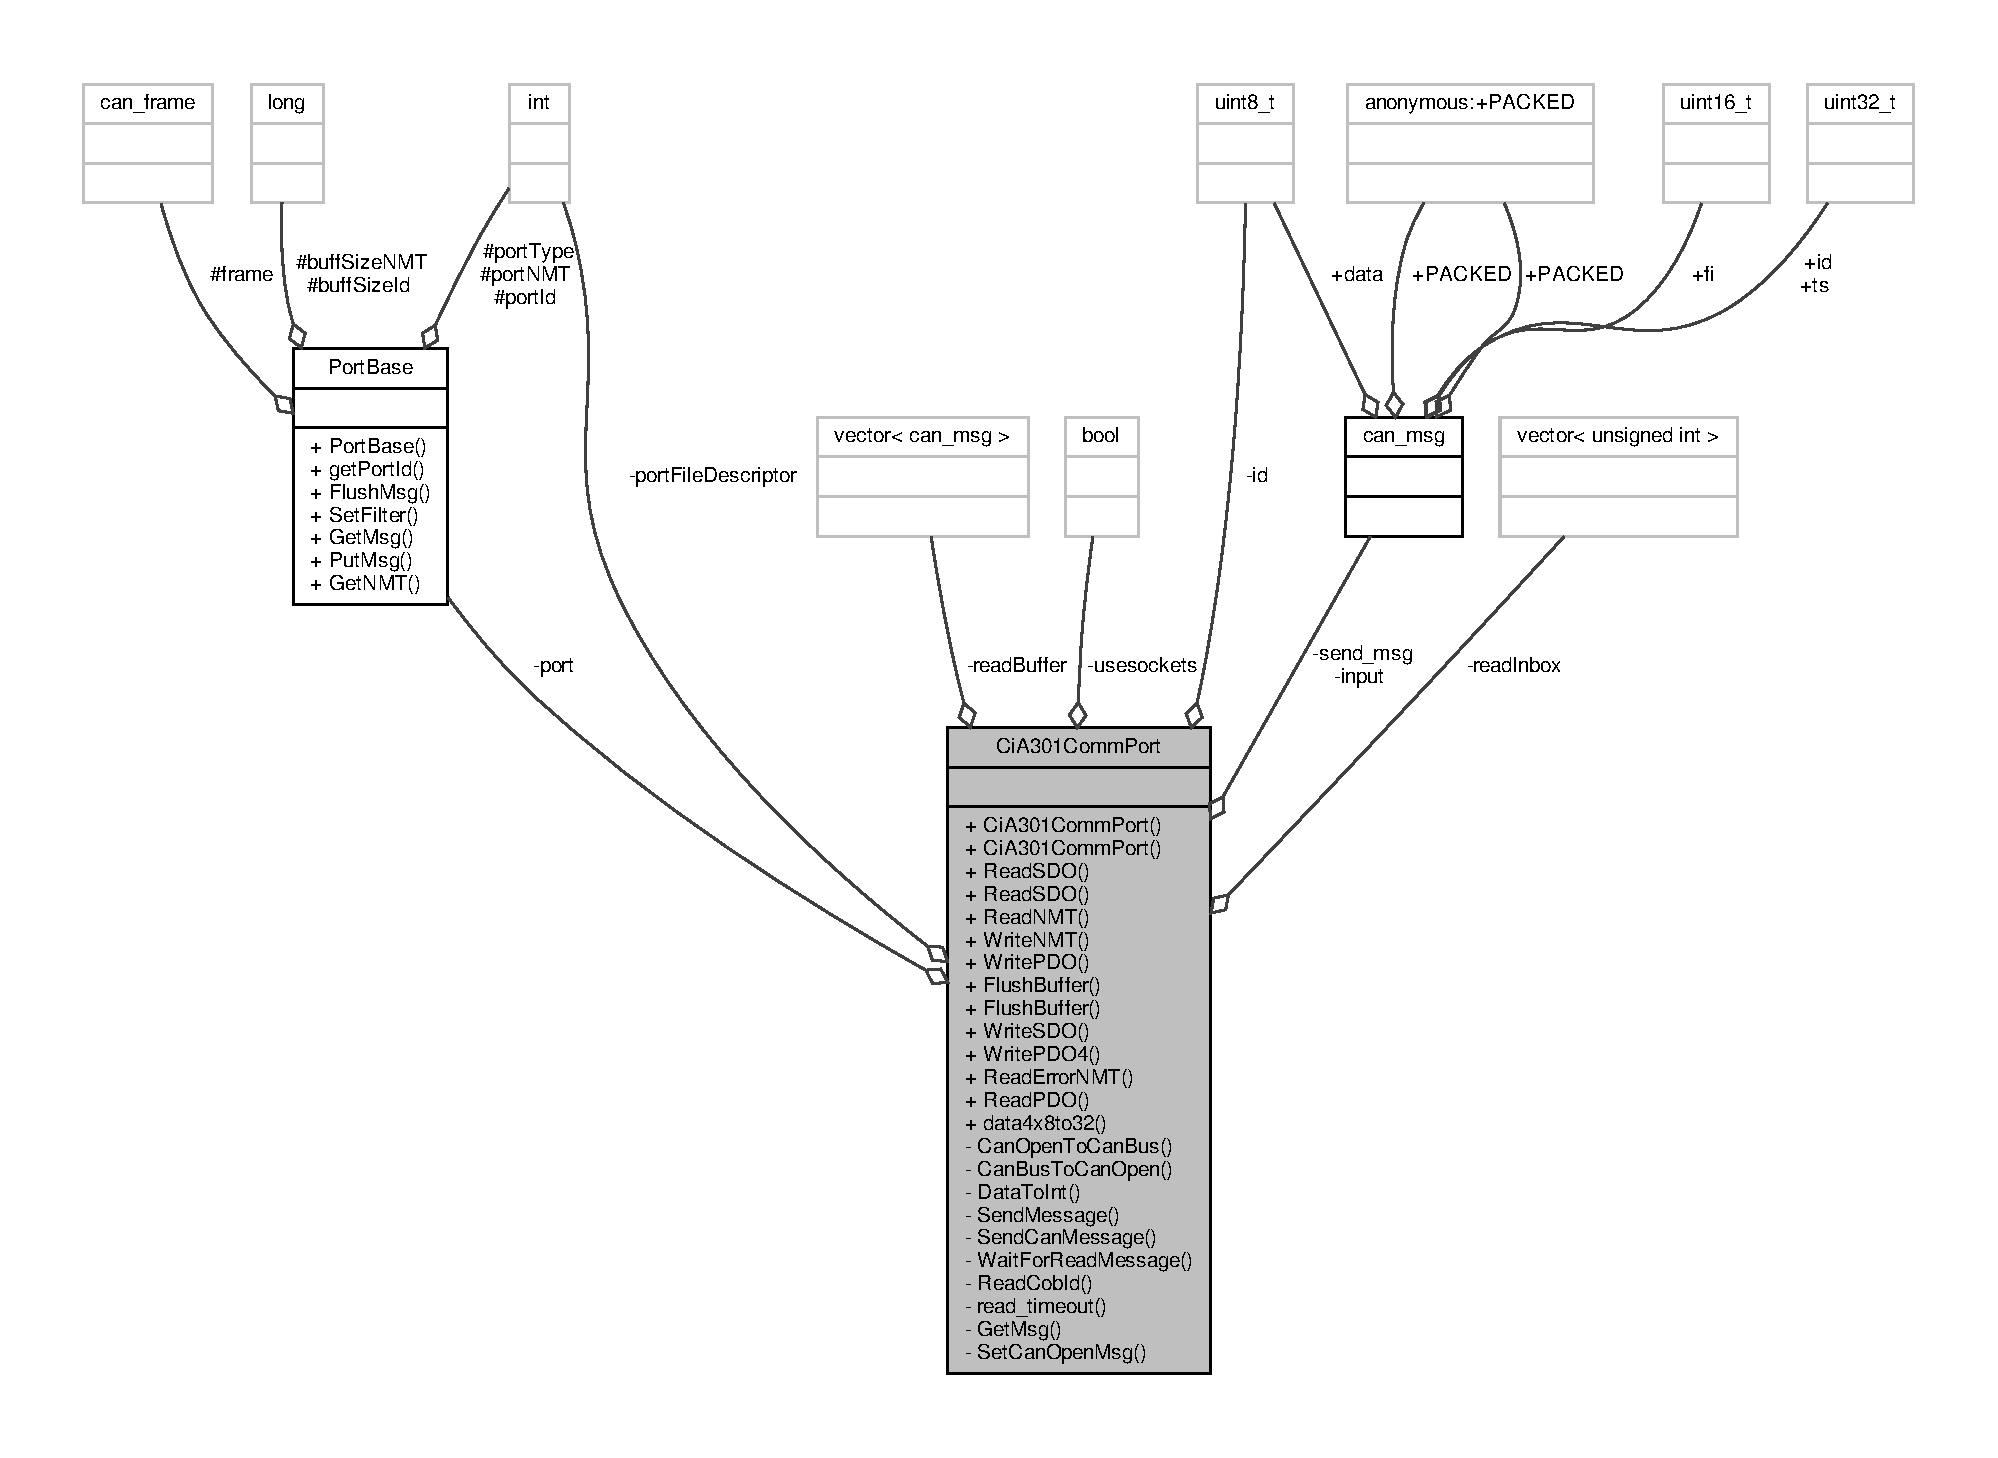
\includegraphics[width=350pt]{classCiA301CommPort__coll__graph}
\end{center}
\end{figure}
\subsection*{Public Member Functions}
\begin{DoxyCompactItemize}
\item 
\hyperlink{classCiA301CommPort_aae705cb5c6a405ef74a10e5220d0b08f}{Ci\+A301\+Comm\+Port} (int new\+Port\+File\+Descriptor, uint8\+\_\+t new\+\_\+id)
\item 
\hyperlink{classCiA301CommPort_a1e05c4b292cfee36ff9eeddb2c8eb4c0}{Ci\+A301\+Comm\+Port} (\hyperlink{classPortBase}{Port\+Base} $\ast$new\+\_\+port, uint8\+\_\+t new\+\_\+id)
\item 
long \hyperlink{classCiA301CommPort_a0fd0920052684589bc37bb898dcdd758}{Read\+S\+DO} (vector$<$ uint8\+\_\+t $>$ address, int subindex)
\item 
long \hyperlink{classCiA301CommPort_a3f74ce5899b30731322dabd352ccdc55}{Read\+S\+DO} (const vector$<$ uint8\+\_\+t $>$ \&address)
\begin{DoxyCompactList}\small\item\em \hyperlink{classCiA301CommPort_a0fd0920052684589bc37bb898dcdd758}{Ci\+A301\+Comm\+Port\+::\+Read\+S\+DO} Waits until expected. \end{DoxyCompactList}\item 
long \hyperlink{classCiA301CommPort_a02df85ed5140d0d7a57fe0d2f6e47ea1}{Read\+N\+MT} (const vector$<$ uint8\+\_\+t $>$ \&nmt\+Code)
\item 
long \hyperlink{classCiA301CommPort_a09feb3f78831c9fbb683a85cc3bc4562}{Write\+N\+MT} (const vector$<$ uint8\+\_\+t $>$ \&nmt\+Command)
\begin{DoxyCompactList}\small\item\em Write\+N\+MT This function sends N\+MT message from node to Can\+Bus. \end{DoxyCompactList}\item 
long \hyperlink{classCiA301CommPort_a56d2c604b11363e6b287f59b68a546bd}{Write\+P\+DO} (const vector$<$ uint8\+\_\+t $>$ \&command)
\begin{DoxyCompactList}\small\item\em Write\+P\+DO This function sends P\+DO message to a node (the mode id is configured on constructor). \end{DoxyCompactList}\item 
long \hyperlink{classCiA301CommPort_a067cddaf01932fa6fa27255c61b08190}{Flush\+Buffer} ()
\item 
long \hyperlink{classCiA301CommPort_ab29e221039a2d21d1446edb09b91864e}{Flush\+Buffer} (int msgs)
\begin{DoxyCompactList}\small\item\em Flush\+Buffer Removes the msgs number of can frames from buffer. \end{DoxyCompactList}\item 
long \hyperlink{classCiA301CommPort_a4d97c27423b2323f8475f6e5c2f91575}{Write\+S\+DO} (const vector$<$ uint8\+\_\+t $>$ \&address, const vector$<$ uint8\+\_\+t $>$ \&value)
\begin{DoxyCompactList}\small\item\em Write\+S\+DO Writes 4 byte value to specific address on device. This function sends S\+DO message requesting write on the object dictionary address. Also block and wait for the S\+DO msg for write ack, and returns negative if error. As it reads the ack S\+DO message, the buffer should be same size after this function returns. \end{DoxyCompactList}\item 
long \hyperlink{classCiA301CommPort_a1faf4f37530e0dd0ae4600cfb0b1d742}{Write\+P\+D\+O4} (const vector$<$ uint8\+\_\+t $>$ \&command)
\item 
long \hyperlink{classCiA301CommPort_a46534ff9e7e2a05a0b4913e4331710e5}{Read\+Error\+N\+MT} ()
\item 
long \hyperlink{classCiA301CommPort_a827f3e594b9f1e57a7b7ccb8a278404a}{Read\+P\+DO} (long number)
\end{DoxyCompactItemize}
\subsection*{Private Member Functions}
\begin{DoxyCompactItemize}
\item 
long \hyperlink{classCiA301CommPort_a26346f83700bc8403a315be01c6508e0}{Can\+Open\+To\+Can\+Bus} (const \hyperlink{structco__msg}{co\+\_\+msg} \&\hyperlink{classCiA301CommPort_ae0f955c7141e2067307cea0b48e111d4}{input}, \hyperlink{structcan__msg}{can\+\_\+msg} \&output)
\item 
long \hyperlink{classCiA301CommPort_aa16887712ea9cad534aacd4851f9190d}{Can\+Bus\+To\+Can\+Open} (const \hyperlink{structcan__msg}{can\+\_\+msg} \&\hyperlink{classCiA301CommPort_ae0f955c7141e2067307cea0b48e111d4}{input}, \hyperlink{structco__msg}{co\+\_\+msg} \&output)
\item 
uint32\+\_\+t \hyperlink{classCiA301CommPort_a77ec43d792a81489e221c3990225e57b}{data4x8to32} (const uint8\+\_\+t $\ast$in)
\item 
uint32\+\_\+t \hyperlink{classCiA301CommPort_a2bbd06fc6ae74727cef148911e433495}{Data\+To\+Int} (const uint8\+\_\+t $\ast$in, const uint8\+\_\+t size)
\item 
int \hyperlink{classCiA301CommPort_aeae04455e1e1a1ca1beed9478372c031}{Send\+Message} (\hyperlink{structco__msg}{co\+\_\+msg} \hyperlink{classCiA301CommPort_ae0f955c7141e2067307cea0b48e111d4}{input})
\item 
int \hyperlink{classCiA301CommPort_a700a04da67928ca50744617ece28cde5}{Send\+Can\+Message} (\hyperlink{structcan__msg}{can\+\_\+msg} \&\hyperlink{classCiA301CommPort_ae0f955c7141e2067307cea0b48e111d4}{input})
\item 
int \hyperlink{classCiA301CommPort_a02ba7069a0497e3497f3dfaec2879b54}{Wait\+For\+Read\+Message} (\hyperlink{structco__msg}{co\+\_\+msg} \&output, unsigned int can\+Index)
\item 
int \hyperlink{classCiA301CommPort_a408f53d13935a1916ca6f21d08ae135e}{Read\+Cob\+Id} (uint16\+\_\+t expected\+\_\+cobid, \hyperlink{structco__msg}{co\+\_\+msg} \&output)
\begin{DoxyCompactList}\small\item\em Ci\+A301\+Comm\+Port\+::\+Wait\+For\+Answer Read the port until expected canopen answer shows up in the port reads. \end{DoxyCompactList}\item 
int \hyperlink{classCiA301CommPort_ae62c2389b38a0e217aff7ca17a3d87b6}{read\+\_\+timeout} (int fd, \hyperlink{structcan__msg}{can\+\_\+msg} $\ast$buf, unsigned int timeout)
\item 
long \hyperlink{classCiA301CommPort_a645450ca09e07ea6da339923ceeec934}{Get\+Msg} (\hyperlink{structcan__msg}{can\+\_\+msg} \&msg)
\item 
\hyperlink{structco__msg}{co\+\_\+msg} \hyperlink{classCiA301CommPort_a2c197480112989df6bdb9ea89a649636}{Set\+Can\+Open\+Msg} (unsigned short id\+\_\+co, unsigned short rtr, vector$<$ uint8\+\_\+t $>$ co\+Data\+Frame)
\begin{DoxyCompactList}\small\item\em \hyperlink{classCiA402DeviceICanbus_aa439b9175f5879282058a3f4c2edb45d}{Ci\+A402\+Device\+I\+Canbus\+::\+Set\+Can\+Open\+Msg} \+: Constructs canopen message from parameters. \end{DoxyCompactList}\end{DoxyCompactItemize}
\subsection*{Private Attributes}
\begin{DoxyCompactItemize}
\item 
int \hyperlink{classCiA301CommPort_adc50c8d333b18fcb1b5c61ca69ea05c6}{port\+File\+Descriptor}
\item 
uint8\+\_\+t \hyperlink{classCiA301CommPort_a1ae075d22fc854da21a6e691bb029fc0}{id}
\item 
\hyperlink{classPortBase}{Port\+Base} $\ast$ \hyperlink{classCiA301CommPort_a6b8366387075c99ee980d2ca79c7b7fc}{port}
\item 
bool \hyperlink{classCiA301CommPort_a579e0de814111bde3bbe18cceb76ce64}{usesockets}
\item 
\hyperlink{structcan__msg}{can\+\_\+msg} \hyperlink{classCiA301CommPort_ade81ac897a5d851d946dd7a18245b75d}{send\+\_\+msg}
\item 
\hyperlink{structcan__msg}{can\+\_\+msg} \hyperlink{classCiA301CommPort_ae0f955c7141e2067307cea0b48e111d4}{input}
\item 
vector$<$ \hyperlink{structcan__msg}{can\+\_\+msg} $>$ \hyperlink{classCiA301CommPort_a8b904f3591ecfb99fd82271343727215}{read\+Buffer}
\item 
vector$<$ unsigned int $>$ \hyperlink{classCiA301CommPort_a41b2fcb24a27e5280417db03d8cdb399}{read\+Inbox}
\end{DoxyCompactItemize}


\subsection{Constructor \& Destructor Documentation}
\mbox{\Hypertarget{classCiA301CommPort_aae705cb5c6a405ef74a10e5220d0b08f}\label{classCiA301CommPort_aae705cb5c6a405ef74a10e5220d0b08f}} 
\index{Ci\+A301\+Comm\+Port@{Ci\+A301\+Comm\+Port}!Ci\+A301\+Comm\+Port@{Ci\+A301\+Comm\+Port}}
\index{Ci\+A301\+Comm\+Port@{Ci\+A301\+Comm\+Port}!Ci\+A301\+Comm\+Port@{Ci\+A301\+Comm\+Port}}
\subsubsection{\texorpdfstring{Ci\+A301\+Comm\+Port()}{CiA301CommPort()}\hspace{0.1cm}{\footnotesize\ttfamily [1/2]}}
{\footnotesize\ttfamily Ci\+A301\+Comm\+Port\+::\+Ci\+A301\+Comm\+Port (\begin{DoxyParamCaption}\item[{int}]{new\+Port\+File\+Descriptor,  }\item[{uint8\+\_\+t}]{new\+\_\+id }\end{DoxyParamCaption})}

\mbox{\Hypertarget{classCiA301CommPort_a1e05c4b292cfee36ff9eeddb2c8eb4c0}\label{classCiA301CommPort_a1e05c4b292cfee36ff9eeddb2c8eb4c0}} 
\index{Ci\+A301\+Comm\+Port@{Ci\+A301\+Comm\+Port}!Ci\+A301\+Comm\+Port@{Ci\+A301\+Comm\+Port}}
\index{Ci\+A301\+Comm\+Port@{Ci\+A301\+Comm\+Port}!Ci\+A301\+Comm\+Port@{Ci\+A301\+Comm\+Port}}
\subsubsection{\texorpdfstring{Ci\+A301\+Comm\+Port()}{CiA301CommPort()}\hspace{0.1cm}{\footnotesize\ttfamily [2/2]}}
{\footnotesize\ttfamily Ci\+A301\+Comm\+Port\+::\+Ci\+A301\+Comm\+Port (\begin{DoxyParamCaption}\item[{\hyperlink{classPortBase}{Port\+Base} $\ast$}]{new\+\_\+port,  }\item[{uint8\+\_\+t}]{new\+\_\+id }\end{DoxyParamCaption})}



\subsection{Member Function Documentation}
\mbox{\Hypertarget{classCiA301CommPort_aa16887712ea9cad534aacd4851f9190d}\label{classCiA301CommPort_aa16887712ea9cad534aacd4851f9190d}} 
\index{Ci\+A301\+Comm\+Port@{Ci\+A301\+Comm\+Port}!Can\+Bus\+To\+Can\+Open@{Can\+Bus\+To\+Can\+Open}}
\index{Can\+Bus\+To\+Can\+Open@{Can\+Bus\+To\+Can\+Open}!Ci\+A301\+Comm\+Port@{Ci\+A301\+Comm\+Port}}
\subsubsection{\texorpdfstring{Can\+Bus\+To\+Can\+Open()}{CanBusToCanOpen()}}
{\footnotesize\ttfamily long Ci\+A301\+Comm\+Port\+::\+Can\+Bus\+To\+Can\+Open (\begin{DoxyParamCaption}\item[{const \hyperlink{structcan__msg}{can\+\_\+msg} \&}]{input,  }\item[{\hyperlink{structco__msg}{co\+\_\+msg} \&}]{output }\end{DoxyParamCaption})\hspace{0.3cm}{\ttfamily [private]}}

\mbox{\Hypertarget{classCiA301CommPort_a26346f83700bc8403a315be01c6508e0}\label{classCiA301CommPort_a26346f83700bc8403a315be01c6508e0}} 
\index{Ci\+A301\+Comm\+Port@{Ci\+A301\+Comm\+Port}!Can\+Open\+To\+Can\+Bus@{Can\+Open\+To\+Can\+Bus}}
\index{Can\+Open\+To\+Can\+Bus@{Can\+Open\+To\+Can\+Bus}!Ci\+A301\+Comm\+Port@{Ci\+A301\+Comm\+Port}}
\subsubsection{\texorpdfstring{Can\+Open\+To\+Can\+Bus()}{CanOpenToCanBus()}}
{\footnotesize\ttfamily long Ci\+A301\+Comm\+Port\+::\+Can\+Open\+To\+Can\+Bus (\begin{DoxyParamCaption}\item[{const \hyperlink{structco__msg}{co\+\_\+msg} \&}]{input,  }\item[{\hyperlink{structcan__msg}{can\+\_\+msg} \&}]{output }\end{DoxyParamCaption})\hspace{0.3cm}{\ttfamily [private]}}

\mbox{\Hypertarget{classCiA301CommPort_a77ec43d792a81489e221c3990225e57b}\label{classCiA301CommPort_a77ec43d792a81489e221c3990225e57b}} 
\index{Ci\+A301\+Comm\+Port@{Ci\+A301\+Comm\+Port}!data4x8to32@{data4x8to32}}
\index{data4x8to32@{data4x8to32}!Ci\+A301\+Comm\+Port@{Ci\+A301\+Comm\+Port}}
\subsubsection{\texorpdfstring{data4x8to32()}{data4x8to32()}}
{\footnotesize\ttfamily uint32\+\_\+t Ci\+A301\+Comm\+Port\+::data4x8to32 (\begin{DoxyParamCaption}\item[{const uint8\+\_\+t $\ast$}]{in }\end{DoxyParamCaption})\hspace{0.3cm}{\ttfamily [private]}}

\mbox{\Hypertarget{classCiA301CommPort_a2bbd06fc6ae74727cef148911e433495}\label{classCiA301CommPort_a2bbd06fc6ae74727cef148911e433495}} 
\index{Ci\+A301\+Comm\+Port@{Ci\+A301\+Comm\+Port}!Data\+To\+Int@{Data\+To\+Int}}
\index{Data\+To\+Int@{Data\+To\+Int}!Ci\+A301\+Comm\+Port@{Ci\+A301\+Comm\+Port}}
\subsubsection{\texorpdfstring{Data\+To\+Int()}{DataToInt()}}
{\footnotesize\ttfamily uint32\+\_\+t Ci\+A301\+Comm\+Port\+::\+Data\+To\+Int (\begin{DoxyParamCaption}\item[{const uint8\+\_\+t $\ast$}]{in,  }\item[{const uint8\+\_\+t}]{size }\end{DoxyParamCaption})\hspace{0.3cm}{\ttfamily [private]}}

\mbox{\Hypertarget{classCiA301CommPort_a067cddaf01932fa6fa27255c61b08190}\label{classCiA301CommPort_a067cddaf01932fa6fa27255c61b08190}} 
\index{Ci\+A301\+Comm\+Port@{Ci\+A301\+Comm\+Port}!Flush\+Buffer@{Flush\+Buffer}}
\index{Flush\+Buffer@{Flush\+Buffer}!Ci\+A301\+Comm\+Port@{Ci\+A301\+Comm\+Port}}
\subsubsection{\texorpdfstring{Flush\+Buffer()}{FlushBuffer()}\hspace{0.1cm}{\footnotesize\ttfamily [1/2]}}
{\footnotesize\ttfamily long Ci\+A301\+Comm\+Port\+::\+Flush\+Buffer (\begin{DoxyParamCaption}{ }\end{DoxyParamCaption})}

\mbox{\Hypertarget{classCiA301CommPort_ab29e221039a2d21d1446edb09b91864e}\label{classCiA301CommPort_ab29e221039a2d21d1446edb09b91864e}} 
\index{Ci\+A301\+Comm\+Port@{Ci\+A301\+Comm\+Port}!Flush\+Buffer@{Flush\+Buffer}}
\index{Flush\+Buffer@{Flush\+Buffer}!Ci\+A301\+Comm\+Port@{Ci\+A301\+Comm\+Port}}
\subsubsection{\texorpdfstring{Flush\+Buffer()}{FlushBuffer()}\hspace{0.1cm}{\footnotesize\ttfamily [2/2]}}
{\footnotesize\ttfamily long Ci\+A301\+Comm\+Port\+::\+Flush\+Buffer (\begin{DoxyParamCaption}\item[{int}]{msgs }\end{DoxyParamCaption})}



Flush\+Buffer Removes the msgs number of can frames from buffer. 


\begin{DoxyParams}{Parameters}
{\em msgs} & Number of messages to remove. \\
\hline
\end{DoxyParams}
\begin{DoxyReturn}{Returns}
0 if no error. 
\end{DoxyReturn}
\mbox{\Hypertarget{classCiA301CommPort_a645450ca09e07ea6da339923ceeec934}\label{classCiA301CommPort_a645450ca09e07ea6da339923ceeec934}} 
\index{Ci\+A301\+Comm\+Port@{Ci\+A301\+Comm\+Port}!Get\+Msg@{Get\+Msg}}
\index{Get\+Msg@{Get\+Msg}!Ci\+A301\+Comm\+Port@{Ci\+A301\+Comm\+Port}}
\subsubsection{\texorpdfstring{Get\+Msg()}{GetMsg()}}
{\footnotesize\ttfamily long Ci\+A301\+Comm\+Port\+::\+Get\+Msg (\begin{DoxyParamCaption}\item[{\hyperlink{structcan__msg}{can\+\_\+msg} \&}]{msg }\end{DoxyParamCaption})\hspace{0.3cm}{\ttfamily [private]}}

\mbox{\Hypertarget{classCiA301CommPort_ae62c2389b38a0e217aff7ca17a3d87b6}\label{classCiA301CommPort_ae62c2389b38a0e217aff7ca17a3d87b6}} 
\index{Ci\+A301\+Comm\+Port@{Ci\+A301\+Comm\+Port}!read\+\_\+timeout@{read\+\_\+timeout}}
\index{read\+\_\+timeout@{read\+\_\+timeout}!Ci\+A301\+Comm\+Port@{Ci\+A301\+Comm\+Port}}
\subsubsection{\texorpdfstring{read\+\_\+timeout()}{read\_timeout()}}
{\footnotesize\ttfamily int Ci\+A301\+Comm\+Port\+::read\+\_\+timeout (\begin{DoxyParamCaption}\item[{int}]{fd,  }\item[{\hyperlink{structcan__msg}{can\+\_\+msg} $\ast$}]{buf,  }\item[{unsigned int}]{timeout }\end{DoxyParamCaption})\hspace{0.3cm}{\ttfamily [private]}}

\mbox{\Hypertarget{classCiA301CommPort_a408f53d13935a1916ca6f21d08ae135e}\label{classCiA301CommPort_a408f53d13935a1916ca6f21d08ae135e}} 
\index{Ci\+A301\+Comm\+Port@{Ci\+A301\+Comm\+Port}!Read\+Cob\+Id@{Read\+Cob\+Id}}
\index{Read\+Cob\+Id@{Read\+Cob\+Id}!Ci\+A301\+Comm\+Port@{Ci\+A301\+Comm\+Port}}
\subsubsection{\texorpdfstring{Read\+Cob\+Id()}{ReadCobId()}}
{\footnotesize\ttfamily int Ci\+A301\+Comm\+Port\+::\+Read\+Cob\+Id (\begin{DoxyParamCaption}\item[{uint16\+\_\+t}]{expected\+\_\+cobid,  }\item[{\hyperlink{structco__msg}{co\+\_\+msg} \&}]{output }\end{DoxyParamCaption})\hspace{0.3cm}{\ttfamily [private]}}



Ci\+A301\+Comm\+Port\+::\+Wait\+For\+Answer Read the port until expected canopen answer shows up in the port reads. 


\begin{DoxyParams}{Parameters}
{\em output} & Expected canopen answer. \\
\hline
{\em can\+Index} & Index of the caller. \\
\hline
\end{DoxyParams}
\begin{DoxyReturn}{Returns}

\end{DoxyReturn}
\mbox{\Hypertarget{classCiA301CommPort_a46534ff9e7e2a05a0b4913e4331710e5}\label{classCiA301CommPort_a46534ff9e7e2a05a0b4913e4331710e5}} 
\index{Ci\+A301\+Comm\+Port@{Ci\+A301\+Comm\+Port}!Read\+Error\+N\+MT@{Read\+Error\+N\+MT}}
\index{Read\+Error\+N\+MT@{Read\+Error\+N\+MT}!Ci\+A301\+Comm\+Port@{Ci\+A301\+Comm\+Port}}
\subsubsection{\texorpdfstring{Read\+Error\+N\+M\+T()}{ReadErrorNMT()}}
{\footnotesize\ttfamily long Ci\+A301\+Comm\+Port\+::\+Read\+Error\+N\+MT (\begin{DoxyParamCaption}{ }\end{DoxyParamCaption})}

\mbox{\Hypertarget{classCiA301CommPort_a02df85ed5140d0d7a57fe0d2f6e47ea1}\label{classCiA301CommPort_a02df85ed5140d0d7a57fe0d2f6e47ea1}} 
\index{Ci\+A301\+Comm\+Port@{Ci\+A301\+Comm\+Port}!Read\+N\+MT@{Read\+N\+MT}}
\index{Read\+N\+MT@{Read\+N\+MT}!Ci\+A301\+Comm\+Port@{Ci\+A301\+Comm\+Port}}
\subsubsection{\texorpdfstring{Read\+N\+M\+T()}{ReadNMT()}}
{\footnotesize\ttfamily long Ci\+A301\+Comm\+Port\+::\+Read\+N\+MT (\begin{DoxyParamCaption}\item[{const vector$<$ uint8\+\_\+t $>$ \&}]{nmt\+Code }\end{DoxyParamCaption})}

\mbox{\Hypertarget{classCiA301CommPort_a827f3e594b9f1e57a7b7ccb8a278404a}\label{classCiA301CommPort_a827f3e594b9f1e57a7b7ccb8a278404a}} 
\index{Ci\+A301\+Comm\+Port@{Ci\+A301\+Comm\+Port}!Read\+P\+DO@{Read\+P\+DO}}
\index{Read\+P\+DO@{Read\+P\+DO}!Ci\+A301\+Comm\+Port@{Ci\+A301\+Comm\+Port}}
\subsubsection{\texorpdfstring{Read\+P\+D\+O()}{ReadPDO()}}
{\footnotesize\ttfamily long Ci\+A301\+Comm\+Port\+::\+Read\+P\+DO (\begin{DoxyParamCaption}\item[{long}]{number }\end{DoxyParamCaption})}

\mbox{\Hypertarget{classCiA301CommPort_a0fd0920052684589bc37bb898dcdd758}\label{classCiA301CommPort_a0fd0920052684589bc37bb898dcdd758}} 
\index{Ci\+A301\+Comm\+Port@{Ci\+A301\+Comm\+Port}!Read\+S\+DO@{Read\+S\+DO}}
\index{Read\+S\+DO@{Read\+S\+DO}!Ci\+A301\+Comm\+Port@{Ci\+A301\+Comm\+Port}}
\subsubsection{\texorpdfstring{Read\+S\+D\+O()}{ReadSDO()}\hspace{0.1cm}{\footnotesize\ttfamily [1/2]}}
{\footnotesize\ttfamily long Ci\+A301\+Comm\+Port\+::\+Read\+S\+DO (\begin{DoxyParamCaption}\item[{vector$<$ uint8\+\_\+t $>$}]{address,  }\item[{int}]{subindex }\end{DoxyParamCaption})}

\mbox{\Hypertarget{classCiA301CommPort_a3f74ce5899b30731322dabd352ccdc55}\label{classCiA301CommPort_a3f74ce5899b30731322dabd352ccdc55}} 
\index{Ci\+A301\+Comm\+Port@{Ci\+A301\+Comm\+Port}!Read\+S\+DO@{Read\+S\+DO}}
\index{Read\+S\+DO@{Read\+S\+DO}!Ci\+A301\+Comm\+Port@{Ci\+A301\+Comm\+Port}}
\subsubsection{\texorpdfstring{Read\+S\+D\+O()}{ReadSDO()}\hspace{0.1cm}{\footnotesize\ttfamily [2/2]}}
{\footnotesize\ttfamily long Ci\+A301\+Comm\+Port\+::\+Read\+S\+DO (\begin{DoxyParamCaption}\item[{const vector$<$ uint8\+\_\+t $>$ \&}]{address }\end{DoxyParamCaption})}



\hyperlink{classCiA301CommPort_a0fd0920052684589bc37bb898dcdd758}{Ci\+A301\+Comm\+Port\+::\+Read\+S\+DO} Waits until expected. 


\begin{DoxyParams}{Parameters}
{\em address} & \\
\hline
\end{DoxyParams}
\begin{DoxyReturn}{Returns}

\end{DoxyReturn}
\mbox{\Hypertarget{classCiA301CommPort_a700a04da67928ca50744617ece28cde5}\label{classCiA301CommPort_a700a04da67928ca50744617ece28cde5}} 
\index{Ci\+A301\+Comm\+Port@{Ci\+A301\+Comm\+Port}!Send\+Can\+Message@{Send\+Can\+Message}}
\index{Send\+Can\+Message@{Send\+Can\+Message}!Ci\+A301\+Comm\+Port@{Ci\+A301\+Comm\+Port}}
\subsubsection{\texorpdfstring{Send\+Can\+Message()}{SendCanMessage()}}
{\footnotesize\ttfamily int Ci\+A301\+Comm\+Port\+::\+Send\+Can\+Message (\begin{DoxyParamCaption}\item[{\hyperlink{structcan__msg}{can\+\_\+msg} \&}]{input }\end{DoxyParamCaption})\hspace{0.3cm}{\ttfamily [private]}}

\mbox{\Hypertarget{classCiA301CommPort_aeae04455e1e1a1ca1beed9478372c031}\label{classCiA301CommPort_aeae04455e1e1a1ca1beed9478372c031}} 
\index{Ci\+A301\+Comm\+Port@{Ci\+A301\+Comm\+Port}!Send\+Message@{Send\+Message}}
\index{Send\+Message@{Send\+Message}!Ci\+A301\+Comm\+Port@{Ci\+A301\+Comm\+Port}}
\subsubsection{\texorpdfstring{Send\+Message()}{SendMessage()}}
{\footnotesize\ttfamily int Ci\+A301\+Comm\+Port\+::\+Send\+Message (\begin{DoxyParamCaption}\item[{\hyperlink{structco__msg}{co\+\_\+msg}}]{input }\end{DoxyParamCaption})\hspace{0.3cm}{\ttfamily [private]}}

\mbox{\Hypertarget{classCiA301CommPort_a2c197480112989df6bdb9ea89a649636}\label{classCiA301CommPort_a2c197480112989df6bdb9ea89a649636}} 
\index{Ci\+A301\+Comm\+Port@{Ci\+A301\+Comm\+Port}!Set\+Can\+Open\+Msg@{Set\+Can\+Open\+Msg}}
\index{Set\+Can\+Open\+Msg@{Set\+Can\+Open\+Msg}!Ci\+A301\+Comm\+Port@{Ci\+A301\+Comm\+Port}}
\subsubsection{\texorpdfstring{Set\+Can\+Open\+Msg()}{SetCanOpenMsg()}}
{\footnotesize\ttfamily \hyperlink{structco__msg}{co\+\_\+msg} Ci\+A301\+Comm\+Port\+::\+Set\+Can\+Open\+Msg (\begin{DoxyParamCaption}\item[{unsigned short}]{id\+\_\+co,  }\item[{unsigned short}]{rtr,  }\item[{vector$<$ uint8\+\_\+t $>$}]{co\+Data\+Frame }\end{DoxyParamCaption})\hspace{0.3cm}{\ttfamily [private]}}



\hyperlink{classCiA402DeviceICanbus_aa439b9175f5879282058a3f4c2edb45d}{Ci\+A402\+Device\+I\+Canbus\+::\+Set\+Can\+Open\+Msg} \+: Constructs canopen message from parameters. 


\begin{DoxyParams}{Parameters}
{\em id\+\_\+co} & cob id canopen parameter. \\
\hline
{\em rtr} & request for remote. \\
\hline
{\em msg\+\_\+start} & \+: canopen data frame. \\
\hline
\end{DoxyParams}
\begin{DoxyReturn}{Returns}
\+: canopen constructed message in \hyperlink{structco__msg}{co\+\_\+msg} data type. 
\end{DoxyReturn}
\mbox{\Hypertarget{classCiA301CommPort_a02ba7069a0497e3497f3dfaec2879b54}\label{classCiA301CommPort_a02ba7069a0497e3497f3dfaec2879b54}} 
\index{Ci\+A301\+Comm\+Port@{Ci\+A301\+Comm\+Port}!Wait\+For\+Read\+Message@{Wait\+For\+Read\+Message}}
\index{Wait\+For\+Read\+Message@{Wait\+For\+Read\+Message}!Ci\+A301\+Comm\+Port@{Ci\+A301\+Comm\+Port}}
\subsubsection{\texorpdfstring{Wait\+For\+Read\+Message()}{WaitForReadMessage()}}
{\footnotesize\ttfamily int Ci\+A301\+Comm\+Port\+::\+Wait\+For\+Read\+Message (\begin{DoxyParamCaption}\item[{\hyperlink{structco__msg}{co\+\_\+msg} \&}]{output,  }\item[{unsigned int}]{can\+Index }\end{DoxyParamCaption})\hspace{0.3cm}{\ttfamily [private]}}

\mbox{\Hypertarget{classCiA301CommPort_a09feb3f78831c9fbb683a85cc3bc4562}\label{classCiA301CommPort_a09feb3f78831c9fbb683a85cc3bc4562}} 
\index{Ci\+A301\+Comm\+Port@{Ci\+A301\+Comm\+Port}!Write\+N\+MT@{Write\+N\+MT}}
\index{Write\+N\+MT@{Write\+N\+MT}!Ci\+A301\+Comm\+Port@{Ci\+A301\+Comm\+Port}}
\subsubsection{\texorpdfstring{Write\+N\+M\+T()}{WriteNMT()}}
{\footnotesize\ttfamily long Ci\+A301\+Comm\+Port\+::\+Write\+N\+MT (\begin{DoxyParamCaption}\item[{const vector$<$ uint8\+\_\+t $>$ \&}]{nmt\+Command }\end{DoxyParamCaption})}



Write\+N\+MT This function sends N\+MT message from node to Can\+Bus. 


\begin{DoxyParams}{Parameters}
{\em nmt\+Command} & The message that is sent. \\
\hline
\end{DoxyParams}
\begin{DoxyReturn}{Returns}
0 if no error. 
\end{DoxyReturn}
\mbox{\Hypertarget{classCiA301CommPort_a56d2c604b11363e6b287f59b68a546bd}\label{classCiA301CommPort_a56d2c604b11363e6b287f59b68a546bd}} 
\index{Ci\+A301\+Comm\+Port@{Ci\+A301\+Comm\+Port}!Write\+P\+DO@{Write\+P\+DO}}
\index{Write\+P\+DO@{Write\+P\+DO}!Ci\+A301\+Comm\+Port@{Ci\+A301\+Comm\+Port}}
\subsubsection{\texorpdfstring{Write\+P\+D\+O()}{WritePDO()}}
{\footnotesize\ttfamily long Ci\+A301\+Comm\+Port\+::\+Write\+P\+DO (\begin{DoxyParamCaption}\item[{const vector$<$ uint8\+\_\+t $>$ \&}]{command }\end{DoxyParamCaption})}



Write\+P\+DO This function sends P\+DO message to a node (the mode id is configured on constructor). 


\begin{DoxyParams}{Parameters}
{\em command} & The mesage that is sent. \\
\hline
\end{DoxyParams}
\begin{DoxyReturn}{Returns}
0 if no error. 
\end{DoxyReturn}
\mbox{\Hypertarget{classCiA301CommPort_a1faf4f37530e0dd0ae4600cfb0b1d742}\label{classCiA301CommPort_a1faf4f37530e0dd0ae4600cfb0b1d742}} 
\index{Ci\+A301\+Comm\+Port@{Ci\+A301\+Comm\+Port}!Write\+P\+D\+O4@{Write\+P\+D\+O4}}
\index{Write\+P\+D\+O4@{Write\+P\+D\+O4}!Ci\+A301\+Comm\+Port@{Ci\+A301\+Comm\+Port}}
\subsubsection{\texorpdfstring{Write\+P\+D\+O4()}{WritePDO4()}}
{\footnotesize\ttfamily long Ci\+A301\+Comm\+Port\+::\+Write\+P\+D\+O4 (\begin{DoxyParamCaption}\item[{const vector$<$ uint8\+\_\+t $>$ \&}]{command }\end{DoxyParamCaption})}

\mbox{\Hypertarget{classCiA301CommPort_a4d97c27423b2323f8475f6e5c2f91575}\label{classCiA301CommPort_a4d97c27423b2323f8475f6e5c2f91575}} 
\index{Ci\+A301\+Comm\+Port@{Ci\+A301\+Comm\+Port}!Write\+S\+DO@{Write\+S\+DO}}
\index{Write\+S\+DO@{Write\+S\+DO}!Ci\+A301\+Comm\+Port@{Ci\+A301\+Comm\+Port}}
\subsubsection{\texorpdfstring{Write\+S\+D\+O()}{WriteSDO()}}
{\footnotesize\ttfamily long Ci\+A301\+Comm\+Port\+::\+Write\+S\+DO (\begin{DoxyParamCaption}\item[{const vector$<$ uint8\+\_\+t $>$ \&}]{address,  }\item[{const vector$<$ uint8\+\_\+t $>$ \&}]{value }\end{DoxyParamCaption})}



Write\+S\+DO Writes 4 byte value to specific address on device. This function sends S\+DO message requesting write on the object dictionary address. Also block and wait for the S\+DO msg for write ack, and returns negative if error. As it reads the ack S\+DO message, the buffer should be same size after this function returns. 


\begin{DoxyParams}{Parameters}
{\em address} & The address that needs S\+DO writing. \\
\hline
{\em value} & The value that will be writed. \\
\hline
\end{DoxyParams}
\begin{DoxyReturn}{Returns}
0 if no error. Negative if error (see cerr). 
\end{DoxyReturn}


\subsection{Member Data Documentation}
\mbox{\Hypertarget{classCiA301CommPort_a1ae075d22fc854da21a6e691bb029fc0}\label{classCiA301CommPort_a1ae075d22fc854da21a6e691bb029fc0}} 
\index{Ci\+A301\+Comm\+Port@{Ci\+A301\+Comm\+Port}!id@{id}}
\index{id@{id}!Ci\+A301\+Comm\+Port@{Ci\+A301\+Comm\+Port}}
\subsubsection{\texorpdfstring{id}{id}}
{\footnotesize\ttfamily uint8\+\_\+t Ci\+A301\+Comm\+Port\+::id\hspace{0.3cm}{\ttfamily [private]}}

\mbox{\Hypertarget{classCiA301CommPort_ae0f955c7141e2067307cea0b48e111d4}\label{classCiA301CommPort_ae0f955c7141e2067307cea0b48e111d4}} 
\index{Ci\+A301\+Comm\+Port@{Ci\+A301\+Comm\+Port}!input@{input}}
\index{input@{input}!Ci\+A301\+Comm\+Port@{Ci\+A301\+Comm\+Port}}
\subsubsection{\texorpdfstring{input}{input}}
{\footnotesize\ttfamily \hyperlink{structcan__msg}{can\+\_\+msg} Ci\+A301\+Comm\+Port\+::input\hspace{0.3cm}{\ttfamily [private]}}

\mbox{\Hypertarget{classCiA301CommPort_a6b8366387075c99ee980d2ca79c7b7fc}\label{classCiA301CommPort_a6b8366387075c99ee980d2ca79c7b7fc}} 
\index{Ci\+A301\+Comm\+Port@{Ci\+A301\+Comm\+Port}!port@{port}}
\index{port@{port}!Ci\+A301\+Comm\+Port@{Ci\+A301\+Comm\+Port}}
\subsubsection{\texorpdfstring{port}{port}}
{\footnotesize\ttfamily \hyperlink{classPortBase}{Port\+Base}$\ast$ Ci\+A301\+Comm\+Port\+::port\hspace{0.3cm}{\ttfamily [private]}}

\mbox{\Hypertarget{classCiA301CommPort_adc50c8d333b18fcb1b5c61ca69ea05c6}\label{classCiA301CommPort_adc50c8d333b18fcb1b5c61ca69ea05c6}} 
\index{Ci\+A301\+Comm\+Port@{Ci\+A301\+Comm\+Port}!port\+File\+Descriptor@{port\+File\+Descriptor}}
\index{port\+File\+Descriptor@{port\+File\+Descriptor}!Ci\+A301\+Comm\+Port@{Ci\+A301\+Comm\+Port}}
\subsubsection{\texorpdfstring{port\+File\+Descriptor}{portFileDescriptor}}
{\footnotesize\ttfamily int Ci\+A301\+Comm\+Port\+::port\+File\+Descriptor\hspace{0.3cm}{\ttfamily [private]}}

\mbox{\Hypertarget{classCiA301CommPort_a8b904f3591ecfb99fd82271343727215}\label{classCiA301CommPort_a8b904f3591ecfb99fd82271343727215}} 
\index{Ci\+A301\+Comm\+Port@{Ci\+A301\+Comm\+Port}!read\+Buffer@{read\+Buffer}}
\index{read\+Buffer@{read\+Buffer}!Ci\+A301\+Comm\+Port@{Ci\+A301\+Comm\+Port}}
\subsubsection{\texorpdfstring{read\+Buffer}{readBuffer}}
{\footnotesize\ttfamily vector$<$\hyperlink{structcan__msg}{can\+\_\+msg}$>$ Ci\+A301\+Comm\+Port\+::read\+Buffer\hspace{0.3cm}{\ttfamily [private]}}

\mbox{\Hypertarget{classCiA301CommPort_a41b2fcb24a27e5280417db03d8cdb399}\label{classCiA301CommPort_a41b2fcb24a27e5280417db03d8cdb399}} 
\index{Ci\+A301\+Comm\+Port@{Ci\+A301\+Comm\+Port}!read\+Inbox@{read\+Inbox}}
\index{read\+Inbox@{read\+Inbox}!Ci\+A301\+Comm\+Port@{Ci\+A301\+Comm\+Port}}
\subsubsection{\texorpdfstring{read\+Inbox}{readInbox}}
{\footnotesize\ttfamily vector$<$unsigned int$>$ Ci\+A301\+Comm\+Port\+::read\+Inbox\hspace{0.3cm}{\ttfamily [private]}}

\mbox{\Hypertarget{classCiA301CommPort_ade81ac897a5d851d946dd7a18245b75d}\label{classCiA301CommPort_ade81ac897a5d851d946dd7a18245b75d}} 
\index{Ci\+A301\+Comm\+Port@{Ci\+A301\+Comm\+Port}!send\+\_\+msg@{send\+\_\+msg}}
\index{send\+\_\+msg@{send\+\_\+msg}!Ci\+A301\+Comm\+Port@{Ci\+A301\+Comm\+Port}}
\subsubsection{\texorpdfstring{send\+\_\+msg}{send\_msg}}
{\footnotesize\ttfamily \hyperlink{structcan__msg}{can\+\_\+msg} Ci\+A301\+Comm\+Port\+::send\+\_\+msg\hspace{0.3cm}{\ttfamily [private]}}

\mbox{\Hypertarget{classCiA301CommPort_a579e0de814111bde3bbe18cceb76ce64}\label{classCiA301CommPort_a579e0de814111bde3bbe18cceb76ce64}} 
\index{Ci\+A301\+Comm\+Port@{Ci\+A301\+Comm\+Port}!usesockets@{usesockets}}
\index{usesockets@{usesockets}!Ci\+A301\+Comm\+Port@{Ci\+A301\+Comm\+Port}}
\subsubsection{\texorpdfstring{usesockets}{usesockets}}
{\footnotesize\ttfamily bool Ci\+A301\+Comm\+Port\+::usesockets\hspace{0.3cm}{\ttfamily [private]}}



The documentation for this class was generated from the following files\+:\begin{DoxyCompactItemize}
\item 
\hyperlink{CiA301CommPort_8h}{Ci\+A301\+Comm\+Port.\+h}\item 
\hyperlink{CiA301CommPort_8cpp}{Ci\+A301\+Comm\+Port.\+cpp}\end{DoxyCompactItemize}

\hypertarget{classCiA402Device}{}\section{Ci\+A402\+Device Class Reference}
\label{classCiA402Device}\index{Ci\+A402\+Device@{Ci\+A402\+Device}}
\subsection*{Public Member Functions}
\begin{DoxyCompactItemize}
\item 
\mbox{\Hypertarget{classCiA402Device_ae71940d1e35a2968a5280bb0f1e5bb5a}\label{classCiA402Device_ae71940d1e35a2968a5280bb0f1e5bb5a}} 
int {\bfseries Check\+Status} ()
\item 
long \hyperlink{classCiA402Device_ab77bce0d7f42429f5f8f092aacb02754}{Switch\+On} ()
\begin{DoxyCompactList}\small\item\em Switch\+On\+: Turn on the device and wait for commands. \end{DoxyCompactList}\item 
long \hyperlink{classCiA402Device_a97acf47b3e3751c85fa70091d3bdfa6a}{Switch\+Off} ()
\begin{DoxyCompactList}\small\item\em Switch\+Off\+: Turn on the device. \end{DoxyCompactList}\item 
double \hyperlink{classCiA402Device_ac8d9e36e6f457565cac7d26d91e4a712}{Get\+Position} ()
\begin{DoxyCompactList}\small\item\em Get\+Position\+: Get the position of the cia 402 device. \end{DoxyCompactList}\end{DoxyCompactItemize}


\subsection{Member Function Documentation}
\mbox{\Hypertarget{classCiA402Device_ac8d9e36e6f457565cac7d26d91e4a712}\label{classCiA402Device_ac8d9e36e6f457565cac7d26d91e4a712}} 
\index{Ci\+A402\+Device@{Ci\+A402\+Device}!Get\+Position@{Get\+Position}}
\index{Get\+Position@{Get\+Position}!Ci\+A402\+Device@{Ci\+A402\+Device}}
\subsubsection{\texorpdfstring{Get\+Position()}{GetPosition()}}
{\footnotesize\ttfamily double Ci\+A402\+Device\+::\+Get\+Position (\begin{DoxyParamCaption}{ }\end{DoxyParamCaption})}



Get\+Position\+: Get the position of the cia 402 device. 

\begin{DoxyReturn}{Returns}
\+: Position (angle in \mbox{[}rad\mbox{]}) 
\end{DoxyReturn}
\mbox{\Hypertarget{classCiA402Device_a97acf47b3e3751c85fa70091d3bdfa6a}\label{classCiA402Device_a97acf47b3e3751c85fa70091d3bdfa6a}} 
\index{Ci\+A402\+Device@{Ci\+A402\+Device}!Switch\+Off@{Switch\+Off}}
\index{Switch\+Off@{Switch\+Off}!Ci\+A402\+Device@{Ci\+A402\+Device}}
\subsubsection{\texorpdfstring{Switch\+Off()}{SwitchOff()}}
{\footnotesize\ttfamily long Ci\+A402\+Device\+::\+Switch\+Off (\begin{DoxyParamCaption}{ }\end{DoxyParamCaption})}



Switch\+Off\+: Turn on the device. 

\begin{DoxyReturn}{Returns}
\+: 0 if correct, negative on errors. 
\end{DoxyReturn}
\mbox{\Hypertarget{classCiA402Device_ab77bce0d7f42429f5f8f092aacb02754}\label{classCiA402Device_ab77bce0d7f42429f5f8f092aacb02754}} 
\index{Ci\+A402\+Device@{Ci\+A402\+Device}!Switch\+On@{Switch\+On}}
\index{Switch\+On@{Switch\+On}!Ci\+A402\+Device@{Ci\+A402\+Device}}
\subsubsection{\texorpdfstring{Switch\+On()}{SwitchOn()}}
{\footnotesize\ttfamily long Ci\+A402\+Device\+::\+Switch\+On (\begin{DoxyParamCaption}{ }\end{DoxyParamCaption})}



Switch\+On\+: Turn on the device and wait for commands. 

\begin{DoxyReturn}{Returns}
\+: 0 if correct, negative on errors. 
\end{DoxyReturn}


The documentation for this class was generated from the following files\+:\begin{DoxyCompactItemize}
\item 
Cia402device.\+h\item 
Cia402device.\+cpp\end{DoxyCompactItemize}

\hypertarget{classCiA402DeviceICanbus}{}\section{Ci\+A402\+Device\+I\+Canbus Class Reference}
\label{classCiA402DeviceICanbus}\index{Ci\+A402\+Device\+I\+Canbus@{Ci\+A402\+Device\+I\+Canbus}}
\subsection*{Public Member Functions}
\begin{DoxyCompactItemize}
\item 
\mbox{\Hypertarget{classCiA402DeviceICanbus_a205b5105bd658b73b582cf1685f1d320}\label{classCiA402DeviceICanbus_a205b5105bd658b73b582cf1685f1d320}} 
{\bfseries Ci\+A402\+Device\+I\+Canbus} (long number, string can\+Port)
\item 
\mbox{\Hypertarget{classCiA402DeviceICanbus_a757447054eadb6824cf779ca58d276ae}\label{classCiA402DeviceICanbus_a757447054eadb6824cf779ca58d276ae}} 
long {\bfseries Init} (const vector$<$ int $>$ \&new\+\_\+can\+Ports, string can\+Port)
\item 
\mbox{\Hypertarget{classCiA402DeviceICanbus_ac831e319febc65d424955e32ecdf72c3}\label{classCiA402DeviceICanbus_ac831e319febc65d424955e32ecdf72c3}} 
int {\bfseries Send\+Message} (\hyperlink{structco__msg}{co\+\_\+msg} input, unsigned int can\+Index)
\item 
\mbox{\Hypertarget{classCiA402DeviceICanbus_aa108188c7f32a1c5d1f50662e66c6676}\label{classCiA402DeviceICanbus_aa108188c7f32a1c5d1f50662e66c6676}} 
long {\bfseries co2c} (const \hyperlink{structco__msg}{co\+\_\+msg} \&input, \hyperlink{structcan__msg}{can\+\_\+msg} \&output)
\item 
\mbox{\Hypertarget{classCiA402DeviceICanbus_a1f8d07b892461470a29ac5d30f3dd679}\label{classCiA402DeviceICanbus_a1f8d07b892461470a29ac5d30f3dd679}} 
int {\bfseries Wait\+For\+Read\+Message} (\hyperlink{structco__msg}{co\+\_\+msg} \&output, unsigned int can\+Index)
\item 
\mbox{\Hypertarget{classCiA402DeviceICanbus_aab504488399b2d5a5a010efef29e3d64}\label{classCiA402DeviceICanbus_aab504488399b2d5a5a010efef29e3d64}} 
long {\bfseries c2co} (const \hyperlink{structcan__msg}{can\+\_\+msg} \&input, \hyperlink{structco__msg}{co\+\_\+msg} \&output)
\item 
\mbox{\Hypertarget{classCiA402DeviceICanbus_aa439b9175f5879282058a3f4c2edb45d}\label{classCiA402DeviceICanbus_aa439b9175f5879282058a3f4c2edb45d}} 
int {\bfseries Set\+Can\+Open\+Msg} (\hyperlink{structco__msg}{co\+\_\+msg} \&msg\+\_\+co)
\item 
\mbox{\Hypertarget{classCiA402DeviceICanbus_af09467b107e73f67804942db1597d983}\label{classCiA402DeviceICanbus_af09467b107e73f67804942db1597d983}} 
int {\bfseries Set\+Can\+Open\+Msg} (\hyperlink{structco__msg}{co\+\_\+msg} \&msg\+\_\+co, uint8\+\_\+t msg\+\_\+start\mbox{[}$\,$\mbox{]})
\item 
\mbox{\Hypertarget{classCiA402DeviceICanbus_a93cde3041c3d0a26666b451aa70b246f}\label{classCiA402DeviceICanbus_a93cde3041c3d0a26666b451aa70b246f}} 
\hyperlink{structcan__msg}{can\+\_\+msg} {\bfseries Set\+Can\+Msg} (\hyperlink{structcan__msg}{can\+\_\+msg} \&msg, uint8\+\_\+t msg\+\_\+start\mbox{[}$\,$\mbox{]})
\item 
\hyperlink{structco__msg}{co\+\_\+msg} \hyperlink{classCiA402DeviceICanbus_ab861fc4d62c917bdb1c06b886c8ed45a}{Set\+Can\+Open\+Msg} (unsigned short id\+\_\+co, unsigned short rtr, vector$<$ uint8\+\_\+t $>$ co\+Data\+Frame)
\begin{DoxyCompactList}\small\item\em Ci\+A402\+Device\+I\+Canbus\+::\+Set\+Can\+Open\+Msg \+: Constructs canopen message from parameters. \end{DoxyCompactList}\end{DoxyCompactItemize}
\subsection*{Public Attributes}
\begin{DoxyCompactItemize}
\item 
\mbox{\Hypertarget{classCiA402DeviceICanbus_a456534a394e4072025f2528938d1070d}\label{classCiA402DeviceICanbus_a456534a394e4072025f2528938d1070d}} 
vector$<$ int $>$ {\bfseries can\+Ports}
\item 
\mbox{\Hypertarget{classCiA402DeviceICanbus_af6cf1493b669ce0415cefed7d84e5710}\label{classCiA402DeviceICanbus_af6cf1493b669ce0415cefed7d84e5710}} 
int {\bfseries ret}
\end{DoxyCompactItemize}


\subsection{Member Function Documentation}
\mbox{\Hypertarget{classCiA402DeviceICanbus_ab861fc4d62c917bdb1c06b886c8ed45a}\label{classCiA402DeviceICanbus_ab861fc4d62c917bdb1c06b886c8ed45a}} 
\index{Ci\+A402\+Device\+I\+Canbus@{Ci\+A402\+Device\+I\+Canbus}!Set\+Can\+Open\+Msg@{Set\+Can\+Open\+Msg}}
\index{Set\+Can\+Open\+Msg@{Set\+Can\+Open\+Msg}!Ci\+A402\+Device\+I\+Canbus@{Ci\+A402\+Device\+I\+Canbus}}
\subsubsection{\texorpdfstring{Set\+Can\+Open\+Msg()}{SetCanOpenMsg()}}
{\footnotesize\ttfamily \hyperlink{structco__msg}{co\+\_\+msg} Ci\+A402\+Device\+I\+Canbus\+::\+Set\+Can\+Open\+Msg (\begin{DoxyParamCaption}\item[{unsigned short}]{id\+\_\+co,  }\item[{unsigned short}]{rtr,  }\item[{vector$<$ uint8\+\_\+t $>$}]{co\+Data\+Frame }\end{DoxyParamCaption})}



Ci\+A402\+Device\+I\+Canbus\+::\+Set\+Can\+Open\+Msg \+: Constructs canopen message from parameters. 


\begin{DoxyParams}{Parameters}
{\em id\+\_\+co} & cob id canopen parameter. \\
\hline
{\em rtr} & request for remote. \\
\hline
{\em msg\+\_\+start} & \+: canopen data frame. \\
\hline
\end{DoxyParams}
\begin{DoxyReturn}{Returns}
\+: canopen constructed message in \hyperlink{structco__msg}{co\+\_\+msg} data type. 
\end{DoxyReturn}


The documentation for this class was generated from the following files\+:\begin{DoxyCompactItemize}
\item 
Ci\+A402\+Device\+I\+Canbus.\+h\item 
Ci\+A402\+Device\+I\+Canbus.\+cpp\end{DoxyCompactItemize}

\hypertarget{classCiA402SetupData}{}\section{Ci\+A402\+Setup\+Data Class Reference}
\label{classCiA402SetupData}\index{Ci\+A402\+Setup\+Data@{Ci\+A402\+Setup\+Data}}


{\ttfamily \#include $<$Ci\+A402\+Setup\+Data.\+h$>$}



Collaboration diagram for Ci\+A402\+Setup\+Data\+:
\nopagebreak
\begin{figure}[H]
\begin{center}
\leavevmode
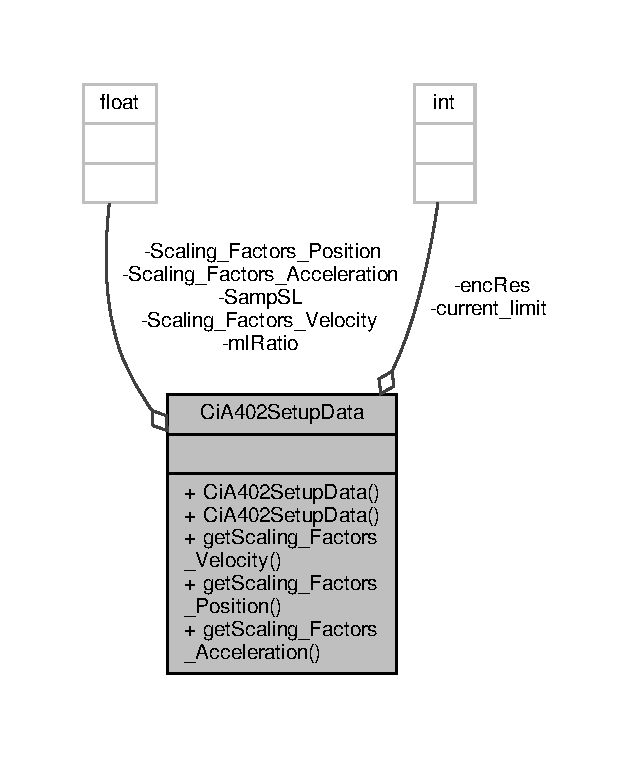
\includegraphics[width=304pt]{classCiA402SetupData__coll__graph}
\end{center}
\end{figure}
\subsection*{Public Member Functions}
\begin{DoxyCompactItemize}
\item 
\hyperlink{classCiA402SetupData_a75fda7c40eed83f736c227cf681bd0c5}{Ci\+A402\+Setup\+Data} ()
\item 
\hyperlink{classCiA402SetupData_ae7f96988b42fad6572e8227c5a6d1093}{Ci\+A402\+Setup\+Data} (int new\+\_\+enc\+Res, float new\+\_\+ml\+Ratio, float new\+\_\+\+Samp\+SL, int new\+\_\+current\+\_\+limit)
\item 
float \hyperlink{classCiA402SetupData_ac7db2b5ed19f3e2fddfdeee3cf73bbae}{get\+Scaling\+\_\+\+Factors\+\_\+\+Velocity} () const
\item 
float \hyperlink{classCiA402SetupData_aaa5fa09da2e5a3874b19cb1ad7403176}{get\+Scaling\+\_\+\+Factors\+\_\+\+Position} () const
\item 
float \hyperlink{classCiA402SetupData_af2a3390595f6c08c6bf1057d58789a3e}{get\+Scaling\+\_\+\+Factors\+\_\+\+Acceleration} () const
\end{DoxyCompactItemize}
\subsection*{Private Attributes}
\begin{DoxyCompactItemize}
\item 
float \hyperlink{classCiA402SetupData_a35fc6c4d83a6b9cbb784532d75cf03b3}{ml\+Ratio}
\item 
int \hyperlink{classCiA402SetupData_a8d83cf7dce1f2aeaec2200c7567952b4}{enc\+Res}
\item 
float \hyperlink{classCiA402SetupData_a7dc6400c193ecfe21977437e7c5ac85f}{Samp\+SL}
\item 
int \hyperlink{classCiA402SetupData_a66da9919252d096f1190a70465dce20f}{current\+\_\+limit}
\item 
float \hyperlink{classCiA402SetupData_a1ac5a8bab56e6282f87684d4c7249225}{Scaling\+\_\+\+Factors\+\_\+\+Velocity}
\item 
float \hyperlink{classCiA402SetupData_a81ef1e6479ad92e748e33921dbf3cd25}{Scaling\+\_\+\+Factors\+\_\+\+Position}
\item 
float \hyperlink{classCiA402SetupData_afa253899425284c2fa62fdb678dc4907}{Scaling\+\_\+\+Factors\+\_\+\+Acceleration}
\end{DoxyCompactItemize}


\subsection{Constructor \& Destructor Documentation}
\mbox{\Hypertarget{classCiA402SetupData_a75fda7c40eed83f736c227cf681bd0c5}\label{classCiA402SetupData_a75fda7c40eed83f736c227cf681bd0c5}} 
\index{Ci\+A402\+Setup\+Data@{Ci\+A402\+Setup\+Data}!Ci\+A402\+Setup\+Data@{Ci\+A402\+Setup\+Data}}
\index{Ci\+A402\+Setup\+Data@{Ci\+A402\+Setup\+Data}!Ci\+A402\+Setup\+Data@{Ci\+A402\+Setup\+Data}}
\subsubsection{\texorpdfstring{Ci\+A402\+Setup\+Data()}{CiA402SetupData()}\hspace{0.1cm}{\footnotesize\ttfamily [1/2]}}
{\footnotesize\ttfamily Ci\+A402\+Setup\+Data\+::\+Ci\+A402\+Setup\+Data (\begin{DoxyParamCaption}{ }\end{DoxyParamCaption})}

\mbox{\Hypertarget{classCiA402SetupData_ae7f96988b42fad6572e8227c5a6d1093}\label{classCiA402SetupData_ae7f96988b42fad6572e8227c5a6d1093}} 
\index{Ci\+A402\+Setup\+Data@{Ci\+A402\+Setup\+Data}!Ci\+A402\+Setup\+Data@{Ci\+A402\+Setup\+Data}}
\index{Ci\+A402\+Setup\+Data@{Ci\+A402\+Setup\+Data}!Ci\+A402\+Setup\+Data@{Ci\+A402\+Setup\+Data}}
\subsubsection{\texorpdfstring{Ci\+A402\+Setup\+Data()}{CiA402SetupData()}\hspace{0.1cm}{\footnotesize\ttfamily [2/2]}}
{\footnotesize\ttfamily Ci\+A402\+Setup\+Data\+::\+Ci\+A402\+Setup\+Data (\begin{DoxyParamCaption}\item[{int}]{new\+\_\+enc\+Res,  }\item[{float}]{new\+\_\+ml\+Ratio,  }\item[{float}]{new\+\_\+\+Samp\+SL,  }\item[{int}]{new\+\_\+current\+\_\+limit }\end{DoxyParamCaption})}



\subsection{Member Function Documentation}
\mbox{\Hypertarget{classCiA402SetupData_af2a3390595f6c08c6bf1057d58789a3e}\label{classCiA402SetupData_af2a3390595f6c08c6bf1057d58789a3e}} 
\index{Ci\+A402\+Setup\+Data@{Ci\+A402\+Setup\+Data}!get\+Scaling\+\_\+\+Factors\+\_\+\+Acceleration@{get\+Scaling\+\_\+\+Factors\+\_\+\+Acceleration}}
\index{get\+Scaling\+\_\+\+Factors\+\_\+\+Acceleration@{get\+Scaling\+\_\+\+Factors\+\_\+\+Acceleration}!Ci\+A402\+Setup\+Data@{Ci\+A402\+Setup\+Data}}
\subsubsection{\texorpdfstring{get\+Scaling\+\_\+\+Factors\+\_\+\+Acceleration()}{getScaling\_Factors\_Acceleration()}}
{\footnotesize\ttfamily float Ci\+A402\+Setup\+Data\+::get\+Scaling\+\_\+\+Factors\+\_\+\+Acceleration (\begin{DoxyParamCaption}{ }\end{DoxyParamCaption}) const}

\mbox{\Hypertarget{classCiA402SetupData_aaa5fa09da2e5a3874b19cb1ad7403176}\label{classCiA402SetupData_aaa5fa09da2e5a3874b19cb1ad7403176}} 
\index{Ci\+A402\+Setup\+Data@{Ci\+A402\+Setup\+Data}!get\+Scaling\+\_\+\+Factors\+\_\+\+Position@{get\+Scaling\+\_\+\+Factors\+\_\+\+Position}}
\index{get\+Scaling\+\_\+\+Factors\+\_\+\+Position@{get\+Scaling\+\_\+\+Factors\+\_\+\+Position}!Ci\+A402\+Setup\+Data@{Ci\+A402\+Setup\+Data}}
\subsubsection{\texorpdfstring{get\+Scaling\+\_\+\+Factors\+\_\+\+Position()}{getScaling\_Factors\_Position()}}
{\footnotesize\ttfamily float Ci\+A402\+Setup\+Data\+::get\+Scaling\+\_\+\+Factors\+\_\+\+Position (\begin{DoxyParamCaption}{ }\end{DoxyParamCaption}) const}

\mbox{\Hypertarget{classCiA402SetupData_ac7db2b5ed19f3e2fddfdeee3cf73bbae}\label{classCiA402SetupData_ac7db2b5ed19f3e2fddfdeee3cf73bbae}} 
\index{Ci\+A402\+Setup\+Data@{Ci\+A402\+Setup\+Data}!get\+Scaling\+\_\+\+Factors\+\_\+\+Velocity@{get\+Scaling\+\_\+\+Factors\+\_\+\+Velocity}}
\index{get\+Scaling\+\_\+\+Factors\+\_\+\+Velocity@{get\+Scaling\+\_\+\+Factors\+\_\+\+Velocity}!Ci\+A402\+Setup\+Data@{Ci\+A402\+Setup\+Data}}
\subsubsection{\texorpdfstring{get\+Scaling\+\_\+\+Factors\+\_\+\+Velocity()}{getScaling\_Factors\_Velocity()}}
{\footnotesize\ttfamily float Ci\+A402\+Setup\+Data\+::get\+Scaling\+\_\+\+Factors\+\_\+\+Velocity (\begin{DoxyParamCaption}{ }\end{DoxyParamCaption}) const}



\subsection{Member Data Documentation}
\mbox{\Hypertarget{classCiA402SetupData_a66da9919252d096f1190a70465dce20f}\label{classCiA402SetupData_a66da9919252d096f1190a70465dce20f}} 
\index{Ci\+A402\+Setup\+Data@{Ci\+A402\+Setup\+Data}!current\+\_\+limit@{current\+\_\+limit}}
\index{current\+\_\+limit@{current\+\_\+limit}!Ci\+A402\+Setup\+Data@{Ci\+A402\+Setup\+Data}}
\subsubsection{\texorpdfstring{current\+\_\+limit}{current\_limit}}
{\footnotesize\ttfamily int Ci\+A402\+Setup\+Data\+::current\+\_\+limit\hspace{0.3cm}{\ttfamily [private]}}

\mbox{\Hypertarget{classCiA402SetupData_a8d83cf7dce1f2aeaec2200c7567952b4}\label{classCiA402SetupData_a8d83cf7dce1f2aeaec2200c7567952b4}} 
\index{Ci\+A402\+Setup\+Data@{Ci\+A402\+Setup\+Data}!enc\+Res@{enc\+Res}}
\index{enc\+Res@{enc\+Res}!Ci\+A402\+Setup\+Data@{Ci\+A402\+Setup\+Data}}
\subsubsection{\texorpdfstring{enc\+Res}{encRes}}
{\footnotesize\ttfamily int Ci\+A402\+Setup\+Data\+::enc\+Res\hspace{0.3cm}{\ttfamily [private]}}

\mbox{\Hypertarget{classCiA402SetupData_a35fc6c4d83a6b9cbb784532d75cf03b3}\label{classCiA402SetupData_a35fc6c4d83a6b9cbb784532d75cf03b3}} 
\index{Ci\+A402\+Setup\+Data@{Ci\+A402\+Setup\+Data}!ml\+Ratio@{ml\+Ratio}}
\index{ml\+Ratio@{ml\+Ratio}!Ci\+A402\+Setup\+Data@{Ci\+A402\+Setup\+Data}}
\subsubsection{\texorpdfstring{ml\+Ratio}{mlRatio}}
{\footnotesize\ttfamily float Ci\+A402\+Setup\+Data\+::ml\+Ratio\hspace{0.3cm}{\ttfamily [private]}}

\mbox{\Hypertarget{classCiA402SetupData_a7dc6400c193ecfe21977437e7c5ac85f}\label{classCiA402SetupData_a7dc6400c193ecfe21977437e7c5ac85f}} 
\index{Ci\+A402\+Setup\+Data@{Ci\+A402\+Setup\+Data}!Samp\+SL@{Samp\+SL}}
\index{Samp\+SL@{Samp\+SL}!Ci\+A402\+Setup\+Data@{Ci\+A402\+Setup\+Data}}
\subsubsection{\texorpdfstring{Samp\+SL}{SampSL}}
{\footnotesize\ttfamily float Ci\+A402\+Setup\+Data\+::\+Samp\+SL\hspace{0.3cm}{\ttfamily [private]}}

\mbox{\Hypertarget{classCiA402SetupData_afa253899425284c2fa62fdb678dc4907}\label{classCiA402SetupData_afa253899425284c2fa62fdb678dc4907}} 
\index{Ci\+A402\+Setup\+Data@{Ci\+A402\+Setup\+Data}!Scaling\+\_\+\+Factors\+\_\+\+Acceleration@{Scaling\+\_\+\+Factors\+\_\+\+Acceleration}}
\index{Scaling\+\_\+\+Factors\+\_\+\+Acceleration@{Scaling\+\_\+\+Factors\+\_\+\+Acceleration}!Ci\+A402\+Setup\+Data@{Ci\+A402\+Setup\+Data}}
\subsubsection{\texorpdfstring{Scaling\+\_\+\+Factors\+\_\+\+Acceleration}{Scaling\_Factors\_Acceleration}}
{\footnotesize\ttfamily float Ci\+A402\+Setup\+Data\+::\+Scaling\+\_\+\+Factors\+\_\+\+Acceleration\hspace{0.3cm}{\ttfamily [private]}}

\mbox{\Hypertarget{classCiA402SetupData_a81ef1e6479ad92e748e33921dbf3cd25}\label{classCiA402SetupData_a81ef1e6479ad92e748e33921dbf3cd25}} 
\index{Ci\+A402\+Setup\+Data@{Ci\+A402\+Setup\+Data}!Scaling\+\_\+\+Factors\+\_\+\+Position@{Scaling\+\_\+\+Factors\+\_\+\+Position}}
\index{Scaling\+\_\+\+Factors\+\_\+\+Position@{Scaling\+\_\+\+Factors\+\_\+\+Position}!Ci\+A402\+Setup\+Data@{Ci\+A402\+Setup\+Data}}
\subsubsection{\texorpdfstring{Scaling\+\_\+\+Factors\+\_\+\+Position}{Scaling\_Factors\_Position}}
{\footnotesize\ttfamily float Ci\+A402\+Setup\+Data\+::\+Scaling\+\_\+\+Factors\+\_\+\+Position\hspace{0.3cm}{\ttfamily [private]}}

\mbox{\Hypertarget{classCiA402SetupData_a1ac5a8bab56e6282f87684d4c7249225}\label{classCiA402SetupData_a1ac5a8bab56e6282f87684d4c7249225}} 
\index{Ci\+A402\+Setup\+Data@{Ci\+A402\+Setup\+Data}!Scaling\+\_\+\+Factors\+\_\+\+Velocity@{Scaling\+\_\+\+Factors\+\_\+\+Velocity}}
\index{Scaling\+\_\+\+Factors\+\_\+\+Velocity@{Scaling\+\_\+\+Factors\+\_\+\+Velocity}!Ci\+A402\+Setup\+Data@{Ci\+A402\+Setup\+Data}}
\subsubsection{\texorpdfstring{Scaling\+\_\+\+Factors\+\_\+\+Velocity}{Scaling\_Factors\_Velocity}}
{\footnotesize\ttfamily float Ci\+A402\+Setup\+Data\+::\+Scaling\+\_\+\+Factors\+\_\+\+Velocity\hspace{0.3cm}{\ttfamily [private]}}



The documentation for this class was generated from the following files\+:\begin{DoxyCompactItemize}
\item 
\hyperlink{CiA402SetupData_8h}{Ci\+A402\+Setup\+Data.\+h}\item 
\hyperlink{CiA402SetupData_8cpp}{Ci\+A402\+Setup\+Data.\+cpp}\end{DoxyCompactItemize}

\hypertarget{structco__msg}{}\section{co\+\_\+msg Struct Reference}
\label{structco__msg}\index{co\+\_\+msg@{co\+\_\+msg}}


{\ttfamily \#include $<$candatatypes.\+h$>$}



Collaboration diagram for co\+\_\+msg\+:\nopagebreak
\begin{figure}[H]
\begin{center}
\leavevmode
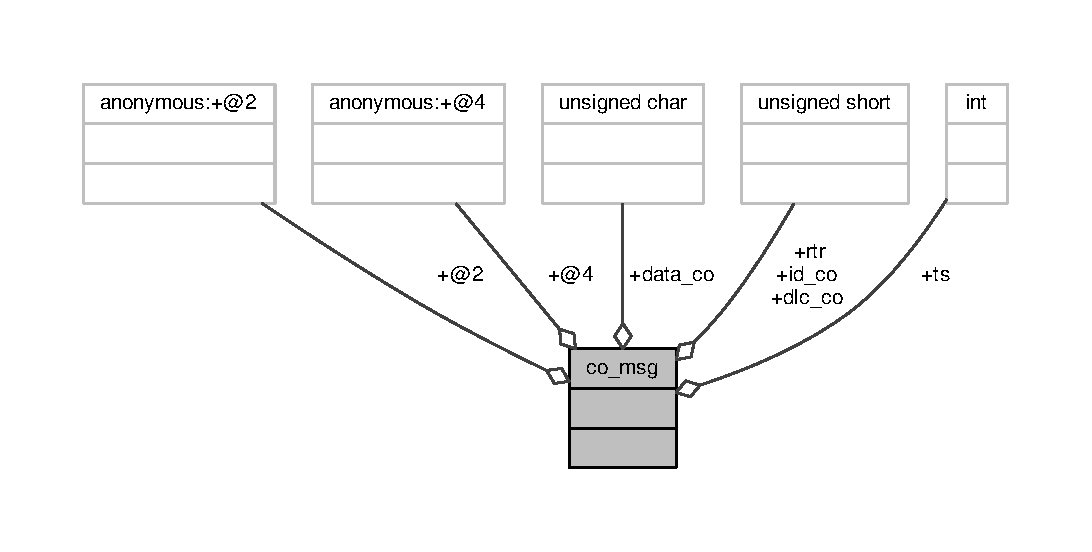
\includegraphics[width=350pt]{structco__msg__coll__graph}
\end{center}
\end{figure}
\subsection*{Public Attributes}
\begin{DoxyCompactItemize}
\item 
\begin{tabbing}
xx\=xx\=xx\=xx\=xx\=xx\=xx\=xx\=xx\=\kill
union \{\\
\>unsigned short \hyperlink{structco__msg_a634de83979d7da90565eccdf16304a07}{id\_co}\\
\}; \\

\end{tabbing}\item 
unsigned int \hyperlink{structco__msg_aaf8cd43d17baf495c982c87866fc90b2}{ts}
\item 
unsigned short \hyperlink{structco__msg_a4352880745fa6bc63d6c4e3c77870029}{rtr}\+:1
\item 
unsigned short \hyperlink{structco__msg_ab19d6996baf97d346427d9789d7e4a6b}{dlc\+\_\+co}
\item 
unsigned char \hyperlink{structco__msg_a3ced1bf4d72ca82fe53c829d42cd946e}{data\+\_\+co} \mbox{[}8\mbox{]}
\item 
\begin{tabbing}
xx\=xx\=xx\=xx\=xx\=xx\=xx\=xx\=xx\=\kill
union \{\\
\>unsigned short \hyperlink{structco__msg_a634de83979d7da90565eccdf16304a07}{id\_co}\\
\}; \\

\end{tabbing}\end{DoxyCompactItemize}


\subsection{Member Data Documentation}
\subsubsection[{\texorpdfstring{"@2}{@2}}]{\setlength{\rightskip}{0pt plus 5cm}union \{ ... \} }\hypertarget{structco__msg_af8251e2eaf9e807267d3ced55e292142}{}\label{structco__msg_af8251e2eaf9e807267d3ced55e292142}
\subsubsection[{\texorpdfstring{"@4}{@4}}]{\setlength{\rightskip}{0pt plus 5cm}union \{ ... \} }\hypertarget{structco__msg_a549464c55b7bbab6345f082dab73b275}{}\label{structco__msg_a549464c55b7bbab6345f082dab73b275}
\index{co\+\_\+msg@{co\+\_\+msg}!data\+\_\+co@{data\+\_\+co}}
\index{data\+\_\+co@{data\+\_\+co}!co\+\_\+msg@{co\+\_\+msg}}
\subsubsection[{\texorpdfstring{data\+\_\+co}{data_co}}]{\setlength{\rightskip}{0pt plus 5cm}unsigned char co\+\_\+msg\+::data\+\_\+co}\hypertarget{structco__msg_a3ced1bf4d72ca82fe53c829d42cd946e}{}\label{structco__msg_a3ced1bf4d72ca82fe53c829d42cd946e}
\index{co\+\_\+msg@{co\+\_\+msg}!dlc\+\_\+co@{dlc\+\_\+co}}
\index{dlc\+\_\+co@{dlc\+\_\+co}!co\+\_\+msg@{co\+\_\+msg}}
\subsubsection[{\texorpdfstring{dlc\+\_\+co}{dlc_co}}]{\setlength{\rightskip}{0pt plus 5cm}unsigned short co\+\_\+msg\+::dlc\+\_\+co}\hypertarget{structco__msg_ab19d6996baf97d346427d9789d7e4a6b}{}\label{structco__msg_ab19d6996baf97d346427d9789d7e4a6b}
\index{co\+\_\+msg@{co\+\_\+msg}!id\+\_\+co@{id\+\_\+co}}
\index{id\+\_\+co@{id\+\_\+co}!co\+\_\+msg@{co\+\_\+msg}}
\subsubsection[{\texorpdfstring{id\+\_\+co}{id_co}}]{\setlength{\rightskip}{0pt plus 5cm}unsigned short co\+\_\+msg\+::id\+\_\+co}\hypertarget{structco__msg_a634de83979d7da90565eccdf16304a07}{}\label{structco__msg_a634de83979d7da90565eccdf16304a07}
\index{co\+\_\+msg@{co\+\_\+msg}!rtr@{rtr}}
\index{rtr@{rtr}!co\+\_\+msg@{co\+\_\+msg}}
\subsubsection[{\texorpdfstring{rtr}{rtr}}]{\setlength{\rightskip}{0pt plus 5cm}unsigned short co\+\_\+msg\+::rtr}\hypertarget{structco__msg_a4352880745fa6bc63d6c4e3c77870029}{}\label{structco__msg_a4352880745fa6bc63d6c4e3c77870029}
\index{co\+\_\+msg@{co\+\_\+msg}!ts@{ts}}
\index{ts@{ts}!co\+\_\+msg@{co\+\_\+msg}}
\subsubsection[{\texorpdfstring{ts}{ts}}]{\setlength{\rightskip}{0pt plus 5cm}unsigned int co\+\_\+msg\+::ts}\hypertarget{structco__msg_aaf8cd43d17baf495c982c87866fc90b2}{}\label{structco__msg_aaf8cd43d17baf495c982c87866fc90b2}


The documentation for this struct was generated from the following files\+:\begin{DoxyCompactItemize}
\item 
\hyperlink{candatatypes_8h}{candatatypes.\+h}\item 
\hyperlink{co__msg_8h}{co\+\_\+msg.\+h}\end{DoxyCompactItemize}

\hypertarget{classDeviceChain}{}\section{Device\+Chain Class Reference}
\label{classDeviceChain}\index{Device\+Chain@{Device\+Chain}}


{\ttfamily \#include $<$Device\+Chain.\+h$>$}



Collaboration diagram for Device\+Chain\+:\nopagebreak
\begin{figure}[H]
\begin{center}
\leavevmode
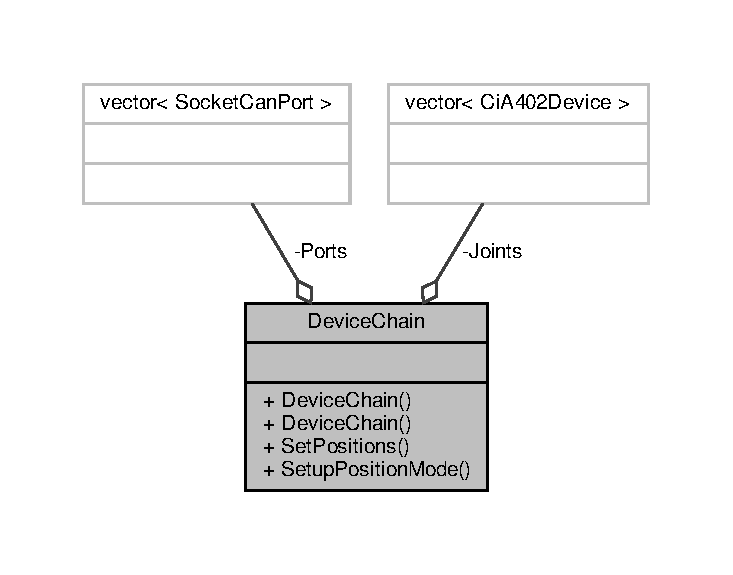
\includegraphics[width=350pt]{classDeviceChain__coll__graph}
\end{center}
\end{figure}
\subsection*{Public Member Functions}
\begin{DoxyCompactItemize}
\item 
\hyperlink{classDeviceChain_ad89af127eec501ad00ad5f5de197b21e}{Device\+Chain} (string actual\+Port)
\item 
\hyperlink{classDeviceChain_a20dd5853f160cfc8ef21ed93dac96f11}{Device\+Chain} (string actual\+Port, vector$<$ long $>$ ids)
\item 
long \hyperlink{classDeviceChain_ae6e9be5bfb46721d4c6b66d3d9541f25}{Set\+Positions} (vector$<$ double $>$ joint\+Angles)
\item 
long \hyperlink{classDeviceChain_a329b622f12a419f01a9bab38f869144b}{Setup\+Position\+Mode} (const uint32\+\_\+t velocity, const uint32\+\_\+t acceleration)
\end{DoxyCompactItemize}
\subsection*{Private Attributes}
\begin{DoxyCompactItemize}
\item 
std\+::vector$<$ \hyperlink{classCiA402Device}{Ci\+A402\+Device} $>$ \hyperlink{classDeviceChain_a114bea9dc1166ab2ea5a9ef7488c66ab}{Joints}
\item 
std\+::vector$<$ \hyperlink{classSocketCanPort}{Socket\+Can\+Port} $>$ \hyperlink{classDeviceChain_a760e12bf0095431fe76563cc5d7969de}{Ports}
\end{DoxyCompactItemize}


\subsection{Constructor \& Destructor Documentation}
\mbox{\Hypertarget{classDeviceChain_ad89af127eec501ad00ad5f5de197b21e}\label{classDeviceChain_ad89af127eec501ad00ad5f5de197b21e}} 
\index{Device\+Chain@{Device\+Chain}!Device\+Chain@{Device\+Chain}}
\index{Device\+Chain@{Device\+Chain}!Device\+Chain@{Device\+Chain}}
\subsubsection{\texorpdfstring{Device\+Chain()}{DeviceChain()}\hspace{0.1cm}{\footnotesize\ttfamily [1/2]}}
{\footnotesize\ttfamily Device\+Chain\+::\+Device\+Chain (\begin{DoxyParamCaption}\item[{string}]{actual\+Port }\end{DoxyParamCaption})}

\mbox{\Hypertarget{classDeviceChain_a20dd5853f160cfc8ef21ed93dac96f11}\label{classDeviceChain_a20dd5853f160cfc8ef21ed93dac96f11}} 
\index{Device\+Chain@{Device\+Chain}!Device\+Chain@{Device\+Chain}}
\index{Device\+Chain@{Device\+Chain}!Device\+Chain@{Device\+Chain}}
\subsubsection{\texorpdfstring{Device\+Chain()}{DeviceChain()}\hspace{0.1cm}{\footnotesize\ttfamily [2/2]}}
{\footnotesize\ttfamily Device\+Chain\+::\+Device\+Chain (\begin{DoxyParamCaption}\item[{string}]{actual\+Port,  }\item[{vector$<$ long $>$}]{ids }\end{DoxyParamCaption})}



\subsection{Member Function Documentation}
\mbox{\Hypertarget{classDeviceChain_ae6e9be5bfb46721d4c6b66d3d9541f25}\label{classDeviceChain_ae6e9be5bfb46721d4c6b66d3d9541f25}} 
\index{Device\+Chain@{Device\+Chain}!Set\+Positions@{Set\+Positions}}
\index{Set\+Positions@{Set\+Positions}!Device\+Chain@{Device\+Chain}}
\subsubsection{\texorpdfstring{Set\+Positions()}{SetPositions()}}
{\footnotesize\ttfamily long Device\+Chain\+::\+Set\+Positions (\begin{DoxyParamCaption}\item[{vector$<$ double $>$}]{joint\+Angles }\end{DoxyParamCaption})}

\mbox{\Hypertarget{classDeviceChain_a329b622f12a419f01a9bab38f869144b}\label{classDeviceChain_a329b622f12a419f01a9bab38f869144b}} 
\index{Device\+Chain@{Device\+Chain}!Setup\+Position\+Mode@{Setup\+Position\+Mode}}
\index{Setup\+Position\+Mode@{Setup\+Position\+Mode}!Device\+Chain@{Device\+Chain}}
\subsubsection{\texorpdfstring{Setup\+Position\+Mode()}{SetupPositionMode()}}
{\footnotesize\ttfamily long Device\+Chain\+::\+Setup\+Position\+Mode (\begin{DoxyParamCaption}\item[{const uint32\+\_\+t}]{velocity,  }\item[{const uint32\+\_\+t}]{acceleration }\end{DoxyParamCaption})}



\subsection{Member Data Documentation}
\mbox{\Hypertarget{classDeviceChain_a114bea9dc1166ab2ea5a9ef7488c66ab}\label{classDeviceChain_a114bea9dc1166ab2ea5a9ef7488c66ab}} 
\index{Device\+Chain@{Device\+Chain}!Joints@{Joints}}
\index{Joints@{Joints}!Device\+Chain@{Device\+Chain}}
\subsubsection{\texorpdfstring{Joints}{Joints}}
{\footnotesize\ttfamily std\+::vector$<$\hyperlink{classCiA402Device}{Ci\+A402\+Device}$>$ Device\+Chain\+::\+Joints\hspace{0.3cm}{\ttfamily [private]}}

\mbox{\Hypertarget{classDeviceChain_a760e12bf0095431fe76563cc5d7969de}\label{classDeviceChain_a760e12bf0095431fe76563cc5d7969de}} 
\index{Device\+Chain@{Device\+Chain}!Ports@{Ports}}
\index{Ports@{Ports}!Device\+Chain@{Device\+Chain}}
\subsubsection{\texorpdfstring{Ports}{Ports}}
{\footnotesize\ttfamily std\+::vector$<$\hyperlink{classSocketCanPort}{Socket\+Can\+Port}$>$ Device\+Chain\+::\+Ports\hspace{0.3cm}{\ttfamily [private]}}



The documentation for this class was generated from the following files\+:\begin{DoxyCompactItemize}
\item 
\hyperlink{DeviceChain_8h}{Device\+Chain.\+h}\item 
\hyperlink{DeviceChain_8cpp}{Device\+Chain.\+cpp}\end{DoxyCompactItemize}

\hypertarget{structerr__stat}{}\section{err\+\_\+stat Struct Reference}
\label{structerr__stat}\index{err\+\_\+stat@{err\+\_\+stat}}


{\ttfamily \#include $<$hico\+\_\+api.\+h$>$}



Collaboration diagram for err\+\_\+stat\+:\nopagebreak
\begin{figure}[H]
\begin{center}
\leavevmode
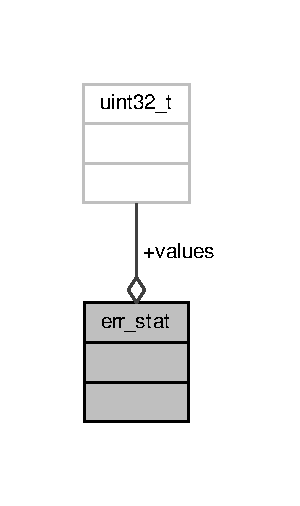
\includegraphics[width=144pt]{structerr__stat__coll__graph}
\end{center}
\end{figure}
\subsection*{Public Attributes}
\begin{DoxyCompactItemize}
\item 
uint32\+\_\+t \hyperlink{structerr__stat_a659e627af5963248da109c8e2404cd08}{values} \mbox{[}0x3f\mbox{]}
\end{DoxyCompactItemize}


\subsection{Member Data Documentation}
\index{err\+\_\+stat@{err\+\_\+stat}!values@{values}}
\index{values@{values}!err\+\_\+stat@{err\+\_\+stat}}
\subsubsection[{\texorpdfstring{values}{values}}]{\setlength{\rightskip}{0pt plus 5cm}uint32\+\_\+t err\+\_\+stat\+::values\mbox{[}0x3f\mbox{]}}\hypertarget{structerr__stat_a659e627af5963248da109c8e2404cd08}{}\label{structerr__stat_a659e627af5963248da109c8e2404cd08}


The documentation for this struct was generated from the following file\+:\begin{DoxyCompactItemize}
\item 
\hyperlink{hico__api_8h}{hico\+\_\+api.\+h}\end{DoxyCompactItemize}

\hypertarget{classPortBase}{}\section{Port\+Base Class Reference}
\label{classPortBase}\index{Port\+Base@{Port\+Base}}


{\ttfamily \#include $<$Port\+Base.\+h$>$}



Inheritance diagram for Port\+Base\+:
\nopagebreak
\begin{figure}[H]
\begin{center}
\leavevmode
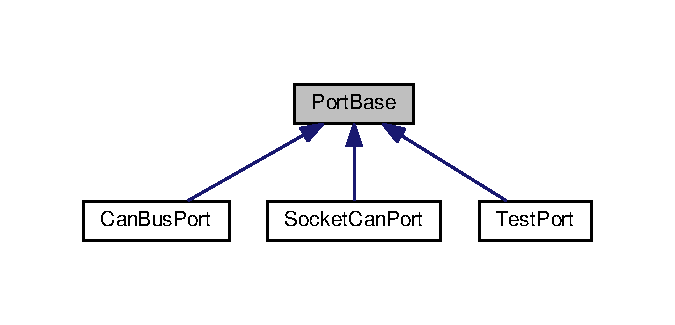
\includegraphics[width=350pt]{classPortBase__inherit__graph}
\end{center}
\end{figure}


Collaboration diagram for Port\+Base\+:
\nopagebreak
\begin{figure}[H]
\begin{center}
\leavevmode
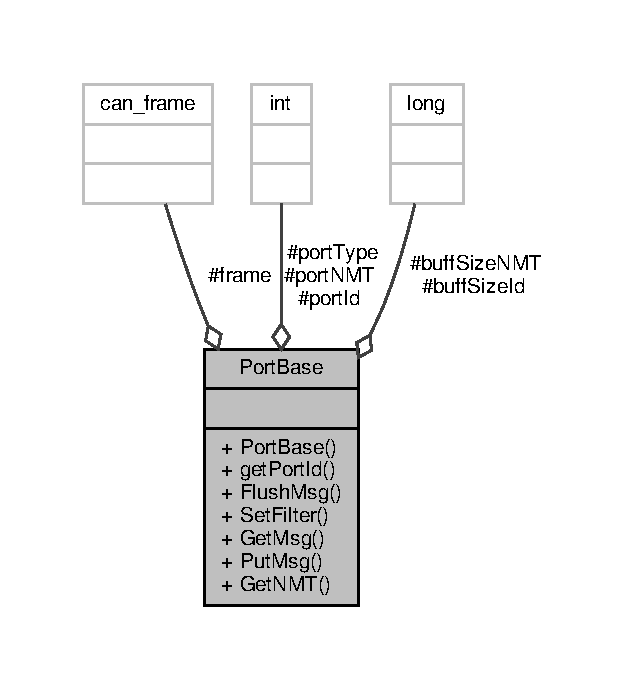
\includegraphics[width=301pt]{classPortBase__coll__graph}
\end{center}
\end{figure}
\subsection*{Public Member Functions}
\begin{DoxyCompactItemize}
\item 
\hyperlink{classPortBase_acb7872550bc94538ef95d2510d763be3}{Port\+Base} ()
\item 
int \hyperlink{classPortBase_a45ec4a2cd5e17e098f6f72677437f066}{get\+Port\+Id} ()
\item 
long \hyperlink{classPortBase_a913932fc850e9aebc947542773c669ad}{Flush\+Msg} ()
\item 
virtual long \hyperlink{classPortBase_a1d857a81a8e3f3bd460ef7c802ee762c}{Set\+Filter} (uint32\+\_\+t can\+Id, uint32\+\_\+t mask)=0
\item 
virtual long \hyperlink{classPortBase_a4fe82768f2b79889d7084292ac0e8696}{Get\+Msg} (uint32\+\_\+t \&can\+Id, uint8\+\_\+t $\ast$data, uint8\+\_\+t \&size)=0
\item 
virtual long \hyperlink{classPortBase_a26213ebb6ea0a0b77f60c28944e3bb8e}{Put\+Msg} (const uint32\+\_\+t \&can\+Id, uint8\+\_\+t $\ast$const data, const uint8\+\_\+t size)=0
\item 
virtual long \hyperlink{classPortBase_abab2bf17b01d87c2bca01cb2151aa2f1}{Get\+N\+MT} (uint8\+\_\+t $\ast$data, uint8\+\_\+t \&size)=0
\end{DoxyCompactItemize}
\subsection*{Protected Attributes}
\begin{DoxyCompactItemize}
\item 
int \hyperlink{classPortBase_af8816a6f73bf391d2948f3564f8ea1df}{port\+Id}
\item 
int \hyperlink{classPortBase_a6f18d480ef41a91fd2957927fe94c408}{port\+Type}
\item 
int \hyperlink{classPortBase_ae63f6df54bbeac1046b5dfbe178e1cee}{port\+N\+MT}
\item 
can\+\_\+frame \hyperlink{classPortBase_ae175156fa18f3be1820adea89ef7b13c}{frame}
\item 
long \hyperlink{classPortBase_a559431268076ea9b23bce545510f7b39}{buff\+Size\+Id}
\item 
long \hyperlink{classPortBase_aba8241e5d55c06c7d1a11ebb18096328}{buff\+Size\+N\+MT}
\end{DoxyCompactItemize}


\subsection{Constructor \& Destructor Documentation}
\index{Port\+Base@{Port\+Base}!Port\+Base@{Port\+Base}}
\index{Port\+Base@{Port\+Base}!Port\+Base@{Port\+Base}}
\subsubsection[{\texorpdfstring{Port\+Base()}{PortBase()}}]{\setlength{\rightskip}{0pt plus 5cm}Port\+Base\+::\+Port\+Base (
\begin{DoxyParamCaption}
{}
\end{DoxyParamCaption}
)}\hypertarget{classPortBase_acb7872550bc94538ef95d2510d763be3}{}\label{classPortBase_acb7872550bc94538ef95d2510d763be3}


\subsection{Member Function Documentation}
\index{Port\+Base@{Port\+Base}!Flush\+Msg@{Flush\+Msg}}
\index{Flush\+Msg@{Flush\+Msg}!Port\+Base@{Port\+Base}}
\subsubsection[{\texorpdfstring{Flush\+Msg()}{FlushMsg()}}]{\setlength{\rightskip}{0pt plus 5cm}long Port\+Base\+::\+Flush\+Msg (
\begin{DoxyParamCaption}
{}
\end{DoxyParamCaption}
)}\hypertarget{classPortBase_a913932fc850e9aebc947542773c669ad}{}\label{classPortBase_a913932fc850e9aebc947542773c669ad}
\index{Port\+Base@{Port\+Base}!Get\+Msg@{Get\+Msg}}
\index{Get\+Msg@{Get\+Msg}!Port\+Base@{Port\+Base}}
\subsubsection[{\texorpdfstring{Get\+Msg(uint32\+\_\+t \&can\+Id, uint8\+\_\+t $\ast$data, uint8\+\_\+t \&size)=0}{GetMsg(uint32_t &canId, uint8_t *data, uint8_t &size)=0}}]{\setlength{\rightskip}{0pt plus 5cm}virtual long Port\+Base\+::\+Get\+Msg (
\begin{DoxyParamCaption}
\item[{uint32\+\_\+t \&}]{can\+Id, }
\item[{uint8\+\_\+t $\ast$}]{data, }
\item[{uint8\+\_\+t \&}]{size}
\end{DoxyParamCaption}
)\hspace{0.3cm}{\ttfamily [pure virtual]}}\hypertarget{classPortBase_a4fe82768f2b79889d7084292ac0e8696}{}\label{classPortBase_a4fe82768f2b79889d7084292ac0e8696}


Implemented in \hyperlink{classCanBusPort_ac442e4e5b7bb154ea6322518b715f406}{Can\+Bus\+Port}, and \hyperlink{classSocketCanPort_aa9684efc602da057cb4928d52395af33}{Socket\+Can\+Port}.

\index{Port\+Base@{Port\+Base}!Get\+N\+MT@{Get\+N\+MT}}
\index{Get\+N\+MT@{Get\+N\+MT}!Port\+Base@{Port\+Base}}
\subsubsection[{\texorpdfstring{Get\+N\+M\+T(uint8\+\_\+t $\ast$data, uint8\+\_\+t \&size)=0}{GetNMT(uint8_t *data, uint8_t &size)=0}}]{\setlength{\rightskip}{0pt plus 5cm}virtual long Port\+Base\+::\+Get\+N\+MT (
\begin{DoxyParamCaption}
\item[{uint8\+\_\+t $\ast$}]{data, }
\item[{uint8\+\_\+t \&}]{size}
\end{DoxyParamCaption}
)\hspace{0.3cm}{\ttfamily [pure virtual]}}\hypertarget{classPortBase_abab2bf17b01d87c2bca01cb2151aa2f1}{}\label{classPortBase_abab2bf17b01d87c2bca01cb2151aa2f1}


Implemented in \hyperlink{classCanBusPort_a41242dc7980ca398e4770813e50ef32b}{Can\+Bus\+Port}, and \hyperlink{classSocketCanPort_a2efe27bd3bb8c8127c89925e1e21535a}{Socket\+Can\+Port}.

\index{Port\+Base@{Port\+Base}!get\+Port\+Id@{get\+Port\+Id}}
\index{get\+Port\+Id@{get\+Port\+Id}!Port\+Base@{Port\+Base}}
\subsubsection[{\texorpdfstring{get\+Port\+Id()}{getPortId()}}]{\setlength{\rightskip}{0pt plus 5cm}int Port\+Base\+::get\+Port\+Id (
\begin{DoxyParamCaption}
{}
\end{DoxyParamCaption}
)}\hypertarget{classPortBase_a45ec4a2cd5e17e098f6f72677437f066}{}\label{classPortBase_a45ec4a2cd5e17e098f6f72677437f066}
\index{Port\+Base@{Port\+Base}!Put\+Msg@{Put\+Msg}}
\index{Put\+Msg@{Put\+Msg}!Port\+Base@{Port\+Base}}
\subsubsection[{\texorpdfstring{Put\+Msg(const uint32\+\_\+t \&can\+Id, uint8\+\_\+t $\ast$const data, const uint8\+\_\+t size)=0}{PutMsg(const uint32_t &canId, uint8_t *const data, const uint8_t size)=0}}]{\setlength{\rightskip}{0pt plus 5cm}virtual long Port\+Base\+::\+Put\+Msg (
\begin{DoxyParamCaption}
\item[{const uint32\+\_\+t \&}]{can\+Id, }
\item[{uint8\+\_\+t $\ast$const}]{data, }
\item[{const uint8\+\_\+t}]{size}
\end{DoxyParamCaption}
)\hspace{0.3cm}{\ttfamily [pure virtual]}}\hypertarget{classPortBase_a26213ebb6ea0a0b77f60c28944e3bb8e}{}\label{classPortBase_a26213ebb6ea0a0b77f60c28944e3bb8e}


Implemented in \hyperlink{classCanBusPort_a2bb802ad7a14e260f0f51b79d4c53c43}{Can\+Bus\+Port}, and \hyperlink{classSocketCanPort_a9375a0c1e33978c83ebd188100898633}{Socket\+Can\+Port}.

\index{Port\+Base@{Port\+Base}!Set\+Filter@{Set\+Filter}}
\index{Set\+Filter@{Set\+Filter}!Port\+Base@{Port\+Base}}
\subsubsection[{\texorpdfstring{Set\+Filter(uint32\+\_\+t can\+Id, uint32\+\_\+t mask)=0}{SetFilter(uint32_t canId, uint32_t mask)=0}}]{\setlength{\rightskip}{0pt plus 5cm}virtual long Port\+Base\+::\+Set\+Filter (
\begin{DoxyParamCaption}
\item[{uint32\+\_\+t}]{can\+Id, }
\item[{uint32\+\_\+t}]{mask}
\end{DoxyParamCaption}
)\hspace{0.3cm}{\ttfamily [pure virtual]}}\hypertarget{classPortBase_a1d857a81a8e3f3bd460ef7c802ee762c}{}\label{classPortBase_a1d857a81a8e3f3bd460ef7c802ee762c}


Implemented in \hyperlink{classCanBusPort_af09c794e3af86e89c8a511535f856dc9}{Can\+Bus\+Port}, and \hyperlink{classSocketCanPort_a1a5d0866524dae11ddff0d1ac22e0dd5}{Socket\+Can\+Port}.



\subsection{Member Data Documentation}
\index{Port\+Base@{Port\+Base}!buff\+Size\+Id@{buff\+Size\+Id}}
\index{buff\+Size\+Id@{buff\+Size\+Id}!Port\+Base@{Port\+Base}}
\subsubsection[{\texorpdfstring{buff\+Size\+Id}{buffSizeId}}]{\setlength{\rightskip}{0pt plus 5cm}long Port\+Base\+::buff\+Size\+Id\hspace{0.3cm}{\ttfamily [protected]}}\hypertarget{classPortBase_a559431268076ea9b23bce545510f7b39}{}\label{classPortBase_a559431268076ea9b23bce545510f7b39}
\index{Port\+Base@{Port\+Base}!buff\+Size\+N\+MT@{buff\+Size\+N\+MT}}
\index{buff\+Size\+N\+MT@{buff\+Size\+N\+MT}!Port\+Base@{Port\+Base}}
\subsubsection[{\texorpdfstring{buff\+Size\+N\+MT}{buffSizeNMT}}]{\setlength{\rightskip}{0pt plus 5cm}long Port\+Base\+::buff\+Size\+N\+MT\hspace{0.3cm}{\ttfamily [protected]}}\hypertarget{classPortBase_aba8241e5d55c06c7d1a11ebb18096328}{}\label{classPortBase_aba8241e5d55c06c7d1a11ebb18096328}
\index{Port\+Base@{Port\+Base}!frame@{frame}}
\index{frame@{frame}!Port\+Base@{Port\+Base}}
\subsubsection[{\texorpdfstring{frame}{frame}}]{\setlength{\rightskip}{0pt plus 5cm}can\+\_\+frame Port\+Base\+::frame\hspace{0.3cm}{\ttfamily [protected]}}\hypertarget{classPortBase_ae175156fa18f3be1820adea89ef7b13c}{}\label{classPortBase_ae175156fa18f3be1820adea89ef7b13c}
\index{Port\+Base@{Port\+Base}!port\+Id@{port\+Id}}
\index{port\+Id@{port\+Id}!Port\+Base@{Port\+Base}}
\subsubsection[{\texorpdfstring{port\+Id}{portId}}]{\setlength{\rightskip}{0pt plus 5cm}int Port\+Base\+::port\+Id\hspace{0.3cm}{\ttfamily [protected]}}\hypertarget{classPortBase_af8816a6f73bf391d2948f3564f8ea1df}{}\label{classPortBase_af8816a6f73bf391d2948f3564f8ea1df}
\index{Port\+Base@{Port\+Base}!port\+N\+MT@{port\+N\+MT}}
\index{port\+N\+MT@{port\+N\+MT}!Port\+Base@{Port\+Base}}
\subsubsection[{\texorpdfstring{port\+N\+MT}{portNMT}}]{\setlength{\rightskip}{0pt plus 5cm}int Port\+Base\+::port\+N\+MT\hspace{0.3cm}{\ttfamily [protected]}}\hypertarget{classPortBase_ae63f6df54bbeac1046b5dfbe178e1cee}{}\label{classPortBase_ae63f6df54bbeac1046b5dfbe178e1cee}
\index{Port\+Base@{Port\+Base}!port\+Type@{port\+Type}}
\index{port\+Type@{port\+Type}!Port\+Base@{Port\+Base}}
\subsubsection[{\texorpdfstring{port\+Type}{portType}}]{\setlength{\rightskip}{0pt plus 5cm}int Port\+Base\+::port\+Type\hspace{0.3cm}{\ttfamily [protected]}}\hypertarget{classPortBase_a6f18d480ef41a91fd2957927fe94c408}{}\label{classPortBase_a6f18d480ef41a91fd2957927fe94c408}


The documentation for this class was generated from the following files\+:\begin{DoxyCompactItemize}
\item 
\hyperlink{PortBase_8h}{Port\+Base.\+h}\item 
\hyperlink{PortBase_8cpp}{Port\+Base.\+cpp}\end{DoxyCompactItemize}

\hypertarget{classSocketCanPort}{}\section{Socket\+Can\+Port Class Reference}
\label{classSocketCanPort}\index{Socket\+Can\+Port@{Socket\+Can\+Port}}


{\ttfamily \#include $<$Socket\+Can\+Port.\+h$>$}



Inheritance diagram for Socket\+Can\+Port\+:
\nopagebreak
\begin{figure}[H]
\begin{center}
\leavevmode
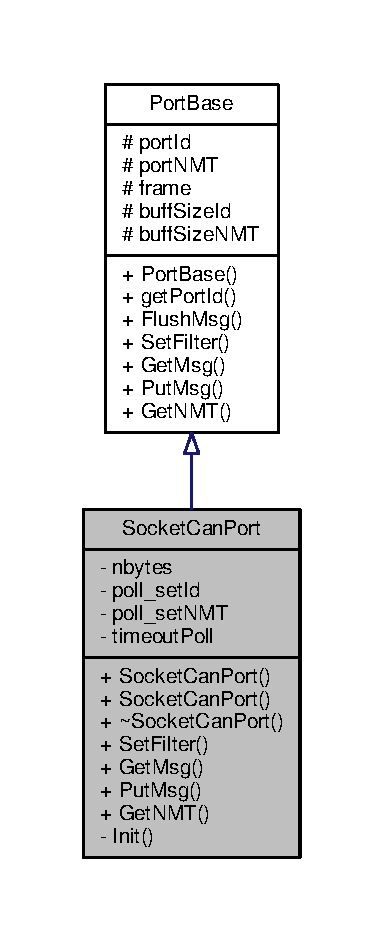
\includegraphics[width=184pt]{classSocketCanPort__inherit__graph}
\end{center}
\end{figure}


Collaboration diagram for Socket\+Can\+Port\+:
\nopagebreak
\begin{figure}[H]
\begin{center}
\leavevmode
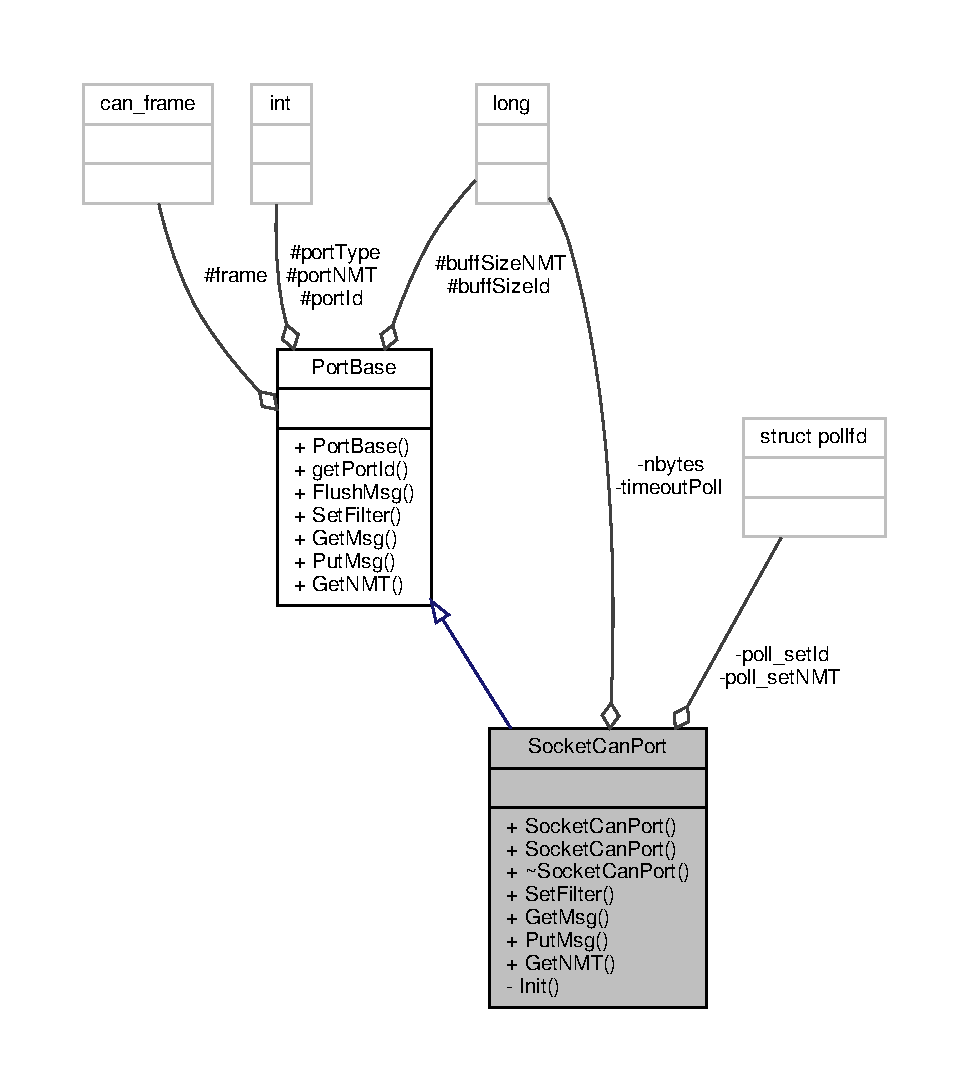
\includegraphics[width=350pt]{classSocketCanPort__coll__graph}
\end{center}
\end{figure}
\subsection*{Public Member Functions}
\begin{DoxyCompactItemize}
\item 
\hyperlink{classSocketCanPort_af3593609acea236b10646732e277837f}{Socket\+Can\+Port} ()
\item 
\hyperlink{classSocketCanPort_a087bc07f3c1658e3cb994d85fcb3da5e}{Socket\+Can\+Port} (string can\+Port)
\item 
\hyperlink{classSocketCanPort_a0d004347e49110daa1ee29e1d1bc85c0}{$\sim$\+Socket\+Can\+Port} ()
\item 
long \hyperlink{classSocketCanPort_a1a5d0866524dae11ddff0d1ac22e0dd5}{Set\+Filter} (uint32\+\_\+t can\+Id, uint32\+\_\+t mask)
\item 
long \hyperlink{classSocketCanPort_aa9684efc602da057cb4928d52395af33}{Get\+Msg} (uint32\+\_\+t \&can\+Id, uint8\+\_\+t $\ast$data, uint8\+\_\+t \&size)
\item 
long \hyperlink{classSocketCanPort_a9375a0c1e33978c83ebd188100898633}{Put\+Msg} (const uint32\+\_\+t \&can\+Id, uint8\+\_\+t $\ast$const data, const uint8\+\_\+t size)
\item 
long \hyperlink{classSocketCanPort_a2efe27bd3bb8c8127c89925e1e21535a}{Get\+N\+MT} (uint8\+\_\+t $\ast$data, uint8\+\_\+t \&size)
\end{DoxyCompactItemize}
\subsection*{Private Member Functions}
\begin{DoxyCompactItemize}
\item 
long \hyperlink{classSocketCanPort_a9209d295c98c12ab85ec61773b775bf4}{Init} (string can\+Port)
\end{DoxyCompactItemize}
\subsection*{Private Attributes}
\begin{DoxyCompactItemize}
\item 
long \hyperlink{classSocketCanPort_a7b06b4d8c897c1a189329f20632fdb71}{nbytes}
\item 
struct pollfd \hyperlink{classSocketCanPort_ad0374fe5ea78a061e7abd16b812f44d5}{poll\+\_\+set\+Id} \mbox{[}1\mbox{]}
\item 
struct pollfd \hyperlink{classSocketCanPort_afaaf9cd49684de93be7370988ec64b47}{poll\+\_\+set\+N\+MT} \mbox{[}1\mbox{]}
\item 
long \hyperlink{classSocketCanPort_a18e670bf7f98482e022da2fd11264309}{timeout\+Poll}
\end{DoxyCompactItemize}
\subsection*{Additional Inherited Members}


\subsection{Constructor \& Destructor Documentation}
\index{Socket\+Can\+Port@{Socket\+Can\+Port}!Socket\+Can\+Port@{Socket\+Can\+Port}}
\index{Socket\+Can\+Port@{Socket\+Can\+Port}!Socket\+Can\+Port@{Socket\+Can\+Port}}
\subsubsection[{\texorpdfstring{Socket\+Can\+Port()}{SocketCanPort()}}]{\setlength{\rightskip}{0pt plus 5cm}Socket\+Can\+Port\+::\+Socket\+Can\+Port (
\begin{DoxyParamCaption}
{}
\end{DoxyParamCaption}
)}\hypertarget{classSocketCanPort_af3593609acea236b10646732e277837f}{}\label{classSocketCanPort_af3593609acea236b10646732e277837f}
\index{Socket\+Can\+Port@{Socket\+Can\+Port}!Socket\+Can\+Port@{Socket\+Can\+Port}}
\index{Socket\+Can\+Port@{Socket\+Can\+Port}!Socket\+Can\+Port@{Socket\+Can\+Port}}
\subsubsection[{\texorpdfstring{Socket\+Can\+Port(string can\+Port)}{SocketCanPort(string canPort)}}]{\setlength{\rightskip}{0pt plus 5cm}Socket\+Can\+Port\+::\+Socket\+Can\+Port (
\begin{DoxyParamCaption}
\item[{string}]{can\+Port}
\end{DoxyParamCaption}
)}\hypertarget{classSocketCanPort_a087bc07f3c1658e3cb994d85fcb3da5e}{}\label{classSocketCanPort_a087bc07f3c1658e3cb994d85fcb3da5e}
\index{Socket\+Can\+Port@{Socket\+Can\+Port}!````~Socket\+Can\+Port@{$\sim$\+Socket\+Can\+Port}}
\index{````~Socket\+Can\+Port@{$\sim$\+Socket\+Can\+Port}!Socket\+Can\+Port@{Socket\+Can\+Port}}
\subsubsection[{\texorpdfstring{$\sim$\+Socket\+Can\+Port()}{~SocketCanPort()}}]{\setlength{\rightskip}{0pt plus 5cm}Socket\+Can\+Port\+::$\sim$\+Socket\+Can\+Port (
\begin{DoxyParamCaption}
{}
\end{DoxyParamCaption}
)}\hypertarget{classSocketCanPort_a0d004347e49110daa1ee29e1d1bc85c0}{}\label{classSocketCanPort_a0d004347e49110daa1ee29e1d1bc85c0}


\subsection{Member Function Documentation}
\index{Socket\+Can\+Port@{Socket\+Can\+Port}!Get\+Msg@{Get\+Msg}}
\index{Get\+Msg@{Get\+Msg}!Socket\+Can\+Port@{Socket\+Can\+Port}}
\subsubsection[{\texorpdfstring{Get\+Msg(uint32\+\_\+t \&can\+Id, uint8\+\_\+t $\ast$data, uint8\+\_\+t \&size)}{GetMsg(uint32_t &canId, uint8_t *data, uint8_t &size)}}]{\setlength{\rightskip}{0pt plus 5cm}long Socket\+Can\+Port\+::\+Get\+Msg (
\begin{DoxyParamCaption}
\item[{uint32\+\_\+t \&}]{can\+Id, }
\item[{uint8\+\_\+t $\ast$}]{data, }
\item[{uint8\+\_\+t \&}]{size}
\end{DoxyParamCaption}
)\hspace{0.3cm}{\ttfamily [virtual]}}\hypertarget{classSocketCanPort_aa9684efc602da057cb4928d52395af33}{}\label{classSocketCanPort_aa9684efc602da057cb4928d52395af33}


Implements \hyperlink{classPortBase_a4fe82768f2b79889d7084292ac0e8696}{Port\+Base}.

\index{Socket\+Can\+Port@{Socket\+Can\+Port}!Get\+N\+MT@{Get\+N\+MT}}
\index{Get\+N\+MT@{Get\+N\+MT}!Socket\+Can\+Port@{Socket\+Can\+Port}}
\subsubsection[{\texorpdfstring{Get\+N\+M\+T(uint8\+\_\+t $\ast$data, uint8\+\_\+t \&size)}{GetNMT(uint8_t *data, uint8_t &size)}}]{\setlength{\rightskip}{0pt plus 5cm}long Socket\+Can\+Port\+::\+Get\+N\+MT (
\begin{DoxyParamCaption}
\item[{uint8\+\_\+t $\ast$}]{data, }
\item[{uint8\+\_\+t \&}]{size}
\end{DoxyParamCaption}
)\hspace{0.3cm}{\ttfamily [virtual]}}\hypertarget{classSocketCanPort_a2efe27bd3bb8c8127c89925e1e21535a}{}\label{classSocketCanPort_a2efe27bd3bb8c8127c89925e1e21535a}


Implements \hyperlink{classPortBase_abab2bf17b01d87c2bca01cb2151aa2f1}{Port\+Base}.

\index{Socket\+Can\+Port@{Socket\+Can\+Port}!Init@{Init}}
\index{Init@{Init}!Socket\+Can\+Port@{Socket\+Can\+Port}}
\subsubsection[{\texorpdfstring{Init(string can\+Port)}{Init(string canPort)}}]{\setlength{\rightskip}{0pt plus 5cm}long Socket\+Can\+Port\+::\+Init (
\begin{DoxyParamCaption}
\item[{string}]{can\+Port}
\end{DoxyParamCaption}
)\hspace{0.3cm}{\ttfamily [private]}}\hypertarget{classSocketCanPort_a9209d295c98c12ab85ec61773b775bf4}{}\label{classSocketCanPort_a9209d295c98c12ab85ec61773b775bf4}
\index{Socket\+Can\+Port@{Socket\+Can\+Port}!Put\+Msg@{Put\+Msg}}
\index{Put\+Msg@{Put\+Msg}!Socket\+Can\+Port@{Socket\+Can\+Port}}
\subsubsection[{\texorpdfstring{Put\+Msg(const uint32\+\_\+t \&can\+Id, uint8\+\_\+t $\ast$const data, const uint8\+\_\+t size)}{PutMsg(const uint32_t &canId, uint8_t *const data, const uint8_t size)}}]{\setlength{\rightskip}{0pt plus 5cm}long Socket\+Can\+Port\+::\+Put\+Msg (
\begin{DoxyParamCaption}
\item[{const uint32\+\_\+t \&}]{can\+Id, }
\item[{uint8\+\_\+t $\ast$const}]{data, }
\item[{const uint8\+\_\+t}]{size}
\end{DoxyParamCaption}
)\hspace{0.3cm}{\ttfamily [virtual]}}\hypertarget{classSocketCanPort_a9375a0c1e33978c83ebd188100898633}{}\label{classSocketCanPort_a9375a0c1e33978c83ebd188100898633}


Implements \hyperlink{classPortBase_a26213ebb6ea0a0b77f60c28944e3bb8e}{Port\+Base}.

\index{Socket\+Can\+Port@{Socket\+Can\+Port}!Set\+Filter@{Set\+Filter}}
\index{Set\+Filter@{Set\+Filter}!Socket\+Can\+Port@{Socket\+Can\+Port}}
\subsubsection[{\texorpdfstring{Set\+Filter(uint32\+\_\+t can\+Id, uint32\+\_\+t mask)}{SetFilter(uint32_t canId, uint32_t mask)}}]{\setlength{\rightskip}{0pt plus 5cm}long Socket\+Can\+Port\+::\+Set\+Filter (
\begin{DoxyParamCaption}
\item[{uint32\+\_\+t}]{can\+Id, }
\item[{uint32\+\_\+t}]{mask}
\end{DoxyParamCaption}
)\hspace{0.3cm}{\ttfamily [virtual]}}\hypertarget{classSocketCanPort_a1a5d0866524dae11ddff0d1ac22e0dd5}{}\label{classSocketCanPort_a1a5d0866524dae11ddff0d1ac22e0dd5}


Implements \hyperlink{classPortBase_a1d857a81a8e3f3bd460ef7c802ee762c}{Port\+Base}.



\subsection{Member Data Documentation}
\index{Socket\+Can\+Port@{Socket\+Can\+Port}!nbytes@{nbytes}}
\index{nbytes@{nbytes}!Socket\+Can\+Port@{Socket\+Can\+Port}}
\subsubsection[{\texorpdfstring{nbytes}{nbytes}}]{\setlength{\rightskip}{0pt plus 5cm}long Socket\+Can\+Port\+::nbytes\hspace{0.3cm}{\ttfamily [private]}}\hypertarget{classSocketCanPort_a7b06b4d8c897c1a189329f20632fdb71}{}\label{classSocketCanPort_a7b06b4d8c897c1a189329f20632fdb71}
\index{Socket\+Can\+Port@{Socket\+Can\+Port}!poll\+\_\+set\+Id@{poll\+\_\+set\+Id}}
\index{poll\+\_\+set\+Id@{poll\+\_\+set\+Id}!Socket\+Can\+Port@{Socket\+Can\+Port}}
\subsubsection[{\texorpdfstring{poll\+\_\+set\+Id}{poll_setId}}]{\setlength{\rightskip}{0pt plus 5cm}struct pollfd Socket\+Can\+Port\+::poll\+\_\+set\+Id\mbox{[}1\mbox{]}\hspace{0.3cm}{\ttfamily [private]}}\hypertarget{classSocketCanPort_ad0374fe5ea78a061e7abd16b812f44d5}{}\label{classSocketCanPort_ad0374fe5ea78a061e7abd16b812f44d5}
\index{Socket\+Can\+Port@{Socket\+Can\+Port}!poll\+\_\+set\+N\+MT@{poll\+\_\+set\+N\+MT}}
\index{poll\+\_\+set\+N\+MT@{poll\+\_\+set\+N\+MT}!Socket\+Can\+Port@{Socket\+Can\+Port}}
\subsubsection[{\texorpdfstring{poll\+\_\+set\+N\+MT}{poll_setNMT}}]{\setlength{\rightskip}{0pt plus 5cm}struct pollfd Socket\+Can\+Port\+::poll\+\_\+set\+N\+MT\mbox{[}1\mbox{]}\hspace{0.3cm}{\ttfamily [private]}}\hypertarget{classSocketCanPort_afaaf9cd49684de93be7370988ec64b47}{}\label{classSocketCanPort_afaaf9cd49684de93be7370988ec64b47}
\index{Socket\+Can\+Port@{Socket\+Can\+Port}!timeout\+Poll@{timeout\+Poll}}
\index{timeout\+Poll@{timeout\+Poll}!Socket\+Can\+Port@{Socket\+Can\+Port}}
\subsubsection[{\texorpdfstring{timeout\+Poll}{timeoutPoll}}]{\setlength{\rightskip}{0pt plus 5cm}long Socket\+Can\+Port\+::timeout\+Poll\hspace{0.3cm}{\ttfamily [private]}}\hypertarget{classSocketCanPort_a18e670bf7f98482e022da2fd11264309}{}\label{classSocketCanPort_a18e670bf7f98482e022da2fd11264309}


The documentation for this class was generated from the following files\+:\begin{DoxyCompactItemize}
\item 
\hyperlink{SocketCanPort_8h}{Socket\+Can\+Port.\+h}\item 
\hyperlink{SocketCanPort_8cpp}{Socket\+Can\+Port.\+cpp}\end{DoxyCompactItemize}

\hypertarget{classTestPort}{}\section{Test\+Port Class Reference}
\label{classTestPort}\index{Test\+Port@{Test\+Port}}


Inheritance diagram for Test\+Port\+:
\nopagebreak
\begin{figure}[H]
\begin{center}
\leavevmode
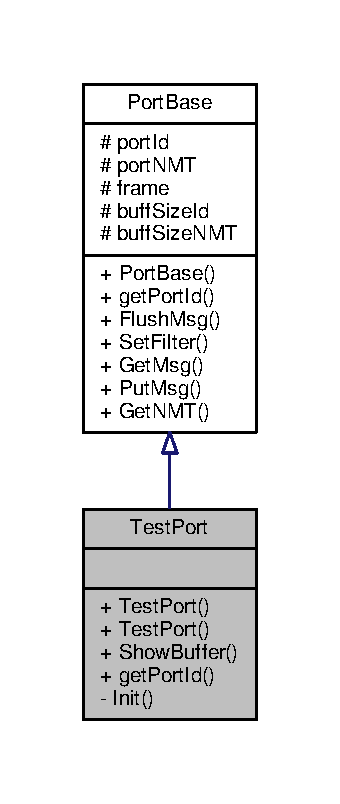
\includegraphics[width=137pt]{classTestPort__inherit__graph}
\end{center}
\end{figure}


Collaboration diagram for Test\+Port\+:
\nopagebreak
\begin{figure}[H]
\begin{center}
\leavevmode
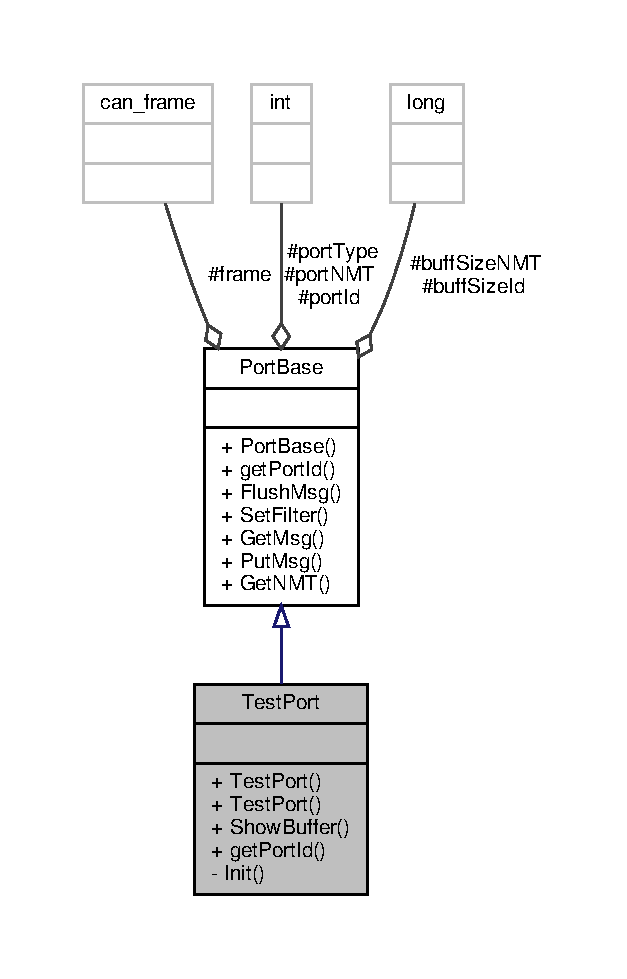
\includegraphics[width=137pt]{classTestPort__coll__graph}
\end{center}
\end{figure}
\subsection*{Public Member Functions}
\begin{DoxyCompactItemize}
\item 
\mbox{\Hypertarget{classTestPort_a93293d14818c76db0b4ef1273cf5ce19}\label{classTestPort_a93293d14818c76db0b4ef1273cf5ce19}} 
{\bfseries Test\+Port} (string Port)
\item 
\mbox{\Hypertarget{classTestPort_acc9bf1db6c1ca7d9040591306100ab36}\label{classTestPort_acc9bf1db6c1ca7d9040591306100ab36}} 
long {\bfseries Show\+Buffer} ()
\item 
\mbox{\Hypertarget{classTestPort_abf6a7327e26838aaf3e2e4482668085f}\label{classTestPort_abf6a7327e26838aaf3e2e4482668085f}} 
int {\bfseries get\+Port\+Id} ()
\end{DoxyCompactItemize}
\subsection*{Additional Inherited Members}


The documentation for this class was generated from the following files\+:\begin{DoxyCompactItemize}
\item 
Test\+Port.\+h\item 
Test\+Port.\+cpp\end{DoxyCompactItemize}

\chapter{File Documentation}
\hypertarget{CanBusPort_8cpp}{}\section{Can\+Bus\+Port.\+cpp File Reference}
\label{CanBusPort_8cpp}\index{Can\+Bus\+Port.\+cpp@{Can\+Bus\+Port.\+cpp}}
{\ttfamily \#include \char`\"{}Can\+Bus\+Port.\+h\char`\"{}}\newline
Include dependency graph for Can\+Bus\+Port.\+cpp\+:\nopagebreak
\begin{figure}[H]
\begin{center}
\leavevmode
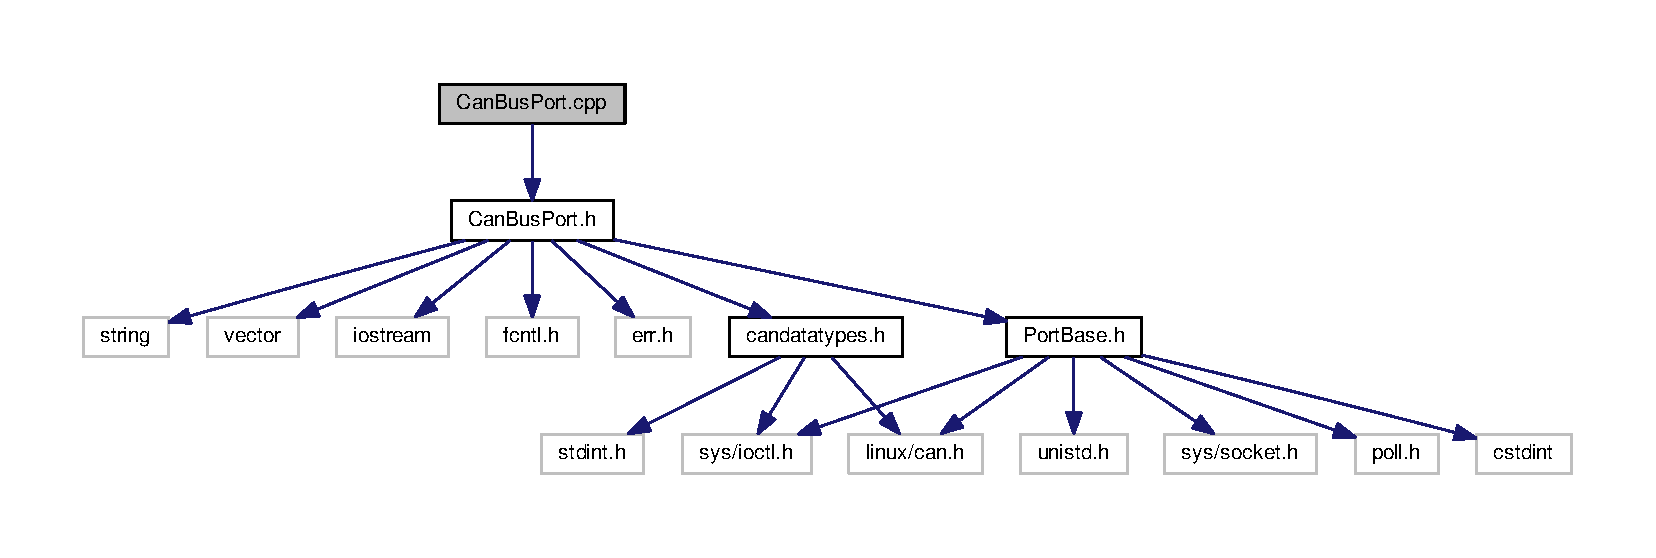
\includegraphics[width=350pt]{CanBusPort_8cpp__incl}
\end{center}
\end{figure}

\hypertarget{CanBusPort_8h}{}\section{Can\+Bus\+Port.\+h File Reference}
\label{CanBusPort_8h}\index{Can\+Bus\+Port.\+h@{Can\+Bus\+Port.\+h}}
{\ttfamily \#include $<$string$>$}\newline
{\ttfamily \#include $<$vector$>$}\newline
{\ttfamily \#include $<$iostream$>$}\newline
{\ttfamily \#include $<$fcntl.\+h$>$}\newline
{\ttfamily \#include $<$err.\+h$>$}\newline
{\ttfamily \#include \char`\"{}candatatypes.\+h\char`\"{}}\newline
{\ttfamily \#include \char`\"{}Port\+Base.\+h\char`\"{}}\newline
Include dependency graph for Can\+Bus\+Port.\+h\+:\nopagebreak
\begin{figure}[H]
\begin{center}
\leavevmode
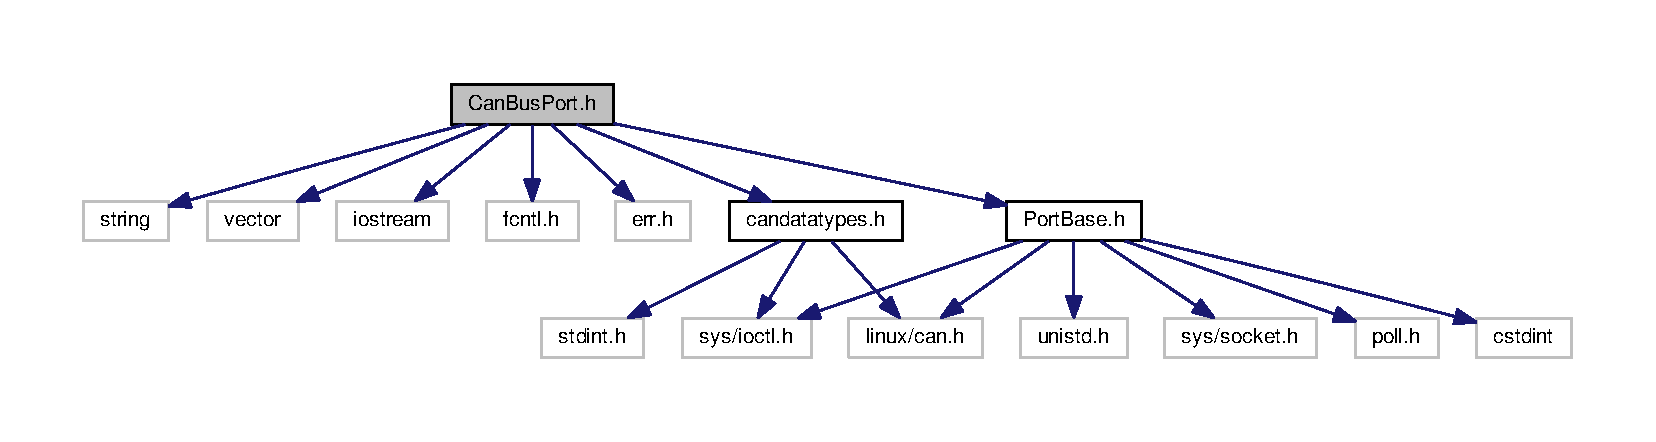
\includegraphics[width=350pt]{CanBusPort_8h__incl}
\end{center}
\end{figure}
This graph shows which files directly or indirectly include this file\+:\nopagebreak
\begin{figure}[H]
\begin{center}
\leavevmode
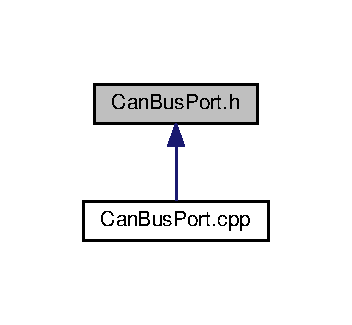
\includegraphics[width=169pt]{CanBusPort_8h__dep__incl}
\end{center}
\end{figure}
\subsection*{Classes}
\begin{DoxyCompactItemize}
\item 
class \hyperlink{classCanBusPort}{Can\+Bus\+Port}
\end{DoxyCompactItemize}

\hypertarget{candatatypes_8h}{}\section{candatatypes.\+h File Reference}
\label{candatatypes_8h}\index{candatatypes.\+h@{candatatypes.\+h}}
{\ttfamily \#include $<$linux/can.\+h$>$}\\*
{\ttfamily \#include $<$sys/ioctl.\+h$>$}\\*
{\ttfamily \#include $<$stdint.\+h$>$}\\*
Include dependency graph for candatatypes.\+h\+:
\nopagebreak
\begin{figure}[H]
\begin{center}
\leavevmode
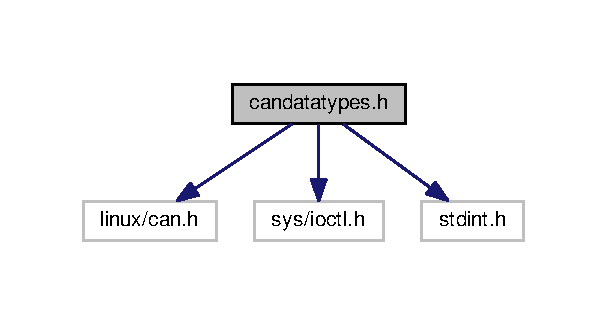
\includegraphics[width=292pt]{candatatypes_8h__incl}
\end{center}
\end{figure}
This graph shows which files directly or indirectly include this file\+:
\nopagebreak
\begin{figure}[H]
\begin{center}
\leavevmode
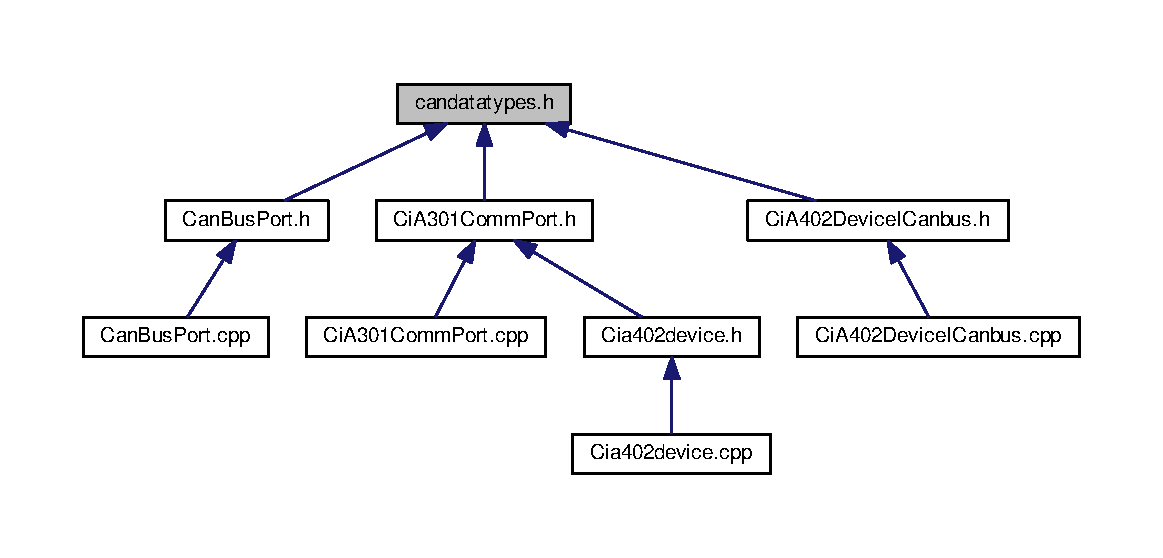
\includegraphics[width=350pt]{candatatypes_8h__dep__incl}
\end{center}
\end{figure}
\subsection*{Classes}
\begin{DoxyCompactItemize}
\item 
struct \hyperlink{structcan__msg}{can\+\_\+msg}
\item 
struct \hyperlink{structco__msg}{co\+\_\+msg}
\end{DoxyCompactItemize}
\subsection*{Macros}
\begin{DoxyCompactItemize}
\item 
\#define \hyperlink{candatatypes_8h_a37499575cbfb9909399ce3189639f122}{G\+E\+T\+\_\+\+N\+O\+D\+E\+\_\+\+ID}(cobid)~( cobid \& 0x7f )
\item 
\#define \hyperlink{candatatypes_8h_abb973a44d16fd02957aec9c47d5ac0b1}{I\+O\+C\+\_\+\+M\+A\+G\+IC}~\textquotesingle{}E\textquotesingle{}
\item 
\#define \hyperlink{candatatypes_8h_a36d525cf4d116b2fe4ecc00222b256f1}{P\+A\+C\+K\+ED}~\+\_\+\+\_\+attribute\+\_\+\+\_\+((packed))
\item 
\#define \hyperlink{candatatypes_8h_a0e6b1af48bd887e8d0c978b5dc7307bc}{M\+S\+G\+\_\+\+D\+LC}(msg)~(((msg)-\/$>$fi\&0xf)$>$$>$0)
\item 
\#define \hyperlink{candatatypes_8h_a3e5172a02bebe6e5e9706ab7df06d902}{M\+S\+G\+\_\+\+R\+TR}(msg)~(((msg)-\/$>$fi\&(1$<$$<$4))$>$$>$4)
\item 
\#define \hyperlink{candatatypes_8h_af5de903edfa22afc007f582fa19cb3d9}{M\+S\+G\+\_\+\+FF}(msg)~(((msg)-\/$>$fi\&(1$<$$<$5))$>$$>$5)
\item 
\#define \hyperlink{candatatypes_8h_a5525b28635b17a750eb630af9f82aabf}{M\+S\+G\+\_\+\+D\+OS}(msg)~(((msg)-\/$>$fi\&(1$<$$<$6))$>$$>$6)
\item 
\#define \hyperlink{candatatypes_8h_a5682e4e8de03fe4232894a36ff00b316}{M\+S\+G\+\_\+\+I\+O\+P\+IN}(msg)~(((msg)-\/$>$fi\&(1$<$$<$7))$>$$>$7)
\item 
\#define \hyperlink{candatatypes_8h_a4ad56e164b5ddbdec986135493a1fef2}{M\+S\+G\+\_\+\+N\+O\+DE}(msg)~(((msg)-\/$>$fi\&(3$<$$<$8))$>$$>$8)
\item 
\#define \hyperlink{candatatypes_8h_a04fd6b5cadb7a6b3d7b586a14545ccdb}{F\+F\+\_\+\+N\+O\+R\+M\+AL}~0
\item 
\#define \hyperlink{candatatypes_8h_a45b12438f26b30925139689e606f9231}{F\+F\+\_\+\+E\+X\+T\+E\+N\+D\+ED}~1
\item 
\#define \hyperlink{candatatypes_8h_a2e1908762e3be59ff1f1249315817f3f}{I\+O\+C\+\_\+\+R\+E\+S\+E\+T\+\_\+\+B\+O\+A\+RD}~\+\_\+\+IO (\hyperlink{hico__api_8h_abb973a44d16fd02957aec9c47d5ac0b1}{I\+O\+C\+\_\+\+M\+A\+G\+IC}, 1)
\item 
\#define \hyperlink{candatatypes_8h_a346da60de0bcf2ba4fe6d83c2439a6aa}{I\+O\+C\+\_\+\+S\+T\+A\+RT}~\+\_\+\+IO (\hyperlink{hico__api_8h_abb973a44d16fd02957aec9c47d5ac0b1}{I\+O\+C\+\_\+\+M\+A\+G\+IC}, 5)
\item 
\#define \hyperlink{candatatypes_8h_a23b340dcb801bd677be094b1db214f21}{I\+O\+C\+\_\+\+S\+T\+A\+R\+T\+\_\+\+P\+A\+S\+S\+I\+VE}~\+\_\+\+IO (\hyperlink{hico__api_8h_abb973a44d16fd02957aec9c47d5ac0b1}{I\+O\+C\+\_\+\+M\+A\+G\+IC}, 10)
\item 
\#define \hyperlink{candatatypes_8h_af8cda96f7edddada586e67abc795c9a7}{I\+O\+C\+\_\+\+S\+T\+A\+R\+T\+\_\+\+B\+A\+U\+D\+S\+C\+AN}~\+\_\+\+IO (\hyperlink{hico__api_8h_abb973a44d16fd02957aec9c47d5ac0b1}{I\+O\+C\+\_\+\+M\+A\+G\+IC}, 15)
\item 
\#define \hyperlink{candatatypes_8h_a25a17d51ed18d29864905396e2542f2a}{I\+O\+C\+\_\+\+S\+T\+OP}~\+\_\+\+IO (\hyperlink{hico__api_8h_abb973a44d16fd02957aec9c47d5ac0b1}{I\+O\+C\+\_\+\+M\+A\+G\+IC}, 20)
\item 
\#define \hyperlink{candatatypes_8h_a435f17e5332c2081e7ce09842664f183}{I\+O\+C\+\_\+\+G\+E\+T\+\_\+\+M\+O\+DE}~\+\_\+\+I\+OR(\hyperlink{hico__api_8h_abb973a44d16fd02957aec9c47d5ac0b1}{I\+O\+C\+\_\+\+M\+A\+G\+IC}, 25,  uint32\+\_\+t)
\item 
\#define \hyperlink{candatatypes_8h_aff568c17dcaa5179a247a36874b011f6}{C\+M\+\_\+\+B\+A\+U\+D\+S\+C\+AN}~1
\item 
\#define \hyperlink{candatatypes_8h_ac16bf18f66fbaf440f3dedf069a0f611}{C\+M\+\_\+\+P\+A\+S\+S\+I\+VE}~2
\item 
\#define \hyperlink{candatatypes_8h_a6c1e851b693474b1b91bb0820adfbce3}{C\+M\+\_\+\+A\+C\+T\+I\+VE}~3
\item 
\#define \hyperlink{candatatypes_8h_aa8bcd6538691e59322e8e3a03fad080a}{C\+M\+\_\+\+R\+E\+S\+ET}~4
\item 
\#define \hyperlink{candatatypes_8h_a9bcc4d1b52c43e507f264eb3d326f1c5}{I\+O\+C\+\_\+\+S\+E\+T\+\_\+\+B\+I\+T\+R\+A\+TE}~\+\_\+\+I\+OW (\hyperlink{hico__api_8h_abb973a44d16fd02957aec9c47d5ac0b1}{I\+O\+C\+\_\+\+M\+A\+G\+IC}, 30, uint32\+\_\+t)
\item 
\#define \hyperlink{candatatypes_8h_aa1ad7a89155a7f858ab52149c2fcaad5}{B\+I\+T\+R\+A\+T\+E\+\_\+10k}~0
\item 
\#define \hyperlink{candatatypes_8h_a4eb46432ed1b9dd664fc642738a1a969}{B\+I\+T\+R\+A\+T\+E\+\_\+20k}~1
\item 
\#define \hyperlink{candatatypes_8h_a39c91c0deb48d0a15d084f2a2021417b}{B\+I\+T\+R\+A\+T\+E\+\_\+50k}~2
\item 
\#define \hyperlink{candatatypes_8h_aae6f862ae12a0da0d319cd353ea7befe}{B\+I\+T\+R\+A\+T\+E\+\_\+100k}~3
\item 
\#define \hyperlink{candatatypes_8h_afbce0ed8bc362c29562f98ea81456e24}{B\+I\+T\+R\+A\+T\+E\+\_\+125k}~4
\item 
\#define \hyperlink{candatatypes_8h_a634a59a9129b549f182844e7b4058a2a}{B\+I\+T\+R\+A\+T\+E\+\_\+250k}~5
\item 
\#define \hyperlink{candatatypes_8h_a845bd49223fdabd4ebd206779eb8f3b1}{B\+I\+T\+R\+A\+T\+E\+\_\+500k}~6
\item 
\#define \hyperlink{candatatypes_8h_a8b1930fb9b23dcba55143e0ef37081fc}{B\+I\+T\+R\+A\+T\+E\+\_\+800k}~7
\item 
\#define \hyperlink{candatatypes_8h_a1432cd8532548faf2ae5287ca4a7413c}{B\+I\+T\+R\+A\+T\+E\+\_\+1000k}~8
\item 
\#define \hyperlink{candatatypes_8h_a9b5344964c96f46fcfffc44074a499a5}{I\+O\+C\+\_\+\+S\+E\+T\+\_\+\+S\+J\+W\+\_\+\+I\+N\+C\+R\+E\+M\+E\+NT}~\+\_\+\+I\+OW (\hyperlink{hico__api_8h_abb973a44d16fd02957aec9c47d5ac0b1}{I\+O\+C\+\_\+\+M\+A\+G\+IC}, 31, uint32\+\_\+t)
\item 
\#define \hyperlink{candatatypes_8h_a1be0497522ab2fd1aa5b9f7eaecda4fb}{I\+O\+C\+\_\+\+G\+E\+T\+\_\+\+B\+I\+T\+R\+A\+TE}~\+\_\+\+I\+OR (\hyperlink{hico__api_8h_abb973a44d16fd02957aec9c47d5ac0b1}{I\+O\+C\+\_\+\+M\+A\+G\+IC}, 35, uint32\+\_\+t)
\end{DoxyCompactItemize}
\subsection*{Variables}
\begin{DoxyCompactItemize}
\item 
struct \hyperlink{structcan__msg}{can\+\_\+msg} \hyperlink{candatatypes_8h_aaf243a2c10c3bb6ce08d79a9637a9a47}{P\+A\+C\+K\+ED}
\end{DoxyCompactItemize}


\subsection{Macro Definition Documentation}
\index{candatatypes.\+h@{candatatypes.\+h}!B\+I\+T\+R\+A\+T\+E\+\_\+1000k@{B\+I\+T\+R\+A\+T\+E\+\_\+1000k}}
\index{B\+I\+T\+R\+A\+T\+E\+\_\+1000k@{B\+I\+T\+R\+A\+T\+E\+\_\+1000k}!candatatypes.\+h@{candatatypes.\+h}}
\subsubsection[{\texorpdfstring{B\+I\+T\+R\+A\+T\+E\+\_\+1000k}{BITRATE_1000k}}]{\setlength{\rightskip}{0pt plus 5cm}\#define B\+I\+T\+R\+A\+T\+E\+\_\+1000k~8}\hypertarget{candatatypes_8h_a1432cd8532548faf2ae5287ca4a7413c}{}\label{candatatypes_8h_a1432cd8532548faf2ae5287ca4a7413c}
\index{candatatypes.\+h@{candatatypes.\+h}!B\+I\+T\+R\+A\+T\+E\+\_\+100k@{B\+I\+T\+R\+A\+T\+E\+\_\+100k}}
\index{B\+I\+T\+R\+A\+T\+E\+\_\+100k@{B\+I\+T\+R\+A\+T\+E\+\_\+100k}!candatatypes.\+h@{candatatypes.\+h}}
\subsubsection[{\texorpdfstring{B\+I\+T\+R\+A\+T\+E\+\_\+100k}{BITRATE_100k}}]{\setlength{\rightskip}{0pt plus 5cm}\#define B\+I\+T\+R\+A\+T\+E\+\_\+100k~3}\hypertarget{candatatypes_8h_aae6f862ae12a0da0d319cd353ea7befe}{}\label{candatatypes_8h_aae6f862ae12a0da0d319cd353ea7befe}
\index{candatatypes.\+h@{candatatypes.\+h}!B\+I\+T\+R\+A\+T\+E\+\_\+10k@{B\+I\+T\+R\+A\+T\+E\+\_\+10k}}
\index{B\+I\+T\+R\+A\+T\+E\+\_\+10k@{B\+I\+T\+R\+A\+T\+E\+\_\+10k}!candatatypes.\+h@{candatatypes.\+h}}
\subsubsection[{\texorpdfstring{B\+I\+T\+R\+A\+T\+E\+\_\+10k}{BITRATE_10k}}]{\setlength{\rightskip}{0pt plus 5cm}\#define B\+I\+T\+R\+A\+T\+E\+\_\+10k~0}\hypertarget{candatatypes_8h_aa1ad7a89155a7f858ab52149c2fcaad5}{}\label{candatatypes_8h_aa1ad7a89155a7f858ab52149c2fcaad5}
\index{candatatypes.\+h@{candatatypes.\+h}!B\+I\+T\+R\+A\+T\+E\+\_\+125k@{B\+I\+T\+R\+A\+T\+E\+\_\+125k}}
\index{B\+I\+T\+R\+A\+T\+E\+\_\+125k@{B\+I\+T\+R\+A\+T\+E\+\_\+125k}!candatatypes.\+h@{candatatypes.\+h}}
\subsubsection[{\texorpdfstring{B\+I\+T\+R\+A\+T\+E\+\_\+125k}{BITRATE_125k}}]{\setlength{\rightskip}{0pt plus 5cm}\#define B\+I\+T\+R\+A\+T\+E\+\_\+125k~4}\hypertarget{candatatypes_8h_afbce0ed8bc362c29562f98ea81456e24}{}\label{candatatypes_8h_afbce0ed8bc362c29562f98ea81456e24}
\index{candatatypes.\+h@{candatatypes.\+h}!B\+I\+T\+R\+A\+T\+E\+\_\+20k@{B\+I\+T\+R\+A\+T\+E\+\_\+20k}}
\index{B\+I\+T\+R\+A\+T\+E\+\_\+20k@{B\+I\+T\+R\+A\+T\+E\+\_\+20k}!candatatypes.\+h@{candatatypes.\+h}}
\subsubsection[{\texorpdfstring{B\+I\+T\+R\+A\+T\+E\+\_\+20k}{BITRATE_20k}}]{\setlength{\rightskip}{0pt plus 5cm}\#define B\+I\+T\+R\+A\+T\+E\+\_\+20k~1}\hypertarget{candatatypes_8h_a4eb46432ed1b9dd664fc642738a1a969}{}\label{candatatypes_8h_a4eb46432ed1b9dd664fc642738a1a969}
\index{candatatypes.\+h@{candatatypes.\+h}!B\+I\+T\+R\+A\+T\+E\+\_\+250k@{B\+I\+T\+R\+A\+T\+E\+\_\+250k}}
\index{B\+I\+T\+R\+A\+T\+E\+\_\+250k@{B\+I\+T\+R\+A\+T\+E\+\_\+250k}!candatatypes.\+h@{candatatypes.\+h}}
\subsubsection[{\texorpdfstring{B\+I\+T\+R\+A\+T\+E\+\_\+250k}{BITRATE_250k}}]{\setlength{\rightskip}{0pt plus 5cm}\#define B\+I\+T\+R\+A\+T\+E\+\_\+250k~5}\hypertarget{candatatypes_8h_a634a59a9129b549f182844e7b4058a2a}{}\label{candatatypes_8h_a634a59a9129b549f182844e7b4058a2a}
\index{candatatypes.\+h@{candatatypes.\+h}!B\+I\+T\+R\+A\+T\+E\+\_\+500k@{B\+I\+T\+R\+A\+T\+E\+\_\+500k}}
\index{B\+I\+T\+R\+A\+T\+E\+\_\+500k@{B\+I\+T\+R\+A\+T\+E\+\_\+500k}!candatatypes.\+h@{candatatypes.\+h}}
\subsubsection[{\texorpdfstring{B\+I\+T\+R\+A\+T\+E\+\_\+500k}{BITRATE_500k}}]{\setlength{\rightskip}{0pt plus 5cm}\#define B\+I\+T\+R\+A\+T\+E\+\_\+500k~6}\hypertarget{candatatypes_8h_a845bd49223fdabd4ebd206779eb8f3b1}{}\label{candatatypes_8h_a845bd49223fdabd4ebd206779eb8f3b1}
\index{candatatypes.\+h@{candatatypes.\+h}!B\+I\+T\+R\+A\+T\+E\+\_\+50k@{B\+I\+T\+R\+A\+T\+E\+\_\+50k}}
\index{B\+I\+T\+R\+A\+T\+E\+\_\+50k@{B\+I\+T\+R\+A\+T\+E\+\_\+50k}!candatatypes.\+h@{candatatypes.\+h}}
\subsubsection[{\texorpdfstring{B\+I\+T\+R\+A\+T\+E\+\_\+50k}{BITRATE_50k}}]{\setlength{\rightskip}{0pt plus 5cm}\#define B\+I\+T\+R\+A\+T\+E\+\_\+50k~2}\hypertarget{candatatypes_8h_a39c91c0deb48d0a15d084f2a2021417b}{}\label{candatatypes_8h_a39c91c0deb48d0a15d084f2a2021417b}
\index{candatatypes.\+h@{candatatypes.\+h}!B\+I\+T\+R\+A\+T\+E\+\_\+800k@{B\+I\+T\+R\+A\+T\+E\+\_\+800k}}
\index{B\+I\+T\+R\+A\+T\+E\+\_\+800k@{B\+I\+T\+R\+A\+T\+E\+\_\+800k}!candatatypes.\+h@{candatatypes.\+h}}
\subsubsection[{\texorpdfstring{B\+I\+T\+R\+A\+T\+E\+\_\+800k}{BITRATE_800k}}]{\setlength{\rightskip}{0pt plus 5cm}\#define B\+I\+T\+R\+A\+T\+E\+\_\+800k~7}\hypertarget{candatatypes_8h_a8b1930fb9b23dcba55143e0ef37081fc}{}\label{candatatypes_8h_a8b1930fb9b23dcba55143e0ef37081fc}
\index{candatatypes.\+h@{candatatypes.\+h}!C\+M\+\_\+\+A\+C\+T\+I\+VE@{C\+M\+\_\+\+A\+C\+T\+I\+VE}}
\index{C\+M\+\_\+\+A\+C\+T\+I\+VE@{C\+M\+\_\+\+A\+C\+T\+I\+VE}!candatatypes.\+h@{candatatypes.\+h}}
\subsubsection[{\texorpdfstring{C\+M\+\_\+\+A\+C\+T\+I\+VE}{CM_ACTIVE}}]{\setlength{\rightskip}{0pt plus 5cm}\#define C\+M\+\_\+\+A\+C\+T\+I\+VE~3}\hypertarget{candatatypes_8h_a6c1e851b693474b1b91bb0820adfbce3}{}\label{candatatypes_8h_a6c1e851b693474b1b91bb0820adfbce3}
\index{candatatypes.\+h@{candatatypes.\+h}!C\+M\+\_\+\+B\+A\+U\+D\+S\+C\+AN@{C\+M\+\_\+\+B\+A\+U\+D\+S\+C\+AN}}
\index{C\+M\+\_\+\+B\+A\+U\+D\+S\+C\+AN@{C\+M\+\_\+\+B\+A\+U\+D\+S\+C\+AN}!candatatypes.\+h@{candatatypes.\+h}}
\subsubsection[{\texorpdfstring{C\+M\+\_\+\+B\+A\+U\+D\+S\+C\+AN}{CM_BAUDSCAN}}]{\setlength{\rightskip}{0pt plus 5cm}\#define C\+M\+\_\+\+B\+A\+U\+D\+S\+C\+AN~1}\hypertarget{candatatypes_8h_aff568c17dcaa5179a247a36874b011f6}{}\label{candatatypes_8h_aff568c17dcaa5179a247a36874b011f6}
\index{candatatypes.\+h@{candatatypes.\+h}!C\+M\+\_\+\+P\+A\+S\+S\+I\+VE@{C\+M\+\_\+\+P\+A\+S\+S\+I\+VE}}
\index{C\+M\+\_\+\+P\+A\+S\+S\+I\+VE@{C\+M\+\_\+\+P\+A\+S\+S\+I\+VE}!candatatypes.\+h@{candatatypes.\+h}}
\subsubsection[{\texorpdfstring{C\+M\+\_\+\+P\+A\+S\+S\+I\+VE}{CM_PASSIVE}}]{\setlength{\rightskip}{0pt plus 5cm}\#define C\+M\+\_\+\+P\+A\+S\+S\+I\+VE~2}\hypertarget{candatatypes_8h_ac16bf18f66fbaf440f3dedf069a0f611}{}\label{candatatypes_8h_ac16bf18f66fbaf440f3dedf069a0f611}
\index{candatatypes.\+h@{candatatypes.\+h}!C\+M\+\_\+\+R\+E\+S\+ET@{C\+M\+\_\+\+R\+E\+S\+ET}}
\index{C\+M\+\_\+\+R\+E\+S\+ET@{C\+M\+\_\+\+R\+E\+S\+ET}!candatatypes.\+h@{candatatypes.\+h}}
\subsubsection[{\texorpdfstring{C\+M\+\_\+\+R\+E\+S\+ET}{CM_RESET}}]{\setlength{\rightskip}{0pt plus 5cm}\#define C\+M\+\_\+\+R\+E\+S\+ET~4}\hypertarget{candatatypes_8h_aa8bcd6538691e59322e8e3a03fad080a}{}\label{candatatypes_8h_aa8bcd6538691e59322e8e3a03fad080a}
\index{candatatypes.\+h@{candatatypes.\+h}!F\+F\+\_\+\+E\+X\+T\+E\+N\+D\+ED@{F\+F\+\_\+\+E\+X\+T\+E\+N\+D\+ED}}
\index{F\+F\+\_\+\+E\+X\+T\+E\+N\+D\+ED@{F\+F\+\_\+\+E\+X\+T\+E\+N\+D\+ED}!candatatypes.\+h@{candatatypes.\+h}}
\subsubsection[{\texorpdfstring{F\+F\+\_\+\+E\+X\+T\+E\+N\+D\+ED}{FF_EXTENDED}}]{\setlength{\rightskip}{0pt plus 5cm}\#define F\+F\+\_\+\+E\+X\+T\+E\+N\+D\+ED~1}\hypertarget{candatatypes_8h_a45b12438f26b30925139689e606f9231}{}\label{candatatypes_8h_a45b12438f26b30925139689e606f9231}
\index{candatatypes.\+h@{candatatypes.\+h}!F\+F\+\_\+\+N\+O\+R\+M\+AL@{F\+F\+\_\+\+N\+O\+R\+M\+AL}}
\index{F\+F\+\_\+\+N\+O\+R\+M\+AL@{F\+F\+\_\+\+N\+O\+R\+M\+AL}!candatatypes.\+h@{candatatypes.\+h}}
\subsubsection[{\texorpdfstring{F\+F\+\_\+\+N\+O\+R\+M\+AL}{FF_NORMAL}}]{\setlength{\rightskip}{0pt plus 5cm}\#define F\+F\+\_\+\+N\+O\+R\+M\+AL~0}\hypertarget{candatatypes_8h_a04fd6b5cadb7a6b3d7b586a14545ccdb}{}\label{candatatypes_8h_a04fd6b5cadb7a6b3d7b586a14545ccdb}
\index{candatatypes.\+h@{candatatypes.\+h}!G\+E\+T\+\_\+\+N\+O\+D\+E\+\_\+\+ID@{G\+E\+T\+\_\+\+N\+O\+D\+E\+\_\+\+ID}}
\index{G\+E\+T\+\_\+\+N\+O\+D\+E\+\_\+\+ID@{G\+E\+T\+\_\+\+N\+O\+D\+E\+\_\+\+ID}!candatatypes.\+h@{candatatypes.\+h}}
\subsubsection[{\texorpdfstring{G\+E\+T\+\_\+\+N\+O\+D\+E\+\_\+\+ID}{GET_NODE_ID}}]{\setlength{\rightskip}{0pt plus 5cm}\#define G\+E\+T\+\_\+\+N\+O\+D\+E\+\_\+\+ID(
\begin{DoxyParamCaption}
\item[{}]{cobid}
\end{DoxyParamCaption}
)~( cobid \& 0x7f )}\hypertarget{candatatypes_8h_a37499575cbfb9909399ce3189639f122}{}\label{candatatypes_8h_a37499575cbfb9909399ce3189639f122}
\index{candatatypes.\+h@{candatatypes.\+h}!I\+O\+C\+\_\+\+G\+E\+T\+\_\+\+B\+I\+T\+R\+A\+TE@{I\+O\+C\+\_\+\+G\+E\+T\+\_\+\+B\+I\+T\+R\+A\+TE}}
\index{I\+O\+C\+\_\+\+G\+E\+T\+\_\+\+B\+I\+T\+R\+A\+TE@{I\+O\+C\+\_\+\+G\+E\+T\+\_\+\+B\+I\+T\+R\+A\+TE}!candatatypes.\+h@{candatatypes.\+h}}
\subsubsection[{\texorpdfstring{I\+O\+C\+\_\+\+G\+E\+T\+\_\+\+B\+I\+T\+R\+A\+TE}{IOC_GET_BITRATE}}]{\setlength{\rightskip}{0pt plus 5cm}\#define I\+O\+C\+\_\+\+G\+E\+T\+\_\+\+B\+I\+T\+R\+A\+TE~\+\_\+\+I\+OR ({\bf I\+O\+C\+\_\+\+M\+A\+G\+IC}, 35, uint32\+\_\+t)}\hypertarget{candatatypes_8h_a1be0497522ab2fd1aa5b9f7eaecda4fb}{}\label{candatatypes_8h_a1be0497522ab2fd1aa5b9f7eaecda4fb}
\index{candatatypes.\+h@{candatatypes.\+h}!I\+O\+C\+\_\+\+G\+E\+T\+\_\+\+M\+O\+DE@{I\+O\+C\+\_\+\+G\+E\+T\+\_\+\+M\+O\+DE}}
\index{I\+O\+C\+\_\+\+G\+E\+T\+\_\+\+M\+O\+DE@{I\+O\+C\+\_\+\+G\+E\+T\+\_\+\+M\+O\+DE}!candatatypes.\+h@{candatatypes.\+h}}
\subsubsection[{\texorpdfstring{I\+O\+C\+\_\+\+G\+E\+T\+\_\+\+M\+O\+DE}{IOC_GET_MODE}}]{\setlength{\rightskip}{0pt plus 5cm}\#define I\+O\+C\+\_\+\+G\+E\+T\+\_\+\+M\+O\+DE~\+\_\+\+I\+OR({\bf I\+O\+C\+\_\+\+M\+A\+G\+IC}, 25,  uint32\+\_\+t)}\hypertarget{candatatypes_8h_a435f17e5332c2081e7ce09842664f183}{}\label{candatatypes_8h_a435f17e5332c2081e7ce09842664f183}
\index{candatatypes.\+h@{candatatypes.\+h}!I\+O\+C\+\_\+\+M\+A\+G\+IC@{I\+O\+C\+\_\+\+M\+A\+G\+IC}}
\index{I\+O\+C\+\_\+\+M\+A\+G\+IC@{I\+O\+C\+\_\+\+M\+A\+G\+IC}!candatatypes.\+h@{candatatypes.\+h}}
\subsubsection[{\texorpdfstring{I\+O\+C\+\_\+\+M\+A\+G\+IC}{IOC_MAGIC}}]{\setlength{\rightskip}{0pt plus 5cm}\#define I\+O\+C\+\_\+\+M\+A\+G\+IC~\textquotesingle{}E\textquotesingle{}}\hypertarget{candatatypes_8h_abb973a44d16fd02957aec9c47d5ac0b1}{}\label{candatatypes_8h_abb973a44d16fd02957aec9c47d5ac0b1}
\index{candatatypes.\+h@{candatatypes.\+h}!I\+O\+C\+\_\+\+R\+E\+S\+E\+T\+\_\+\+B\+O\+A\+RD@{I\+O\+C\+\_\+\+R\+E\+S\+E\+T\+\_\+\+B\+O\+A\+RD}}
\index{I\+O\+C\+\_\+\+R\+E\+S\+E\+T\+\_\+\+B\+O\+A\+RD@{I\+O\+C\+\_\+\+R\+E\+S\+E\+T\+\_\+\+B\+O\+A\+RD}!candatatypes.\+h@{candatatypes.\+h}}
\subsubsection[{\texorpdfstring{I\+O\+C\+\_\+\+R\+E\+S\+E\+T\+\_\+\+B\+O\+A\+RD}{IOC_RESET_BOARD}}]{\setlength{\rightskip}{0pt plus 5cm}\#define I\+O\+C\+\_\+\+R\+E\+S\+E\+T\+\_\+\+B\+O\+A\+RD~\+\_\+\+IO ({\bf I\+O\+C\+\_\+\+M\+A\+G\+IC}, 1)}\hypertarget{candatatypes_8h_a2e1908762e3be59ff1f1249315817f3f}{}\label{candatatypes_8h_a2e1908762e3be59ff1f1249315817f3f}
\index{candatatypes.\+h@{candatatypes.\+h}!I\+O\+C\+\_\+\+S\+E\+T\+\_\+\+B\+I\+T\+R\+A\+TE@{I\+O\+C\+\_\+\+S\+E\+T\+\_\+\+B\+I\+T\+R\+A\+TE}}
\index{I\+O\+C\+\_\+\+S\+E\+T\+\_\+\+B\+I\+T\+R\+A\+TE@{I\+O\+C\+\_\+\+S\+E\+T\+\_\+\+B\+I\+T\+R\+A\+TE}!candatatypes.\+h@{candatatypes.\+h}}
\subsubsection[{\texorpdfstring{I\+O\+C\+\_\+\+S\+E\+T\+\_\+\+B\+I\+T\+R\+A\+TE}{IOC_SET_BITRATE}}]{\setlength{\rightskip}{0pt plus 5cm}\#define I\+O\+C\+\_\+\+S\+E\+T\+\_\+\+B\+I\+T\+R\+A\+TE~\+\_\+\+I\+OW ({\bf I\+O\+C\+\_\+\+M\+A\+G\+IC}, 30, uint32\+\_\+t)}\hypertarget{candatatypes_8h_a9bcc4d1b52c43e507f264eb3d326f1c5}{}\label{candatatypes_8h_a9bcc4d1b52c43e507f264eb3d326f1c5}
\index{candatatypes.\+h@{candatatypes.\+h}!I\+O\+C\+\_\+\+S\+E\+T\+\_\+\+S\+J\+W\+\_\+\+I\+N\+C\+R\+E\+M\+E\+NT@{I\+O\+C\+\_\+\+S\+E\+T\+\_\+\+S\+J\+W\+\_\+\+I\+N\+C\+R\+E\+M\+E\+NT}}
\index{I\+O\+C\+\_\+\+S\+E\+T\+\_\+\+S\+J\+W\+\_\+\+I\+N\+C\+R\+E\+M\+E\+NT@{I\+O\+C\+\_\+\+S\+E\+T\+\_\+\+S\+J\+W\+\_\+\+I\+N\+C\+R\+E\+M\+E\+NT}!candatatypes.\+h@{candatatypes.\+h}}
\subsubsection[{\texorpdfstring{I\+O\+C\+\_\+\+S\+E\+T\+\_\+\+S\+J\+W\+\_\+\+I\+N\+C\+R\+E\+M\+E\+NT}{IOC_SET_SJW_INCREMENT}}]{\setlength{\rightskip}{0pt plus 5cm}\#define I\+O\+C\+\_\+\+S\+E\+T\+\_\+\+S\+J\+W\+\_\+\+I\+N\+C\+R\+E\+M\+E\+NT~\+\_\+\+I\+OW ({\bf I\+O\+C\+\_\+\+M\+A\+G\+IC}, 31, uint32\+\_\+t)}\hypertarget{candatatypes_8h_a9b5344964c96f46fcfffc44074a499a5}{}\label{candatatypes_8h_a9b5344964c96f46fcfffc44074a499a5}
\index{candatatypes.\+h@{candatatypes.\+h}!I\+O\+C\+\_\+\+S\+T\+A\+RT@{I\+O\+C\+\_\+\+S\+T\+A\+RT}}
\index{I\+O\+C\+\_\+\+S\+T\+A\+RT@{I\+O\+C\+\_\+\+S\+T\+A\+RT}!candatatypes.\+h@{candatatypes.\+h}}
\subsubsection[{\texorpdfstring{I\+O\+C\+\_\+\+S\+T\+A\+RT}{IOC_START}}]{\setlength{\rightskip}{0pt plus 5cm}\#define I\+O\+C\+\_\+\+S\+T\+A\+RT~\+\_\+\+IO ({\bf I\+O\+C\+\_\+\+M\+A\+G\+IC}, 5)}\hypertarget{candatatypes_8h_a346da60de0bcf2ba4fe6d83c2439a6aa}{}\label{candatatypes_8h_a346da60de0bcf2ba4fe6d83c2439a6aa}
\index{candatatypes.\+h@{candatatypes.\+h}!I\+O\+C\+\_\+\+S\+T\+A\+R\+T\+\_\+\+B\+A\+U\+D\+S\+C\+AN@{I\+O\+C\+\_\+\+S\+T\+A\+R\+T\+\_\+\+B\+A\+U\+D\+S\+C\+AN}}
\index{I\+O\+C\+\_\+\+S\+T\+A\+R\+T\+\_\+\+B\+A\+U\+D\+S\+C\+AN@{I\+O\+C\+\_\+\+S\+T\+A\+R\+T\+\_\+\+B\+A\+U\+D\+S\+C\+AN}!candatatypes.\+h@{candatatypes.\+h}}
\subsubsection[{\texorpdfstring{I\+O\+C\+\_\+\+S\+T\+A\+R\+T\+\_\+\+B\+A\+U\+D\+S\+C\+AN}{IOC_START_BAUDSCAN}}]{\setlength{\rightskip}{0pt plus 5cm}\#define I\+O\+C\+\_\+\+S\+T\+A\+R\+T\+\_\+\+B\+A\+U\+D\+S\+C\+AN~\+\_\+\+IO ({\bf I\+O\+C\+\_\+\+M\+A\+G\+IC}, 15)}\hypertarget{candatatypes_8h_af8cda96f7edddada586e67abc795c9a7}{}\label{candatatypes_8h_af8cda96f7edddada586e67abc795c9a7}
\index{candatatypes.\+h@{candatatypes.\+h}!I\+O\+C\+\_\+\+S\+T\+A\+R\+T\+\_\+\+P\+A\+S\+S\+I\+VE@{I\+O\+C\+\_\+\+S\+T\+A\+R\+T\+\_\+\+P\+A\+S\+S\+I\+VE}}
\index{I\+O\+C\+\_\+\+S\+T\+A\+R\+T\+\_\+\+P\+A\+S\+S\+I\+VE@{I\+O\+C\+\_\+\+S\+T\+A\+R\+T\+\_\+\+P\+A\+S\+S\+I\+VE}!candatatypes.\+h@{candatatypes.\+h}}
\subsubsection[{\texorpdfstring{I\+O\+C\+\_\+\+S\+T\+A\+R\+T\+\_\+\+P\+A\+S\+S\+I\+VE}{IOC_START_PASSIVE}}]{\setlength{\rightskip}{0pt plus 5cm}\#define I\+O\+C\+\_\+\+S\+T\+A\+R\+T\+\_\+\+P\+A\+S\+S\+I\+VE~\+\_\+\+IO ({\bf I\+O\+C\+\_\+\+M\+A\+G\+IC}, 10)}\hypertarget{candatatypes_8h_a23b340dcb801bd677be094b1db214f21}{}\label{candatatypes_8h_a23b340dcb801bd677be094b1db214f21}
\index{candatatypes.\+h@{candatatypes.\+h}!I\+O\+C\+\_\+\+S\+T\+OP@{I\+O\+C\+\_\+\+S\+T\+OP}}
\index{I\+O\+C\+\_\+\+S\+T\+OP@{I\+O\+C\+\_\+\+S\+T\+OP}!candatatypes.\+h@{candatatypes.\+h}}
\subsubsection[{\texorpdfstring{I\+O\+C\+\_\+\+S\+T\+OP}{IOC_STOP}}]{\setlength{\rightskip}{0pt plus 5cm}\#define I\+O\+C\+\_\+\+S\+T\+OP~\+\_\+\+IO ({\bf I\+O\+C\+\_\+\+M\+A\+G\+IC}, 20)}\hypertarget{candatatypes_8h_a25a17d51ed18d29864905396e2542f2a}{}\label{candatatypes_8h_a25a17d51ed18d29864905396e2542f2a}
\index{candatatypes.\+h@{candatatypes.\+h}!M\+S\+G\+\_\+\+D\+LC@{M\+S\+G\+\_\+\+D\+LC}}
\index{M\+S\+G\+\_\+\+D\+LC@{M\+S\+G\+\_\+\+D\+LC}!candatatypes.\+h@{candatatypes.\+h}}
\subsubsection[{\texorpdfstring{M\+S\+G\+\_\+\+D\+LC}{MSG_DLC}}]{\setlength{\rightskip}{0pt plus 5cm}\#define M\+S\+G\+\_\+\+D\+LC(
\begin{DoxyParamCaption}
\item[{}]{msg}
\end{DoxyParamCaption}
)~(((msg)-\/$>$fi\&0xf)$>$$>$0)}\hypertarget{candatatypes_8h_a0e6b1af48bd887e8d0c978b5dc7307bc}{}\label{candatatypes_8h_a0e6b1af48bd887e8d0c978b5dc7307bc}
\index{candatatypes.\+h@{candatatypes.\+h}!M\+S\+G\+\_\+\+D\+OS@{M\+S\+G\+\_\+\+D\+OS}}
\index{M\+S\+G\+\_\+\+D\+OS@{M\+S\+G\+\_\+\+D\+OS}!candatatypes.\+h@{candatatypes.\+h}}
\subsubsection[{\texorpdfstring{M\+S\+G\+\_\+\+D\+OS}{MSG_DOS}}]{\setlength{\rightskip}{0pt plus 5cm}\#define M\+S\+G\+\_\+\+D\+OS(
\begin{DoxyParamCaption}
\item[{}]{msg}
\end{DoxyParamCaption}
)~(((msg)-\/$>$fi\&(1$<$$<$6))$>$$>$6)}\hypertarget{candatatypes_8h_a5525b28635b17a750eb630af9f82aabf}{}\label{candatatypes_8h_a5525b28635b17a750eb630af9f82aabf}
\index{candatatypes.\+h@{candatatypes.\+h}!M\+S\+G\+\_\+\+FF@{M\+S\+G\+\_\+\+FF}}
\index{M\+S\+G\+\_\+\+FF@{M\+S\+G\+\_\+\+FF}!candatatypes.\+h@{candatatypes.\+h}}
\subsubsection[{\texorpdfstring{M\+S\+G\+\_\+\+FF}{MSG_FF}}]{\setlength{\rightskip}{0pt plus 5cm}\#define M\+S\+G\+\_\+\+FF(
\begin{DoxyParamCaption}
\item[{}]{msg}
\end{DoxyParamCaption}
)~(((msg)-\/$>$fi\&(1$<$$<$5))$>$$>$5)}\hypertarget{candatatypes_8h_af5de903edfa22afc007f582fa19cb3d9}{}\label{candatatypes_8h_af5de903edfa22afc007f582fa19cb3d9}
\index{candatatypes.\+h@{candatatypes.\+h}!M\+S\+G\+\_\+\+I\+O\+P\+IN@{M\+S\+G\+\_\+\+I\+O\+P\+IN}}
\index{M\+S\+G\+\_\+\+I\+O\+P\+IN@{M\+S\+G\+\_\+\+I\+O\+P\+IN}!candatatypes.\+h@{candatatypes.\+h}}
\subsubsection[{\texorpdfstring{M\+S\+G\+\_\+\+I\+O\+P\+IN}{MSG_IOPIN}}]{\setlength{\rightskip}{0pt plus 5cm}\#define M\+S\+G\+\_\+\+I\+O\+P\+IN(
\begin{DoxyParamCaption}
\item[{}]{msg}
\end{DoxyParamCaption}
)~(((msg)-\/$>$fi\&(1$<$$<$7))$>$$>$7)}\hypertarget{candatatypes_8h_a5682e4e8de03fe4232894a36ff00b316}{}\label{candatatypes_8h_a5682e4e8de03fe4232894a36ff00b316}
\index{candatatypes.\+h@{candatatypes.\+h}!M\+S\+G\+\_\+\+N\+O\+DE@{M\+S\+G\+\_\+\+N\+O\+DE}}
\index{M\+S\+G\+\_\+\+N\+O\+DE@{M\+S\+G\+\_\+\+N\+O\+DE}!candatatypes.\+h@{candatatypes.\+h}}
\subsubsection[{\texorpdfstring{M\+S\+G\+\_\+\+N\+O\+DE}{MSG_NODE}}]{\setlength{\rightskip}{0pt plus 5cm}\#define M\+S\+G\+\_\+\+N\+O\+DE(
\begin{DoxyParamCaption}
\item[{}]{msg}
\end{DoxyParamCaption}
)~(((msg)-\/$>$fi\&(3$<$$<$8))$>$$>$8)}\hypertarget{candatatypes_8h_a4ad56e164b5ddbdec986135493a1fef2}{}\label{candatatypes_8h_a4ad56e164b5ddbdec986135493a1fef2}
\index{candatatypes.\+h@{candatatypes.\+h}!M\+S\+G\+\_\+\+R\+TR@{M\+S\+G\+\_\+\+R\+TR}}
\index{M\+S\+G\+\_\+\+R\+TR@{M\+S\+G\+\_\+\+R\+TR}!candatatypes.\+h@{candatatypes.\+h}}
\subsubsection[{\texorpdfstring{M\+S\+G\+\_\+\+R\+TR}{MSG_RTR}}]{\setlength{\rightskip}{0pt plus 5cm}\#define M\+S\+G\+\_\+\+R\+TR(
\begin{DoxyParamCaption}
\item[{}]{msg}
\end{DoxyParamCaption}
)~(((msg)-\/$>$fi\&(1$<$$<$4))$>$$>$4)}\hypertarget{candatatypes_8h_a3e5172a02bebe6e5e9706ab7df06d902}{}\label{candatatypes_8h_a3e5172a02bebe6e5e9706ab7df06d902}
\index{candatatypes.\+h@{candatatypes.\+h}!P\+A\+C\+K\+ED@{P\+A\+C\+K\+ED}}
\index{P\+A\+C\+K\+ED@{P\+A\+C\+K\+ED}!candatatypes.\+h@{candatatypes.\+h}}
\subsubsection[{\texorpdfstring{P\+A\+C\+K\+ED}{PACKED}}]{\setlength{\rightskip}{0pt plus 5cm}\#define P\+A\+C\+K\+ED~\+\_\+\+\_\+attribute\+\_\+\+\_\+((packed))}\hypertarget{candatatypes_8h_a36d525cf4d116b2fe4ecc00222b256f1}{}\label{candatatypes_8h_a36d525cf4d116b2fe4ecc00222b256f1}


\subsection{Variable Documentation}
\index{candatatypes.\+h@{candatatypes.\+h}!P\+A\+C\+K\+ED@{P\+A\+C\+K\+ED}}
\index{P\+A\+C\+K\+ED@{P\+A\+C\+K\+ED}!candatatypes.\+h@{candatatypes.\+h}}
\subsubsection[{\texorpdfstring{P\+A\+C\+K\+ED}{PACKED}}]{\setlength{\rightskip}{0pt plus 5cm}struct {\bf can\+\_\+msg} P\+A\+C\+K\+ED}\hypertarget{candatatypes_8h_aaf243a2c10c3bb6ce08d79a9637a9a47}{}\label{candatatypes_8h_aaf243a2c10c3bb6ce08d79a9637a9a47}

\hypertarget{CiA301CommPort_8cpp}{}\section{Ci\+A301\+Comm\+Port.\+cpp File Reference}
\label{CiA301CommPort_8cpp}\index{Ci\+A301\+Comm\+Port.\+cpp@{Ci\+A301\+Comm\+Port.\+cpp}}
{\ttfamily \#include \char`\"{}Ci\+A301\+Comm\+Port.\+h\char`\"{}}\newline
Include dependency graph for Ci\+A301\+Comm\+Port.\+cpp\+:\nopagebreak
\begin{figure}[H]
\begin{center}
\leavevmode
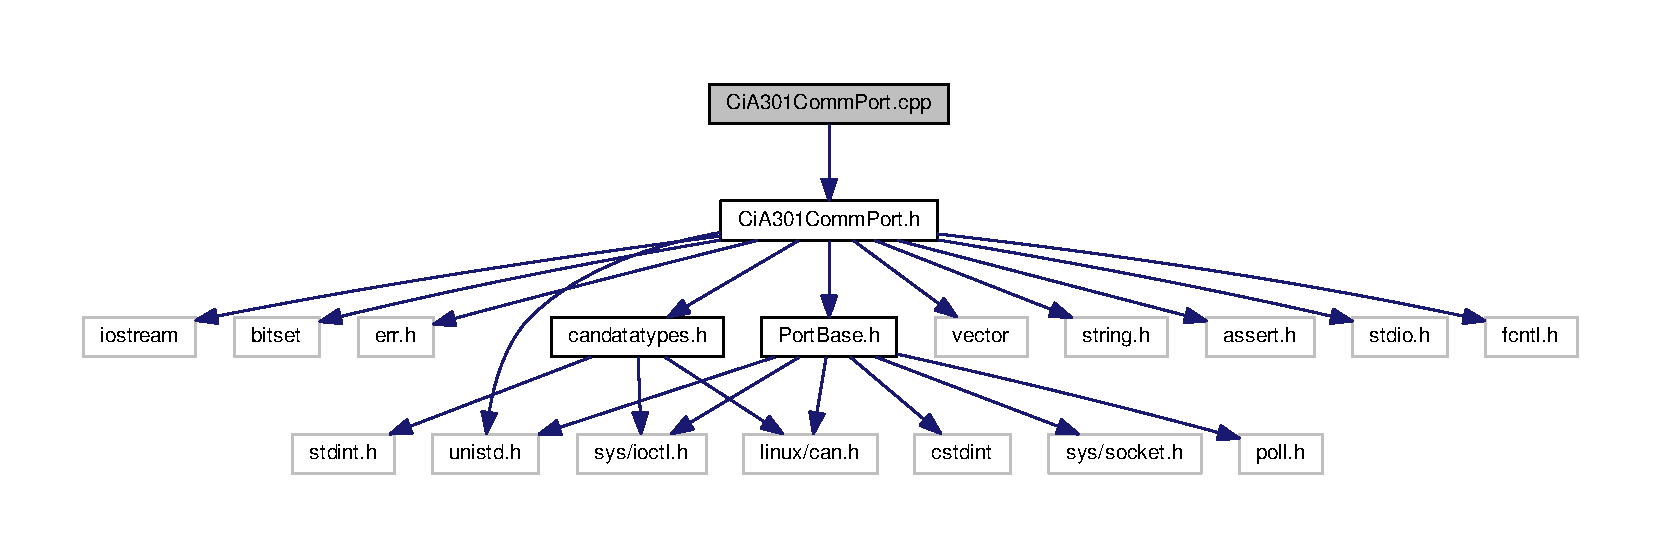
\includegraphics[width=350pt]{CiA301CommPort_8cpp__incl}
\end{center}
\end{figure}

\hypertarget{CiA301CommPort_8h}{}\section{Ci\+A301\+Comm\+Port.\+h File Reference}
\label{CiA301CommPort_8h}\index{Ci\+A301\+Comm\+Port.\+h@{Ci\+A301\+Comm\+Port.\+h}}
{\ttfamily \#include $<$iostream$>$}\newline
{\ttfamily \#include $<$bitset$>$}\newline
{\ttfamily \#include $<$err.\+h$>$}\newline
{\ttfamily \#include $<$unistd.\+h$>$}\newline
{\ttfamily \#include $<$vector$>$}\newline
{\ttfamily \#include $<$string.\+h$>$}\newline
{\ttfamily \#include $<$assert.\+h$>$}\newline
{\ttfamily \#include $<$stdio.\+h$>$}\newline
{\ttfamily \#include $<$fcntl.\+h$>$}\newline
{\ttfamily \#include \char`\"{}candatatypes.\+h\char`\"{}}\newline
{\ttfamily \#include \char`\"{}Port\+Base.\+h\char`\"{}}\newline
Include dependency graph for Ci\+A301\+Comm\+Port.\+h\+:\nopagebreak
\begin{figure}[H]
\begin{center}
\leavevmode
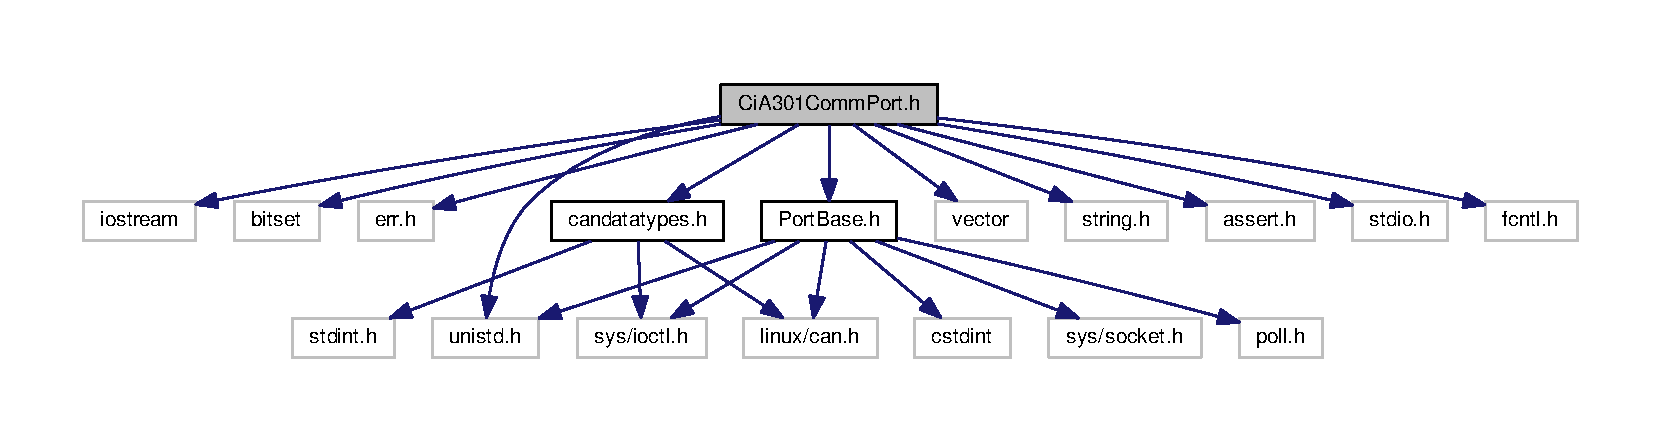
\includegraphics[width=350pt]{CiA301CommPort_8h__incl}
\end{center}
\end{figure}
This graph shows which files directly or indirectly include this file\+:
\nopagebreak
\begin{figure}[H]
\begin{center}
\leavevmode
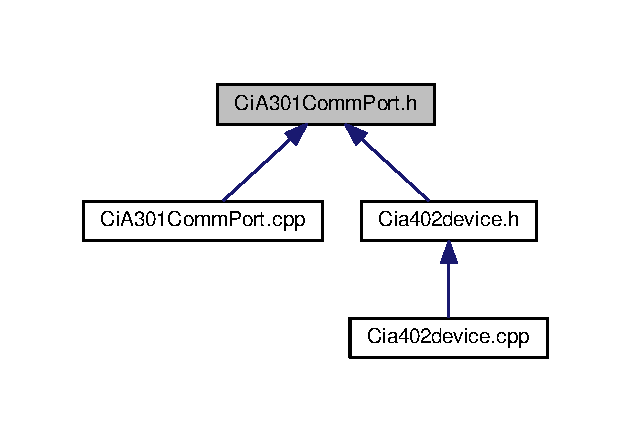
\includegraphics[width=350pt]{CiA301CommPort_8h__dep__incl}
\end{center}
\end{figure}
\subsection*{Classes}
\begin{DoxyCompactItemize}
\item 
class \hyperlink{classCiA301CommPort}{Ci\+A301\+Comm\+Port}
\end{DoxyCompactItemize}
\subsection*{Namespaces}
\begin{DoxyCompactItemize}
\item 
 \hyperlink{namespacesdo}{sdo}
\item 
 \hyperlink{namespacepdo}{pdo}
\item 
 \hyperlink{namespacenmt}{nmt}
\end{DoxyCompactItemize}
\subsection*{Macros}
\begin{DoxyCompactItemize}
\item 
\#define \hyperlink{CiA301CommPort_8h_a9c4538b32717c71448f328bccbf80784}{U\+S\+E\+\_\+\+T\+I\+M\+E\+O\+UT}~200
\item 
\#define \hyperlink{CiA301CommPort_8h_a1ac42c9168b067855b5bb1e8e96afb62}{F\+I\+N\+D\+\_\+\+R\+E\+T\+RY}~20
\end{DoxyCompactItemize}
\subsection*{Variables}
\begin{DoxyCompactItemize}
\item 
const uint16\+\_\+t \hyperlink{namespacesdo_ada4eb9ed2535da14a1b4c449b52c98b6}{sdo\+::tx0} =0x580
\item 
const uint16\+\_\+t \hyperlink{namespacesdo_a32e87699bc0a4deed591fb38703c48f2}{sdo\+::rx0} =0x600
\item 
const uint16\+\_\+t \hyperlink{namespacepdo_a4a8e678f87bbe2520c5cffe3f6a6dae0}{pdo\+::tx0} =0x180
\item 
const uint16\+\_\+t \hyperlink{namespacepdo_a3a8ecb285207c4eb0b05bc69762404cf}{pdo\+::rx0} =0x200
\item 
const uint16\+\_\+t \hyperlink{namespacepdo_ae5f87d5007685cfd9d219e1cb051ccf0}{pdo\+::tx1} =0x280
\item 
const uint16\+\_\+t \hyperlink{namespacepdo_a1388fefc691ccce0ef2ea8347f737d1d}{pdo\+::rx1} =0x300
\item 
const uint16\+\_\+t \hyperlink{namespacepdo_a12b62b143e83e83b2566dea6d20a169a}{pdo\+::tx4} =0x380
\item 
const uint16\+\_\+t \hyperlink{namespacepdo_ab45e1d027abca75c1d406d514d3f6085}{pdo\+::rx4} =0x400
\item 
const vector$<$ uint8\+\_\+t $>$ \hyperlink{namespacenmt_a1310e5c59553352490180a42ef1dad8c}{nmt\+::started} =\{0x01\}
\end{DoxyCompactItemize}


\subsection{Macro Definition Documentation}
\mbox{\Hypertarget{CiA301CommPort_8h_a1ac42c9168b067855b5bb1e8e96afb62}\label{CiA301CommPort_8h_a1ac42c9168b067855b5bb1e8e96afb62}} 
\index{Ci\+A301\+Comm\+Port.\+h@{Ci\+A301\+Comm\+Port.\+h}!F\+I\+N\+D\+\_\+\+R\+E\+T\+RY@{F\+I\+N\+D\+\_\+\+R\+E\+T\+RY}}
\index{F\+I\+N\+D\+\_\+\+R\+E\+T\+RY@{F\+I\+N\+D\+\_\+\+R\+E\+T\+RY}!Ci\+A301\+Comm\+Port.\+h@{Ci\+A301\+Comm\+Port.\+h}}
\subsubsection{\texorpdfstring{F\+I\+N\+D\+\_\+\+R\+E\+T\+RY}{FIND\_RETRY}}
{\footnotesize\ttfamily \#define F\+I\+N\+D\+\_\+\+R\+E\+T\+RY~20}

\mbox{\Hypertarget{CiA301CommPort_8h_a9c4538b32717c71448f328bccbf80784}\label{CiA301CommPort_8h_a9c4538b32717c71448f328bccbf80784}} 
\index{Ci\+A301\+Comm\+Port.\+h@{Ci\+A301\+Comm\+Port.\+h}!U\+S\+E\+\_\+\+T\+I\+M\+E\+O\+UT@{U\+S\+E\+\_\+\+T\+I\+M\+E\+O\+UT}}
\index{U\+S\+E\+\_\+\+T\+I\+M\+E\+O\+UT@{U\+S\+E\+\_\+\+T\+I\+M\+E\+O\+UT}!Ci\+A301\+Comm\+Port.\+h@{Ci\+A301\+Comm\+Port.\+h}}
\subsubsection{\texorpdfstring{U\+S\+E\+\_\+\+T\+I\+M\+E\+O\+UT}{USE\_TIMEOUT}}
{\footnotesize\ttfamily \#define U\+S\+E\+\_\+\+T\+I\+M\+E\+O\+UT~200}


\hypertarget{Cia402device_8cpp}{}\section{Cia402device.\+cpp File Reference}
\label{Cia402device_8cpp}\index{Cia402device.\+cpp@{Cia402device.\+cpp}}
{\ttfamily \#include \char`\"{}Cia402device.\+h\char`\"{}}\newline
Include dependency graph for Cia402device.\+cpp\+:
\nopagebreak
\begin{figure}[H]
\begin{center}
\leavevmode
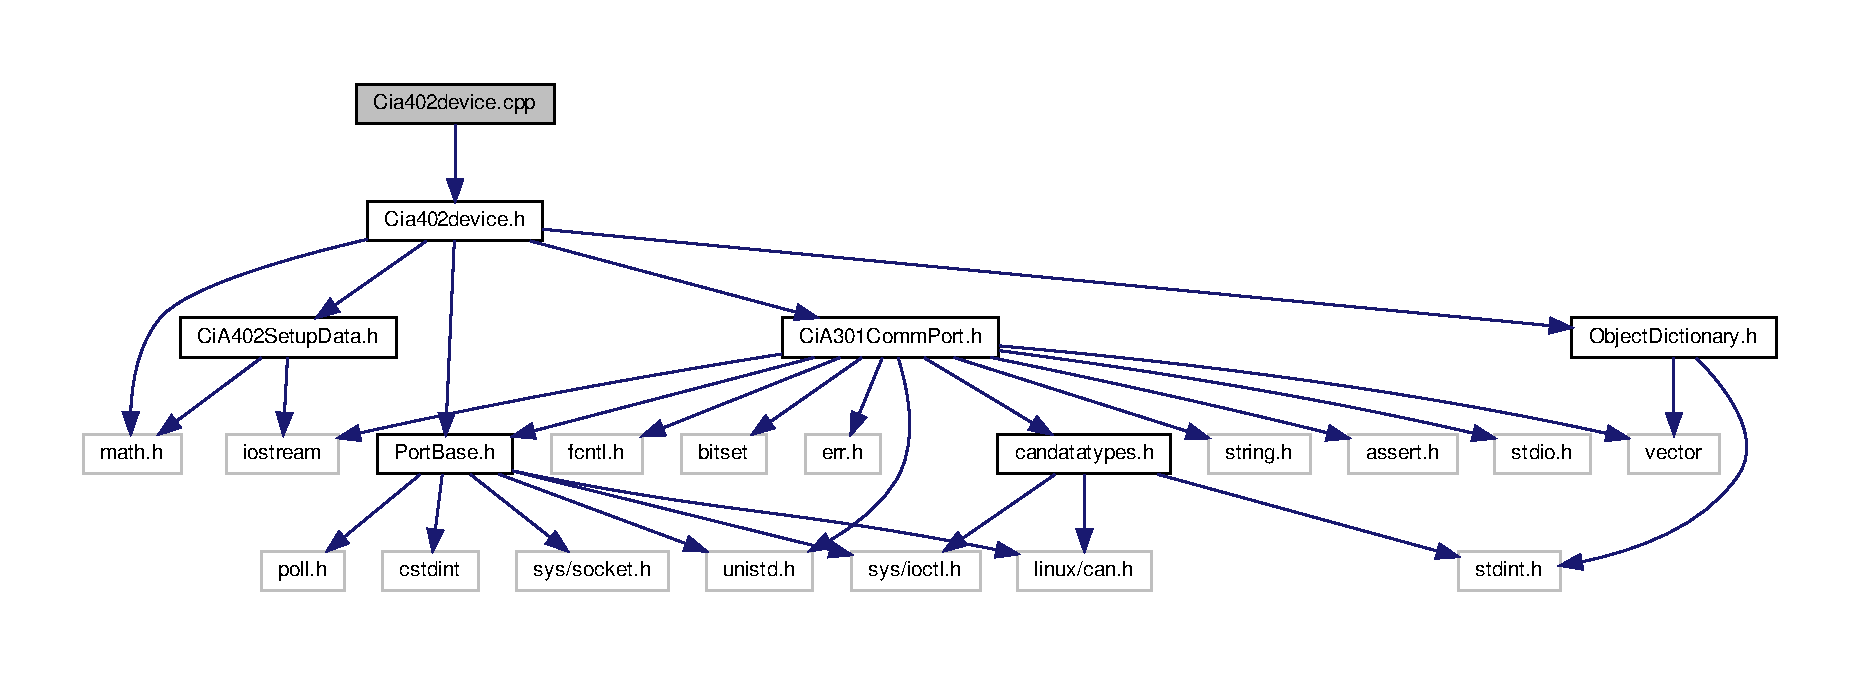
\includegraphics[width=350pt]{Cia402device_8cpp__incl}
\end{center}
\end{figure}
\subsection*{Functions}
\begin{DoxyCompactItemize}
\item 
vector$<$ uint8\+\_\+t $>$ \hyperlink{Cia402device_8cpp_ae234205c3014b4a69b38fff2c9602132}{data32to4x8} (uint32\+\_\+t in)
\item 
vector$<$ uint8\+\_\+t $>$ \hyperlink{Cia402device_8cpp_ab66ff1d3349b2b4fb19ffe21e8b1269a}{data16to2x8} (uint16\+\_\+t in)
\end{DoxyCompactItemize}


\subsection{Function Documentation}
\mbox{\Hypertarget{Cia402device_8cpp_ab66ff1d3349b2b4fb19ffe21e8b1269a}\label{Cia402device_8cpp_ab66ff1d3349b2b4fb19ffe21e8b1269a}} 
\index{Cia402device.\+cpp@{Cia402device.\+cpp}!data16to2x8@{data16to2x8}}
\index{data16to2x8@{data16to2x8}!Cia402device.\+cpp@{Cia402device.\+cpp}}
\subsubsection{\texorpdfstring{data16to2x8()}{data16to2x8()}}
{\footnotesize\ttfamily vector$<$ uint8\+\_\+t $>$ data16to2x8 (\begin{DoxyParamCaption}\item[{uint16\+\_\+t}]{in }\end{DoxyParamCaption})}

\mbox{\Hypertarget{Cia402device_8cpp_ae234205c3014b4a69b38fff2c9602132}\label{Cia402device_8cpp_ae234205c3014b4a69b38fff2c9602132}} 
\index{Cia402device.\+cpp@{Cia402device.\+cpp}!data32to4x8@{data32to4x8}}
\index{data32to4x8@{data32to4x8}!Cia402device.\+cpp@{Cia402device.\+cpp}}
\subsubsection{\texorpdfstring{data32to4x8()}{data32to4x8()}}
{\footnotesize\ttfamily vector$<$ uint8\+\_\+t $>$ data32to4x8 (\begin{DoxyParamCaption}\item[{uint32\+\_\+t}]{in }\end{DoxyParamCaption})}


\hypertarget{Cia402device_8h}{}\section{Cia402device.\+h File Reference}
\label{Cia402device_8h}\index{Cia402device.\+h@{Cia402device.\+h}}
{\ttfamily \#include $<$math.\+h$>$}\newline
{\ttfamily \#include \char`\"{}Ci\+A301\+Comm\+Port.\+h\char`\"{}}\newline
{\ttfamily \#include \char`\"{}Object\+Dictionary.\+h\char`\"{}}\newline
{\ttfamily \#include \char`\"{}Port\+Base.\+h\char`\"{}}\newline
Include dependency graph for Cia402device.\+h\+:
\nopagebreak
\begin{figure}[H]
\begin{center}
\leavevmode
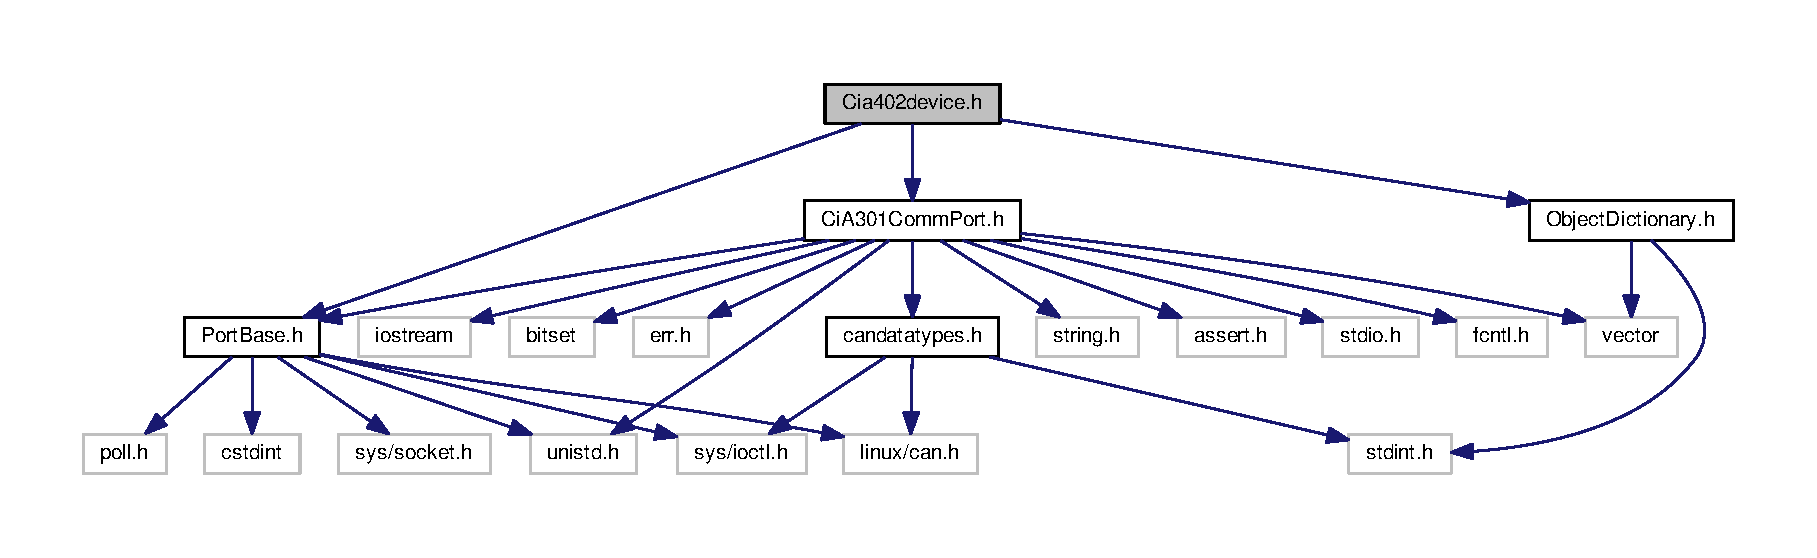
\includegraphics[width=350pt]{Cia402device_8h__incl}
\end{center}
\end{figure}
This graph shows which files directly or indirectly include this file\+:
\nopagebreak
\begin{figure}[H]
\begin{center}
\leavevmode
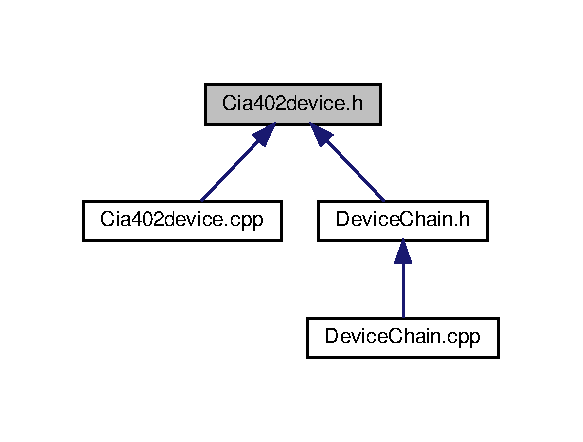
\includegraphics[width=280pt]{Cia402device_8h__dep__incl}
\end{center}
\end{figure}
\subsection*{Classes}
\begin{DoxyCompactItemize}
\item 
class \hyperlink{classCiA402Device}{Ci\+A402\+Device}
\end{DoxyCompactItemize}

\hypertarget{CiA402DeviceICanbus_8cpp}{}\section{Ci\+A402\+Device\+I\+Canbus.\+cpp File Reference}
\label{CiA402DeviceICanbus_8cpp}\index{Ci\+A402\+Device\+I\+Canbus.\+cpp@{Ci\+A402\+Device\+I\+Canbus.\+cpp}}
{\ttfamily \#include \char`\"{}Ci\+A402\+Device\+I\+Canbus.\+h\char`\"{}}\\*
Include dependency graph for Ci\+A402\+Device\+I\+Canbus.\+cpp\+:
\nopagebreak
\begin{figure}[H]
\begin{center}
\leavevmode
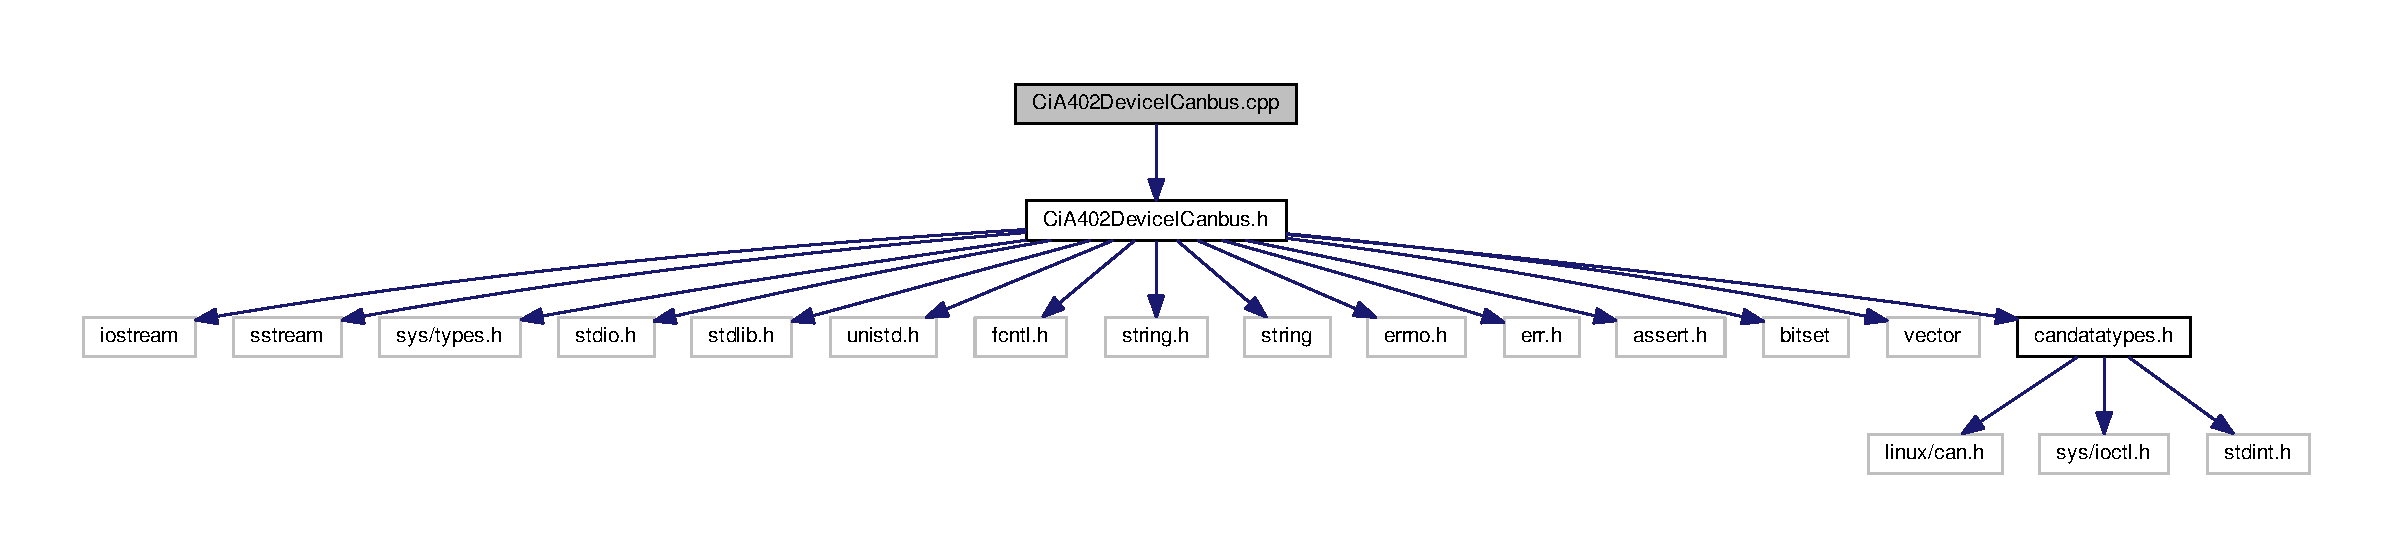
\includegraphics[width=350pt]{CiA402DeviceICanbus_8cpp__incl}
\end{center}
\end{figure}
\subsection*{Macros}
\begin{DoxyCompactItemize}
\item 
\#define \hyperlink{CiA402DeviceICanbus_8cpp_a9c4538b32717c71448f328bccbf80784}{U\+S\+E\+\_\+\+T\+I\+M\+E\+O\+UT}~200
\end{DoxyCompactItemize}


\subsection{Macro Definition Documentation}
\index{Ci\+A402\+Device\+I\+Canbus.\+cpp@{Ci\+A402\+Device\+I\+Canbus.\+cpp}!U\+S\+E\+\_\+\+T\+I\+M\+E\+O\+UT@{U\+S\+E\+\_\+\+T\+I\+M\+E\+O\+UT}}
\index{U\+S\+E\+\_\+\+T\+I\+M\+E\+O\+UT@{U\+S\+E\+\_\+\+T\+I\+M\+E\+O\+UT}!Ci\+A402\+Device\+I\+Canbus.\+cpp@{Ci\+A402\+Device\+I\+Canbus.\+cpp}}
\subsubsection[{\texorpdfstring{U\+S\+E\+\_\+\+T\+I\+M\+E\+O\+UT}{USE_TIMEOUT}}]{\setlength{\rightskip}{0pt plus 5cm}\#define U\+S\+E\+\_\+\+T\+I\+M\+E\+O\+UT~200}\hypertarget{CiA402DeviceICanbus_8cpp_a9c4538b32717c71448f328bccbf80784}{}\label{CiA402DeviceICanbus_8cpp_a9c4538b32717c71448f328bccbf80784}

\hypertarget{CiA402DeviceICanbus_8h}{}\section{Ci\+A402\+Device\+I\+Canbus.\+h File Reference}
\label{CiA402DeviceICanbus_8h}\index{Ci\+A402\+Device\+I\+Canbus.\+h@{Ci\+A402\+Device\+I\+Canbus.\+h}}
{\ttfamily \#include $<$iostream$>$}\newline
{\ttfamily \#include $<$sstream$>$}\newline
{\ttfamily \#include $<$sys/types.\+h$>$}\newline
{\ttfamily \#include $<$stdio.\+h$>$}\newline
{\ttfamily \#include $<$stdlib.\+h$>$}\newline
{\ttfamily \#include $<$unistd.\+h$>$}\newline
{\ttfamily \#include $<$fcntl.\+h$>$}\newline
{\ttfamily \#include $<$string.\+h$>$}\newline
{\ttfamily \#include $<$string$>$}\newline
{\ttfamily \#include $<$errno.\+h$>$}\newline
{\ttfamily \#include $<$err.\+h$>$}\newline
{\ttfamily \#include $<$assert.\+h$>$}\newline
{\ttfamily \#include $<$bitset$>$}\newline
{\ttfamily \#include $<$vector$>$}\newline
{\ttfamily \#include \char`\"{}candatatypes.\+h\char`\"{}}\newline
Include dependency graph for Ci\+A402\+Device\+I\+Canbus.\+h\+:\nopagebreak
\begin{figure}[H]
\begin{center}
\leavevmode
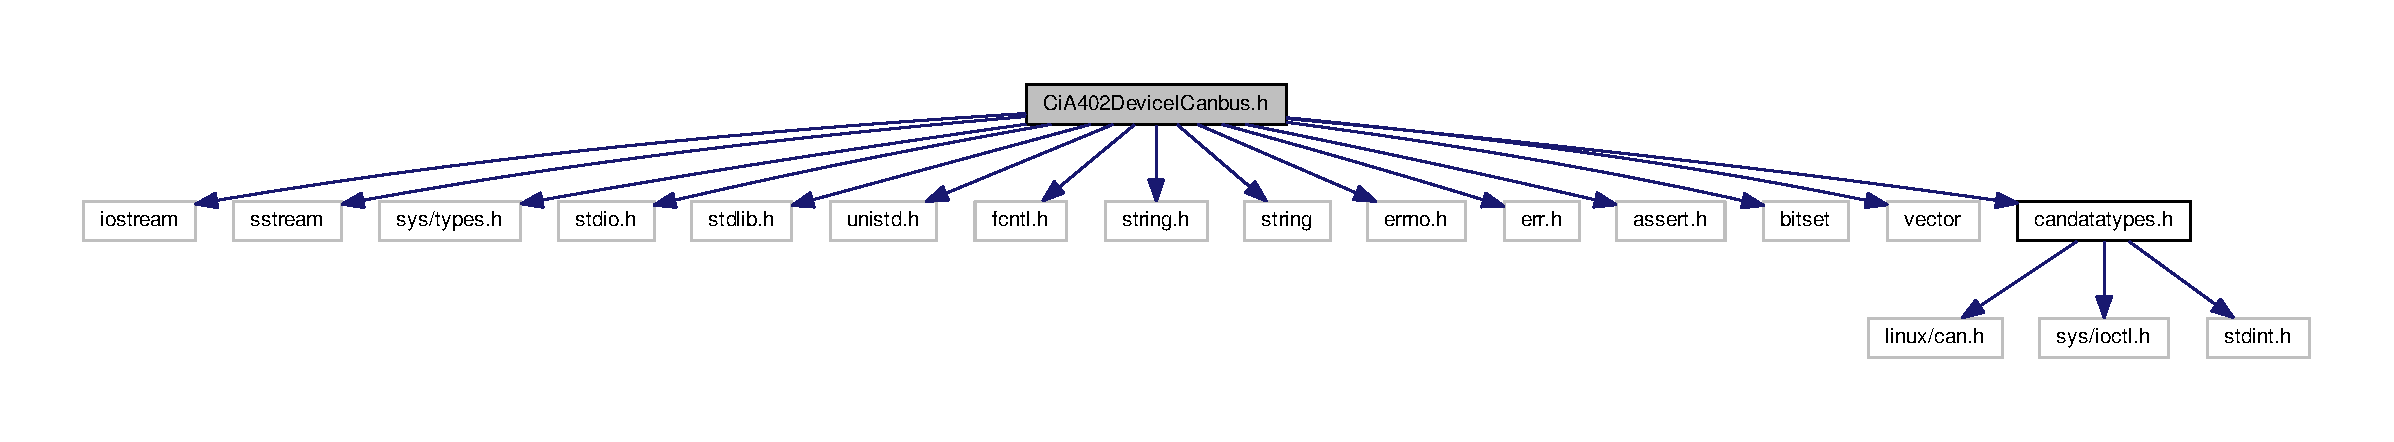
\includegraphics[width=350pt]{CiA402DeviceICanbus_8h__incl}
\end{center}
\end{figure}
This graph shows which files directly or indirectly include this file\+:\nopagebreak
\begin{figure}[H]
\begin{center}
\leavevmode
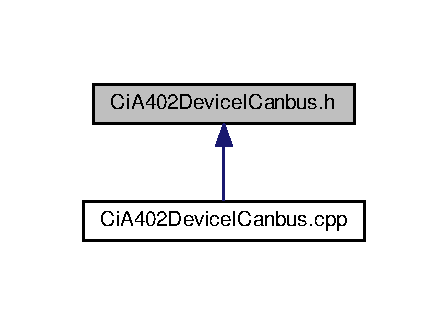
\includegraphics[width=215pt]{CiA402DeviceICanbus_8h__dep__incl}
\end{center}
\end{figure}
\subsection*{Classes}
\begin{DoxyCompactItemize}
\item 
class \hyperlink{classCiA402DeviceICanbus}{Ci\+A402\+Device\+I\+Canbus}
\end{DoxyCompactItemize}

\hypertarget{CiA402SetupData_8cpp}{}\section{Ci\+A402\+Setup\+Data.\+cpp File Reference}
\label{CiA402SetupData_8cpp}\index{Ci\+A402\+Setup\+Data.\+cpp@{Ci\+A402\+Setup\+Data.\+cpp}}
{\ttfamily \#include \char`\"{}Ci\+A402\+Setup\+Data.\+h\char`\"{}}\\*
Include dependency graph for Ci\+A402\+Setup\+Data.\+cpp\+:
\nopagebreak
\begin{figure}[H]
\begin{center}
\leavevmode
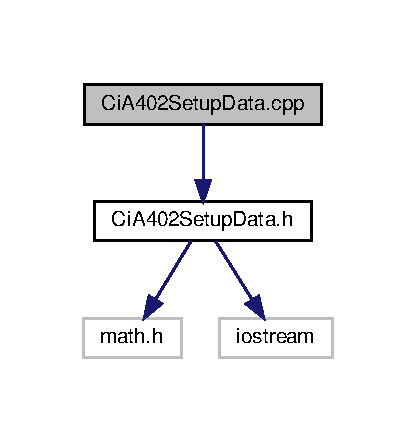
\includegraphics[width=200pt]{CiA402SetupData_8cpp__incl}
\end{center}
\end{figure}

\hypertarget{CiA402SetupData_8h}{}\section{Ci\+A402\+Setup\+Data.\+h File Reference}
\label{CiA402SetupData_8h}\index{Ci\+A402\+Setup\+Data.\+h@{Ci\+A402\+Setup\+Data.\+h}}
{\ttfamily \#include $<$math.\+h$>$}\newline
{\ttfamily \#include $<$iostream$>$}\newline
Include dependency graph for Ci\+A402\+Setup\+Data.\+h\+:
\nopagebreak
\begin{figure}[H]
\begin{center}
\leavevmode
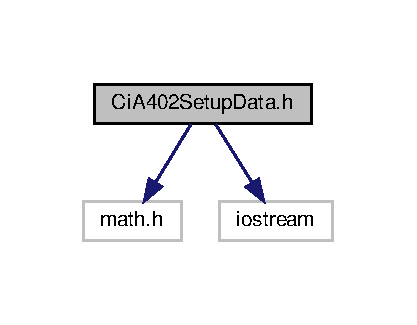
\includegraphics[width=200pt]{CiA402SetupData_8h__incl}
\end{center}
\end{figure}
This graph shows which files directly or indirectly include this file\+:
\nopagebreak
\begin{figure}[H]
\begin{center}
\leavevmode
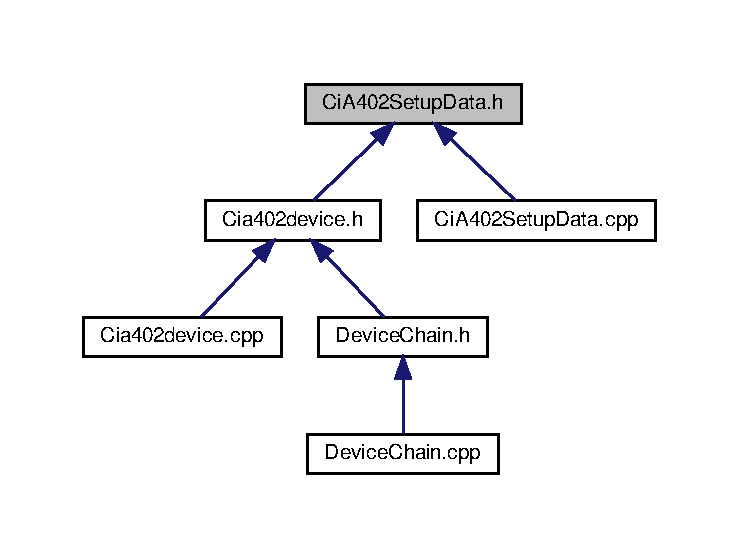
\includegraphics[width=350pt]{CiA402SetupData_8h__dep__incl}
\end{center}
\end{figure}
\subsection*{Classes}
\begin{DoxyCompactItemize}
\item 
class \hyperlink{classCiA402SetupData}{Ci\+A402\+Setup\+Data}
\end{DoxyCompactItemize}

\hypertarget{co__msg_8h}{}\section{co\+\_\+msg.\+h File Reference}
\label{co__msg_8h}\index{co\+\_\+msg.\+h@{co\+\_\+msg.\+h}}
\subsection*{Classes}
\begin{DoxyCompactItemize}
\item 
struct \hyperlink{structco__msg}{co\+\_\+msg}
\end{DoxyCompactItemize}

\hypertarget{DeviceChain_8cpp}{}\section{Device\+Chain.\+cpp File Reference}
\label{DeviceChain_8cpp}\index{Device\+Chain.\+cpp@{Device\+Chain.\+cpp}}
{\ttfamily \#include \char`\"{}Device\+Chain.\+h\char`\"{}}\newline
Include dependency graph for Device\+Chain.\+cpp\+:
\nopagebreak
\begin{figure}[H]
\begin{center}
\leavevmode
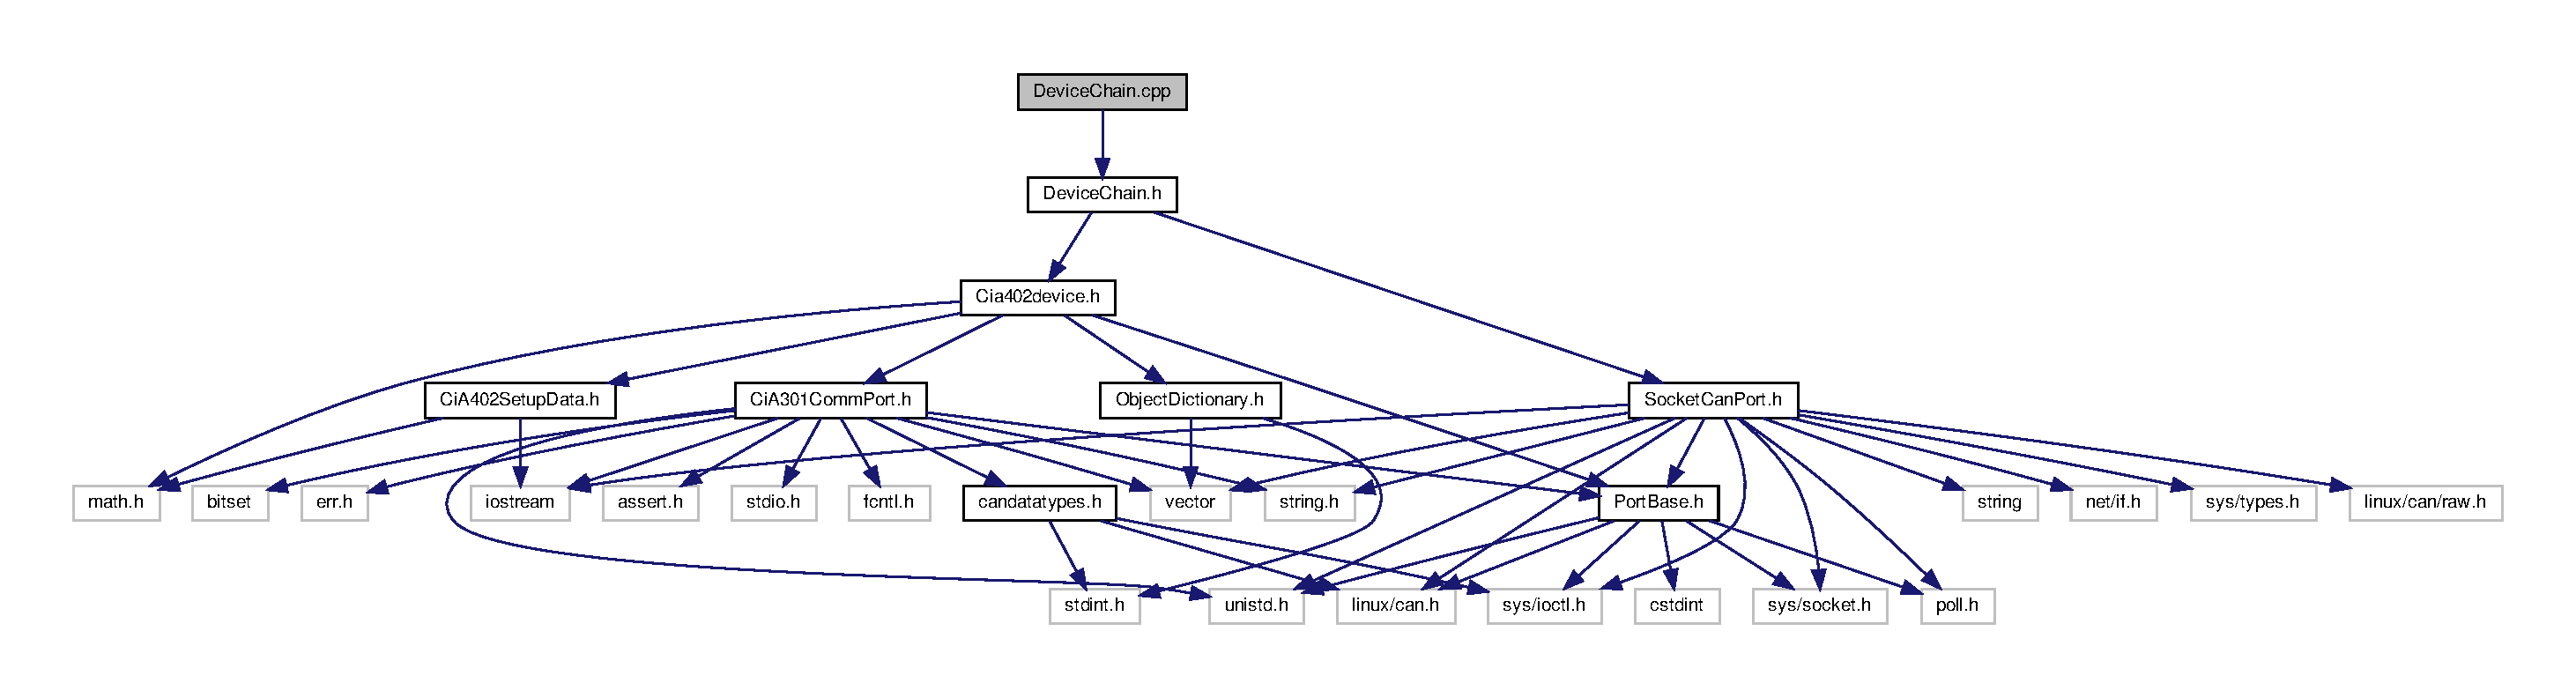
\includegraphics[width=350pt]{DeviceChain_8cpp__incl}
\end{center}
\end{figure}

\hypertarget{DeviceChain_8h}{}\section{Device\+Chain.\+h File Reference}
\label{DeviceChain_8h}\index{Device\+Chain.\+h@{Device\+Chain.\+h}}
{\ttfamily \#include \char`\"{}Cia402device.\+h\char`\"{}}\newline
{\ttfamily \#include \char`\"{}Socket\+Can\+Port.\+h\char`\"{}}\newline
Include dependency graph for Device\+Chain.\+h\+:\nopagebreak
\begin{figure}[H]
\begin{center}
\leavevmode
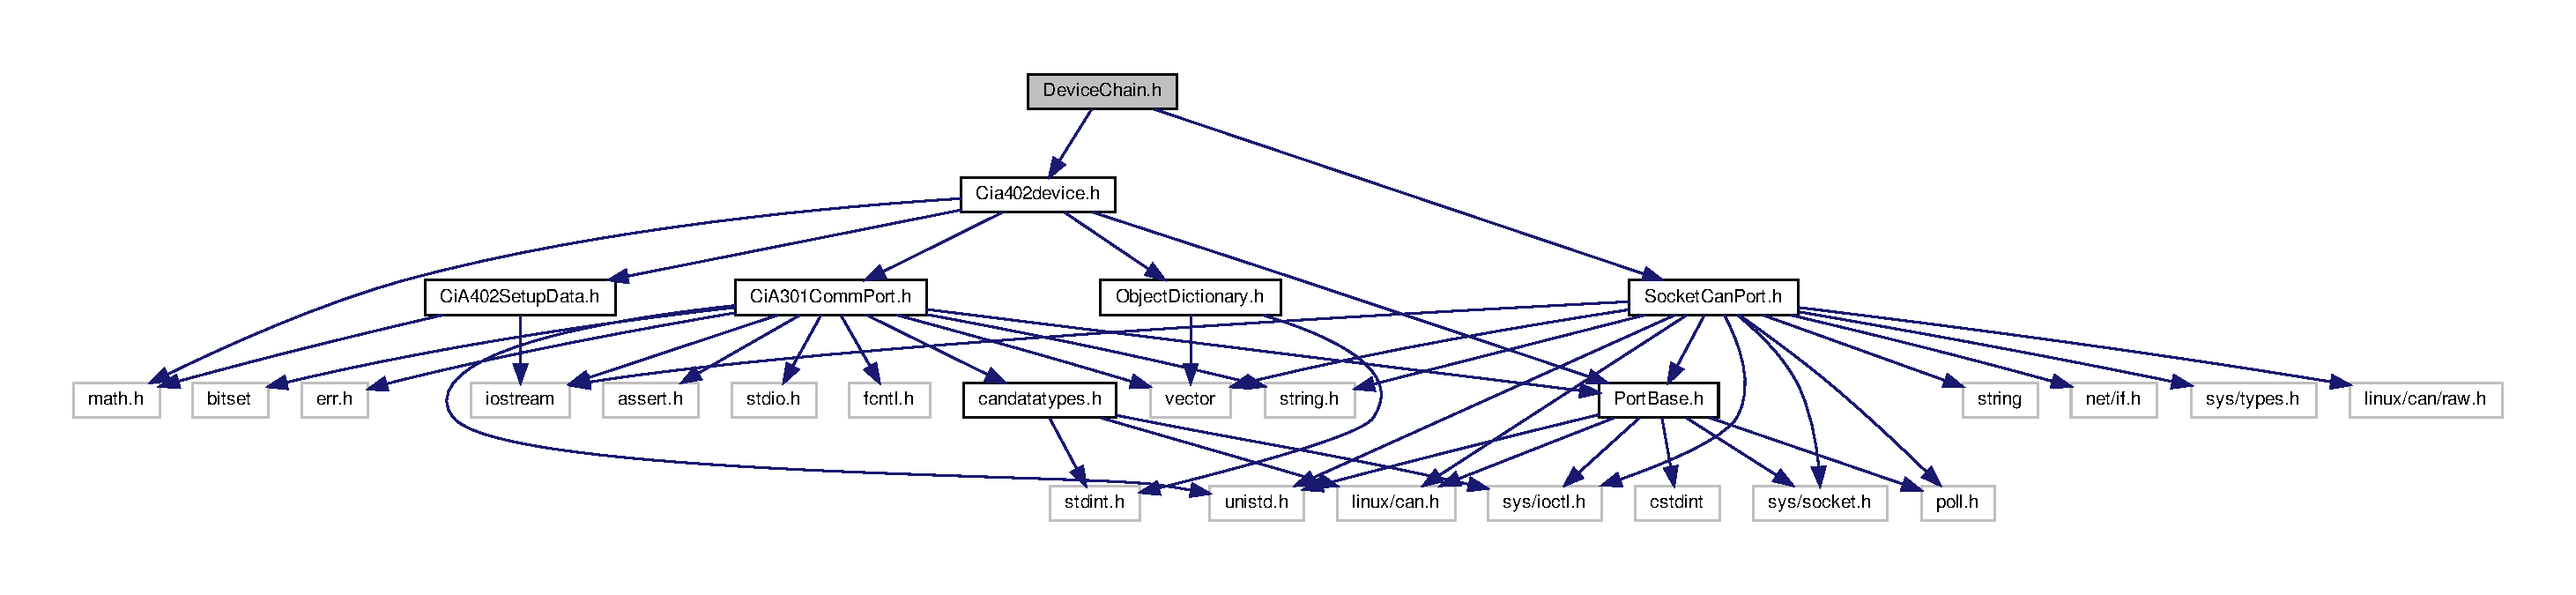
\includegraphics[width=350pt]{DeviceChain_8h__incl}
\end{center}
\end{figure}
This graph shows which files directly or indirectly include this file\+:\nopagebreak
\begin{figure}[H]
\begin{center}
\leavevmode
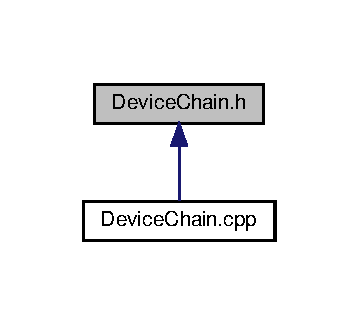
\includegraphics[width=172pt]{DeviceChain_8h__dep__incl}
\end{center}
\end{figure}
\subsection*{Classes}
\begin{DoxyCompactItemize}
\item 
class \hyperlink{classDeviceChain}{Device\+Chain}
\end{DoxyCompactItemize}

\hypertarget{hico__api_8h}{}\section{hico\+\_\+api.\+h File Reference}
\label{hico__api_8h}\index{hico\+\_\+api.\+h@{hico\+\_\+api.\+h}}
{\ttfamily \#include $<$sys/ioctl.\+h$>$}\newline
{\ttfamily \#include $<$stdint.\+h$>$}\newline
Include dependency graph for hico\+\_\+api.\+h\+:\nopagebreak
\begin{figure}[H]
\begin{center}
\leavevmode
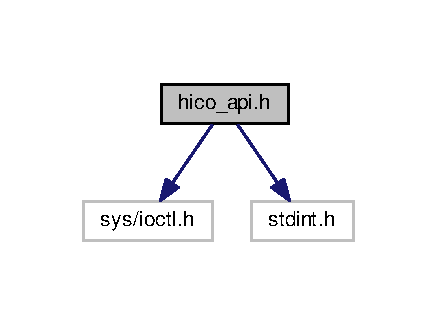
\includegraphics[width=210pt]{hico__api_8h__incl}
\end{center}
\end{figure}
\subsection*{Classes}
\begin{DoxyCompactItemize}
\item 
struct \hyperlink{structerr__stat}{err\+\_\+stat}
\item 
struct \hyperlink{structcan__msg}{can\+\_\+msg}
\item 
struct \hyperlink{structcan__filter}{can\+\_\+filter}
\end{DoxyCompactItemize}
\subsection*{Macros}
\begin{DoxyCompactItemize}
\item 
\#define \hyperlink{hico__api_8h_abb973a44d16fd02957aec9c47d5ac0b1}{I\+O\+C\+\_\+\+M\+A\+G\+IC}~\textquotesingle{}E\textquotesingle{}
\item 
\#define \hyperlink{hico__api_8h_a36d525cf4d116b2fe4ecc00222b256f1}{P\+A\+C\+K\+ED}~\+\_\+\+\_\+attribute\+\_\+\+\_\+((packed))
\item 
\#define \hyperlink{hico__api_8h_a2e1908762e3be59ff1f1249315817f3f}{I\+O\+C\+\_\+\+R\+E\+S\+E\+T\+\_\+\+B\+O\+A\+RD}~\+\_\+\+IO (\hyperlink{hico__api_8h_abb973a44d16fd02957aec9c47d5ac0b1}{I\+O\+C\+\_\+\+M\+A\+G\+IC}, 1)
\item 
\#define \hyperlink{hico__api_8h_a346da60de0bcf2ba4fe6d83c2439a6aa}{I\+O\+C\+\_\+\+S\+T\+A\+RT}~\+\_\+\+IO (\hyperlink{hico__api_8h_abb973a44d16fd02957aec9c47d5ac0b1}{I\+O\+C\+\_\+\+M\+A\+G\+IC}, 5)
\item 
\#define \hyperlink{hico__api_8h_a23b340dcb801bd677be094b1db214f21}{I\+O\+C\+\_\+\+S\+T\+A\+R\+T\+\_\+\+P\+A\+S\+S\+I\+VE}~\+\_\+\+IO (\hyperlink{hico__api_8h_abb973a44d16fd02957aec9c47d5ac0b1}{I\+O\+C\+\_\+\+M\+A\+G\+IC}, 10)
\item 
\#define \hyperlink{hico__api_8h_af8cda96f7edddada586e67abc795c9a7}{I\+O\+C\+\_\+\+S\+T\+A\+R\+T\+\_\+\+B\+A\+U\+D\+S\+C\+AN}~\+\_\+\+IO (\hyperlink{hico__api_8h_abb973a44d16fd02957aec9c47d5ac0b1}{I\+O\+C\+\_\+\+M\+A\+G\+IC}, 15)
\item 
\#define \hyperlink{hico__api_8h_a25a17d51ed18d29864905396e2542f2a}{I\+O\+C\+\_\+\+S\+T\+OP}~\+\_\+\+IO (\hyperlink{hico__api_8h_abb973a44d16fd02957aec9c47d5ac0b1}{I\+O\+C\+\_\+\+M\+A\+G\+IC}, 20)
\item 
\#define \hyperlink{hico__api_8h_a435f17e5332c2081e7ce09842664f183}{I\+O\+C\+\_\+\+G\+E\+T\+\_\+\+M\+O\+DE}~\+\_\+\+I\+OR(\hyperlink{hico__api_8h_abb973a44d16fd02957aec9c47d5ac0b1}{I\+O\+C\+\_\+\+M\+A\+G\+IC}, 25,  uint32\+\_\+t)
\item 
\#define \hyperlink{hico__api_8h_aff568c17dcaa5179a247a36874b011f6}{C\+M\+\_\+\+B\+A\+U\+D\+S\+C\+AN}~1
\item 
\#define \hyperlink{hico__api_8h_ac16bf18f66fbaf440f3dedf069a0f611}{C\+M\+\_\+\+P\+A\+S\+S\+I\+VE}~2
\item 
\#define \hyperlink{hico__api_8h_a6c1e851b693474b1b91bb0820adfbce3}{C\+M\+\_\+\+A\+C\+T\+I\+VE}~3
\item 
\#define \hyperlink{hico__api_8h_aa8bcd6538691e59322e8e3a03fad080a}{C\+M\+\_\+\+R\+E\+S\+ET}~4
\item 
\#define \hyperlink{hico__api_8h_a9bcc4d1b52c43e507f264eb3d326f1c5}{I\+O\+C\+\_\+\+S\+E\+T\+\_\+\+B\+I\+T\+R\+A\+TE}~\+\_\+\+I\+OW (\hyperlink{hico__api_8h_abb973a44d16fd02957aec9c47d5ac0b1}{I\+O\+C\+\_\+\+M\+A\+G\+IC}, 30, uint32\+\_\+t)
\item 
\#define \hyperlink{hico__api_8h_aa1ad7a89155a7f858ab52149c2fcaad5}{B\+I\+T\+R\+A\+T\+E\+\_\+10k}~0
\item 
\#define \hyperlink{hico__api_8h_a4eb46432ed1b9dd664fc642738a1a969}{B\+I\+T\+R\+A\+T\+E\+\_\+20k}~1
\item 
\#define \hyperlink{hico__api_8h_a39c91c0deb48d0a15d084f2a2021417b}{B\+I\+T\+R\+A\+T\+E\+\_\+50k}~2
\item 
\#define \hyperlink{hico__api_8h_aae6f862ae12a0da0d319cd353ea7befe}{B\+I\+T\+R\+A\+T\+E\+\_\+100k}~3
\item 
\#define \hyperlink{hico__api_8h_afbce0ed8bc362c29562f98ea81456e24}{B\+I\+T\+R\+A\+T\+E\+\_\+125k}~4
\item 
\#define \hyperlink{hico__api_8h_a634a59a9129b549f182844e7b4058a2a}{B\+I\+T\+R\+A\+T\+E\+\_\+250k}~5
\item 
\#define \hyperlink{hico__api_8h_a845bd49223fdabd4ebd206779eb8f3b1}{B\+I\+T\+R\+A\+T\+E\+\_\+500k}~6
\item 
\#define \hyperlink{hico__api_8h_a8b1930fb9b23dcba55143e0ef37081fc}{B\+I\+T\+R\+A\+T\+E\+\_\+800k}~7
\item 
\#define \hyperlink{hico__api_8h_a1432cd8532548faf2ae5287ca4a7413c}{B\+I\+T\+R\+A\+T\+E\+\_\+1000k}~8
\item 
\#define \hyperlink{hico__api_8h_a9b5344964c96f46fcfffc44074a499a5}{I\+O\+C\+\_\+\+S\+E\+T\+\_\+\+S\+J\+W\+\_\+\+I\+N\+C\+R\+E\+M\+E\+NT}~\+\_\+\+I\+OW (\hyperlink{hico__api_8h_abb973a44d16fd02957aec9c47d5ac0b1}{I\+O\+C\+\_\+\+M\+A\+G\+IC}, 31, uint32\+\_\+t)
\item 
\#define \hyperlink{hico__api_8h_a1be0497522ab2fd1aa5b9f7eaecda4fb}{I\+O\+C\+\_\+\+G\+E\+T\+\_\+\+B\+I\+T\+R\+A\+TE}~\+\_\+\+I\+OR (\hyperlink{hico__api_8h_abb973a44d16fd02957aec9c47d5ac0b1}{I\+O\+C\+\_\+\+M\+A\+G\+IC}, 35, uint32\+\_\+t)
\item 
\#define \hyperlink{hico__api_8h_ae59806663d8e8bfb7d05d5929367145b}{I\+O\+C\+\_\+\+G\+E\+T\+\_\+\+C\+A\+N\+\_\+\+S\+T\+A\+T\+US}~\+\_\+\+I\+OR (\hyperlink{hico__api_8h_abb973a44d16fd02957aec9c47d5ac0b1}{I\+O\+C\+\_\+\+M\+A\+G\+IC}, 40, uint32\+\_\+t)
\item 
\#define \hyperlink{hico__api_8h_a25c2242e25d7afcc48780b29b5894c19}{C\+S\+\_\+\+E\+R\+R\+O\+R\+\_\+\+P\+A\+S\+S\+I\+VE}~(1$<$$<$6)
\item 
\#define \hyperlink{hico__api_8h_a6778a854c562ab058773416c43135f40}{C\+S\+\_\+\+E\+R\+R\+O\+R\+\_\+\+B\+U\+S\+\_\+\+O\+FF}~(1$<$$<$7)
\item 
\#define \hyperlink{hico__api_8h_a351cedf4b15084ff51f4af74507dded1}{C\+S\+\_\+\+G\+E\+T\+\_\+\+R\+X\+E\+R\+R\+C\+NT}(status)~((status$>$$>$16)\&0xff)
\item 
\#define \hyperlink{hico__api_8h_af5d8a11d281bd10ef7c75547cd1fa0e1}{C\+S\+\_\+\+G\+E\+T\+\_\+\+T\+X\+E\+R\+R\+C\+NT}(status)~((status$>$$>$24)\&0xff)
\item 
\#define \hyperlink{hico__api_8h_a207812116166ed196307dd62a8737952}{I\+O\+C\+\_\+\+G\+E\+T\+\_\+\+B\+O\+A\+R\+D\+\_\+\+S\+T\+A\+T\+US}~\+\_\+\+I\+OR (\hyperlink{hico__api_8h_abb973a44d16fd02957aec9c47d5ac0b1}{I\+O\+C\+\_\+\+M\+A\+G\+IC}, 45, uint32\+\_\+t)
\item 
\#define \hyperlink{hico__api_8h_a8a1b833620a1a3e76e7ee3a8de419167}{B\+S\+\_\+\+R\+U\+N\+N\+I\+N\+G\+\_\+\+OK}~0xf2f20000
\item 
\#define \hyperlink{hico__api_8h_a0b239d107c8aaa3ae700dd4cc4973bdc}{I\+O\+C\+\_\+\+S\+E\+T\+\_\+\+F\+I\+L\+T\+ER}~\+\_\+\+I\+OW (\hyperlink{hico__api_8h_abb973a44d16fd02957aec9c47d5ac0b1}{I\+O\+C\+\_\+\+M\+A\+G\+IC}, 50, struct \hyperlink{structcan__filter}{can\+\_\+filter})
\item 
\#define \hyperlink{hico__api_8h_a5396c594d4d92bb42910cb47fb50a15a}{I\+O\+C\+\_\+\+C\+L\+E\+A\+R\+\_\+\+F\+I\+L\+T\+E\+RS}~\+\_\+\+IO (\hyperlink{hico__api_8h_abb973a44d16fd02957aec9c47d5ac0b1}{I\+O\+C\+\_\+\+M\+A\+G\+IC}, 55)
\item 
\#define \hyperlink{hico__api_8h_a2d426ceb8f5b3550ccbaf360109ad7b1}{I\+O\+C\+\_\+\+M\+S\+G\+S\+\_\+\+I\+N\+\_\+\+R\+X\+B\+UF}~\+\_\+\+I\+OR (\hyperlink{hico__api_8h_abb973a44d16fd02957aec9c47d5ac0b1}{I\+O\+C\+\_\+\+M\+A\+G\+IC}, 60, int)
\item 
\#define \hyperlink{hico__api_8h_a3f559e0ca0f65cc46c17c1439bd67f22}{I\+O\+C\+\_\+\+M\+S\+G\+S\+\_\+\+I\+N\+\_\+\+T\+X\+B\+UF}~\+\_\+\+I\+OR (\hyperlink{hico__api_8h_abb973a44d16fd02957aec9c47d5ac0b1}{I\+O\+C\+\_\+\+M\+A\+G\+IC}, 61, int)
\item 
\#define \hyperlink{hico__api_8h_a0016f4fedf1bbd1964830fc9c5027029}{I\+O\+C\+\_\+\+G\+E\+T\+\_\+\+T\+X\+B\+U\+F\+\_\+\+S\+I\+ZE}~\+\_\+\+I\+OR (\hyperlink{hico__api_8h_abb973a44d16fd02957aec9c47d5ac0b1}{I\+O\+C\+\_\+\+M\+A\+G\+IC}, 62, int)
\item 
\#define \hyperlink{hico__api_8h_a3651aa7170986995883fa2b0b5fea589}{I\+O\+C\+\_\+\+G\+E\+T\+\_\+\+R\+X\+B\+U\+F\+\_\+\+S\+I\+ZE}~\+\_\+\+I\+OR (\hyperlink{hico__api_8h_abb973a44d16fd02957aec9c47d5ac0b1}{I\+O\+C\+\_\+\+M\+A\+G\+IC}, 63, int)
\item 
\#define \hyperlink{hico__api_8h_a0d52e1dfb16d5b1cae6e5515589d0ece}{I\+O\+C\+\_\+\+R\+E\+S\+E\+T\+\_\+\+T\+I\+M\+E\+S\+T\+A\+MP}~\+\_\+\+IO (\hyperlink{hico__api_8h_abb973a44d16fd02957aec9c47d5ac0b1}{I\+O\+C\+\_\+\+M\+A\+G\+IC}, 65)
\item 
\#define \hyperlink{hico__api_8h_a4d0c15c978db9d4f9b624052c6c4c4d0}{I\+O\+C\+\_\+\+G\+E\+T\+\_\+\+H\+W\+\_\+\+ID}~\+\_\+\+I\+OR (\hyperlink{hico__api_8h_abb973a44d16fd02957aec9c47d5ac0b1}{I\+O\+C\+\_\+\+M\+A\+G\+IC}, 70, uint32\+\_\+t)
\item 
\#define \hyperlink{hico__api_8h_a2565b08cbbed630050858600b2119134}{H\+W\+\_\+\+H\+I\+C\+O\+C\+A\+N\+\_\+\+M\+P\+CI}~0x10
\item 
\#define \hyperlink{hico__api_8h_a1443fb09a80326d7b271085ed50a3309}{H\+W\+\_\+\+H\+I\+C\+O\+C\+A\+N\+\_\+\+P\+C\+I104}~0x13
\item 
\#define \hyperlink{hico__api_8h_a5a5479c91bbb0383d8640495b4573ad1}{H\+W\+\_\+\+H\+I\+C\+O\+C\+A\+N\+\_\+\+U\+N\+K\+N\+O\+WN}~0xff
\item 
\#define \hyperlink{hico__api_8h_a88c21fc636de15cf71158aac3426023f}{I\+O\+C\+\_\+\+G\+E\+T\+\_\+\+F\+W2\+\_\+\+V\+E\+R\+S\+I\+ON}~\+\_\+\+I\+OR (\hyperlink{hico__api_8h_abb973a44d16fd02957aec9c47d5ac0b1}{I\+O\+C\+\_\+\+M\+A\+G\+IC}, 71, uint32\+\_\+t)
\item 
\#define \hyperlink{hico__api_8h_a3f29a7e3ca9e886a85222b0763f4aff3}{I\+O\+C\+\_\+\+G\+E\+T\+\_\+\+D\+R\+I\+V\+E\+R\+\_\+\+V\+E\+R\+S\+I\+ON}~\+\_\+\+I\+OR (\hyperlink{hico__api_8h_abb973a44d16fd02957aec9c47d5ac0b1}{I\+O\+C\+\_\+\+M\+A\+G\+IC}, 72, uint32\+\_\+t)
\item 
\#define \hyperlink{hico__api_8h_a5cee4374f70dadc09d0efc705fb94920}{I\+O\+C\+\_\+\+G\+E\+T\+\_\+\+C\+A\+N\+\_\+\+T\+Y\+PE}~\+\_\+\+I\+OR (\hyperlink{hico__api_8h_abb973a44d16fd02957aec9c47d5ac0b1}{I\+O\+C\+\_\+\+M\+A\+G\+IC}, 73, uint32\+\_\+t)
\item 
\#define \hyperlink{hico__api_8h_a6bc1c2dce7e4a0552af65f8a86cb5b31}{C\+A\+N\+\_\+\+T\+Y\+P\+E\+\_\+\+E\+M\+P\+TY}~0       /$\ast$ Tranceiver not mounted on the P\+CB $\ast$/
\item 
\#define \hyperlink{hico__api_8h_a3a86da1ecc10837f149a74272370ee0c}{C\+A\+N\+\_\+\+T\+Y\+P\+E\+\_\+\+HS}~1          /$\ast$ High-\/Speed tranceiver $\ast$/
\item 
\#define \hyperlink{hico__api_8h_aa3cf3f42c4c59f5ffa6c9206c136d56d}{C\+A\+N\+\_\+\+T\+Y\+P\+E\+\_\+\+FT}~2          /$\ast$ Fault Tolerant tranceiver $\ast$/
\item 
\#define \hyperlink{hico__api_8h_a3ea78a04f78881f26cfa073f68f7ea18}{I\+O\+C\+\_\+\+G\+E\+T\+\_\+\+P\+C\+I104\+\_\+\+P\+OS}~\+\_\+\+I\+OR (\hyperlink{hico__api_8h_abb973a44d16fd02957aec9c47d5ac0b1}{I\+O\+C\+\_\+\+M\+A\+G\+IC}, 75, uint32\+\_\+t)
\item 
\#define \hyperlink{hico__api_8h_afb855fa8655889cd5088a0b1a56f1f8b}{I\+O\+C\+\_\+\+G\+E\+T\+\_\+\+I\+O\+P\+I\+N\+\_\+\+S\+T\+A\+T\+US}~\+\_\+\+I\+OR (\hyperlink{hico__api_8h_abb973a44d16fd02957aec9c47d5ac0b1}{I\+O\+C\+\_\+\+M\+A\+G\+IC}, 80, uint32\+\_\+t)
\item 
\#define \hyperlink{hico__api_8h_aeabc52140141f46accbfcaccacd3d366}{I\+O\+C\+\_\+\+G\+E\+T\+\_\+\+E\+R\+R\+\_\+\+S\+T\+AT}~\+\_\+\+I\+OR (\hyperlink{hico__api_8h_abb973a44d16fd02957aec9c47d5ac0b1}{I\+O\+C\+\_\+\+M\+A\+G\+IC}, 81, struct \hyperlink{structerr__stat}{err\+\_\+stat})
\item 
\#define \hyperlink{hico__api_8h_a1ff7888f8f24050399aa9244aa541929}{I\+O\+C\+\_\+\+C\+L\+E\+A\+R\+\_\+\+E\+R\+R\+\_\+\+S\+T\+AT}~\+\_\+\+IO (\hyperlink{hico__api_8h_abb973a44d16fd02957aec9c47d5ac0b1}{I\+O\+C\+\_\+\+M\+A\+G\+IC}, 82)
\item 
\#define \hyperlink{hico__api_8h_a498aacd592e9da315455cc52638445e9}{I\+O\+C\+\_\+\+P\+R\+O\+D\+U\+C\+T\+I\+O\+N\+\_\+\+OK}~\+\_\+\+IO     (\hyperlink{hico__api_8h_abb973a44d16fd02957aec9c47d5ac0b1}{I\+O\+C\+\_\+\+M\+A\+G\+IC}, 101)
\item 
\#define \hyperlink{hico__api_8h_ab83c7730ea7d1ac350b63c866701d033}{I\+O\+C\+\_\+\+G\+E\+T\+\_\+\+L\+P\+C\+B\+C\+\_\+\+R\+EV}~\+\_\+\+I\+OR (\hyperlink{hico__api_8h_abb973a44d16fd02957aec9c47d5ac0b1}{I\+O\+C\+\_\+\+M\+A\+G\+IC}, 102, uint32\+\_\+t)
\item 
\#define \hyperlink{hico__api_8h_a0e6b1af48bd887e8d0c978b5dc7307bc}{M\+S\+G\+\_\+\+D\+LC}(msg)~(((msg)-\/$>$fi\&0xf)$>$$>$0)
\item 
\#define \hyperlink{hico__api_8h_a3e5172a02bebe6e5e9706ab7df06d902}{M\+S\+G\+\_\+\+R\+TR}(msg)~(((msg)-\/$>$fi\&(1$<$$<$4))$>$$>$4)
\item 
\#define \hyperlink{hico__api_8h_af5de903edfa22afc007f582fa19cb3d9}{M\+S\+G\+\_\+\+FF}(msg)~(((msg)-\/$>$fi\&(1$<$$<$5))$>$$>$5)
\item 
\#define \hyperlink{hico__api_8h_a5525b28635b17a750eb630af9f82aabf}{M\+S\+G\+\_\+\+D\+OS}(msg)~(((msg)-\/$>$fi\&(1$<$$<$6))$>$$>$6)
\item 
\#define \hyperlink{hico__api_8h_a5682e4e8de03fe4232894a36ff00b316}{M\+S\+G\+\_\+\+I\+O\+P\+IN}(msg)~(((msg)-\/$>$fi\&(1$<$$<$7))$>$$>$7)
\item 
\#define \hyperlink{hico__api_8h_a4ad56e164b5ddbdec986135493a1fef2}{M\+S\+G\+\_\+\+N\+O\+DE}(msg)~(((msg)-\/$>$fi\&(3$<$$<$8))$>$$>$8)
\item 
\#define \hyperlink{hico__api_8h_a04fd6b5cadb7a6b3d7b586a14545ccdb}{F\+F\+\_\+\+N\+O\+R\+M\+AL}~0
\item 
\#define \hyperlink{hico__api_8h_a45b12438f26b30925139689e606f9231}{F\+F\+\_\+\+E\+X\+T\+E\+N\+D\+ED}~1
\item 
\#define \hyperlink{hico__api_8h_aeab87a407e720785d1f5ad25d3c99c08}{F\+T\+Y\+P\+E\+\_\+\+A\+M\+A\+SK}~1
\item 
\#define \hyperlink{hico__api_8h_af0abb1e59194a189a7cc3a4d8554e2f6}{F\+T\+Y\+P\+E\+\_\+\+R\+A\+N\+GE}~2
\end{DoxyCompactItemize}
\subsection*{Variables}
\begin{DoxyCompactItemize}
\item 
struct \hyperlink{structcan__msg}{can\+\_\+msg} \hyperlink{hico__api_8h_aaf243a2c10c3bb6ce08d79a9637a9a47}{P\+A\+C\+K\+ED}
\end{DoxyCompactItemize}


\subsection{Macro Definition Documentation}
\mbox{\Hypertarget{hico__api_8h_a1432cd8532548faf2ae5287ca4a7413c}\label{hico__api_8h_a1432cd8532548faf2ae5287ca4a7413c}} 
\index{hico\+\_\+api.\+h@{hico\+\_\+api.\+h}!B\+I\+T\+R\+A\+T\+E\+\_\+1000k@{B\+I\+T\+R\+A\+T\+E\+\_\+1000k}}
\index{B\+I\+T\+R\+A\+T\+E\+\_\+1000k@{B\+I\+T\+R\+A\+T\+E\+\_\+1000k}!hico\+\_\+api.\+h@{hico\+\_\+api.\+h}}
\subsubsection{\texorpdfstring{B\+I\+T\+R\+A\+T\+E\+\_\+1000k}{BITRATE\_1000k}}
{\footnotesize\ttfamily \#define B\+I\+T\+R\+A\+T\+E\+\_\+1000k~8}

\mbox{\Hypertarget{hico__api_8h_aae6f862ae12a0da0d319cd353ea7befe}\label{hico__api_8h_aae6f862ae12a0da0d319cd353ea7befe}} 
\index{hico\+\_\+api.\+h@{hico\+\_\+api.\+h}!B\+I\+T\+R\+A\+T\+E\+\_\+100k@{B\+I\+T\+R\+A\+T\+E\+\_\+100k}}
\index{B\+I\+T\+R\+A\+T\+E\+\_\+100k@{B\+I\+T\+R\+A\+T\+E\+\_\+100k}!hico\+\_\+api.\+h@{hico\+\_\+api.\+h}}
\subsubsection{\texorpdfstring{B\+I\+T\+R\+A\+T\+E\+\_\+100k}{BITRATE\_100k}}
{\footnotesize\ttfamily \#define B\+I\+T\+R\+A\+T\+E\+\_\+100k~3}

\mbox{\Hypertarget{hico__api_8h_aa1ad7a89155a7f858ab52149c2fcaad5}\label{hico__api_8h_aa1ad7a89155a7f858ab52149c2fcaad5}} 
\index{hico\+\_\+api.\+h@{hico\+\_\+api.\+h}!B\+I\+T\+R\+A\+T\+E\+\_\+10k@{B\+I\+T\+R\+A\+T\+E\+\_\+10k}}
\index{B\+I\+T\+R\+A\+T\+E\+\_\+10k@{B\+I\+T\+R\+A\+T\+E\+\_\+10k}!hico\+\_\+api.\+h@{hico\+\_\+api.\+h}}
\subsubsection{\texorpdfstring{B\+I\+T\+R\+A\+T\+E\+\_\+10k}{BITRATE\_10k}}
{\footnotesize\ttfamily \#define B\+I\+T\+R\+A\+T\+E\+\_\+10k~0}

\mbox{\Hypertarget{hico__api_8h_afbce0ed8bc362c29562f98ea81456e24}\label{hico__api_8h_afbce0ed8bc362c29562f98ea81456e24}} 
\index{hico\+\_\+api.\+h@{hico\+\_\+api.\+h}!B\+I\+T\+R\+A\+T\+E\+\_\+125k@{B\+I\+T\+R\+A\+T\+E\+\_\+125k}}
\index{B\+I\+T\+R\+A\+T\+E\+\_\+125k@{B\+I\+T\+R\+A\+T\+E\+\_\+125k}!hico\+\_\+api.\+h@{hico\+\_\+api.\+h}}
\subsubsection{\texorpdfstring{B\+I\+T\+R\+A\+T\+E\+\_\+125k}{BITRATE\_125k}}
{\footnotesize\ttfamily \#define B\+I\+T\+R\+A\+T\+E\+\_\+125k~4}

\mbox{\Hypertarget{hico__api_8h_a4eb46432ed1b9dd664fc642738a1a969}\label{hico__api_8h_a4eb46432ed1b9dd664fc642738a1a969}} 
\index{hico\+\_\+api.\+h@{hico\+\_\+api.\+h}!B\+I\+T\+R\+A\+T\+E\+\_\+20k@{B\+I\+T\+R\+A\+T\+E\+\_\+20k}}
\index{B\+I\+T\+R\+A\+T\+E\+\_\+20k@{B\+I\+T\+R\+A\+T\+E\+\_\+20k}!hico\+\_\+api.\+h@{hico\+\_\+api.\+h}}
\subsubsection{\texorpdfstring{B\+I\+T\+R\+A\+T\+E\+\_\+20k}{BITRATE\_20k}}
{\footnotesize\ttfamily \#define B\+I\+T\+R\+A\+T\+E\+\_\+20k~1}

\mbox{\Hypertarget{hico__api_8h_a634a59a9129b549f182844e7b4058a2a}\label{hico__api_8h_a634a59a9129b549f182844e7b4058a2a}} 
\index{hico\+\_\+api.\+h@{hico\+\_\+api.\+h}!B\+I\+T\+R\+A\+T\+E\+\_\+250k@{B\+I\+T\+R\+A\+T\+E\+\_\+250k}}
\index{B\+I\+T\+R\+A\+T\+E\+\_\+250k@{B\+I\+T\+R\+A\+T\+E\+\_\+250k}!hico\+\_\+api.\+h@{hico\+\_\+api.\+h}}
\subsubsection{\texorpdfstring{B\+I\+T\+R\+A\+T\+E\+\_\+250k}{BITRATE\_250k}}
{\footnotesize\ttfamily \#define B\+I\+T\+R\+A\+T\+E\+\_\+250k~5}

\mbox{\Hypertarget{hico__api_8h_a845bd49223fdabd4ebd206779eb8f3b1}\label{hico__api_8h_a845bd49223fdabd4ebd206779eb8f3b1}} 
\index{hico\+\_\+api.\+h@{hico\+\_\+api.\+h}!B\+I\+T\+R\+A\+T\+E\+\_\+500k@{B\+I\+T\+R\+A\+T\+E\+\_\+500k}}
\index{B\+I\+T\+R\+A\+T\+E\+\_\+500k@{B\+I\+T\+R\+A\+T\+E\+\_\+500k}!hico\+\_\+api.\+h@{hico\+\_\+api.\+h}}
\subsubsection{\texorpdfstring{B\+I\+T\+R\+A\+T\+E\+\_\+500k}{BITRATE\_500k}}
{\footnotesize\ttfamily \#define B\+I\+T\+R\+A\+T\+E\+\_\+500k~6}

\mbox{\Hypertarget{hico__api_8h_a39c91c0deb48d0a15d084f2a2021417b}\label{hico__api_8h_a39c91c0deb48d0a15d084f2a2021417b}} 
\index{hico\+\_\+api.\+h@{hico\+\_\+api.\+h}!B\+I\+T\+R\+A\+T\+E\+\_\+50k@{B\+I\+T\+R\+A\+T\+E\+\_\+50k}}
\index{B\+I\+T\+R\+A\+T\+E\+\_\+50k@{B\+I\+T\+R\+A\+T\+E\+\_\+50k}!hico\+\_\+api.\+h@{hico\+\_\+api.\+h}}
\subsubsection{\texorpdfstring{B\+I\+T\+R\+A\+T\+E\+\_\+50k}{BITRATE\_50k}}
{\footnotesize\ttfamily \#define B\+I\+T\+R\+A\+T\+E\+\_\+50k~2}

\mbox{\Hypertarget{hico__api_8h_a8b1930fb9b23dcba55143e0ef37081fc}\label{hico__api_8h_a8b1930fb9b23dcba55143e0ef37081fc}} 
\index{hico\+\_\+api.\+h@{hico\+\_\+api.\+h}!B\+I\+T\+R\+A\+T\+E\+\_\+800k@{B\+I\+T\+R\+A\+T\+E\+\_\+800k}}
\index{B\+I\+T\+R\+A\+T\+E\+\_\+800k@{B\+I\+T\+R\+A\+T\+E\+\_\+800k}!hico\+\_\+api.\+h@{hico\+\_\+api.\+h}}
\subsubsection{\texorpdfstring{B\+I\+T\+R\+A\+T\+E\+\_\+800k}{BITRATE\_800k}}
{\footnotesize\ttfamily \#define B\+I\+T\+R\+A\+T\+E\+\_\+800k~7}

\mbox{\Hypertarget{hico__api_8h_a8a1b833620a1a3e76e7ee3a8de419167}\label{hico__api_8h_a8a1b833620a1a3e76e7ee3a8de419167}} 
\index{hico\+\_\+api.\+h@{hico\+\_\+api.\+h}!B\+S\+\_\+\+R\+U\+N\+N\+I\+N\+G\+\_\+\+OK@{B\+S\+\_\+\+R\+U\+N\+N\+I\+N\+G\+\_\+\+OK}}
\index{B\+S\+\_\+\+R\+U\+N\+N\+I\+N\+G\+\_\+\+OK@{B\+S\+\_\+\+R\+U\+N\+N\+I\+N\+G\+\_\+\+OK}!hico\+\_\+api.\+h@{hico\+\_\+api.\+h}}
\subsubsection{\texorpdfstring{B\+S\+\_\+\+R\+U\+N\+N\+I\+N\+G\+\_\+\+OK}{BS\_RUNNING\_OK}}
{\footnotesize\ttfamily \#define B\+S\+\_\+\+R\+U\+N\+N\+I\+N\+G\+\_\+\+OK~0xf2f20000}

\mbox{\Hypertarget{hico__api_8h_a6bc1c2dce7e4a0552af65f8a86cb5b31}\label{hico__api_8h_a6bc1c2dce7e4a0552af65f8a86cb5b31}} 
\index{hico\+\_\+api.\+h@{hico\+\_\+api.\+h}!C\+A\+N\+\_\+\+T\+Y\+P\+E\+\_\+\+E\+M\+P\+TY@{C\+A\+N\+\_\+\+T\+Y\+P\+E\+\_\+\+E\+M\+P\+TY}}
\index{C\+A\+N\+\_\+\+T\+Y\+P\+E\+\_\+\+E\+M\+P\+TY@{C\+A\+N\+\_\+\+T\+Y\+P\+E\+\_\+\+E\+M\+P\+TY}!hico\+\_\+api.\+h@{hico\+\_\+api.\+h}}
\subsubsection{\texorpdfstring{C\+A\+N\+\_\+\+T\+Y\+P\+E\+\_\+\+E\+M\+P\+TY}{CAN\_TYPE\_EMPTY}}
{\footnotesize\ttfamily \#define C\+A\+N\+\_\+\+T\+Y\+P\+E\+\_\+\+E\+M\+P\+TY~0       /$\ast$ Tranceiver not mounted on the P\+CB $\ast$/}

\mbox{\Hypertarget{hico__api_8h_aa3cf3f42c4c59f5ffa6c9206c136d56d}\label{hico__api_8h_aa3cf3f42c4c59f5ffa6c9206c136d56d}} 
\index{hico\+\_\+api.\+h@{hico\+\_\+api.\+h}!C\+A\+N\+\_\+\+T\+Y\+P\+E\+\_\+\+FT@{C\+A\+N\+\_\+\+T\+Y\+P\+E\+\_\+\+FT}}
\index{C\+A\+N\+\_\+\+T\+Y\+P\+E\+\_\+\+FT@{C\+A\+N\+\_\+\+T\+Y\+P\+E\+\_\+\+FT}!hico\+\_\+api.\+h@{hico\+\_\+api.\+h}}
\subsubsection{\texorpdfstring{C\+A\+N\+\_\+\+T\+Y\+P\+E\+\_\+\+FT}{CAN\_TYPE\_FT}}
{\footnotesize\ttfamily \#define C\+A\+N\+\_\+\+T\+Y\+P\+E\+\_\+\+FT~2          /$\ast$ Fault Tolerant tranceiver $\ast$/}

\mbox{\Hypertarget{hico__api_8h_a3a86da1ecc10837f149a74272370ee0c}\label{hico__api_8h_a3a86da1ecc10837f149a74272370ee0c}} 
\index{hico\+\_\+api.\+h@{hico\+\_\+api.\+h}!C\+A\+N\+\_\+\+T\+Y\+P\+E\+\_\+\+HS@{C\+A\+N\+\_\+\+T\+Y\+P\+E\+\_\+\+HS}}
\index{C\+A\+N\+\_\+\+T\+Y\+P\+E\+\_\+\+HS@{C\+A\+N\+\_\+\+T\+Y\+P\+E\+\_\+\+HS}!hico\+\_\+api.\+h@{hico\+\_\+api.\+h}}
\subsubsection{\texorpdfstring{C\+A\+N\+\_\+\+T\+Y\+P\+E\+\_\+\+HS}{CAN\_TYPE\_HS}}
{\footnotesize\ttfamily \#define C\+A\+N\+\_\+\+T\+Y\+P\+E\+\_\+\+HS~1          /$\ast$ High-\/Speed tranceiver $\ast$/}

\mbox{\Hypertarget{hico__api_8h_a6c1e851b693474b1b91bb0820adfbce3}\label{hico__api_8h_a6c1e851b693474b1b91bb0820adfbce3}} 
\index{hico\+\_\+api.\+h@{hico\+\_\+api.\+h}!C\+M\+\_\+\+A\+C\+T\+I\+VE@{C\+M\+\_\+\+A\+C\+T\+I\+VE}}
\index{C\+M\+\_\+\+A\+C\+T\+I\+VE@{C\+M\+\_\+\+A\+C\+T\+I\+VE}!hico\+\_\+api.\+h@{hico\+\_\+api.\+h}}
\subsubsection{\texorpdfstring{C\+M\+\_\+\+A\+C\+T\+I\+VE}{CM\_ACTIVE}}
{\footnotesize\ttfamily \#define C\+M\+\_\+\+A\+C\+T\+I\+VE~3}

\mbox{\Hypertarget{hico__api_8h_aff568c17dcaa5179a247a36874b011f6}\label{hico__api_8h_aff568c17dcaa5179a247a36874b011f6}} 
\index{hico\+\_\+api.\+h@{hico\+\_\+api.\+h}!C\+M\+\_\+\+B\+A\+U\+D\+S\+C\+AN@{C\+M\+\_\+\+B\+A\+U\+D\+S\+C\+AN}}
\index{C\+M\+\_\+\+B\+A\+U\+D\+S\+C\+AN@{C\+M\+\_\+\+B\+A\+U\+D\+S\+C\+AN}!hico\+\_\+api.\+h@{hico\+\_\+api.\+h}}
\subsubsection{\texorpdfstring{C\+M\+\_\+\+B\+A\+U\+D\+S\+C\+AN}{CM\_BAUDSCAN}}
{\footnotesize\ttfamily \#define C\+M\+\_\+\+B\+A\+U\+D\+S\+C\+AN~1}

\mbox{\Hypertarget{hico__api_8h_ac16bf18f66fbaf440f3dedf069a0f611}\label{hico__api_8h_ac16bf18f66fbaf440f3dedf069a0f611}} 
\index{hico\+\_\+api.\+h@{hico\+\_\+api.\+h}!C\+M\+\_\+\+P\+A\+S\+S\+I\+VE@{C\+M\+\_\+\+P\+A\+S\+S\+I\+VE}}
\index{C\+M\+\_\+\+P\+A\+S\+S\+I\+VE@{C\+M\+\_\+\+P\+A\+S\+S\+I\+VE}!hico\+\_\+api.\+h@{hico\+\_\+api.\+h}}
\subsubsection{\texorpdfstring{C\+M\+\_\+\+P\+A\+S\+S\+I\+VE}{CM\_PASSIVE}}
{\footnotesize\ttfamily \#define C\+M\+\_\+\+P\+A\+S\+S\+I\+VE~2}

\mbox{\Hypertarget{hico__api_8h_aa8bcd6538691e59322e8e3a03fad080a}\label{hico__api_8h_aa8bcd6538691e59322e8e3a03fad080a}} 
\index{hico\+\_\+api.\+h@{hico\+\_\+api.\+h}!C\+M\+\_\+\+R\+E\+S\+ET@{C\+M\+\_\+\+R\+E\+S\+ET}}
\index{C\+M\+\_\+\+R\+E\+S\+ET@{C\+M\+\_\+\+R\+E\+S\+ET}!hico\+\_\+api.\+h@{hico\+\_\+api.\+h}}
\subsubsection{\texorpdfstring{C\+M\+\_\+\+R\+E\+S\+ET}{CM\_RESET}}
{\footnotesize\ttfamily \#define C\+M\+\_\+\+R\+E\+S\+ET~4}

\mbox{\Hypertarget{hico__api_8h_a6778a854c562ab058773416c43135f40}\label{hico__api_8h_a6778a854c562ab058773416c43135f40}} 
\index{hico\+\_\+api.\+h@{hico\+\_\+api.\+h}!C\+S\+\_\+\+E\+R\+R\+O\+R\+\_\+\+B\+U\+S\+\_\+\+O\+FF@{C\+S\+\_\+\+E\+R\+R\+O\+R\+\_\+\+B\+U\+S\+\_\+\+O\+FF}}
\index{C\+S\+\_\+\+E\+R\+R\+O\+R\+\_\+\+B\+U\+S\+\_\+\+O\+FF@{C\+S\+\_\+\+E\+R\+R\+O\+R\+\_\+\+B\+U\+S\+\_\+\+O\+FF}!hico\+\_\+api.\+h@{hico\+\_\+api.\+h}}
\subsubsection{\texorpdfstring{C\+S\+\_\+\+E\+R\+R\+O\+R\+\_\+\+B\+U\+S\+\_\+\+O\+FF}{CS\_ERROR\_BUS\_OFF}}
{\footnotesize\ttfamily \#define C\+S\+\_\+\+E\+R\+R\+O\+R\+\_\+\+B\+U\+S\+\_\+\+O\+FF~(1$<$$<$7)}

\mbox{\Hypertarget{hico__api_8h_a25c2242e25d7afcc48780b29b5894c19}\label{hico__api_8h_a25c2242e25d7afcc48780b29b5894c19}} 
\index{hico\+\_\+api.\+h@{hico\+\_\+api.\+h}!C\+S\+\_\+\+E\+R\+R\+O\+R\+\_\+\+P\+A\+S\+S\+I\+VE@{C\+S\+\_\+\+E\+R\+R\+O\+R\+\_\+\+P\+A\+S\+S\+I\+VE}}
\index{C\+S\+\_\+\+E\+R\+R\+O\+R\+\_\+\+P\+A\+S\+S\+I\+VE@{C\+S\+\_\+\+E\+R\+R\+O\+R\+\_\+\+P\+A\+S\+S\+I\+VE}!hico\+\_\+api.\+h@{hico\+\_\+api.\+h}}
\subsubsection{\texorpdfstring{C\+S\+\_\+\+E\+R\+R\+O\+R\+\_\+\+P\+A\+S\+S\+I\+VE}{CS\_ERROR\_PASSIVE}}
{\footnotesize\ttfamily \#define C\+S\+\_\+\+E\+R\+R\+O\+R\+\_\+\+P\+A\+S\+S\+I\+VE~(1$<$$<$6)}

\mbox{\Hypertarget{hico__api_8h_a351cedf4b15084ff51f4af74507dded1}\label{hico__api_8h_a351cedf4b15084ff51f4af74507dded1}} 
\index{hico\+\_\+api.\+h@{hico\+\_\+api.\+h}!C\+S\+\_\+\+G\+E\+T\+\_\+\+R\+X\+E\+R\+R\+C\+NT@{C\+S\+\_\+\+G\+E\+T\+\_\+\+R\+X\+E\+R\+R\+C\+NT}}
\index{C\+S\+\_\+\+G\+E\+T\+\_\+\+R\+X\+E\+R\+R\+C\+NT@{C\+S\+\_\+\+G\+E\+T\+\_\+\+R\+X\+E\+R\+R\+C\+NT}!hico\+\_\+api.\+h@{hico\+\_\+api.\+h}}
\subsubsection{\texorpdfstring{C\+S\+\_\+\+G\+E\+T\+\_\+\+R\+X\+E\+R\+R\+C\+NT}{CS\_GET\_RXERRCNT}}
{\footnotesize\ttfamily \#define C\+S\+\_\+\+G\+E\+T\+\_\+\+R\+X\+E\+R\+R\+C\+NT(\begin{DoxyParamCaption}\item[{}]{status }\end{DoxyParamCaption})~((status$>$$>$16)\&0xff)}

\mbox{\Hypertarget{hico__api_8h_af5d8a11d281bd10ef7c75547cd1fa0e1}\label{hico__api_8h_af5d8a11d281bd10ef7c75547cd1fa0e1}} 
\index{hico\+\_\+api.\+h@{hico\+\_\+api.\+h}!C\+S\+\_\+\+G\+E\+T\+\_\+\+T\+X\+E\+R\+R\+C\+NT@{C\+S\+\_\+\+G\+E\+T\+\_\+\+T\+X\+E\+R\+R\+C\+NT}}
\index{C\+S\+\_\+\+G\+E\+T\+\_\+\+T\+X\+E\+R\+R\+C\+NT@{C\+S\+\_\+\+G\+E\+T\+\_\+\+T\+X\+E\+R\+R\+C\+NT}!hico\+\_\+api.\+h@{hico\+\_\+api.\+h}}
\subsubsection{\texorpdfstring{C\+S\+\_\+\+G\+E\+T\+\_\+\+T\+X\+E\+R\+R\+C\+NT}{CS\_GET\_TXERRCNT}}
{\footnotesize\ttfamily \#define C\+S\+\_\+\+G\+E\+T\+\_\+\+T\+X\+E\+R\+R\+C\+NT(\begin{DoxyParamCaption}\item[{}]{status }\end{DoxyParamCaption})~((status$>$$>$24)\&0xff)}

\mbox{\Hypertarget{hico__api_8h_a45b12438f26b30925139689e606f9231}\label{hico__api_8h_a45b12438f26b30925139689e606f9231}} 
\index{hico\+\_\+api.\+h@{hico\+\_\+api.\+h}!F\+F\+\_\+\+E\+X\+T\+E\+N\+D\+ED@{F\+F\+\_\+\+E\+X\+T\+E\+N\+D\+ED}}
\index{F\+F\+\_\+\+E\+X\+T\+E\+N\+D\+ED@{F\+F\+\_\+\+E\+X\+T\+E\+N\+D\+ED}!hico\+\_\+api.\+h@{hico\+\_\+api.\+h}}
\subsubsection{\texorpdfstring{F\+F\+\_\+\+E\+X\+T\+E\+N\+D\+ED}{FF\_EXTENDED}}
{\footnotesize\ttfamily \#define F\+F\+\_\+\+E\+X\+T\+E\+N\+D\+ED~1}

\mbox{\Hypertarget{hico__api_8h_a04fd6b5cadb7a6b3d7b586a14545ccdb}\label{hico__api_8h_a04fd6b5cadb7a6b3d7b586a14545ccdb}} 
\index{hico\+\_\+api.\+h@{hico\+\_\+api.\+h}!F\+F\+\_\+\+N\+O\+R\+M\+AL@{F\+F\+\_\+\+N\+O\+R\+M\+AL}}
\index{F\+F\+\_\+\+N\+O\+R\+M\+AL@{F\+F\+\_\+\+N\+O\+R\+M\+AL}!hico\+\_\+api.\+h@{hico\+\_\+api.\+h}}
\subsubsection{\texorpdfstring{F\+F\+\_\+\+N\+O\+R\+M\+AL}{FF\_NORMAL}}
{\footnotesize\ttfamily \#define F\+F\+\_\+\+N\+O\+R\+M\+AL~0}

\mbox{\Hypertarget{hico__api_8h_aeab87a407e720785d1f5ad25d3c99c08}\label{hico__api_8h_aeab87a407e720785d1f5ad25d3c99c08}} 
\index{hico\+\_\+api.\+h@{hico\+\_\+api.\+h}!F\+T\+Y\+P\+E\+\_\+\+A\+M\+A\+SK@{F\+T\+Y\+P\+E\+\_\+\+A\+M\+A\+SK}}
\index{F\+T\+Y\+P\+E\+\_\+\+A\+M\+A\+SK@{F\+T\+Y\+P\+E\+\_\+\+A\+M\+A\+SK}!hico\+\_\+api.\+h@{hico\+\_\+api.\+h}}
\subsubsection{\texorpdfstring{F\+T\+Y\+P\+E\+\_\+\+A\+M\+A\+SK}{FTYPE\_AMASK}}
{\footnotesize\ttfamily \#define F\+T\+Y\+P\+E\+\_\+\+A\+M\+A\+SK~1}

\mbox{\Hypertarget{hico__api_8h_af0abb1e59194a189a7cc3a4d8554e2f6}\label{hico__api_8h_af0abb1e59194a189a7cc3a4d8554e2f6}} 
\index{hico\+\_\+api.\+h@{hico\+\_\+api.\+h}!F\+T\+Y\+P\+E\+\_\+\+R\+A\+N\+GE@{F\+T\+Y\+P\+E\+\_\+\+R\+A\+N\+GE}}
\index{F\+T\+Y\+P\+E\+\_\+\+R\+A\+N\+GE@{F\+T\+Y\+P\+E\+\_\+\+R\+A\+N\+GE}!hico\+\_\+api.\+h@{hico\+\_\+api.\+h}}
\subsubsection{\texorpdfstring{F\+T\+Y\+P\+E\+\_\+\+R\+A\+N\+GE}{FTYPE\_RANGE}}
{\footnotesize\ttfamily \#define F\+T\+Y\+P\+E\+\_\+\+R\+A\+N\+GE~2}

\mbox{\Hypertarget{hico__api_8h_a2565b08cbbed630050858600b2119134}\label{hico__api_8h_a2565b08cbbed630050858600b2119134}} 
\index{hico\+\_\+api.\+h@{hico\+\_\+api.\+h}!H\+W\+\_\+\+H\+I\+C\+O\+C\+A\+N\+\_\+\+M\+P\+CI@{H\+W\+\_\+\+H\+I\+C\+O\+C\+A\+N\+\_\+\+M\+P\+CI}}
\index{H\+W\+\_\+\+H\+I\+C\+O\+C\+A\+N\+\_\+\+M\+P\+CI@{H\+W\+\_\+\+H\+I\+C\+O\+C\+A\+N\+\_\+\+M\+P\+CI}!hico\+\_\+api.\+h@{hico\+\_\+api.\+h}}
\subsubsection{\texorpdfstring{H\+W\+\_\+\+H\+I\+C\+O\+C\+A\+N\+\_\+\+M\+P\+CI}{HW\_HICOCAN\_MPCI}}
{\footnotesize\ttfamily \#define H\+W\+\_\+\+H\+I\+C\+O\+C\+A\+N\+\_\+\+M\+P\+CI~0x10}

\mbox{\Hypertarget{hico__api_8h_a1443fb09a80326d7b271085ed50a3309}\label{hico__api_8h_a1443fb09a80326d7b271085ed50a3309}} 
\index{hico\+\_\+api.\+h@{hico\+\_\+api.\+h}!H\+W\+\_\+\+H\+I\+C\+O\+C\+A\+N\+\_\+\+P\+C\+I104@{H\+W\+\_\+\+H\+I\+C\+O\+C\+A\+N\+\_\+\+P\+C\+I104}}
\index{H\+W\+\_\+\+H\+I\+C\+O\+C\+A\+N\+\_\+\+P\+C\+I104@{H\+W\+\_\+\+H\+I\+C\+O\+C\+A\+N\+\_\+\+P\+C\+I104}!hico\+\_\+api.\+h@{hico\+\_\+api.\+h}}
\subsubsection{\texorpdfstring{H\+W\+\_\+\+H\+I\+C\+O\+C\+A\+N\+\_\+\+P\+C\+I104}{HW\_HICOCAN\_PCI104}}
{\footnotesize\ttfamily \#define H\+W\+\_\+\+H\+I\+C\+O\+C\+A\+N\+\_\+\+P\+C\+I104~0x13}

\mbox{\Hypertarget{hico__api_8h_a5a5479c91bbb0383d8640495b4573ad1}\label{hico__api_8h_a5a5479c91bbb0383d8640495b4573ad1}} 
\index{hico\+\_\+api.\+h@{hico\+\_\+api.\+h}!H\+W\+\_\+\+H\+I\+C\+O\+C\+A\+N\+\_\+\+U\+N\+K\+N\+O\+WN@{H\+W\+\_\+\+H\+I\+C\+O\+C\+A\+N\+\_\+\+U\+N\+K\+N\+O\+WN}}
\index{H\+W\+\_\+\+H\+I\+C\+O\+C\+A\+N\+\_\+\+U\+N\+K\+N\+O\+WN@{H\+W\+\_\+\+H\+I\+C\+O\+C\+A\+N\+\_\+\+U\+N\+K\+N\+O\+WN}!hico\+\_\+api.\+h@{hico\+\_\+api.\+h}}
\subsubsection{\texorpdfstring{H\+W\+\_\+\+H\+I\+C\+O\+C\+A\+N\+\_\+\+U\+N\+K\+N\+O\+WN}{HW\_HICOCAN\_UNKNOWN}}
{\footnotesize\ttfamily \#define H\+W\+\_\+\+H\+I\+C\+O\+C\+A\+N\+\_\+\+U\+N\+K\+N\+O\+WN~0xff}

\mbox{\Hypertarget{hico__api_8h_a1ff7888f8f24050399aa9244aa541929}\label{hico__api_8h_a1ff7888f8f24050399aa9244aa541929}} 
\index{hico\+\_\+api.\+h@{hico\+\_\+api.\+h}!I\+O\+C\+\_\+\+C\+L\+E\+A\+R\+\_\+\+E\+R\+R\+\_\+\+S\+T\+AT@{I\+O\+C\+\_\+\+C\+L\+E\+A\+R\+\_\+\+E\+R\+R\+\_\+\+S\+T\+AT}}
\index{I\+O\+C\+\_\+\+C\+L\+E\+A\+R\+\_\+\+E\+R\+R\+\_\+\+S\+T\+AT@{I\+O\+C\+\_\+\+C\+L\+E\+A\+R\+\_\+\+E\+R\+R\+\_\+\+S\+T\+AT}!hico\+\_\+api.\+h@{hico\+\_\+api.\+h}}
\subsubsection{\texorpdfstring{I\+O\+C\+\_\+\+C\+L\+E\+A\+R\+\_\+\+E\+R\+R\+\_\+\+S\+T\+AT}{IOC\_CLEAR\_ERR\_STAT}}
{\footnotesize\ttfamily \#define I\+O\+C\+\_\+\+C\+L\+E\+A\+R\+\_\+\+E\+R\+R\+\_\+\+S\+T\+AT~\+\_\+\+IO (\hyperlink{hico__api_8h_abb973a44d16fd02957aec9c47d5ac0b1}{I\+O\+C\+\_\+\+M\+A\+G\+IC}, 82)}

\mbox{\Hypertarget{hico__api_8h_a5396c594d4d92bb42910cb47fb50a15a}\label{hico__api_8h_a5396c594d4d92bb42910cb47fb50a15a}} 
\index{hico\+\_\+api.\+h@{hico\+\_\+api.\+h}!I\+O\+C\+\_\+\+C\+L\+E\+A\+R\+\_\+\+F\+I\+L\+T\+E\+RS@{I\+O\+C\+\_\+\+C\+L\+E\+A\+R\+\_\+\+F\+I\+L\+T\+E\+RS}}
\index{I\+O\+C\+\_\+\+C\+L\+E\+A\+R\+\_\+\+F\+I\+L\+T\+E\+RS@{I\+O\+C\+\_\+\+C\+L\+E\+A\+R\+\_\+\+F\+I\+L\+T\+E\+RS}!hico\+\_\+api.\+h@{hico\+\_\+api.\+h}}
\subsubsection{\texorpdfstring{I\+O\+C\+\_\+\+C\+L\+E\+A\+R\+\_\+\+F\+I\+L\+T\+E\+RS}{IOC\_CLEAR\_FILTERS}}
{\footnotesize\ttfamily \#define I\+O\+C\+\_\+\+C\+L\+E\+A\+R\+\_\+\+F\+I\+L\+T\+E\+RS~\+\_\+\+IO (\hyperlink{hico__api_8h_abb973a44d16fd02957aec9c47d5ac0b1}{I\+O\+C\+\_\+\+M\+A\+G\+IC}, 55)}

\mbox{\Hypertarget{hico__api_8h_a1be0497522ab2fd1aa5b9f7eaecda4fb}\label{hico__api_8h_a1be0497522ab2fd1aa5b9f7eaecda4fb}} 
\index{hico\+\_\+api.\+h@{hico\+\_\+api.\+h}!I\+O\+C\+\_\+\+G\+E\+T\+\_\+\+B\+I\+T\+R\+A\+TE@{I\+O\+C\+\_\+\+G\+E\+T\+\_\+\+B\+I\+T\+R\+A\+TE}}
\index{I\+O\+C\+\_\+\+G\+E\+T\+\_\+\+B\+I\+T\+R\+A\+TE@{I\+O\+C\+\_\+\+G\+E\+T\+\_\+\+B\+I\+T\+R\+A\+TE}!hico\+\_\+api.\+h@{hico\+\_\+api.\+h}}
\subsubsection{\texorpdfstring{I\+O\+C\+\_\+\+G\+E\+T\+\_\+\+B\+I\+T\+R\+A\+TE}{IOC\_GET\_BITRATE}}
{\footnotesize\ttfamily \#define I\+O\+C\+\_\+\+G\+E\+T\+\_\+\+B\+I\+T\+R\+A\+TE~\+\_\+\+I\+OR (\hyperlink{hico__api_8h_abb973a44d16fd02957aec9c47d5ac0b1}{I\+O\+C\+\_\+\+M\+A\+G\+IC}, 35, uint32\+\_\+t)}

\mbox{\Hypertarget{hico__api_8h_a207812116166ed196307dd62a8737952}\label{hico__api_8h_a207812116166ed196307dd62a8737952}} 
\index{hico\+\_\+api.\+h@{hico\+\_\+api.\+h}!I\+O\+C\+\_\+\+G\+E\+T\+\_\+\+B\+O\+A\+R\+D\+\_\+\+S\+T\+A\+T\+US@{I\+O\+C\+\_\+\+G\+E\+T\+\_\+\+B\+O\+A\+R\+D\+\_\+\+S\+T\+A\+T\+US}}
\index{I\+O\+C\+\_\+\+G\+E\+T\+\_\+\+B\+O\+A\+R\+D\+\_\+\+S\+T\+A\+T\+US@{I\+O\+C\+\_\+\+G\+E\+T\+\_\+\+B\+O\+A\+R\+D\+\_\+\+S\+T\+A\+T\+US}!hico\+\_\+api.\+h@{hico\+\_\+api.\+h}}
\subsubsection{\texorpdfstring{I\+O\+C\+\_\+\+G\+E\+T\+\_\+\+B\+O\+A\+R\+D\+\_\+\+S\+T\+A\+T\+US}{IOC\_GET\_BOARD\_STATUS}}
{\footnotesize\ttfamily \#define I\+O\+C\+\_\+\+G\+E\+T\+\_\+\+B\+O\+A\+R\+D\+\_\+\+S\+T\+A\+T\+US~\+\_\+\+I\+OR (\hyperlink{hico__api_8h_abb973a44d16fd02957aec9c47d5ac0b1}{I\+O\+C\+\_\+\+M\+A\+G\+IC}, 45, uint32\+\_\+t)}

\mbox{\Hypertarget{hico__api_8h_ae59806663d8e8bfb7d05d5929367145b}\label{hico__api_8h_ae59806663d8e8bfb7d05d5929367145b}} 
\index{hico\+\_\+api.\+h@{hico\+\_\+api.\+h}!I\+O\+C\+\_\+\+G\+E\+T\+\_\+\+C\+A\+N\+\_\+\+S\+T\+A\+T\+US@{I\+O\+C\+\_\+\+G\+E\+T\+\_\+\+C\+A\+N\+\_\+\+S\+T\+A\+T\+US}}
\index{I\+O\+C\+\_\+\+G\+E\+T\+\_\+\+C\+A\+N\+\_\+\+S\+T\+A\+T\+US@{I\+O\+C\+\_\+\+G\+E\+T\+\_\+\+C\+A\+N\+\_\+\+S\+T\+A\+T\+US}!hico\+\_\+api.\+h@{hico\+\_\+api.\+h}}
\subsubsection{\texorpdfstring{I\+O\+C\+\_\+\+G\+E\+T\+\_\+\+C\+A\+N\+\_\+\+S\+T\+A\+T\+US}{IOC\_GET\_CAN\_STATUS}}
{\footnotesize\ttfamily \#define I\+O\+C\+\_\+\+G\+E\+T\+\_\+\+C\+A\+N\+\_\+\+S\+T\+A\+T\+US~\+\_\+\+I\+OR (\hyperlink{hico__api_8h_abb973a44d16fd02957aec9c47d5ac0b1}{I\+O\+C\+\_\+\+M\+A\+G\+IC}, 40, uint32\+\_\+t)}

\mbox{\Hypertarget{hico__api_8h_a5cee4374f70dadc09d0efc705fb94920}\label{hico__api_8h_a5cee4374f70dadc09d0efc705fb94920}} 
\index{hico\+\_\+api.\+h@{hico\+\_\+api.\+h}!I\+O\+C\+\_\+\+G\+E\+T\+\_\+\+C\+A\+N\+\_\+\+T\+Y\+PE@{I\+O\+C\+\_\+\+G\+E\+T\+\_\+\+C\+A\+N\+\_\+\+T\+Y\+PE}}
\index{I\+O\+C\+\_\+\+G\+E\+T\+\_\+\+C\+A\+N\+\_\+\+T\+Y\+PE@{I\+O\+C\+\_\+\+G\+E\+T\+\_\+\+C\+A\+N\+\_\+\+T\+Y\+PE}!hico\+\_\+api.\+h@{hico\+\_\+api.\+h}}
\subsubsection{\texorpdfstring{I\+O\+C\+\_\+\+G\+E\+T\+\_\+\+C\+A\+N\+\_\+\+T\+Y\+PE}{IOC\_GET\_CAN\_TYPE}}
{\footnotesize\ttfamily \#define I\+O\+C\+\_\+\+G\+E\+T\+\_\+\+C\+A\+N\+\_\+\+T\+Y\+PE~\+\_\+\+I\+OR (\hyperlink{hico__api_8h_abb973a44d16fd02957aec9c47d5ac0b1}{I\+O\+C\+\_\+\+M\+A\+G\+IC}, 73, uint32\+\_\+t)}

\mbox{\Hypertarget{hico__api_8h_a3f29a7e3ca9e886a85222b0763f4aff3}\label{hico__api_8h_a3f29a7e3ca9e886a85222b0763f4aff3}} 
\index{hico\+\_\+api.\+h@{hico\+\_\+api.\+h}!I\+O\+C\+\_\+\+G\+E\+T\+\_\+\+D\+R\+I\+V\+E\+R\+\_\+\+V\+E\+R\+S\+I\+ON@{I\+O\+C\+\_\+\+G\+E\+T\+\_\+\+D\+R\+I\+V\+E\+R\+\_\+\+V\+E\+R\+S\+I\+ON}}
\index{I\+O\+C\+\_\+\+G\+E\+T\+\_\+\+D\+R\+I\+V\+E\+R\+\_\+\+V\+E\+R\+S\+I\+ON@{I\+O\+C\+\_\+\+G\+E\+T\+\_\+\+D\+R\+I\+V\+E\+R\+\_\+\+V\+E\+R\+S\+I\+ON}!hico\+\_\+api.\+h@{hico\+\_\+api.\+h}}
\subsubsection{\texorpdfstring{I\+O\+C\+\_\+\+G\+E\+T\+\_\+\+D\+R\+I\+V\+E\+R\+\_\+\+V\+E\+R\+S\+I\+ON}{IOC\_GET\_DRIVER\_VERSION}}
{\footnotesize\ttfamily \#define I\+O\+C\+\_\+\+G\+E\+T\+\_\+\+D\+R\+I\+V\+E\+R\+\_\+\+V\+E\+R\+S\+I\+ON~\+\_\+\+I\+OR (\hyperlink{hico__api_8h_abb973a44d16fd02957aec9c47d5ac0b1}{I\+O\+C\+\_\+\+M\+A\+G\+IC}, 72, uint32\+\_\+t)}

\mbox{\Hypertarget{hico__api_8h_aeabc52140141f46accbfcaccacd3d366}\label{hico__api_8h_aeabc52140141f46accbfcaccacd3d366}} 
\index{hico\+\_\+api.\+h@{hico\+\_\+api.\+h}!I\+O\+C\+\_\+\+G\+E\+T\+\_\+\+E\+R\+R\+\_\+\+S\+T\+AT@{I\+O\+C\+\_\+\+G\+E\+T\+\_\+\+E\+R\+R\+\_\+\+S\+T\+AT}}
\index{I\+O\+C\+\_\+\+G\+E\+T\+\_\+\+E\+R\+R\+\_\+\+S\+T\+AT@{I\+O\+C\+\_\+\+G\+E\+T\+\_\+\+E\+R\+R\+\_\+\+S\+T\+AT}!hico\+\_\+api.\+h@{hico\+\_\+api.\+h}}
\subsubsection{\texorpdfstring{I\+O\+C\+\_\+\+G\+E\+T\+\_\+\+E\+R\+R\+\_\+\+S\+T\+AT}{IOC\_GET\_ERR\_STAT}}
{\footnotesize\ttfamily \#define I\+O\+C\+\_\+\+G\+E\+T\+\_\+\+E\+R\+R\+\_\+\+S\+T\+AT~\+\_\+\+I\+OR (\hyperlink{hico__api_8h_abb973a44d16fd02957aec9c47d5ac0b1}{I\+O\+C\+\_\+\+M\+A\+G\+IC}, 81, struct \hyperlink{structerr__stat}{err\+\_\+stat})}

\mbox{\Hypertarget{hico__api_8h_a88c21fc636de15cf71158aac3426023f}\label{hico__api_8h_a88c21fc636de15cf71158aac3426023f}} 
\index{hico\+\_\+api.\+h@{hico\+\_\+api.\+h}!I\+O\+C\+\_\+\+G\+E\+T\+\_\+\+F\+W2\+\_\+\+V\+E\+R\+S\+I\+ON@{I\+O\+C\+\_\+\+G\+E\+T\+\_\+\+F\+W2\+\_\+\+V\+E\+R\+S\+I\+ON}}
\index{I\+O\+C\+\_\+\+G\+E\+T\+\_\+\+F\+W2\+\_\+\+V\+E\+R\+S\+I\+ON@{I\+O\+C\+\_\+\+G\+E\+T\+\_\+\+F\+W2\+\_\+\+V\+E\+R\+S\+I\+ON}!hico\+\_\+api.\+h@{hico\+\_\+api.\+h}}
\subsubsection{\texorpdfstring{I\+O\+C\+\_\+\+G\+E\+T\+\_\+\+F\+W2\+\_\+\+V\+E\+R\+S\+I\+ON}{IOC\_GET\_FW2\_VERSION}}
{\footnotesize\ttfamily \#define I\+O\+C\+\_\+\+G\+E\+T\+\_\+\+F\+W2\+\_\+\+V\+E\+R\+S\+I\+ON~\+\_\+\+I\+OR (\hyperlink{hico__api_8h_abb973a44d16fd02957aec9c47d5ac0b1}{I\+O\+C\+\_\+\+M\+A\+G\+IC}, 71, uint32\+\_\+t)}

\mbox{\Hypertarget{hico__api_8h_a4d0c15c978db9d4f9b624052c6c4c4d0}\label{hico__api_8h_a4d0c15c978db9d4f9b624052c6c4c4d0}} 
\index{hico\+\_\+api.\+h@{hico\+\_\+api.\+h}!I\+O\+C\+\_\+\+G\+E\+T\+\_\+\+H\+W\+\_\+\+ID@{I\+O\+C\+\_\+\+G\+E\+T\+\_\+\+H\+W\+\_\+\+ID}}
\index{I\+O\+C\+\_\+\+G\+E\+T\+\_\+\+H\+W\+\_\+\+ID@{I\+O\+C\+\_\+\+G\+E\+T\+\_\+\+H\+W\+\_\+\+ID}!hico\+\_\+api.\+h@{hico\+\_\+api.\+h}}
\subsubsection{\texorpdfstring{I\+O\+C\+\_\+\+G\+E\+T\+\_\+\+H\+W\+\_\+\+ID}{IOC\_GET\_HW\_ID}}
{\footnotesize\ttfamily \#define I\+O\+C\+\_\+\+G\+E\+T\+\_\+\+H\+W\+\_\+\+ID~\+\_\+\+I\+OR (\hyperlink{hico__api_8h_abb973a44d16fd02957aec9c47d5ac0b1}{I\+O\+C\+\_\+\+M\+A\+G\+IC}, 70, uint32\+\_\+t)}

\mbox{\Hypertarget{hico__api_8h_afb855fa8655889cd5088a0b1a56f1f8b}\label{hico__api_8h_afb855fa8655889cd5088a0b1a56f1f8b}} 
\index{hico\+\_\+api.\+h@{hico\+\_\+api.\+h}!I\+O\+C\+\_\+\+G\+E\+T\+\_\+\+I\+O\+P\+I\+N\+\_\+\+S\+T\+A\+T\+US@{I\+O\+C\+\_\+\+G\+E\+T\+\_\+\+I\+O\+P\+I\+N\+\_\+\+S\+T\+A\+T\+US}}
\index{I\+O\+C\+\_\+\+G\+E\+T\+\_\+\+I\+O\+P\+I\+N\+\_\+\+S\+T\+A\+T\+US@{I\+O\+C\+\_\+\+G\+E\+T\+\_\+\+I\+O\+P\+I\+N\+\_\+\+S\+T\+A\+T\+US}!hico\+\_\+api.\+h@{hico\+\_\+api.\+h}}
\subsubsection{\texorpdfstring{I\+O\+C\+\_\+\+G\+E\+T\+\_\+\+I\+O\+P\+I\+N\+\_\+\+S\+T\+A\+T\+US}{IOC\_GET\_IOPIN\_STATUS}}
{\footnotesize\ttfamily \#define I\+O\+C\+\_\+\+G\+E\+T\+\_\+\+I\+O\+P\+I\+N\+\_\+\+S\+T\+A\+T\+US~\+\_\+\+I\+OR (\hyperlink{hico__api_8h_abb973a44d16fd02957aec9c47d5ac0b1}{I\+O\+C\+\_\+\+M\+A\+G\+IC}, 80, uint32\+\_\+t)}

\mbox{\Hypertarget{hico__api_8h_ab83c7730ea7d1ac350b63c866701d033}\label{hico__api_8h_ab83c7730ea7d1ac350b63c866701d033}} 
\index{hico\+\_\+api.\+h@{hico\+\_\+api.\+h}!I\+O\+C\+\_\+\+G\+E\+T\+\_\+\+L\+P\+C\+B\+C\+\_\+\+R\+EV@{I\+O\+C\+\_\+\+G\+E\+T\+\_\+\+L\+P\+C\+B\+C\+\_\+\+R\+EV}}
\index{I\+O\+C\+\_\+\+G\+E\+T\+\_\+\+L\+P\+C\+B\+C\+\_\+\+R\+EV@{I\+O\+C\+\_\+\+G\+E\+T\+\_\+\+L\+P\+C\+B\+C\+\_\+\+R\+EV}!hico\+\_\+api.\+h@{hico\+\_\+api.\+h}}
\subsubsection{\texorpdfstring{I\+O\+C\+\_\+\+G\+E\+T\+\_\+\+L\+P\+C\+B\+C\+\_\+\+R\+EV}{IOC\_GET\_LPCBC\_REV}}
{\footnotesize\ttfamily \#define I\+O\+C\+\_\+\+G\+E\+T\+\_\+\+L\+P\+C\+B\+C\+\_\+\+R\+EV~\+\_\+\+I\+OR (\hyperlink{hico__api_8h_abb973a44d16fd02957aec9c47d5ac0b1}{I\+O\+C\+\_\+\+M\+A\+G\+IC}, 102, uint32\+\_\+t)}

\mbox{\Hypertarget{hico__api_8h_a435f17e5332c2081e7ce09842664f183}\label{hico__api_8h_a435f17e5332c2081e7ce09842664f183}} 
\index{hico\+\_\+api.\+h@{hico\+\_\+api.\+h}!I\+O\+C\+\_\+\+G\+E\+T\+\_\+\+M\+O\+DE@{I\+O\+C\+\_\+\+G\+E\+T\+\_\+\+M\+O\+DE}}
\index{I\+O\+C\+\_\+\+G\+E\+T\+\_\+\+M\+O\+DE@{I\+O\+C\+\_\+\+G\+E\+T\+\_\+\+M\+O\+DE}!hico\+\_\+api.\+h@{hico\+\_\+api.\+h}}
\subsubsection{\texorpdfstring{I\+O\+C\+\_\+\+G\+E\+T\+\_\+\+M\+O\+DE}{IOC\_GET\_MODE}}
{\footnotesize\ttfamily \#define I\+O\+C\+\_\+\+G\+E\+T\+\_\+\+M\+O\+DE~\+\_\+\+I\+OR(\hyperlink{hico__api_8h_abb973a44d16fd02957aec9c47d5ac0b1}{I\+O\+C\+\_\+\+M\+A\+G\+IC}, 25,  uint32\+\_\+t)}

\mbox{\Hypertarget{hico__api_8h_a3ea78a04f78881f26cfa073f68f7ea18}\label{hico__api_8h_a3ea78a04f78881f26cfa073f68f7ea18}} 
\index{hico\+\_\+api.\+h@{hico\+\_\+api.\+h}!I\+O\+C\+\_\+\+G\+E\+T\+\_\+\+P\+C\+I104\+\_\+\+P\+OS@{I\+O\+C\+\_\+\+G\+E\+T\+\_\+\+P\+C\+I104\+\_\+\+P\+OS}}
\index{I\+O\+C\+\_\+\+G\+E\+T\+\_\+\+P\+C\+I104\+\_\+\+P\+OS@{I\+O\+C\+\_\+\+G\+E\+T\+\_\+\+P\+C\+I104\+\_\+\+P\+OS}!hico\+\_\+api.\+h@{hico\+\_\+api.\+h}}
\subsubsection{\texorpdfstring{I\+O\+C\+\_\+\+G\+E\+T\+\_\+\+P\+C\+I104\+\_\+\+P\+OS}{IOC\_GET\_PCI104\_POS}}
{\footnotesize\ttfamily \#define I\+O\+C\+\_\+\+G\+E\+T\+\_\+\+P\+C\+I104\+\_\+\+P\+OS~\+\_\+\+I\+OR (\hyperlink{hico__api_8h_abb973a44d16fd02957aec9c47d5ac0b1}{I\+O\+C\+\_\+\+M\+A\+G\+IC}, 75, uint32\+\_\+t)}

\mbox{\Hypertarget{hico__api_8h_a3651aa7170986995883fa2b0b5fea589}\label{hico__api_8h_a3651aa7170986995883fa2b0b5fea589}} 
\index{hico\+\_\+api.\+h@{hico\+\_\+api.\+h}!I\+O\+C\+\_\+\+G\+E\+T\+\_\+\+R\+X\+B\+U\+F\+\_\+\+S\+I\+ZE@{I\+O\+C\+\_\+\+G\+E\+T\+\_\+\+R\+X\+B\+U\+F\+\_\+\+S\+I\+ZE}}
\index{I\+O\+C\+\_\+\+G\+E\+T\+\_\+\+R\+X\+B\+U\+F\+\_\+\+S\+I\+ZE@{I\+O\+C\+\_\+\+G\+E\+T\+\_\+\+R\+X\+B\+U\+F\+\_\+\+S\+I\+ZE}!hico\+\_\+api.\+h@{hico\+\_\+api.\+h}}
\subsubsection{\texorpdfstring{I\+O\+C\+\_\+\+G\+E\+T\+\_\+\+R\+X\+B\+U\+F\+\_\+\+S\+I\+ZE}{IOC\_GET\_RXBUF\_SIZE}}
{\footnotesize\ttfamily \#define I\+O\+C\+\_\+\+G\+E\+T\+\_\+\+R\+X\+B\+U\+F\+\_\+\+S\+I\+ZE~\+\_\+\+I\+OR (\hyperlink{hico__api_8h_abb973a44d16fd02957aec9c47d5ac0b1}{I\+O\+C\+\_\+\+M\+A\+G\+IC}, 63, int)}

\mbox{\Hypertarget{hico__api_8h_a0016f4fedf1bbd1964830fc9c5027029}\label{hico__api_8h_a0016f4fedf1bbd1964830fc9c5027029}} 
\index{hico\+\_\+api.\+h@{hico\+\_\+api.\+h}!I\+O\+C\+\_\+\+G\+E\+T\+\_\+\+T\+X\+B\+U\+F\+\_\+\+S\+I\+ZE@{I\+O\+C\+\_\+\+G\+E\+T\+\_\+\+T\+X\+B\+U\+F\+\_\+\+S\+I\+ZE}}
\index{I\+O\+C\+\_\+\+G\+E\+T\+\_\+\+T\+X\+B\+U\+F\+\_\+\+S\+I\+ZE@{I\+O\+C\+\_\+\+G\+E\+T\+\_\+\+T\+X\+B\+U\+F\+\_\+\+S\+I\+ZE}!hico\+\_\+api.\+h@{hico\+\_\+api.\+h}}
\subsubsection{\texorpdfstring{I\+O\+C\+\_\+\+G\+E\+T\+\_\+\+T\+X\+B\+U\+F\+\_\+\+S\+I\+ZE}{IOC\_GET\_TXBUF\_SIZE}}
{\footnotesize\ttfamily \#define I\+O\+C\+\_\+\+G\+E\+T\+\_\+\+T\+X\+B\+U\+F\+\_\+\+S\+I\+ZE~\+\_\+\+I\+OR (\hyperlink{hico__api_8h_abb973a44d16fd02957aec9c47d5ac0b1}{I\+O\+C\+\_\+\+M\+A\+G\+IC}, 62, int)}

\mbox{\Hypertarget{hico__api_8h_abb973a44d16fd02957aec9c47d5ac0b1}\label{hico__api_8h_abb973a44d16fd02957aec9c47d5ac0b1}} 
\index{hico\+\_\+api.\+h@{hico\+\_\+api.\+h}!I\+O\+C\+\_\+\+M\+A\+G\+IC@{I\+O\+C\+\_\+\+M\+A\+G\+IC}}
\index{I\+O\+C\+\_\+\+M\+A\+G\+IC@{I\+O\+C\+\_\+\+M\+A\+G\+IC}!hico\+\_\+api.\+h@{hico\+\_\+api.\+h}}
\subsubsection{\texorpdfstring{I\+O\+C\+\_\+\+M\+A\+G\+IC}{IOC\_MAGIC}}
{\footnotesize\ttfamily \#define I\+O\+C\+\_\+\+M\+A\+G\+IC~\textquotesingle{}E\textquotesingle{}}

\mbox{\Hypertarget{hico__api_8h_a2d426ceb8f5b3550ccbaf360109ad7b1}\label{hico__api_8h_a2d426ceb8f5b3550ccbaf360109ad7b1}} 
\index{hico\+\_\+api.\+h@{hico\+\_\+api.\+h}!I\+O\+C\+\_\+\+M\+S\+G\+S\+\_\+\+I\+N\+\_\+\+R\+X\+B\+UF@{I\+O\+C\+\_\+\+M\+S\+G\+S\+\_\+\+I\+N\+\_\+\+R\+X\+B\+UF}}
\index{I\+O\+C\+\_\+\+M\+S\+G\+S\+\_\+\+I\+N\+\_\+\+R\+X\+B\+UF@{I\+O\+C\+\_\+\+M\+S\+G\+S\+\_\+\+I\+N\+\_\+\+R\+X\+B\+UF}!hico\+\_\+api.\+h@{hico\+\_\+api.\+h}}
\subsubsection{\texorpdfstring{I\+O\+C\+\_\+\+M\+S\+G\+S\+\_\+\+I\+N\+\_\+\+R\+X\+B\+UF}{IOC\_MSGS\_IN\_RXBUF}}
{\footnotesize\ttfamily \#define I\+O\+C\+\_\+\+M\+S\+G\+S\+\_\+\+I\+N\+\_\+\+R\+X\+B\+UF~\+\_\+\+I\+OR (\hyperlink{hico__api_8h_abb973a44d16fd02957aec9c47d5ac0b1}{I\+O\+C\+\_\+\+M\+A\+G\+IC}, 60, int)}

\mbox{\Hypertarget{hico__api_8h_a3f559e0ca0f65cc46c17c1439bd67f22}\label{hico__api_8h_a3f559e0ca0f65cc46c17c1439bd67f22}} 
\index{hico\+\_\+api.\+h@{hico\+\_\+api.\+h}!I\+O\+C\+\_\+\+M\+S\+G\+S\+\_\+\+I\+N\+\_\+\+T\+X\+B\+UF@{I\+O\+C\+\_\+\+M\+S\+G\+S\+\_\+\+I\+N\+\_\+\+T\+X\+B\+UF}}
\index{I\+O\+C\+\_\+\+M\+S\+G\+S\+\_\+\+I\+N\+\_\+\+T\+X\+B\+UF@{I\+O\+C\+\_\+\+M\+S\+G\+S\+\_\+\+I\+N\+\_\+\+T\+X\+B\+UF}!hico\+\_\+api.\+h@{hico\+\_\+api.\+h}}
\subsubsection{\texorpdfstring{I\+O\+C\+\_\+\+M\+S\+G\+S\+\_\+\+I\+N\+\_\+\+T\+X\+B\+UF}{IOC\_MSGS\_IN\_TXBUF}}
{\footnotesize\ttfamily \#define I\+O\+C\+\_\+\+M\+S\+G\+S\+\_\+\+I\+N\+\_\+\+T\+X\+B\+UF~\+\_\+\+I\+OR (\hyperlink{hico__api_8h_abb973a44d16fd02957aec9c47d5ac0b1}{I\+O\+C\+\_\+\+M\+A\+G\+IC}, 61, int)}

\mbox{\Hypertarget{hico__api_8h_a498aacd592e9da315455cc52638445e9}\label{hico__api_8h_a498aacd592e9da315455cc52638445e9}} 
\index{hico\+\_\+api.\+h@{hico\+\_\+api.\+h}!I\+O\+C\+\_\+\+P\+R\+O\+D\+U\+C\+T\+I\+O\+N\+\_\+\+OK@{I\+O\+C\+\_\+\+P\+R\+O\+D\+U\+C\+T\+I\+O\+N\+\_\+\+OK}}
\index{I\+O\+C\+\_\+\+P\+R\+O\+D\+U\+C\+T\+I\+O\+N\+\_\+\+OK@{I\+O\+C\+\_\+\+P\+R\+O\+D\+U\+C\+T\+I\+O\+N\+\_\+\+OK}!hico\+\_\+api.\+h@{hico\+\_\+api.\+h}}
\subsubsection{\texorpdfstring{I\+O\+C\+\_\+\+P\+R\+O\+D\+U\+C\+T\+I\+O\+N\+\_\+\+OK}{IOC\_PRODUCTION\_OK}}
{\footnotesize\ttfamily \#define I\+O\+C\+\_\+\+P\+R\+O\+D\+U\+C\+T\+I\+O\+N\+\_\+\+OK~\+\_\+\+IO     (\hyperlink{hico__api_8h_abb973a44d16fd02957aec9c47d5ac0b1}{I\+O\+C\+\_\+\+M\+A\+G\+IC}, 101)}

\mbox{\Hypertarget{hico__api_8h_a2e1908762e3be59ff1f1249315817f3f}\label{hico__api_8h_a2e1908762e3be59ff1f1249315817f3f}} 
\index{hico\+\_\+api.\+h@{hico\+\_\+api.\+h}!I\+O\+C\+\_\+\+R\+E\+S\+E\+T\+\_\+\+B\+O\+A\+RD@{I\+O\+C\+\_\+\+R\+E\+S\+E\+T\+\_\+\+B\+O\+A\+RD}}
\index{I\+O\+C\+\_\+\+R\+E\+S\+E\+T\+\_\+\+B\+O\+A\+RD@{I\+O\+C\+\_\+\+R\+E\+S\+E\+T\+\_\+\+B\+O\+A\+RD}!hico\+\_\+api.\+h@{hico\+\_\+api.\+h}}
\subsubsection{\texorpdfstring{I\+O\+C\+\_\+\+R\+E\+S\+E\+T\+\_\+\+B\+O\+A\+RD}{IOC\_RESET\_BOARD}}
{\footnotesize\ttfamily \#define I\+O\+C\+\_\+\+R\+E\+S\+E\+T\+\_\+\+B\+O\+A\+RD~\+\_\+\+IO (\hyperlink{hico__api_8h_abb973a44d16fd02957aec9c47d5ac0b1}{I\+O\+C\+\_\+\+M\+A\+G\+IC}, 1)}

\mbox{\Hypertarget{hico__api_8h_a0d52e1dfb16d5b1cae6e5515589d0ece}\label{hico__api_8h_a0d52e1dfb16d5b1cae6e5515589d0ece}} 
\index{hico\+\_\+api.\+h@{hico\+\_\+api.\+h}!I\+O\+C\+\_\+\+R\+E\+S\+E\+T\+\_\+\+T\+I\+M\+E\+S\+T\+A\+MP@{I\+O\+C\+\_\+\+R\+E\+S\+E\+T\+\_\+\+T\+I\+M\+E\+S\+T\+A\+MP}}
\index{I\+O\+C\+\_\+\+R\+E\+S\+E\+T\+\_\+\+T\+I\+M\+E\+S\+T\+A\+MP@{I\+O\+C\+\_\+\+R\+E\+S\+E\+T\+\_\+\+T\+I\+M\+E\+S\+T\+A\+MP}!hico\+\_\+api.\+h@{hico\+\_\+api.\+h}}
\subsubsection{\texorpdfstring{I\+O\+C\+\_\+\+R\+E\+S\+E\+T\+\_\+\+T\+I\+M\+E\+S\+T\+A\+MP}{IOC\_RESET\_TIMESTAMP}}
{\footnotesize\ttfamily \#define I\+O\+C\+\_\+\+R\+E\+S\+E\+T\+\_\+\+T\+I\+M\+E\+S\+T\+A\+MP~\+\_\+\+IO (\hyperlink{hico__api_8h_abb973a44d16fd02957aec9c47d5ac0b1}{I\+O\+C\+\_\+\+M\+A\+G\+IC}, 65)}

\mbox{\Hypertarget{hico__api_8h_a9bcc4d1b52c43e507f264eb3d326f1c5}\label{hico__api_8h_a9bcc4d1b52c43e507f264eb3d326f1c5}} 
\index{hico\+\_\+api.\+h@{hico\+\_\+api.\+h}!I\+O\+C\+\_\+\+S\+E\+T\+\_\+\+B\+I\+T\+R\+A\+TE@{I\+O\+C\+\_\+\+S\+E\+T\+\_\+\+B\+I\+T\+R\+A\+TE}}
\index{I\+O\+C\+\_\+\+S\+E\+T\+\_\+\+B\+I\+T\+R\+A\+TE@{I\+O\+C\+\_\+\+S\+E\+T\+\_\+\+B\+I\+T\+R\+A\+TE}!hico\+\_\+api.\+h@{hico\+\_\+api.\+h}}
\subsubsection{\texorpdfstring{I\+O\+C\+\_\+\+S\+E\+T\+\_\+\+B\+I\+T\+R\+A\+TE}{IOC\_SET\_BITRATE}}
{\footnotesize\ttfamily \#define I\+O\+C\+\_\+\+S\+E\+T\+\_\+\+B\+I\+T\+R\+A\+TE~\+\_\+\+I\+OW (\hyperlink{hico__api_8h_abb973a44d16fd02957aec9c47d5ac0b1}{I\+O\+C\+\_\+\+M\+A\+G\+IC}, 30, uint32\+\_\+t)}

\mbox{\Hypertarget{hico__api_8h_a0b239d107c8aaa3ae700dd4cc4973bdc}\label{hico__api_8h_a0b239d107c8aaa3ae700dd4cc4973bdc}} 
\index{hico\+\_\+api.\+h@{hico\+\_\+api.\+h}!I\+O\+C\+\_\+\+S\+E\+T\+\_\+\+F\+I\+L\+T\+ER@{I\+O\+C\+\_\+\+S\+E\+T\+\_\+\+F\+I\+L\+T\+ER}}
\index{I\+O\+C\+\_\+\+S\+E\+T\+\_\+\+F\+I\+L\+T\+ER@{I\+O\+C\+\_\+\+S\+E\+T\+\_\+\+F\+I\+L\+T\+ER}!hico\+\_\+api.\+h@{hico\+\_\+api.\+h}}
\subsubsection{\texorpdfstring{I\+O\+C\+\_\+\+S\+E\+T\+\_\+\+F\+I\+L\+T\+ER}{IOC\_SET\_FILTER}}
{\footnotesize\ttfamily \#define I\+O\+C\+\_\+\+S\+E\+T\+\_\+\+F\+I\+L\+T\+ER~\+\_\+\+I\+OW (\hyperlink{hico__api_8h_abb973a44d16fd02957aec9c47d5ac0b1}{I\+O\+C\+\_\+\+M\+A\+G\+IC}, 50, struct \hyperlink{structcan__filter}{can\+\_\+filter})}

\mbox{\Hypertarget{hico__api_8h_a9b5344964c96f46fcfffc44074a499a5}\label{hico__api_8h_a9b5344964c96f46fcfffc44074a499a5}} 
\index{hico\+\_\+api.\+h@{hico\+\_\+api.\+h}!I\+O\+C\+\_\+\+S\+E\+T\+\_\+\+S\+J\+W\+\_\+\+I\+N\+C\+R\+E\+M\+E\+NT@{I\+O\+C\+\_\+\+S\+E\+T\+\_\+\+S\+J\+W\+\_\+\+I\+N\+C\+R\+E\+M\+E\+NT}}
\index{I\+O\+C\+\_\+\+S\+E\+T\+\_\+\+S\+J\+W\+\_\+\+I\+N\+C\+R\+E\+M\+E\+NT@{I\+O\+C\+\_\+\+S\+E\+T\+\_\+\+S\+J\+W\+\_\+\+I\+N\+C\+R\+E\+M\+E\+NT}!hico\+\_\+api.\+h@{hico\+\_\+api.\+h}}
\subsubsection{\texorpdfstring{I\+O\+C\+\_\+\+S\+E\+T\+\_\+\+S\+J\+W\+\_\+\+I\+N\+C\+R\+E\+M\+E\+NT}{IOC\_SET\_SJW\_INCREMENT}}
{\footnotesize\ttfamily \#define I\+O\+C\+\_\+\+S\+E\+T\+\_\+\+S\+J\+W\+\_\+\+I\+N\+C\+R\+E\+M\+E\+NT~\+\_\+\+I\+OW (\hyperlink{hico__api_8h_abb973a44d16fd02957aec9c47d5ac0b1}{I\+O\+C\+\_\+\+M\+A\+G\+IC}, 31, uint32\+\_\+t)}

\mbox{\Hypertarget{hico__api_8h_a346da60de0bcf2ba4fe6d83c2439a6aa}\label{hico__api_8h_a346da60de0bcf2ba4fe6d83c2439a6aa}} 
\index{hico\+\_\+api.\+h@{hico\+\_\+api.\+h}!I\+O\+C\+\_\+\+S\+T\+A\+RT@{I\+O\+C\+\_\+\+S\+T\+A\+RT}}
\index{I\+O\+C\+\_\+\+S\+T\+A\+RT@{I\+O\+C\+\_\+\+S\+T\+A\+RT}!hico\+\_\+api.\+h@{hico\+\_\+api.\+h}}
\subsubsection{\texorpdfstring{I\+O\+C\+\_\+\+S\+T\+A\+RT}{IOC\_START}}
{\footnotesize\ttfamily \#define I\+O\+C\+\_\+\+S\+T\+A\+RT~\+\_\+\+IO (\hyperlink{hico__api_8h_abb973a44d16fd02957aec9c47d5ac0b1}{I\+O\+C\+\_\+\+M\+A\+G\+IC}, 5)}

\mbox{\Hypertarget{hico__api_8h_af8cda96f7edddada586e67abc795c9a7}\label{hico__api_8h_af8cda96f7edddada586e67abc795c9a7}} 
\index{hico\+\_\+api.\+h@{hico\+\_\+api.\+h}!I\+O\+C\+\_\+\+S\+T\+A\+R\+T\+\_\+\+B\+A\+U\+D\+S\+C\+AN@{I\+O\+C\+\_\+\+S\+T\+A\+R\+T\+\_\+\+B\+A\+U\+D\+S\+C\+AN}}
\index{I\+O\+C\+\_\+\+S\+T\+A\+R\+T\+\_\+\+B\+A\+U\+D\+S\+C\+AN@{I\+O\+C\+\_\+\+S\+T\+A\+R\+T\+\_\+\+B\+A\+U\+D\+S\+C\+AN}!hico\+\_\+api.\+h@{hico\+\_\+api.\+h}}
\subsubsection{\texorpdfstring{I\+O\+C\+\_\+\+S\+T\+A\+R\+T\+\_\+\+B\+A\+U\+D\+S\+C\+AN}{IOC\_START\_BAUDSCAN}}
{\footnotesize\ttfamily \#define I\+O\+C\+\_\+\+S\+T\+A\+R\+T\+\_\+\+B\+A\+U\+D\+S\+C\+AN~\+\_\+\+IO (\hyperlink{hico__api_8h_abb973a44d16fd02957aec9c47d5ac0b1}{I\+O\+C\+\_\+\+M\+A\+G\+IC}, 15)}

\mbox{\Hypertarget{hico__api_8h_a23b340dcb801bd677be094b1db214f21}\label{hico__api_8h_a23b340dcb801bd677be094b1db214f21}} 
\index{hico\+\_\+api.\+h@{hico\+\_\+api.\+h}!I\+O\+C\+\_\+\+S\+T\+A\+R\+T\+\_\+\+P\+A\+S\+S\+I\+VE@{I\+O\+C\+\_\+\+S\+T\+A\+R\+T\+\_\+\+P\+A\+S\+S\+I\+VE}}
\index{I\+O\+C\+\_\+\+S\+T\+A\+R\+T\+\_\+\+P\+A\+S\+S\+I\+VE@{I\+O\+C\+\_\+\+S\+T\+A\+R\+T\+\_\+\+P\+A\+S\+S\+I\+VE}!hico\+\_\+api.\+h@{hico\+\_\+api.\+h}}
\subsubsection{\texorpdfstring{I\+O\+C\+\_\+\+S\+T\+A\+R\+T\+\_\+\+P\+A\+S\+S\+I\+VE}{IOC\_START\_PASSIVE}}
{\footnotesize\ttfamily \#define I\+O\+C\+\_\+\+S\+T\+A\+R\+T\+\_\+\+P\+A\+S\+S\+I\+VE~\+\_\+\+IO (\hyperlink{hico__api_8h_abb973a44d16fd02957aec9c47d5ac0b1}{I\+O\+C\+\_\+\+M\+A\+G\+IC}, 10)}

\mbox{\Hypertarget{hico__api_8h_a25a17d51ed18d29864905396e2542f2a}\label{hico__api_8h_a25a17d51ed18d29864905396e2542f2a}} 
\index{hico\+\_\+api.\+h@{hico\+\_\+api.\+h}!I\+O\+C\+\_\+\+S\+T\+OP@{I\+O\+C\+\_\+\+S\+T\+OP}}
\index{I\+O\+C\+\_\+\+S\+T\+OP@{I\+O\+C\+\_\+\+S\+T\+OP}!hico\+\_\+api.\+h@{hico\+\_\+api.\+h}}
\subsubsection{\texorpdfstring{I\+O\+C\+\_\+\+S\+T\+OP}{IOC\_STOP}}
{\footnotesize\ttfamily \#define I\+O\+C\+\_\+\+S\+T\+OP~\+\_\+\+IO (\hyperlink{hico__api_8h_abb973a44d16fd02957aec9c47d5ac0b1}{I\+O\+C\+\_\+\+M\+A\+G\+IC}, 20)}

\mbox{\Hypertarget{hico__api_8h_a0e6b1af48bd887e8d0c978b5dc7307bc}\label{hico__api_8h_a0e6b1af48bd887e8d0c978b5dc7307bc}} 
\index{hico\+\_\+api.\+h@{hico\+\_\+api.\+h}!M\+S\+G\+\_\+\+D\+LC@{M\+S\+G\+\_\+\+D\+LC}}
\index{M\+S\+G\+\_\+\+D\+LC@{M\+S\+G\+\_\+\+D\+LC}!hico\+\_\+api.\+h@{hico\+\_\+api.\+h}}
\subsubsection{\texorpdfstring{M\+S\+G\+\_\+\+D\+LC}{MSG\_DLC}}
{\footnotesize\ttfamily \#define M\+S\+G\+\_\+\+D\+LC(\begin{DoxyParamCaption}\item[{}]{msg }\end{DoxyParamCaption})~(((msg)-\/$>$fi\&0xf)$>$$>$0)}

\mbox{\Hypertarget{hico__api_8h_a5525b28635b17a750eb630af9f82aabf}\label{hico__api_8h_a5525b28635b17a750eb630af9f82aabf}} 
\index{hico\+\_\+api.\+h@{hico\+\_\+api.\+h}!M\+S\+G\+\_\+\+D\+OS@{M\+S\+G\+\_\+\+D\+OS}}
\index{M\+S\+G\+\_\+\+D\+OS@{M\+S\+G\+\_\+\+D\+OS}!hico\+\_\+api.\+h@{hico\+\_\+api.\+h}}
\subsubsection{\texorpdfstring{M\+S\+G\+\_\+\+D\+OS}{MSG\_DOS}}
{\footnotesize\ttfamily \#define M\+S\+G\+\_\+\+D\+OS(\begin{DoxyParamCaption}\item[{}]{msg }\end{DoxyParamCaption})~(((msg)-\/$>$fi\&(1$<$$<$6))$>$$>$6)}

\mbox{\Hypertarget{hico__api_8h_af5de903edfa22afc007f582fa19cb3d9}\label{hico__api_8h_af5de903edfa22afc007f582fa19cb3d9}} 
\index{hico\+\_\+api.\+h@{hico\+\_\+api.\+h}!M\+S\+G\+\_\+\+FF@{M\+S\+G\+\_\+\+FF}}
\index{M\+S\+G\+\_\+\+FF@{M\+S\+G\+\_\+\+FF}!hico\+\_\+api.\+h@{hico\+\_\+api.\+h}}
\subsubsection{\texorpdfstring{M\+S\+G\+\_\+\+FF}{MSG\_FF}}
{\footnotesize\ttfamily \#define M\+S\+G\+\_\+\+FF(\begin{DoxyParamCaption}\item[{}]{msg }\end{DoxyParamCaption})~(((msg)-\/$>$fi\&(1$<$$<$5))$>$$>$5)}

\mbox{\Hypertarget{hico__api_8h_a5682e4e8de03fe4232894a36ff00b316}\label{hico__api_8h_a5682e4e8de03fe4232894a36ff00b316}} 
\index{hico\+\_\+api.\+h@{hico\+\_\+api.\+h}!M\+S\+G\+\_\+\+I\+O\+P\+IN@{M\+S\+G\+\_\+\+I\+O\+P\+IN}}
\index{M\+S\+G\+\_\+\+I\+O\+P\+IN@{M\+S\+G\+\_\+\+I\+O\+P\+IN}!hico\+\_\+api.\+h@{hico\+\_\+api.\+h}}
\subsubsection{\texorpdfstring{M\+S\+G\+\_\+\+I\+O\+P\+IN}{MSG\_IOPIN}}
{\footnotesize\ttfamily \#define M\+S\+G\+\_\+\+I\+O\+P\+IN(\begin{DoxyParamCaption}\item[{}]{msg }\end{DoxyParamCaption})~(((msg)-\/$>$fi\&(1$<$$<$7))$>$$>$7)}

\mbox{\Hypertarget{hico__api_8h_a4ad56e164b5ddbdec986135493a1fef2}\label{hico__api_8h_a4ad56e164b5ddbdec986135493a1fef2}} 
\index{hico\+\_\+api.\+h@{hico\+\_\+api.\+h}!M\+S\+G\+\_\+\+N\+O\+DE@{M\+S\+G\+\_\+\+N\+O\+DE}}
\index{M\+S\+G\+\_\+\+N\+O\+DE@{M\+S\+G\+\_\+\+N\+O\+DE}!hico\+\_\+api.\+h@{hico\+\_\+api.\+h}}
\subsubsection{\texorpdfstring{M\+S\+G\+\_\+\+N\+O\+DE}{MSG\_NODE}}
{\footnotesize\ttfamily \#define M\+S\+G\+\_\+\+N\+O\+DE(\begin{DoxyParamCaption}\item[{}]{msg }\end{DoxyParamCaption})~(((msg)-\/$>$fi\&(3$<$$<$8))$>$$>$8)}

\mbox{\Hypertarget{hico__api_8h_a3e5172a02bebe6e5e9706ab7df06d902}\label{hico__api_8h_a3e5172a02bebe6e5e9706ab7df06d902}} 
\index{hico\+\_\+api.\+h@{hico\+\_\+api.\+h}!M\+S\+G\+\_\+\+R\+TR@{M\+S\+G\+\_\+\+R\+TR}}
\index{M\+S\+G\+\_\+\+R\+TR@{M\+S\+G\+\_\+\+R\+TR}!hico\+\_\+api.\+h@{hico\+\_\+api.\+h}}
\subsubsection{\texorpdfstring{M\+S\+G\+\_\+\+R\+TR}{MSG\_RTR}}
{\footnotesize\ttfamily \#define M\+S\+G\+\_\+\+R\+TR(\begin{DoxyParamCaption}\item[{}]{msg }\end{DoxyParamCaption})~(((msg)-\/$>$fi\&(1$<$$<$4))$>$$>$4)}

\mbox{\Hypertarget{hico__api_8h_a36d525cf4d116b2fe4ecc00222b256f1}\label{hico__api_8h_a36d525cf4d116b2fe4ecc00222b256f1}} 
\index{hico\+\_\+api.\+h@{hico\+\_\+api.\+h}!P\+A\+C\+K\+ED@{P\+A\+C\+K\+ED}}
\index{P\+A\+C\+K\+ED@{P\+A\+C\+K\+ED}!hico\+\_\+api.\+h@{hico\+\_\+api.\+h}}
\subsubsection{\texorpdfstring{P\+A\+C\+K\+ED}{PACKED}}
{\footnotesize\ttfamily \#define P\+A\+C\+K\+ED~\+\_\+\+\_\+attribute\+\_\+\+\_\+((packed))}



\subsection{Variable Documentation}
\mbox{\Hypertarget{hico__api_8h_aaf243a2c10c3bb6ce08d79a9637a9a47}\label{hico__api_8h_aaf243a2c10c3bb6ce08d79a9637a9a47}} 
\index{hico\+\_\+api.\+h@{hico\+\_\+api.\+h}!P\+A\+C\+K\+ED@{P\+A\+C\+K\+ED}}
\index{P\+A\+C\+K\+ED@{P\+A\+C\+K\+ED}!hico\+\_\+api.\+h@{hico\+\_\+api.\+h}}
\subsubsection{\texorpdfstring{P\+A\+C\+K\+ED}{PACKED}}
{\footnotesize\ttfamily struct \hyperlink{structcan__msg}{can\+\_\+msg} P\+A\+C\+K\+ED}


\hypertarget{ObjectDictionary_8h}{}\section{Object\+Dictionary.\+h File Reference}
\label{ObjectDictionary_8h}\index{Object\+Dictionary.\+h@{Object\+Dictionary.\+h}}
{\ttfamily \#include $<$vector$>$}\newline
{\ttfamily \#include $<$stdint.\+h$>$}\newline
Include dependency graph for Object\+Dictionary.\+h\+:\nopagebreak
\begin{figure}[H]
\begin{center}
\leavevmode
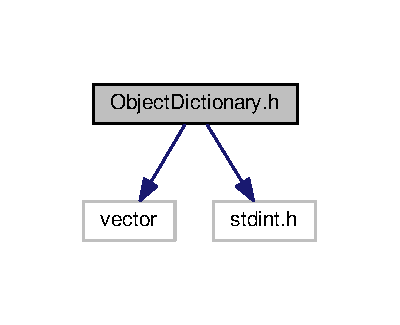
\includegraphics[width=192pt]{ObjectDictionary_8h__incl}
\end{center}
\end{figure}
This graph shows which files directly or indirectly include this file\+:\nopagebreak
\begin{figure}[H]
\begin{center}
\leavevmode
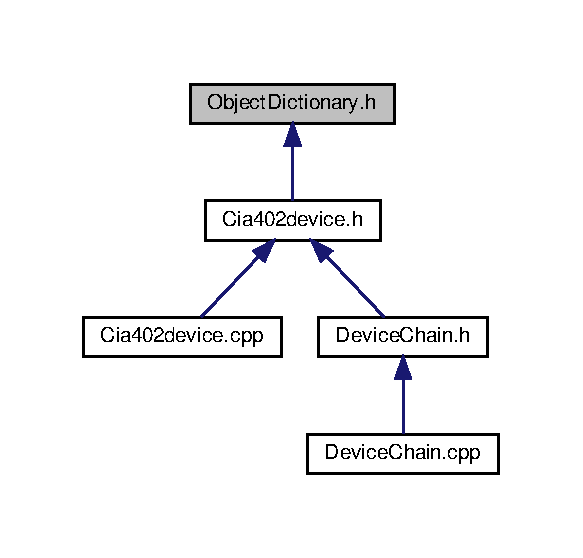
\includegraphics[width=178pt]{ObjectDictionary_8h__dep__incl}
\end{center}
\end{figure}
\subsection*{Namespaces}
\begin{DoxyCompactItemize}
\item 
 \hyperlink{namespaceod}{od}
\end{DoxyCompactItemize}
\subsection*{Variables}
\begin{DoxyCompactItemize}
\item 
const vector$<$ uint8\+\_\+t $>$ \hyperlink{namespaceod_acb23d3cf4cdb0ce0c85a884a5a97ac00}{od\+::controlword} =\{0x40,0x60\}
\item 
const vector$<$ uint8\+\_\+t $>$ \hyperlink{namespaceod_a7fe65fca00afb38d66fb49ec4fdc88c0}{od\+::statusword} =\{0x41,0x60\}
\item 
const vector$<$ uint8\+\_\+t $>$ \hyperlink{namespaceod_a75b2ed7fb6e21d4335334e1525fd223c}{od\+::commreset} =\{0x81\}
\item 
const vector$<$ uint8\+\_\+t $>$ \hyperlink{namespaceod_af9d6d0e820d6bc1ee375195e253f7b7b}{od\+::fullreset} =\{0x82\}
\item 
const vector$<$ uint8\+\_\+t $>$ \hyperlink{namespaceod_a5ca62a6451017dd2a0d53391d6fc5161}{od\+::start} =\{0x01\}
\item 
const vector$<$ uint8\+\_\+t $>$ \hyperlink{namespaceod_a360cf2eae7cc59f7bd224fcf5992c767}{od\+::goreadytoswitchon} =\{0x06,0x00\}
\item 
const vector$<$ uint8\+\_\+t $>$ \hyperlink{namespaceod_a933f995790a17f6cdd3b54df8f7483a6}{od\+::goswitchon} =\{0x07,0x00\}
\item 
const vector$<$ uint8\+\_\+t $>$ \hyperlink{namespaceod_a74448ee88df5960df4c32613e7cdcd53}{od\+::goenable} =\{0x0\+F,0x00\}
\item 
const vector$<$ uint8\+\_\+t $>$ \hyperlink{namespaceod_a12f3001ff096334fecb9c9749be4d1c2}{od\+::goswitchondisable} =\{0x00,0x00\}
\item 
const vector$<$ uint8\+\_\+t $>$ \hyperlink{namespaceod_af47128107b86d08e437f81d48d20b05a}{od\+::run} =\{0x1\+F,0x00\}
\item 
const vector$<$ uint8\+\_\+t $>$ \hyperlink{namespaceod_ae572be966c7d5de90544f2ac32dbbd38}{od\+::expedite} =\{0x3\+F,0x00\}
\item 
const vector$<$ uint8\+\_\+t $>$ \hyperlink{namespaceod_a9afdc654634df7cc336d824c594d484a}{od\+::quickstop} =\{0x02,0x00\}
\item 
const vector$<$ uint8\+\_\+t $>$ \hyperlink{namespaceod_a6f4fb30463057c20b9374a69826f6143}{od\+::\+Operation\+Mode} =\{0x60,0x60,0x00\}
\item 
const vector$<$ uint8\+\_\+t $>$ \hyperlink{namespaceod_a0469b45cd9158b638f0e0d6ed1102742}{od\+::\+Operation\+Mode\+Display} =\{0x61,0x60,0x00\}
\item 
const vector$<$ uint8\+\_\+t $>$ \hyperlink{namespaceod_a85efca0656a6714d7227858e112c4a73}{od\+::positionmode} =\{0x01\}
\item 
const vector$<$ uint8\+\_\+t $>$ \hyperlink{namespaceod_a2771fb30adf397c1cd2ddb092a414e82}{od\+::velocitymode} =\{0x03\}
\item 
const vector$<$ uint8\+\_\+t $>$ \hyperlink{namespaceod_ab5b4d34058d08a758277bf52cd31d8c9}{od\+::quick\+\_\+stop\+\_\+mode} =\{0x5\+A,0x60\}
\item 
const vector$<$ uint8\+\_\+t $>$ \hyperlink{namespaceod_af1bc07726906ffc6ea25ab9abb478143}{od\+::stop\+\_\+option\+\_\+code} =\{0x5\+D,0x60\}
\item 
const vector$<$ uint8\+\_\+t $>$ \hyperlink{namespaceod_ac4b980a10ae256ea019a767459b6ba9b}{od\+::checkerror} =\{0x02,0x10\}
\item 
const vector$<$ uint8\+\_\+t $>$ \hyperlink{namespaceod_a716df35f1a3cc3e1792c033be7fc0518}{od\+::positionaddress} =\{0x63,0x60\}
\item 
const vector$<$ uint8\+\_\+t $>$ \hyperlink{namespaceod_adf45781fb80275c184d548ea793b376b}{od\+::velocityaddress} =\{0x6\+C,0x60\}
\item 
const vector$<$ uint8\+\_\+t $>$ \hyperlink{namespaceod_a0bdcdb539c588cfae0d43cc0ba40ea05}{od\+::target\+\_\+position} =\{0x7\+A,0x60,0x00\}
\item 
const vector$<$ uint8\+\_\+t $>$ \hyperlink{namespaceod_a1d5963cb8a002987c96fae2e172790ee}{od\+::position\+\_\+demand} =\{0x62,0x60,0x00\}
\item 
const vector$<$ uint8\+\_\+t $>$ \hyperlink{namespaceod_aced8c17d62c0e774949057de0a99f402}{od\+::profile\+\_\+acceleration} =\{0x83,0x60,0x00\}
\item 
const vector$<$ uint8\+\_\+t $>$ \hyperlink{namespaceod_a57361a1a6b60fd8b93c2828fd7f5429f}{od\+::quick\+\_\+stop\+\_\+deceleration} =\{0x85,0x60,0x00\}
\item 
const vector$<$ uint8\+\_\+t $>$ \hyperlink{namespaceod_a5256e8439c66da9ab7ad06fa5f72ec1a}{od\+::motion\+\_\+profile\+\_\+type} =\{0x86,0x60\}
\item 
const vector$<$ uint8\+\_\+t $>$ \hyperlink{namespaceod_a47b7c8f6797cc134be5ee1d78d83ee50}{od\+::profile\+\_\+velocity} =\{0x81,0x60,0x00\}
\item 
const vector$<$ uint8\+\_\+t $>$ \hyperlink{namespaceod_a8d1e6a3e8180e5d64d68588ee182721c}{od\+::linear\+\_\+ramp\+\_\+trapezoidal} =\{0x00\}
\item 
const vector$<$ uint8\+\_\+t $>$ \hyperlink{namespaceod_a758ce0003cc482e5464959ed79c808e2}{od\+::target\+\_\+velocity} =\{0x\+F\+F,0x60\}
\end{DoxyCompactItemize}

\hypertarget{PortBase_8cpp}{}\section{Port\+Base.\+cpp File Reference}
\label{PortBase_8cpp}\index{Port\+Base.\+cpp@{Port\+Base.\+cpp}}
{\ttfamily \#include \char`\"{}Port\+Base.\+h\char`\"{}}\\*
Include dependency graph for Port\+Base.\+cpp\+:
\nopagebreak
\begin{figure}[H]
\begin{center}
\leavevmode
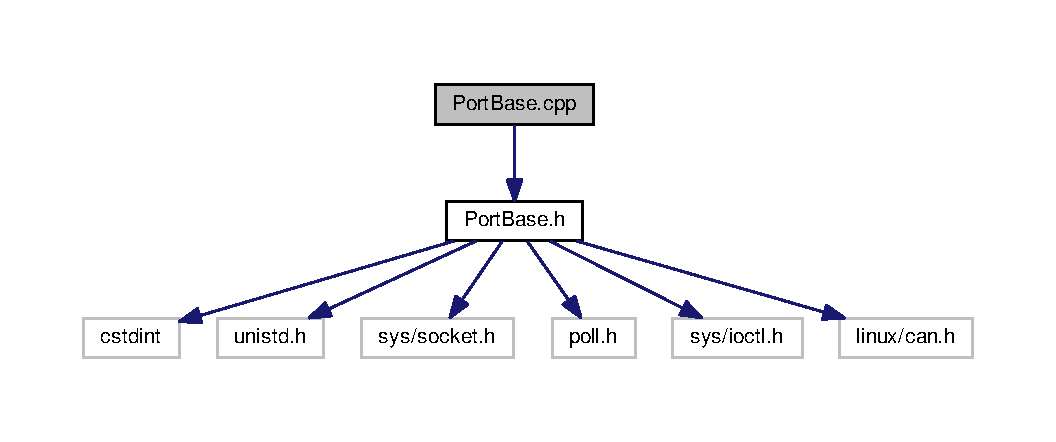
\includegraphics[width=350pt]{PortBase_8cpp__incl}
\end{center}
\end{figure}

\hypertarget{PortBase_8h}{}\section{Port\+Base.\+h File Reference}
\label{PortBase_8h}\index{Port\+Base.\+h@{Port\+Base.\+h}}
{\ttfamily \#include $<$cstdint$>$}\newline
{\ttfamily \#include $<$unistd.\+h$>$}\newline
{\ttfamily \#include $<$sys/socket.\+h$>$}\newline
{\ttfamily \#include $<$poll.\+h$>$}\newline
{\ttfamily \#include $<$sys/ioctl.\+h$>$}\newline
{\ttfamily \#include $<$linux/can.\+h$>$}\newline
Include dependency graph for Port\+Base.\+h\+:\nopagebreak
\begin{figure}[H]
\begin{center}
\leavevmode
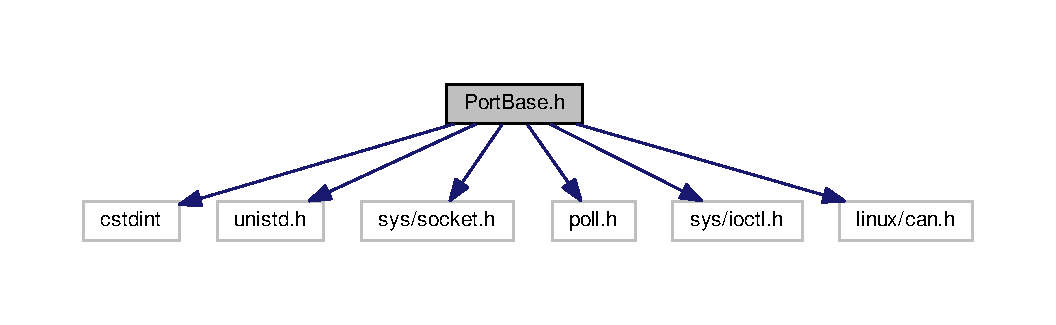
\includegraphics[width=350pt]{PortBase_8h__incl}
\end{center}
\end{figure}
This graph shows which files directly or indirectly include this file\+:\nopagebreak
\begin{figure}[H]
\begin{center}
\leavevmode
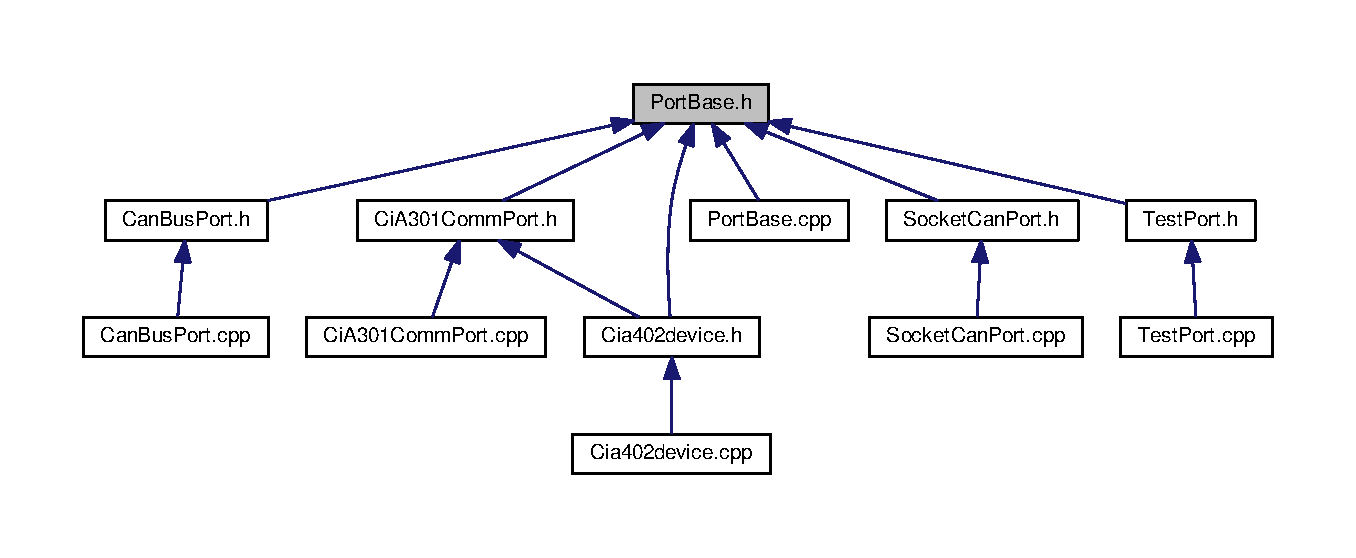
\includegraphics[width=350pt]{PortBase_8h__dep__incl}
\end{center}
\end{figure}
\subsection*{Classes}
\begin{DoxyCompactItemize}
\item 
class \hyperlink{classPortBase}{Port\+Base}
\end{DoxyCompactItemize}

\hypertarget{README_8md}{}\section{R\+E\+A\+D\+M\+E.\+md File Reference}
\label{README_8md}\index{R\+E\+A\+D\+M\+E.\+md@{R\+E\+A\+D\+M\+E.\+md}}

\hypertarget{SocketCanPort_8cpp}{}\section{Socket\+Can\+Port.\+cpp File Reference}
\label{SocketCanPort_8cpp}\index{Socket\+Can\+Port.\+cpp@{Socket\+Can\+Port.\+cpp}}
{\ttfamily \#include \char`\"{}Socket\+Can\+Port.\+h\char`\"{}}\\*
Include dependency graph for Socket\+Can\+Port.\+cpp\+:
\nopagebreak
\begin{figure}[H]
\begin{center}
\leavevmode
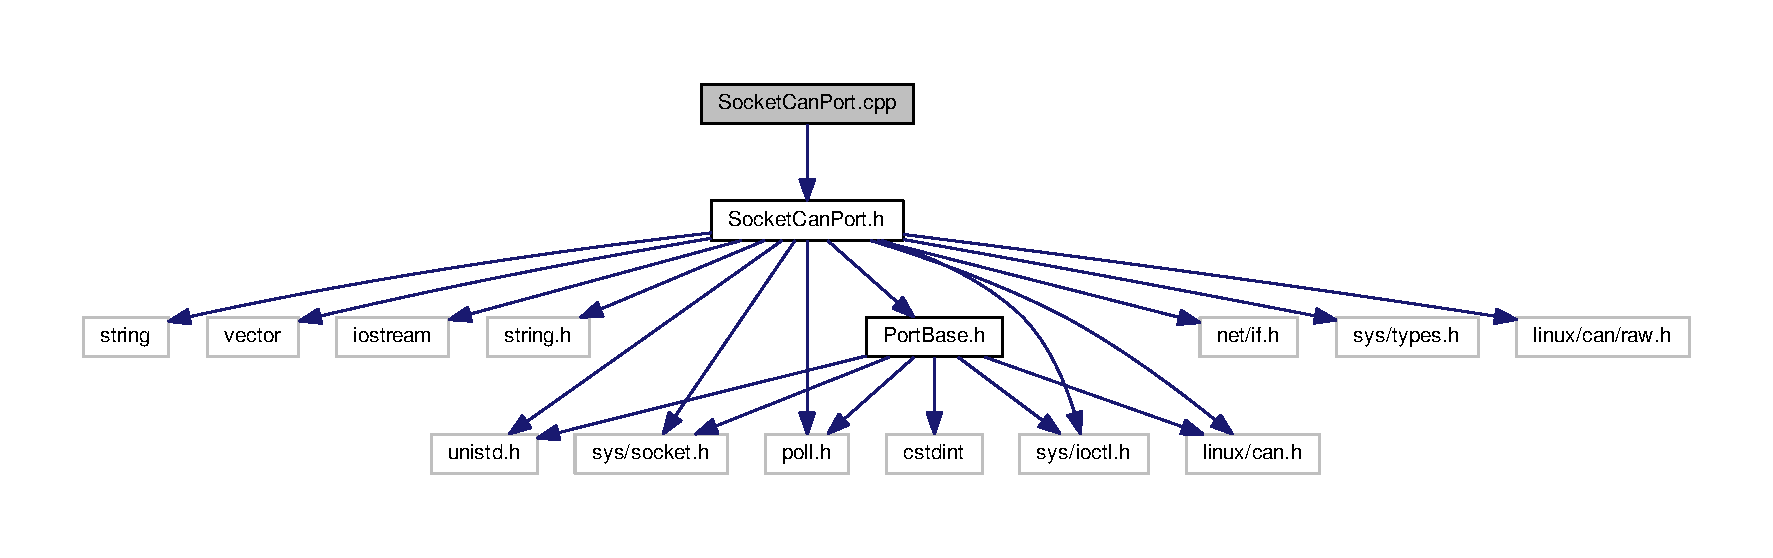
\includegraphics[width=350pt]{SocketCanPort_8cpp__incl}
\end{center}
\end{figure}

\hypertarget{SocketCanPort_8h}{}\section{Socket\+Can\+Port.\+h File Reference}
\label{SocketCanPort_8h}\index{Socket\+Can\+Port.\+h@{Socket\+Can\+Port.\+h}}
{\ttfamily \#include $<$string$>$}\newline
{\ttfamily \#include $<$vector$>$}\newline
{\ttfamily \#include $<$iostream$>$}\newline
{\ttfamily \#include $<$string.\+h$>$}\newline
{\ttfamily \#include $<$unistd.\+h$>$}\newline
{\ttfamily \#include $<$net/if.\+h$>$}\newline
{\ttfamily \#include $<$sys/types.\+h$>$}\newline
{\ttfamily \#include $<$sys/socket.\+h$>$}\newline
{\ttfamily \#include $<$poll.\+h$>$}\newline
{\ttfamily \#include $<$sys/ioctl.\+h$>$}\newline
{\ttfamily \#include $<$linux/can.\+h$>$}\newline
{\ttfamily \#include $<$linux/can/raw.\+h$>$}\newline
{\ttfamily \#include \char`\"{}Port\+Base.\+h\char`\"{}}\newline
Include dependency graph for Socket\+Can\+Port.\+h\+:\nopagebreak
\begin{figure}[H]
\begin{center}
\leavevmode
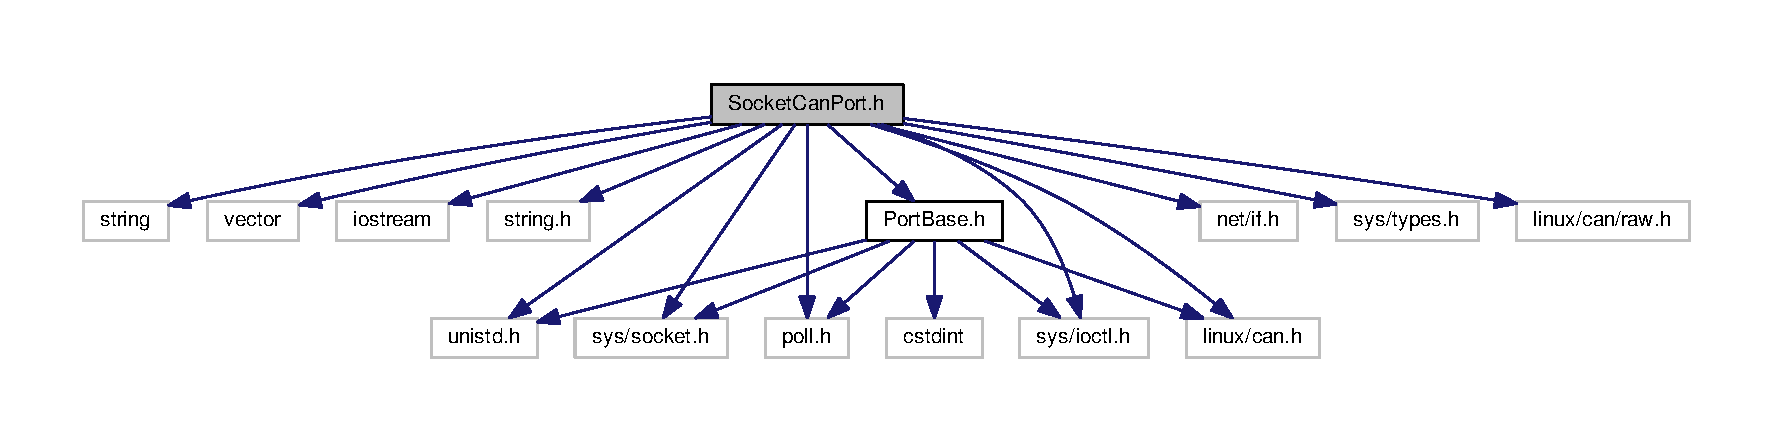
\includegraphics[width=350pt]{SocketCanPort_8h__incl}
\end{center}
\end{figure}
This graph shows which files directly or indirectly include this file\+:\nopagebreak
\begin{figure}[H]
\begin{center}
\leavevmode
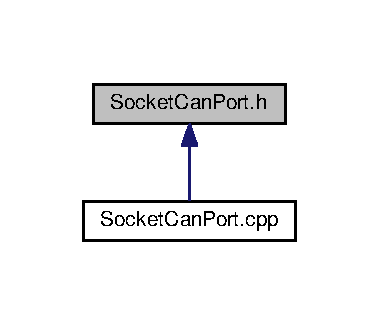
\includegraphics[width=182pt]{SocketCanPort_8h__dep__incl}
\end{center}
\end{figure}
\subsection*{Classes}
\begin{DoxyCompactItemize}
\item 
class \hyperlink{classSocketCanPort}{Socket\+Can\+Port}
\end{DoxyCompactItemize}

\hypertarget{TestPort_8cpp}{}\section{Test\+Port.\+cpp File Reference}
\label{TestPort_8cpp}\index{Test\+Port.\+cpp@{Test\+Port.\+cpp}}
{\ttfamily \#include \char`\"{}Test\+Port.\+h\char`\"{}}\newline
Include dependency graph for Test\+Port.\+cpp\+:\nopagebreak
\begin{figure}[H]
\begin{center}
\leavevmode
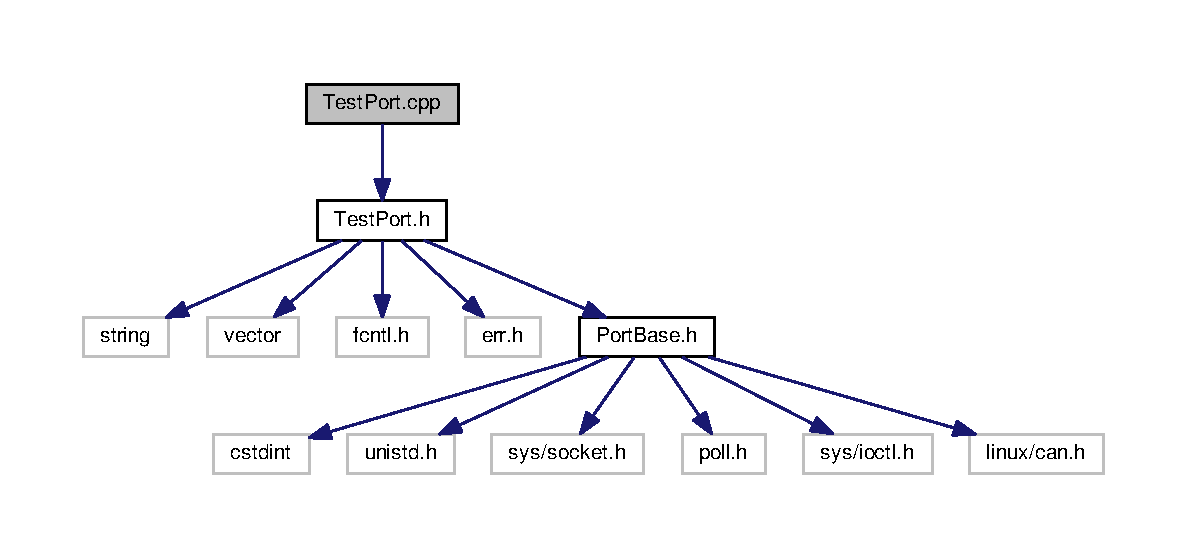
\includegraphics[width=350pt]{TestPort_8cpp__incl}
\end{center}
\end{figure}

\hypertarget{TestPort_8h}{}\section{Test\+Port.\+h File Reference}
\label{TestPort_8h}\index{Test\+Port.\+h@{Test\+Port.\+h}}
{\ttfamily \#include $<$string$>$}\newline
{\ttfamily \#include $<$vector$>$}\newline
{\ttfamily \#include $<$fcntl.\+h$>$}\newline
{\ttfamily \#include $<$err.\+h$>$}\newline
{\ttfamily \#include \char`\"{}Port\+Base.\+h\char`\"{}}\newline
Include dependency graph for Test\+Port.\+h\+:\nopagebreak
\begin{figure}[H]
\begin{center}
\leavevmode
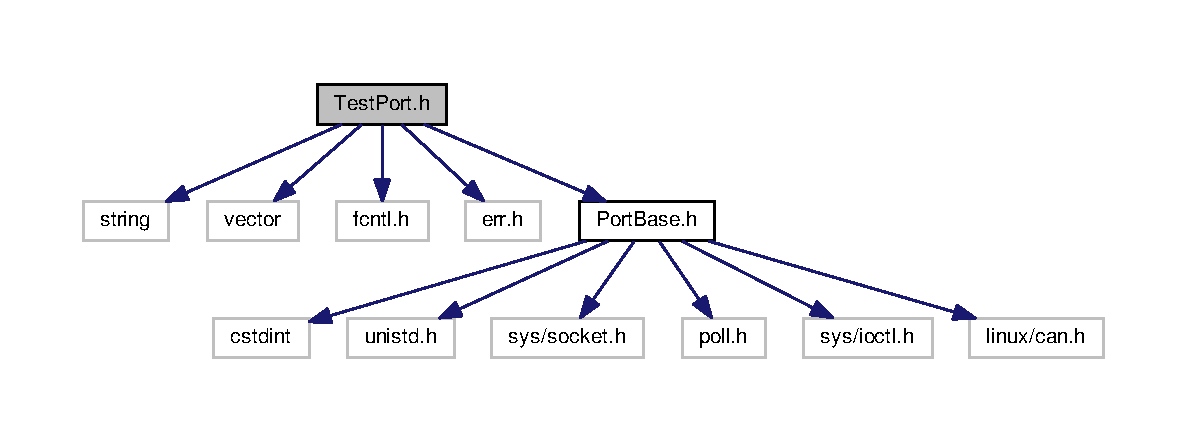
\includegraphics[width=350pt]{TestPort_8h__incl}
\end{center}
\end{figure}
This graph shows which files directly or indirectly include this file\+:\nopagebreak
\begin{figure}[H]
\begin{center}
\leavevmode
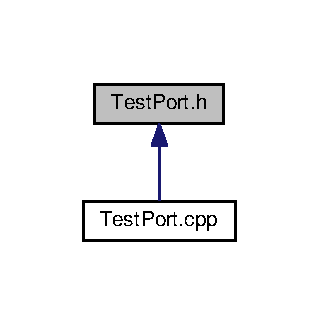
\includegraphics[width=153pt]{TestPort_8h__dep__incl}
\end{center}
\end{figure}
\subsection*{Classes}
\begin{DoxyCompactItemize}
\item 
class \hyperlink{classTestPort}{Test\+Port}
\end{DoxyCompactItemize}

%--- End generated contents ---

% Index
\backmatter
\newpage
\phantomsection
\clearemptydoublepage
\addcontentsline{toc}{chapter}{Index}
\printindex

\end{document}
